\documentclass[letterpaper,10pt]{book}
% Change to 10 pt
\usepackage{pdfpages}
\usepackage{morewrites}			% to counteract the no write space problem
\setcounter{tocdepth}{6}

\usepackage[framemethod=TikZ]{mdframed}

\usepackage{fancyhdr}

\usepackage{paralist}
\usepackage{amsmath}
\usepackage{amsfonts}
\usepackage{amssymb}
\usepackage{graphicx}

\usepackage{datetime}
%\usepackage{ulem}

%\usepackage[nottoc]{toobibind}

\usepackage[inline]{enumitem}

% Outer margin at 2.50 is exacty correct to fit the ``corruption alert'' tables
\usepackage[inner=1.0in, outer=2.50in, top=2.54cm,bottom=2.54cm, marginparwidth=2.25in]{geometry}

\usepackage{marginnote}
\usepackage{longtable}
\usepackage{booktabs}
\usepackage{xcolor}

\usepackage{soul}

%%%%%%%%%%%%
\definecolor{ForestGreen}{rgb}{0.00,0.29,0.098}
%%%%%%%%%%%%

\usepackage{marginnote}

\usepackage{imakeidx} 
\usepackage[
	backref=true,
	style=numeric,
%	citestyle=numeric,
	backend=bibtex
	]{biblatex}
\usepackage[driverfallback=hypertex,colorlinks=True]{hyperref}
\usepackage{cleveref}

\makeindex[name=scripture,columnsep=20pt, columnseprule=True,columns=3, title=Scripture References]
\makeindex[name=speaker,columnsep=20pt, columnseprule=True,,columns=2, title=Sermon Creator]
\makeindex[name=series,columnsep=20pt, columnseprule=True,,columns=2, title=Sermon Series]
\makeindex[name=date,columnsep=20pt, columnseprule=True,columns=2, title=Sermon Date]
\makeindex[name=event,columnsep=20pt, columnseprule=True,columns=2, title=Event]
\makeindex[name=topic,columnsep=20pt, columnseprule=True,columns=2, title=Topic]
\makeindex[name=AWIP,columnsep=20pt, columnseprule=True,columns=3, title=All Words in Passage]
\makeindex[name=NWIV,columnsep=20pt, columnseprule=True,columns=3, title=Number of Words in Verse]
\makeindex[name=PNIP,columnsep=20pt, columnseprule=True,columns=3, title=Proper Names in Passage]
\makeindex[name=PEIP,columnsep=20pt, columnseprule=True,columns=2, title=Prophetic Events in Passage]
\makeindex[name=TWPAQ,columnsep=20pt, columnseprule=True,columns=1, title=13-Word Phrases and Quotes]
\makeindex[name=PFTTIS,columnsep=20pt, columnseprule=False,columns=3, title=Phrases found 13 times in scripture]
\makeindex[name=WFTTIS,columnsep=20pt, columnseprule=False,columns=3, title=Words found 13 times in scripture]
\makeindex[name=WFITV,columnsep=20pt, columnseprule=False,columns=3, title=Words found in exactly 13 verses]
\makeindex[name=EVENTS,columnsep=20pt, columnseprule=False,columns=2, title=Sermon Log by Place]
\makeindex[name=QUESTIONS,columnsep=20pt, columnseprule=False,columns=2, title=Bible Questions]
\makeindex[name=DOCTRINES,columnsep=20pt, columnseprule=False,columns=2, title=Doctrines]
\makeindex[name=SONGS,columnsep=20pt, columnseprule=False,columns=1, title=Songs]
\makeindex[name=LOCATION,columnsep=20pt, columnseprule=False,columns= 2, title=Location]
\makeindex[name=FACEBOOK,columnsep=20pt, columnseprule=False,columns=2, title=Facebook]
\makeindex[name=DEVOTIONAL,columnsep=20pt, columnseprule=False,columns=2, title=Devotional Items]
%%%%%%%%%%%%%%%%% EXTRA COLORS
\definecolor{champagne}{rgb}{0.97,0.91,0.81}
\definecolor{bone}{rgb}{0.89,0.85,0.79}
\pagestyle{fancy}
\fancyhf{}
\fancyhead[LE,RO]{\today}
\fancyhead[RE,LO]{Daily Bible Reading}
\fancyhead[CE,CO]{-page \thepage  - }

\fancyfoot[CO,CE]{\leftmark}
%\fancyfoot[LE,RO]{CSCE 692, HW1}

\title{DBR\\
Daily \\ Reads}
\author{Keith Anthony \\
\today }
%+/ffffff +   \pagenumbering{gobble}
\bibliography{Bibliographies/All20220122}

\setlength{\fboxsep}{1.0pt}

\usepackage[utf8]{inputenc}
\usepackage{tikz}

\begin{document}
%%%%%%%%%%%% Tile Page

\begin{titlepage}

\begin{flushright}
\rightskip=-2.5cm
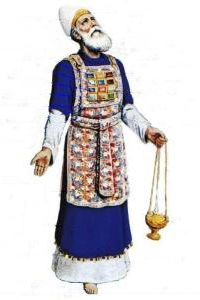
\includegraphics[width=50mm,scale=1.5]{Extras/Melchisedec.jpg}
\vspace{0.4in}  % Create a title for the document and write it in bold font
\LARGE{\textbf{\date}} % Again, do a line break
\linebreak 
% Create a subtitle \large{with Outlines, Statistics, Cross References, and Notes}
\vspace{0.5in}
\begin{flushleft}
\LARGE{Day \#66: Monday, 7 March 2022  \\}\vspace{0.25in}
\LARGE{Joshua 4-6 Psalm 66 Proverb 7}
\end{flushleft}
\vspace{0.6in}
\bigskip

\normalsize{Xenia, Oh.\\}
\normalsize{created: \today}
\vspace{1.3in}

\end{flushright}
\end{titlepage}

\newpage 
\tableofcontents\hypertarget{TOC}{}
\listoffigures
\listoftables

\hyphenation{A-bim-e-lech bre-thren E-phra-im  Gib-e-o-nites Jer-u-sa-lem through-out Phil-i-stines The-o-phil-us Am-a-le-kites ven-geance Mesh-el-e-mi-ah onan-ism Phar-a-oh thoughts grev-ous-ness Hach-a-liah adul-ter-er Shad-rach}

%%%%%%%%%%%%%%%%% EXTRA COLORS
%%%%%%%%%%%%%%%%% EXTRA COLORS
%%%%%%%%%%%%%%%%% EXTRA COLORS
\definecolor{champagne}{rgb}{0.97,0.91,0.81}
\definecolor{bone}{rgb}{0.89,0.85,0.79}

\definecolor{ForestGreen}{rgb}{0.00,0.29,0.098}
\definecolor{GIVING}{cmyk}{1,0.0,0.72,.1}

\definecolor{MLPE}{cmyk}{1,1,0,.45}
\definecolor{SOCCER}{cmyk}{.77, 0, .42, .49}
\definecolor{PAYBILL}{cmyk}{0,0.83,0.76,0.07}
\definecolor{SERMON}{cmyk}{.14,.9,0,.30} % aka seance \href{http://www.flatuicolorpicker.com/purple-cmyk-color-model/}{seance}
\definecolor{BIBLE}{cmyk}{0,.17,.74,.17}
\definecolor{WORKBLUE}{cmyk}{1, .5, 0, .6}
\definecolor{myOrange}{cmyk}{0, .4, .98, .03}
\definecolor{myTan}{cmyk}{0.0,.07,.17,.10}
\definecolor{myRed}{cmyk}{0,1,1,0}
\definecolor{myWhite}{cmyk}{0,0,0,0}
\definecolor{BLUESoD}{cmyk}{.97,.84,0,.04}
\definecolor{WHITE}{cmyk}{0,0,0,0}
\definecolor{OLDGOLD}{cmyk}{0.05,0.3,1.00,0}
\definecolor{CASTLETON}{cmyk}{1,0,0.31,0.66}
\definecolor{cadmiumgreen}{rgb}{0.0, 0.42, 0.24}
\definecolor{jungle}{rgb}{0.203,0.4882,0.1718}
\definecolor{MYGOLD}{rgb}{1,.84,0}

\definecolor{MYLIGHTGRAY}{rgb}{.85,.85,.85}

\definecolor{codegreen}{rgb}{0,0.6,0}
\definecolor{codegray}{rgb}{0.5,0.5,0.5}
\definecolor{codepurple}{rgb}{0.58,0,0.82}
\definecolor{backcolour}{rgb}{0.95,0.95,0.92}


\mdfdefinestyle{MyFrame}{%
    linecolor=blue,
    outerlinewidth=2pt,
    roundcorner=5pt,
    innertopmargin=\baselineskip,
    innerbottommargin=\baselineskip,
    innerrightmargin=10pt,
    innerleftmargin=10pt,
    backgroundcolor=gray!25!white}


\mdfdefinestyle{MyFrame2}{%
    linecolor=black,
    outerlinewidth=2pt,
    roundcorner=5pt,
    innertopmargin=\baselineskip,
    innerbottommargin=\baselineskip,
    innerrightmargin=10pt,
    innerleftmargin=10pt,
    backgroundcolor=yellow!25!white}


%%%%%
%% for PFTTIS list
%%%%%

%%% And Joseph said unto
\index[PFTTIS]{And Joseph said unto!Genesis!Gen 40:008}
\index[PFTTIS]{And Joseph said unto!Genesis!Gen 40:012}
\index[PFTTIS]{And Joseph said unto!Genesis!Gen 41:025}
\index[PFTTIS]{And Joseph said unto!Genesis!Gen 42:014}
\index[PFTTIS]{And Joseph said unto!Genesis!Gen 42:018}
\index[PFTTIS]{And Joseph said unto!Genesis!Gen 44:015}
\index[PFTTIS]{And Joseph said unto!Genesis!Gen 45:003}
\index[PFTTIS]{And Joseph said unto!Genesis!Gen 45:004}
\index[PFTTIS]{And Joseph said unto!Genesis!Gen 46:031}
\index[PFTTIS]{And Joseph said unto!Genesis!Gen 48:009}
\index[PFTTIS]{And Joseph said unto!Genesis!Gen 48:018}
\index[PFTTIS]{And Joseph said unto!Genesis!Gen 50:019}
\index[PFTTIS]{And Joseph said unto!Genesis!Gen 50:024}


%%% a shadow
\index[PFTTIS]{a shadow!1Chronicles!1Chr 029:15}
\index[PFTTIS]{a shadow!Job!Job 008:09}
\index[PFTTIS]{a shadow!Job!Job 014:02}
\index[PFTTIS]{a shadow!Job!Job 017:07}
\index[PFTTIS]{a shadow!Psalm!Psa 102:011}
\index[PFTTIS]{a shadow!Psalm!Psa 144:004}
\index[PFTTIS]{a shadow!Ecclesiastes!Eccl 006:012}
\index[PFTTIS]{a shadow!Ecclesiastes!Eccl 008:013}
\index[PFTTIS]{a shadow!Isaiah!Isa 04:006}
\index[PFTTIS]{a shadow!Isaiah!Isa 25:004}
\index[PFTTIS]{a shadow!Jonah!Jnh 04:06}
\index[PFTTIS]{a shadow!Colossians!Col 02:017}
\index[PFTTIS]{a shadow!Hebews!Heb 10:001}

%%% blessed is the man
\index[PFTTIS]{blessed is the man!Psalm!Psa 001:001}
\index[PFTTIS]{blessed is the man!Psalm!Psa 032:002}
\index[PFTTIS]{blessed is the man!Psalm!Psa 034:008}
\index[PFTTIS]{blessed is the man!Psalm!Psa 065:004}
\index[PFTTIS]{blessed is the man!Psalm!Psa 084:005}
\index[PFTTIS]{blessed is the man!Psalm!Psa 084:012}
\index[PFTTIS]{blessed is the man!Psalm!Psa 094:012}
\index[PFTTIS]{blessed is the man!Psalm!Psa 112:001}
\index[PFTTIS]{blessed is the man!Proverbs!Pro 008:034}
\index[PFTTIS]{blessed is the man!Isaiah!Isa 056:002}
\index[PFTTIS]{blessed is the man!Jeremiah!Jer 017:007}
\index[PFTTIS]{blessed is the man!Romans!Rom 004:008}
\index[PFTTIS]{blessed is the man!James!Jam 001:012}


%%% carry them
\index[PFTTIS]{carry them!Leviticus!Lev 14:045}
\index[PFTTIS]{carry them!Numbers!Num 11:012}
\index[PFTTIS]{carry them!Joshua!Jsh 04:003}
\index[PFTTIS]{carry them!1Samuel!1Sam 20:040}
\index[PFTTIS]{carry them!1Kings!1Kng 08:046}
\index[PFTTIS]{carry them!2Chronicles!2Chr 06:036}
\index[PFTTIS]{carry them!Ezra!Ezra 05:015}
\index[PFTTIS]{carry them!Isaiah!Isa 40:011}
\index[PFTTIS]{carry them!Isaiah!Isa 41:016}
\index[PFTTIS]{carry them!Isaiah!Isa 57:013}
\index[PFTTIS]{carry them!Jeremiah!Jer 20:004}
\index[PFTTIS]{carry them!Jeremiah!Jer 20:005}
\index[PFTTIS]{carry them!Jeremiah!Jer 43:012}


\index[PFTTIS]{good tidings!2Samuel!2Sam 18:027}
\index[PFTTIS]{good tidings!1Kings!1Ki 01:042}
\index[PFTTIS]{good tidings!2Kings!2Ki 07:009 (2x)}
\index[PFTTIS]{good tidings!Isaiah!Isa 40:009 (2x)}
\index[PFTTIS]{good tidings!Isaiah!Isa 41:007}
\index[PFTTIS]{good tidings!Isaiah!Isa 52:007}
\index[PFTTIS]{good tidings!Isaiah!Isa 61:001}
\index[PFTTIS]{good tidings!Nahum!Nah 01:005}
\index[PFTTIS]{good tidings!Luke!Lk 02:010}
\index[PFTTIS]{good tidings!1Thessalonians!1Thess 03:006}


%%% dead body
\index[PFTTIS]{dead body!Leviticus!Lev 21:011}
\index[PFTTIS]{dead body!Numbers!Num 06:006}
\index[PFTTIS]{dead body!Numbers!Num 09:006}
\index[PFTTIS]{dead body!Numbers!Num 09:007}
\index[PFTTIS]{dead body!Numbers!Num 09:010}
\index[PFTTIS]{dead body!Numbers!Num 09:011}
\index[PFTTIS]{dead body!Numbers!Num 09:013}
\index[PFTTIS]{dead body!Numbers!Num 09:016}
\index[PFTTIS]{dead body!2Kings!2Ki 08:005}
\index[PFTTIS]{dead body!Isaiah!Isa 26:019}
\index[PFTTIS]{dead body!Jeremiah!Jer 26:023}
\index[PFTTIS]{dead body!Jeremiah!Jer 36:030}
\index[PFTTIS]{dead body!Haggai!Hag 02:013}

%%% great sea
\index[PFTTIS]{great sea!Numbers!Num 34:006}
\index[PFTTIS]{great sea!Numbers!Num 34:007}
\index[PFTTIS]{great sea!Joshua!Jos 01:004}
\index[PFTTIS]{great sea!Joshua!Jos 09:001}
\index[PFTTIS]{great sea!Joshua!Jos 15:012}
\index[PFTTIS]{great sea!Joshua!Jos 15:047}
\index[PFTTIS]{great sea!Joshua!Jos 23:004}
\index[PFTTIS]{great sea!Ezekiel!Eze 47:010}
\index[PFTTIS]{great sea!Ezekiel!Eze 47:015}
\index[PFTTIS]{great sea!Ezekiel!Eze 47:019}
\index[PFTTIS]{great sea!Ezekiel!Eze 47:020}
\index[PFTTIS]{great sea!Ezekiel!Eze 48:028}
\index[PFTTIS]{great sea!Daniel!Dan 07:002}


%%% have forsaken me
\index[PFTTIS]{have forsaken me!Judges!Jdg 10:013}
\index[PFTTIS]{have forsaken me!1Samuel!1Sam 08:008}
\index[PFTTIS]{have forsaken me!1Kings!1Ki 11:033}
\index[PFTTIS]{have forsaken me!2Kings!2Ki 22:017}
\index[PFTTIS]{have forsaken me!2Chronicles!2Chr 12:005}
\index[PFTTIS]{have forsaken me!2Chronicles!2Chr 34:025}
\index[PFTTIS]{have forsaken me!Jeremiah!Jer 01:016}
\index[PFTTIS]{have forsaken me!Jeremiah!Jer 02:013}
\index[PFTTIS]{have forsaken me!Jeremiah!Jer 05:007}
\index[PFTTIS]{have forsaken me!Jeremiah!Jer 05:019}
\index[PFTTIS]{have forsaken me!Jeremiah!Jer 16:011 (2x)}
\index[PFTTIS]{have forsaken me!Jeremiah!Jer 19:004}

%%% no king
\index[PFTTIS]{no king!Judges!Jdg 17:06}
\index[PFTTIS]{no king!Judges!Jdg 18:01}
\index[PFTTIS]{no king!Judges!Jdg 19:01}
\index[PFTTIS]{no king!Judges!Jdg 21:25}
\index[PFTTIS]{no king!1Kings!1Ki 22:47}
\index[PFTTIS]{no king!2Kings!2Ki 23:25}
\index[PFTTIS]{no king!Nehemiah!Neh 13:26}
\index[PFTTIS]{no king!Psalms!Psa 033:016}
\index[PFTTIS]{no king!Proverbs!Pro 30:27}
\index[PFTTIS]{no king!Daniel!Dan 02:10}
\index[PFTTIS]{no king!Hosea!Hos 10:03}
\index[PFTTIS]{no king!Micah!Mic 04:09}
\index[PFTTIS]{no king!John!Jhn 19:15}


%%% rebellious house
\index[PFTTIS]{rebellious house!Exodus!Exo 02:005}
\index[PFTTIS]{rebellious house!Exodus!Exo 02:006}
\index[PFTTIS]{rebellious house!Exodus!Exo 02:008}
\index[PFTTIS]{rebellious house!Exodus!Exo 03:009}
\index[PFTTIS]{rebellious house!Exodus!Exo 03:026}
\index[PFTTIS]{rebellious house!Exodus!Exo 03:027}
\index[PFTTIS]{rebellious house!Exodus!Exo 12:002 (2x)}
\index[PFTTIS]{rebellious house!Exodus!Exo 12:003}
\index[PFTTIS]{rebellious house!Exodus!Exo 12:009}
\index[PFTTIS]{rebellious house!Exodus!Exo 12:025}
\index[PFTTIS]{rebellious house!Exodus!Exo 17:012}
\index[PFTTIS]{rebellious house!Exodus!Exo 24:003}

%%% seek him
\index[PFTTIS]{seek him!Deuteronomy!Deu 04:029}\index[PFTTIS]{seek him!1Samuel!1Sam 23:025}
\index[PFTTIS]{seek him!1Chronicles!1Chr 28:009}
\index[PFTTIS]{seek him!2Chronicles!1Chr 15:002}
\index[PFTTIS]{seek him!Ezra!Ezr 08:022}
\index[PFTTIS]{seek him!Psalms!Psa 022:026}
\index[PFTTIS]{seek him!Psalms!Psa 024:006}
\index[PFTTIS]{seek him!Psalms!Psa 119:002}
\index[PFTTIS]{seek him!SoS!SoS 03:002}
\index[PFTTIS]{seek him!SoS!SoS 06:001}
\index[PFTTIS]{seek him!Hosea!Hos 07:010}
\index[PFTTIS]{seek him!Amos!Amo 05:008}
\index[PFTTIS]{seek him!Hebrews!Heb 11:0063}


%%% seek ye
\index[PFTTIS]{seek ye!Isaiah!Isa 34:016}
\index[PFTTIS]{seek ye!Isaiah!Isa 45:019}
\index[PFTTIS]{seek ye!Isaiah!Isa 55:006}
\index[PFTTIS]{seek ye!Amos!Amos 5:004}
\index[PFTTIS]{seek ye!John!John 1:38}
\index[PFTTIS]{seek ye!John!John 18:4}
\index[PFTTIS]{seek ye!John!John 18:7}
\index[PFTTIS]{seek ye!Matthew!Matt 6:33}
\index[PFTTIS]{seek ye!Numbers!Num 16:10}
\index[PFTTIS]{seek ye!Luke!Luke 12:31}
\index[PFTTIS]{seek ye!Luke!Luke 24:5}
\index[PFTTIS]{seek ye!Psalm!Psa 27:8}
\index[PFTTIS]{seek ye!Zephaniah!Zeph 2:3}

%%% the uncircumcised
\index[PFTTIS]{the uncircumcised!Genesis!Gen 17:014}
\index[PFTTIS]{the uncircumcised!Judges!Jdg 14:003}
\index[PFTTIS]{the uncircumcised!Judges!Jdg 15:018}
\index[PFTTIS]{the uncircumcised!2Samuel!2Sam 01:020}
\index[PFTTIS]{the uncircumcised!Isaiah!Isa 02:001}
\index[PFTTIS]{the uncircumcised!Jeremiah!Jer 09:025}
\index[PFTTIS]{the uncircumcised!Ezekiel!Eze 28:010}
\index[PFTTIS]{the uncircumcised!Ezekiel!Eze 31:018}
\index[PFTTIS]{the uncircumcised!Ezekiel!Eze 32:019}
\index[PFTTIS]{the uncircumcised!Ezekiel!Eze 32:027}
\index[PFTTIS]{the uncircumcised!Ezekiel!Eze 32:028}
\index[PFTTIS]{the uncircumcised!Ezekiel!Eze 32:029}
\index[PFTTIS]{the uncircumcised!Ezekiel!Eze 32:032}

%%% worship him
\index[PFTTIS]{worship him!Psalms!Psa 97:007}
\index[PFTTIS]{worship him!Zephaniah!Zeph 02:011}
\index[PFTTIS]{worship him!Matthew!Matt 02:002}
\index[PFTTIS]{worship him!Matthew!Matt 02:008}
\index[PFTTIS]{worship him!John!John 04:023}
\index[PFTTIS]{worship him!John!John 04:024 (2x)} 
\index[PFTTIS]{worship him!Acts!Acts 17:023}
\index[PFTTIS]{worship him!Hebrews!Heb 01:006}
\index[PFTTIS]{worship him!Revelation!Rev 04:010}
\index[PFTTIS]{worship him!Revelation!Rev 13:008}
\index[PFTTIS]{worship him!Revelation!Rev 14:007}
\index[PFTTIS]{worship him!Revelation!Rev 19:010}


%%%%%
%% for PFTTIS list
%%%%%

%%% afflictions
\index[WFTTIS]{afflictions!Psalms!Psa 34:019}
\index[WFTTIS]{afflictions!Psalms!Psa 132:001}
\index[WFTTIS]{afflictions!Acts!Acts 07:010}
\index[WFTTIS]{afflictions!Acts!Acts 20:023}
\index[WFTTIS]{afflictions!2Corinthians!2Cor 06:004}
\index[WFTTIS]{afflictions!Colossians!Col 01:024}
\index[WFTTIS]{afflictions!1Thessalonians!1Thess 03:003}
\index[WFTTIS]{afflictions!2Timothy!2Tim 01:008}
\index[WFTTIS]{afflictions!2Timothy!2Tim 03:011}
\index[WFTTIS]{afflictions!2Timothy!2Tim 04:005}
\index[WFTTIS]{afflictions!Hebrews!Heb 10:032}
\index[WFTTIS]{afflictions!Hebrews!Heb 10:033}
\index[WFTTIS]{afflictions!1Peter!1Pet 05:009}

%%% acsend
\index[WFTTIS]{acsend!Joshua!Jos 06:05}
\index[WFTTIS]{acsend!Psalm!Psa 024:003}
\index[WFTTIS]{acsend!Psalm!Psa 135:007}
\index[WFTTIS]{acsend!Psalm!Psa 139:008}
\index[WFTTIS]{acsend!Isaiah!Isa 14:013}
\index[WFTTIS]{acsend!Isaiah!Isa 14:014}
\index[WFTTIS]{acsend!Jeremiah!Jer 10:013}
\index[WFTTIS]{acsend!Jeremiah!Jer 51:016}
\index[WFTTIS]{acsend!Ezekiel!Eze 38:009}
\index[WFTTIS]{acsend!John!John 06:062}
\index[WFTTIS]{acsend!John!John 20:017}
\index[WFTTIS]{acsend!Romans!Rom 10:006}
\index[WFTTIS]{acsend!Revelation!Rev 17:008}

%%% Assyrian
\index[WFTTIS]{Assyrian!Isaiah!Isa 10:005}
\index[WFTTIS]{Assyrian!Isaiah!Isa 10:024}
\index[WFTTIS]{Assyrian!Isaiah!Isa 14:025}
\index[WFTTIS]{Assyrian!Isaiah!Isa 19:023}
\index[WFTTIS]{Assyrian!Isaiah!Isa 23:013}
\index[WFTTIS]{Assyrian!Isaiah!Isa 30:031}
\index[WFTTIS]{Assyrian!Isaiah!Isa 31:008}
\index[WFTTIS]{Assyrian!Isaiah!Isa 52:004}
\index[WFTTIS]{Assyrian!Ezekiel!Eze 31:003}
\index[WFTTIS]{Assyrian!Hosea!Hos 05:013}
\index[WFTTIS]{Assyrian!Hosea!Hos 11:005}
\index[WFTTIS]{Assyrian!Micah!Hos 05:005}
\index[WFTTIS]{Assyrian!Micah!Hos 05:006}

%%% blot
\index[WFTTIS]{blot!Exodus!Exo 32:032}
\index[WFTTIS]{blot!Exodus!Exo 32:033}
\index[WFTTIS]{blot!Numbers!Num 05:026}
\index[WFTTIS]{blot!Deuteronomy!Deut 09:014}
\index[WFTTIS]{blot!Deuteronomy!Deut 25:019}
\index[WFTTIS]{blot!Deuteronomy!Deut 29:020}
\index[WFTTIS]{blot!2Kings!2Ki 14:027}
\index[WFTTIS]{blot!Job!Job 31:007}
\index[WFTTIS]{blot!Psalms!Psa 51:001}
\index[WFTTIS]{blot!Psalms!Psa 51:009}
\index[WFTTIS]{blot!Proverbs!Pro 09:007}
\index[WFTTIS]{blot!Jeremiah!Jer 18:023}
\index[WFTTIS]{blot!Revelation!Rev 03:005}


%%% chain
\index[WFTTIS]{chain!Genesis!Gen 41:042}
\index[WFTTIS]{chain!1Kings!1Ki 07:017}
\index[WFTTIS]{chain!Psalms!Psa 73:006}
\index[WFTTIS]{chain!SoS!Sos 04:009}
\index[WFTTIS]{chain!Lamentations!Lam 03:007}
\index[WFTTIS]{chain!Ezekiel!Eze 07:023}
\index[WFTTIS]{chain!Ezekiel!Eze 16:011}
\index[WFTTIS]{chain!Daniel!Dan 05:007}
\index[WFTTIS]{chain!Daniel!Dan 05:016}
\index[WFTTIS]{chain!Daniel!Dan 05:029}
\index[WFTTIS]{chain!Acts!Acts 28:020}
\index[WFTTIS]{chain!2Timothy!2Tim 01:016}
\index[WFTTIS]{chain!Revelation!Rev 20:001}


%%% controversy
\index[WFTTIS]{controversy!Deuteronomy!Deu 17:008}
\index[WFTTIS]{controversy!Deuteronomy!Deu 19:017}
\index[WFTTIS]{controversy!Deuteronomy!Deu 21:005}
\index[WFTTIS]{controversy!Deuteronomy!Deu 25:001}
\index[WFTTIS]{controversy!2Samuel!2Sam 15:002}
\index[WFTTIS]{controversy!Isaiah!Isa 34:008}
\index[WFTTIS]{controversy!Jeremiah!Jer 25:031}
\index[WFTTIS]{controversy!Ezekiel!Eze 44:024}
\index[WFTTIS]{controversy!Hosea!Hos 04:001}
\index[WFTTIS]{controversy!Hosea!Hos 12:002}
\index[WFTTIS]{controversy!Micah!Mic 06:002 (2x)}
\index[WFTTIS]{controversy!1Timothy!1Tim 03:016}


%%% Dagon/Dagon's
\index[WFTTIS]{Dagon!Judges!Jdg 16:023}
\index[WFTTIS]{Dagon!1Samuel!1Sam 05:002 (2x)}
\index[WFTTIS]{Dagon!1Samuel!1Sam 05:003 (2x)}
\index[WFTTIS]{Dagon!1Samuel!1Sam 05:004 (3x)}
\index[WFTTIS]{Dagon!1Samuel!1Sam 05:005 (3x)}
\index[WFTTIS]{Dagon!1Samuel!1Sam 05:007}
\index[WFTTIS]{Dagon!1Chronicles!1Chr 10:010}

%%% disobedient
\index[WFTTIS]{disobedient!1Kings!1Ki 13:026}
\index[WFTTIS]{disobedient!Nehemiah!Neh 09:026}
\index[WFTTIS]{disobedient!Luke!Luke 01:017}
\index[WFTTIS]{disobedient!Acts!Acts 26:019}
\index[WFTTIS]{disobedient!Romans!Rom 01:030}
\index[WFTTIS]{disobedient!Romans!Rom 10:021}
\index[WFTTIS]{disobedient!1Timothy!1Tim 01:009}
\index[WFTTIS]{disobedient!2Timothy!2Tim 03:002}
\index[WFTTIS]{disobedient!Titus!Titus 01:016}
\index[WFTTIS]{disobedient!Titus!Titus 03:003}
\index[WFTTIS]{disobedient!1Peter!1Pet 02:007}
\index[WFTTIS]{disobedient!1Peter!1Pet 02:008}
\index[WFTTIS]{disobedient!1Peter!1Pet 03:020}


%%% doubt
\index[WFTTIS]{doubt!Genesis!Gen 37:033}
\index[WFTTIS]{doubt!Deuteronomy!Deu 28:066}
\index[WFTTIS]{doubt!Job!Job 12:002}
\index[WFTTIS]{doubt!Matthew!Matt 14:031}
\index[WFTTIS]{doubt!Matthew!Matt 21:021}
\index[WFTTIS]{doubt!Mark!Mk 11:023}
\index[WFTTIS]{doubt!Luke!Lk 11:020}
\index[WFTTIS]{doubt!John!Jhn 10:024}
\index[WFTTIS]{doubt!Acts!Acts 02:012}
\index[WFTTIS]{doubt!Acts!Acts 28:004}
\index[WFTTIS]{doubt!1Corinthians!1Cor 09:010}
\index[WFTTIS]{doubt!Galatians!Gal 04:020}
\index[WFTTIS]{doubt!1John!1Jhn 02:019}


%%% dungeon
\index[WFTTIS]{dungeon!Genesis!Gen 40:015}
\index[WFTTIS]{dungeon!Genesis!Gen 41:014}
\index[WFTTIS]{dungeon!Exodus!Exo 12:029}
\index[WFTTIS]{dungeon!Jeremiah!Jer 37:016}
\index[WFTTIS]{dungeon!Jeremiah!Jer 38:006 (2x)}
\index[WFTTIS]{dungeon!Jeremiah!Jer 38:007}
\index[WFTTIS]{dungeon!Jeremiah!Jer 38:009}
\index[WFTTIS]{dungeon!Jeremiah!Jer 38:010}
\index[WFTTIS]{dungeon!Jeremiah!Jer 38:011}
\index[WFTTIS]{dungeon!Jeremiah!Jer 38:013}
\index[WFTTIS]{dungeon!Lamentations!Lam 03:053}
\index[WFTTIS]{dungeon!Lamentations!Lam 03:055}


%%% error
\index[WFTTIS]{error!2Samuel!2Sam 06:007}
\index[WFTTIS]{error!Job!Job 19:004}
\index[WFTTIS]{error!Ecclesiastes!Ecc 05:006}
\index[WFTTIS]{error!Ecclesiastes!Ecc 10:005}
\index[WFTTIS]{error!Isaiah!Isa 32:006}
\index[WFTTIS]{error!Daniel!Dan 06:004}
\index[WFTTIS]{error!Matthew!Matt 27:064}
\index[WFTTIS]{error!Romans!Rom 01:027}
\index[WFTTIS]{error!James!Jam 05:020}
\index[WFTTIS]{error!2Peter!2Pet 02:018}
\index[WFTTIS]{error!2Peter!2Pet 03:017}
\index[WFTTIS]{error!1John!1Jn 04:006}
\index[WFTTIS]{error!Jude!Jude 01:011}

%%% fourish
\index[WFTTIS]{fourish!Psalms!Psa 072:007}
\index[WFTTIS]{fourish!Psalms!Psa 072:016}
\index[WFTTIS]{fourish!Psalms!Psa 092:007}
\index[WFTTIS]{fourish!Psalms!Psa 092:012}
\index[WFTTIS]{fourish!Psalms!Psa 092:013}
\index[WFTTIS]{fourish!Psalms!Psa 132:018}
\index[WFTTIS]{fourish!Proverbs!Pro 11:28}
\index[WFTTIS]{fourish!Proverbs!Pro 14:11}
\index[WFTTIS]{fourish!Ecclesiastes!Ecc 12:05}
\index[WFTTIS]{fourish!SongOfSolomon!SOS 07:12}
\index[WFTTIS]{fourish!Isaiah!Isa 17:11}
\index[WFTTIS]{fourish!Isaiah!Isa 66:14}
\index[WFTTIS]{fourish!Ezekiel!Eze 17:24}




%%% giants
\index[WFTTIS]{giants!Genesis!Gen 06:004}
\index[WFTTIS]{giants!Numbers!Num 13:033}
\index[WFTTIS]{giants!Deuteronomy!Deut 02:011}
\index[WFTTIS]{giants!Deuteronomy!Deut 02:021}
\index[WFTTIS]{giants!Deuteronomy!Deut 03:011}
\index[WFTTIS]{giants!Deuteronomy!Deut 03:013}
\index[WFTTIS]{giants!Joshua!Josh 12:004}
\index[WFTTIS]{giants!Joshua!Josh 13:012}
\index[WFTTIS]{giants!Joshua!Josh 15:008}
\index[WFTTIS]{giants!Joshua!Josh 17:015}
\index[WFTTIS]{giants!Joshua!Josh 16:016}

%%% good man
\index[WFTTIS]{good man!2 Samuel!2Sa 18:27}
%(1) Psalms 37:23 [5]
%(1) Psalms 112:5 [2]
%(1) Proverbs 12:2 [2]
%(1) Proverbs 13:22 [2]
%(1) Proverbs 14:14 [14]
%(1) Micah 7:2 [2]
%(1) Matthew 12:35 [2]
%(1) Luke 6:45 [2]
%(1) Luke 23:50 [15]
%(1) John 7:12 [17]
%(1) Acts 11:24 [5]
%(1) Romans 5:7 [14]

%%% Hinnom
\index[WFTTIS]{Hinnom!Joshua!Jsh 15:008}
\index[WFTTIS]{Hinnom!Joshua!Jsh 18:016}
\index[WFTTIS]{Hinnom!2Kings!2Ki 23:010}
\index[WFTTIS]{Hinnom!2Chronicles!2Chr 28:003}
\index[WFTTIS]{Hinnom!2Chronicles!2Chr 33:006}
\index[WFTTIS]{Hinnom!Nehemiah!Neh 11:030}
\index[WFTTIS]{Hinnom!Jeremiah!Jer 07:031}
\index[WFTTIS]{Hinnom!Jeremiah!Jer 07:032}
\index[WFTTIS]{Hinnom!Jeremiah!Jer 19:002}
\index[WFTTIS]{Hinnom!Jeremiah!Jer 19:006}
\index[WFTTIS]{Hinnom!Jeremiah!Jer 32:035}

%%% inclined
\index[WFTTIS]{inclined!Judges!Jdg 09:003}
\index[WFTTIS]{inclined!Psalms!Psa 040:001}
\index[WFTTIS]{inclined!Psalms!Psa 116:002}
\index[WFTTIS]{inclined!Psalms!Psa 119:112}
\index[WFTTIS]{inclined!Proverbs!Pro 05:13}
\index[WFTTIS]{inclined!Jeremiah!Jer 07:24}
\index[WFTTIS]{inclined!Jeremiah!Jer 07:26}
\index[WFTTIS]{inclined!Jeremiah!Jer 11:08}
\index[WFTTIS]{inclined!Jeremiah!Jer 17:23}
\index[WFTTIS]{inclined!Jeremiah!Jer 25:04}
\index[WFTTIS]{inclined!Jeremiah!Jer 34:14}
\index[WFTTIS]{inclined!Jeremiah!Jer 35:15}
\index[WFTTIS]{inclined!Jeremiah!Jer 44:05}


%%% laughed
\index[WFTTIS]{laughed!Genesis!Gen 17:017}
\index[WFTTIS]{laughed!Genesis!Gen 18:012}
\index[WFTTIS]{laughed!Genesis!Gen 18:015}
\index[WFTTIS]{laughed!2Kings!2Ki 19:021}
\index[WFTTIS]{laughed!2Chronicles!2Chr 30:010}
\index[WFTTIS]{laughed!Nehemiah!Neh 02:019}
\index[WFTTIS]{laughed!Job!Job 12:004}
\index[WFTTIS]{laughed!Job!Job 29:024}
\index[WFTTIS]{laughed!Isaiah!Isa 37:022}
\index[WFTTIS]{laughed!Ezekiel!Ezek 23:032}
\index[WFTTIS]{laughed!Matthew!Matt 09:024}
\index[WFTTIS]{laughed!Mark!Mk 05:040}
\index[WFTTIS]{laughed!Luke!Lk 08:053}

%%% liar
\index[WFTTIS]{liar!Job!Job 24:025}
\index[WFTTIS]{liar!Proverbs!Pro 17:004}
\index[WFTTIS]{liar!Proverbs!Pro 19:022}
\index[WFTTIS]{liar!Proverbs!Pro 30:006}
\index[WFTTIS]{liar!Jeremiah!Jer 15:018}
\index[WFTTIS]{liar!John!Jhn 08:044}
\index[WFTTIS]{liar!John!Jhn 08:055}
\index[WFTTIS]{liar!Romans!Rom 03:004}
\index[WFTTIS]{liar!1John!1Jhn 01:010}
\index[WFTTIS]{liar!1John!1Jhn 02:004}
\index[WFTTIS]{liar!1John!1Jhn 02:022}
\index[WFTTIS]{liar!1John!1Jhn 04:020}
\index[WFTTIS]{liar!1John!1Jhn 05:010}

%%% palsy
\index[WFTTIS]{palsy!Matthew!Matt 04:024}
\index[WFTTIS]{palsy!Matthew!Matt 08:006}
\index[WFTTIS]{palsy!Matthew!Matt 09:002}
\index[WFTTIS]{palsy!Matthew!Matt 09:006}
\index[WFTTIS]{palsy!Mark!Mk 02:003}
\index[WFTTIS]{palsy!Mark!Mk 02:004}
\index[WFTTIS]{palsy!Mark!Mk 02:005}
\index[WFTTIS]{palsy!Mark!Mk 02:009}
\index[WFTTIS]{palsy!Mark!Mk 02:010}
\index[WFTTIS]{palsy!Luke!Lk 05:018}
\index[WFTTIS]{palsy!Luke!Lk 05:024}
\index[WFTTIS]{palsy!Acts!Acts 09:033}

%%% Profitable
\index[WFTTIS]{profitable!Job!Job 22:002 (2x)}
\index[WFTTIS]{profitable!Ecclesiastes!Ecc 10:010}
\index[WFTTIS]{profitable!Isaiah!Isa 44:010}
\index[WFTTIS]{profitable!Jeremiah!Jer 13:007}
\index[WFTTIS]{profitable!Matthew!Matt 05:029}
\index[WFTTIS]{profitable!Matthew!Matt 05:030}
\index[WFTTIS]{profitable!Acts!Acts 20:020}
\index[WFTTIS]{profitable!1Timothy!1Tim 04:008}
\index[WFTTIS]{profitable!2Timothy!2Tim 03:016}
\index[WFTTIS]{profitable!2Timothy!2Tim 04:011}
\index[WFTTIS]{profitable!Titus!Titus 03:008}
\index[WFTTIS]{profitable!Philemon!Phlm 01:011}

%%% Rechab
\index[WFTTIS]{Rechab!2Samuel!2Sam 04:002}
\index[WFTTIS]{Rechab!2Samuel!2Sam 04:005}
\index[WFTTIS]{Rechab!2Samuel!2Sam 04:006}
\index[WFTTIS]{Rechab!2Samuel!2Sam 04:009}
\index[WFTTIS]{Rechab!2KIngs!2Ki 10:015}
\index[WFTTIS]{Rechab!2KIngs!2Ki 10:023}
\index[WFTTIS]{Rechab!1Chronicles!1Chr 02:055}
\index[WFTTIS]{Rechab!Nehemiah!Neh 03:014}
\index[WFTTIS]{Rechab!Jeremiah!Jer 35:006}
\index[WFTTIS]{Rechab!Jeremiah!Jer 35:008}
\index[WFTTIS]{Rechab!Jeremiah!Jer 35:014}
\index[WFTTIS]{Rechab!Jeremiah!Jer 35:016}
\index[WFTTIS]{Rechab!Jeremiah!Jer 35:019}

%%% serpents
\index[WFTTIS]{serpents!Exodus!Exo 07:012}
\index[WFTTIS]{serpents!Numbers!Num 21:006}
\index[WFTTIS]{serpents!Numbers!Num 21:007}
\index[WFTTIS]{serpents!Deuteronomy!Deu 08:015}
\index[WFTTIS]{serpents!Deuteronomy!Deu 32:024}
\index[WFTTIS]{serpents!Jeremiah!Jer 08:017}
\index[WFTTIS]{serpents!Matthew!Matt 10:016}
\index[WFTTIS]{serpents!Matthew!Matt 23:033}
\index[WFTTIS]{serpents!Mark!Mk 16:018}
\index[WFTTIS]{serpents!Luke!Lk 10:019}
\index[WFTTIS]{serpents!1Corinthians!1Cor 10:009}
\index[WFTTIS]{serpents!James!Jas 03:007}
\index[WFTTIS]{serpents!Revelation!Rev 09:019}

%%% short
\index[WFTTIS]{short!Numbers!Num 11:023}
\index[WFTTIS]{short!2Kings!2Ki 10:032}
\index[WFTTIS]{short!Job!Job 17:012}
\index[WFTTIS]{short!Job!Job 20:005}
\index[WFTTIS]{short!Psalms!Psa 89:047}
\index[WFTTIS]{short!Romans!Rom 03:023}
\index[WFTTIS]{short!Romans!Rom 09:028  (2x)}
\index[WFTTIS]{short!1Corinthians!1Cor 07:029}
\index[WFTTIS]{short!1Thessalonians!1Thess 02:017}
\index[WFTTIS]{short!Hebrews!Heb 04:001}
\index[WFTTIS]{short!Revelation!Rev 12:012}
\index[WFTTIS]{short!Revelation!Rev 17:010}

%%% smiteth
\index[WFTTIS]{smiteth!Exodus!Exo 21:012}
\index[WFTTIS]{smiteth!Exodus!Exo 21:15}
\index[WFTTIS]{smiteth!Deuteronomy!Dt 25:11}
\index[WFTTIS]{smiteth!Deuteronomy!Dt 27:24}
\index[WFTTIS]{smiteth!Joshua!Jsh 15:16}
\index[WFTTIS]{smiteth!Judges!Jdg 15:16}
\index[WFTTIS]{smiteth!2 Samuel!2Sa 05:08}
\index[WFTTIS]{smiteth!1Chronicles!1Chr 11:06}
\index[WFTTIS]{smiteth!Job!1Chr 26:12}
\index[WFTTIS]{smiteth!Isaiah!Isa 09:13}
\index[WFTTIS]{smiteth!Lamentations!Lam 03:30}
\index[WFTTIS]{smiteth!Ezekiel!Eze 07:09}
\index[WFTTIS]{smiteth!Luke!Lk 06:29}



%%% vanities
\index[WFTTIS]{vanities!Deuteronomy!Deut 21:021}
\index[WFTTIS]{vanities!1Kings!1Ki 16:013}
\index[WFTTIS]{vanities!1Kings!1Ki 16:026}
\index[WFTTIS]{vanities!Psalms!Psa 031:006}
\index[WFTTIS]{vanities!Ecclesiastes!Ecc 01:002 (2x)}
\index[WFTTIS]{vanities!Ecclesiastes!Ecc 05:007}
\index[WFTTIS]{vanities!Ecclesiastes!Ecc 12:008}
\index[WFTTIS]{vanities!Jeremiah!Jer 08:019}
\index[WFTTIS]{vanities!Jeremiah!Jer 10:008}
\index[WFTTIS]{vanities!Jeremiah!Jer 14:022}
\index[WFTTIS]{vanities!Jonah!Jnh 02:008}
\index[WFTTIS]{vanities!Acts!Acts 14:015}



%%%%%
%% for PFTTIS list
%%%%%

%%% worm
\index[WFITV]{worm!Exodus!Exo 16:024}
\index[WFITV]{worm!Job!Job 17:014}
\index[WFITV]{worm!Job!Job 24:029}
\index[WFITV]{worm!Job!Job 25:005 (2x)}
\index[WFITV]{worm!Psalms!Psa 022:006}
\index[WFITV]{worm!Isaiah!Isa 14:011}
\index[WFITV]{worm!Isaiah!Isa 41:014}
\index[WFITV]{worm!Isaiah!Isa 51:008}
\index[WFITV]{worm!Isaiah!Isa 66:024}
\index[WFITV]{worm!Jonah!Jnh 04:007}
\index[WFITV]{worm!Mark!Mk 09:044}
\index[WFITV]{worm!Mark!Mk 09:046}
\index[WFITV]{worm!Mark!Mk 09:048}


%\subsubsection{Title}
%\textbf{Introduction:} Isaiah 46 
%\index[speaker]{Speaker!Isaiah 49 (Title}
%\index[series]{Book (Speaker)!IPassage (Title)}
%\index[date]{2017/07/09!Isaiah 49 (Title)}
%\begin{compactenum}[I.]
%    \item  \textbf{Point} \index[scripture]{Isaiah!IPassage} (IPassage)
%\end{compactenum}




  


%\input{02OT-Exodus/ExodusIntroduction}

%\newpage
%\begin{figure}
%\begin{center}
%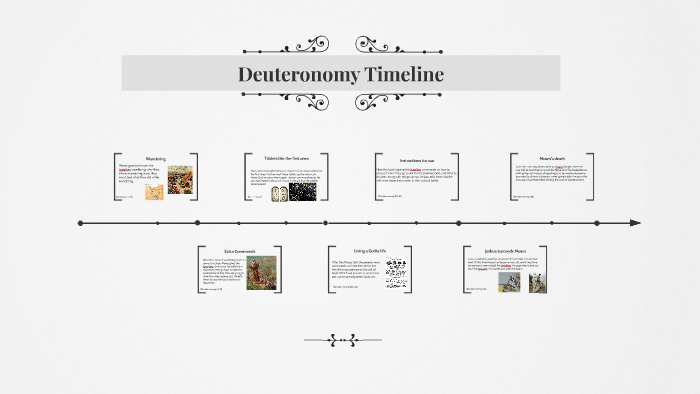
\includegraphics[scale=.7, angle=0]{05OT-Deuteronomy/References/AndrewSmithDeuteronomyTimeline.png}
%\caption[Deuteronomy Timeline by Andrew Smith]{Deuteronomy Timeline by Andrew %Smith}
%\label{fig:Deuteronomy Timeline by Andrew Smith}
%\end{center}
%\end{figure}

\newpage
\begin{figure}
\begin{center}
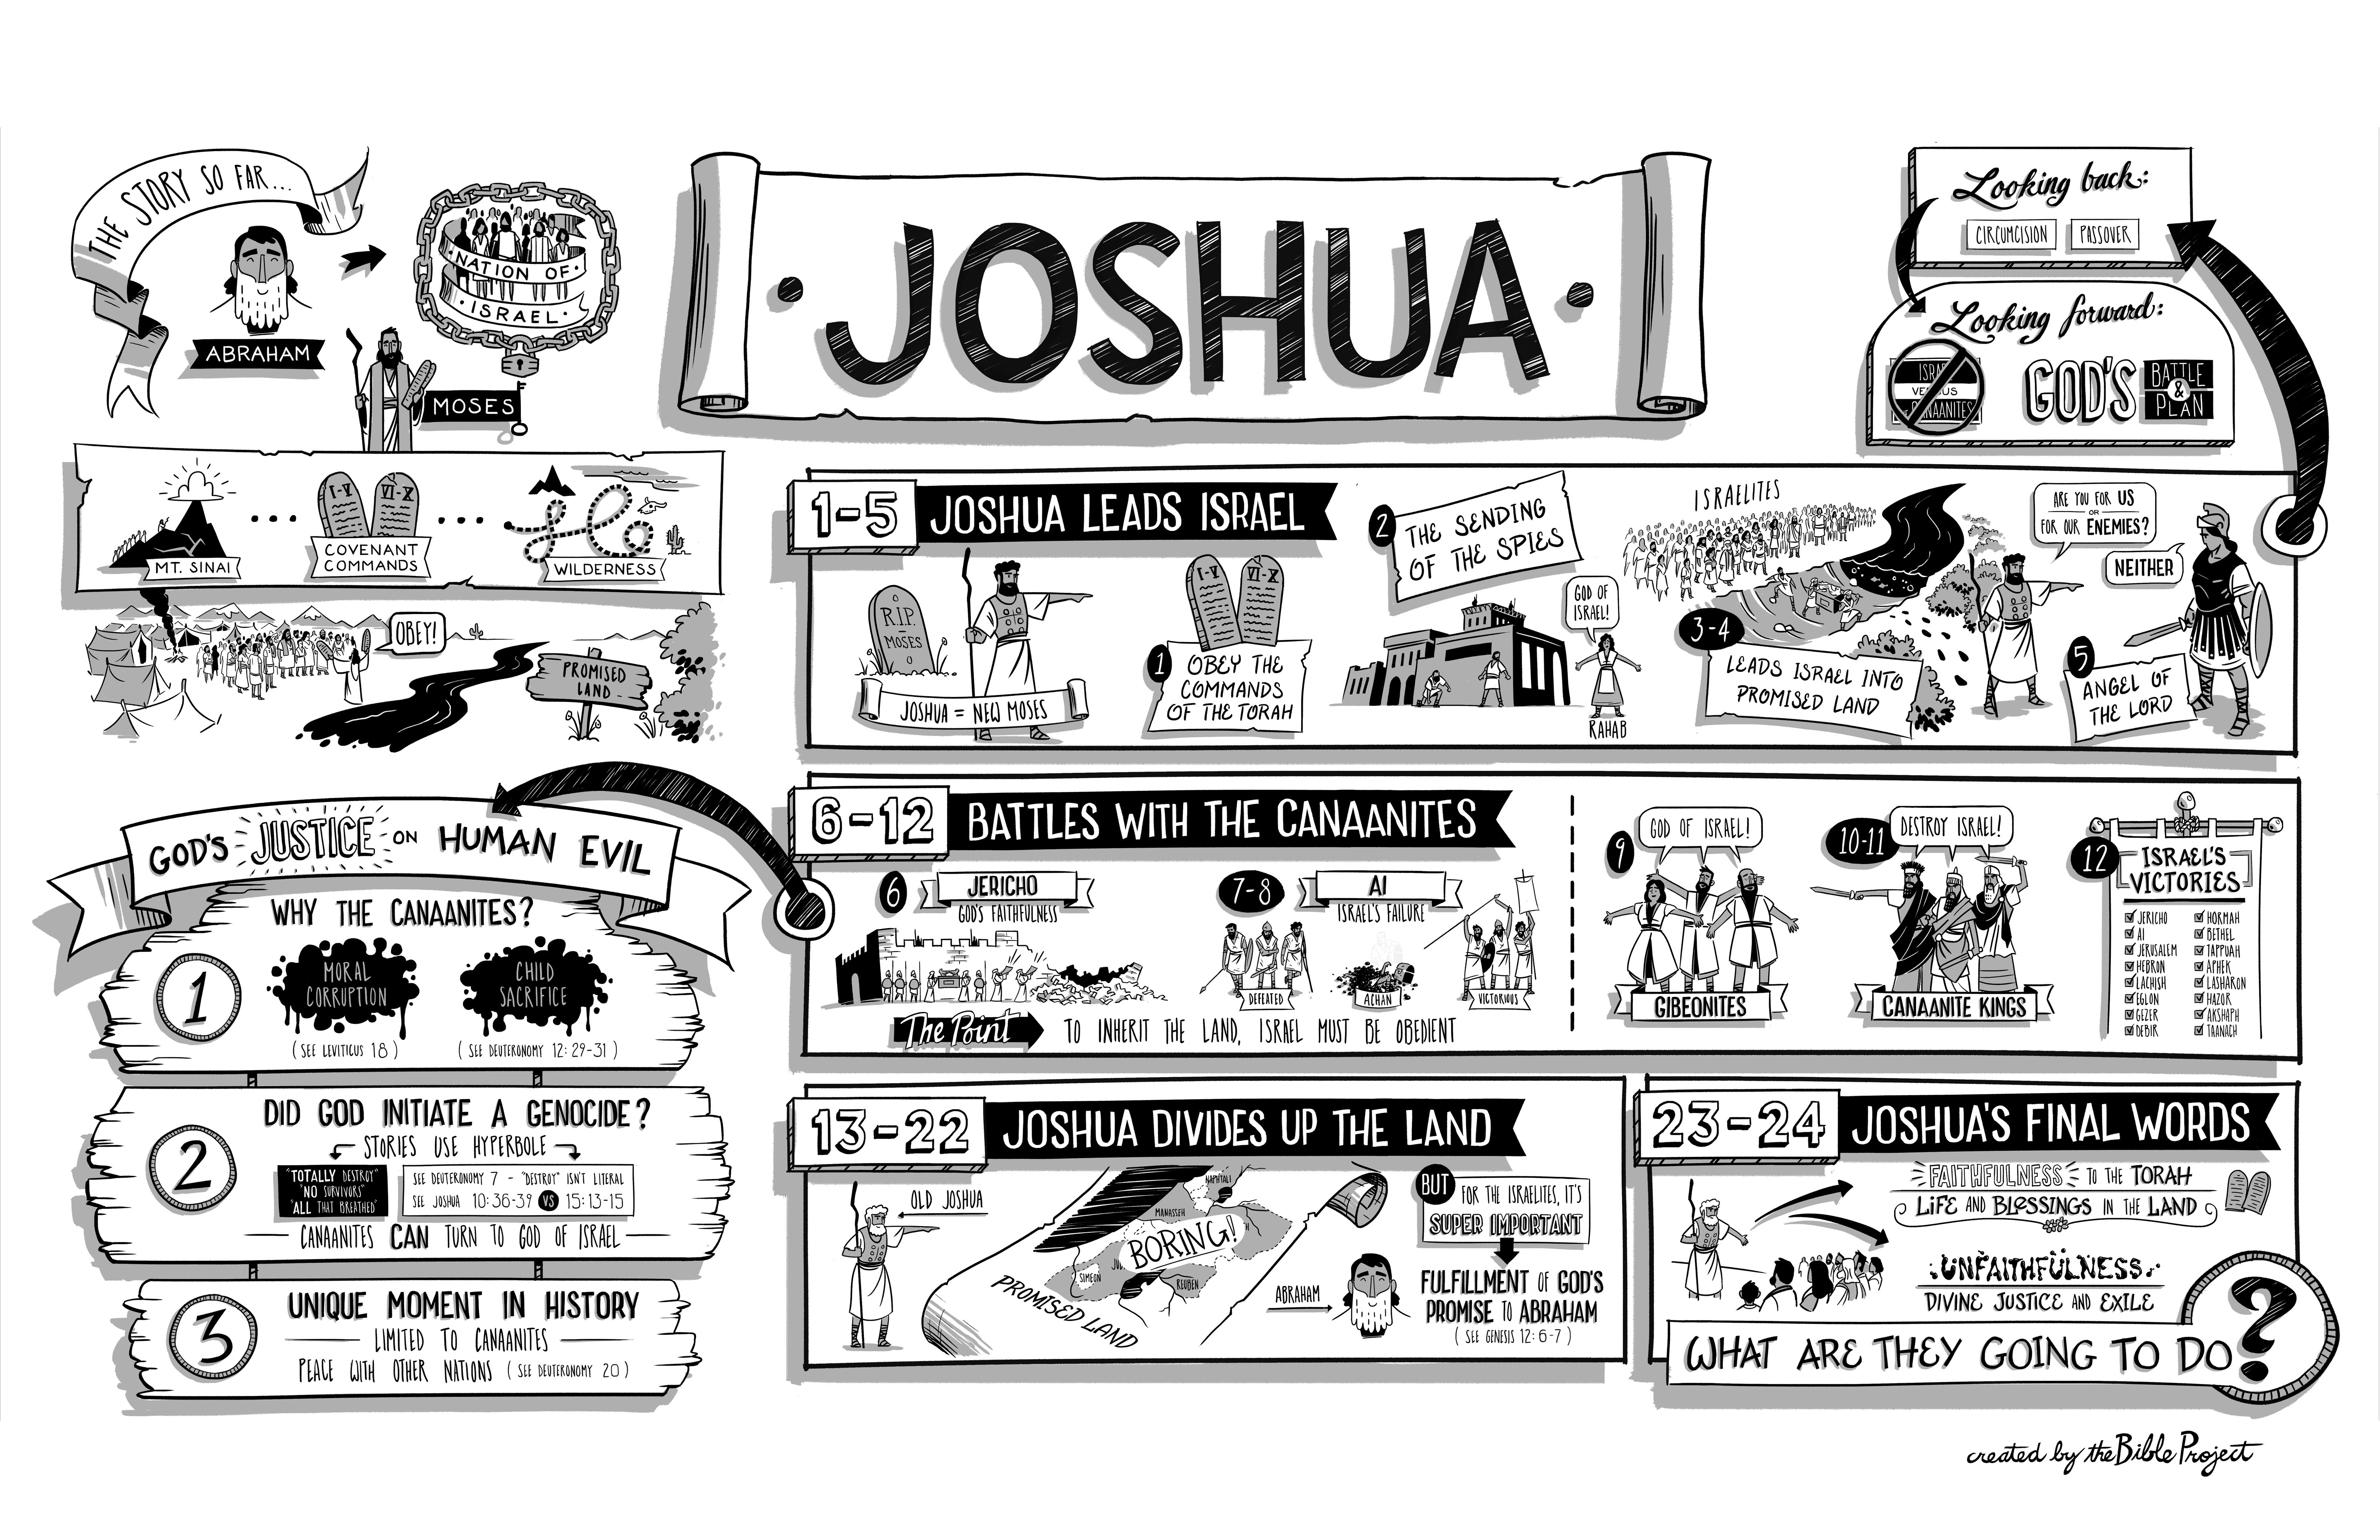
\includegraphics[scale=0.5, angle=90]{06OT-Joshua/References/1.BibleProject-Joshua.jpg}
\caption[Joshua from the Bible Project]{Joshua from the Bible Project}
\label{fig:Joshua from the Bible Project}
\end{center}
\end{figure}

\newpage
\begin{figure}
\begin{center}
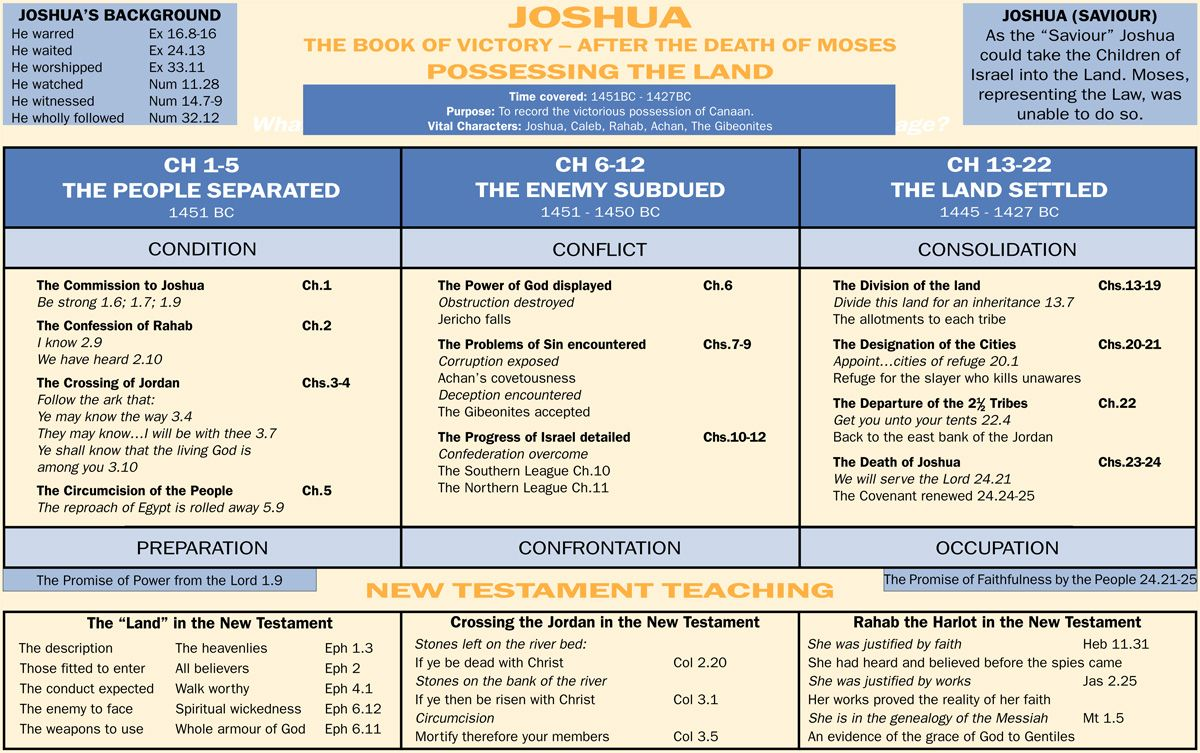
\includegraphics[scale=0.5, angle=90]{06OT-Joshua/References/2.JohnGrant-Joshua.jpg}
\caption[Joshua from John Grant]{Joshua from John Grant}
\label{fig:Joshua from John Grant}
\end{center}
\end{figure}

\newpage
\begin{figure}
\begin{center}
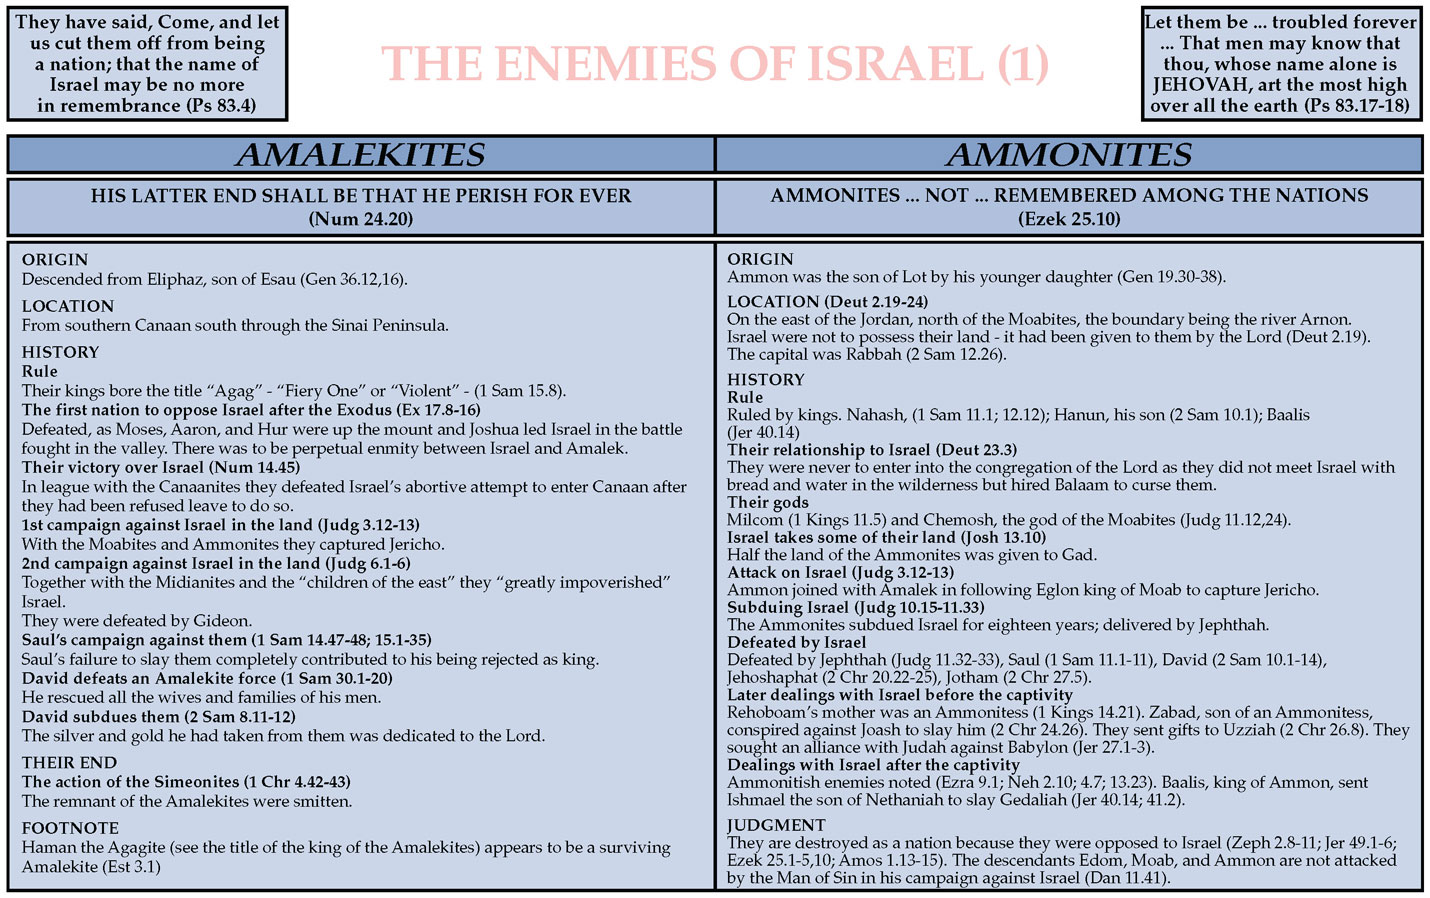
\includegraphics[scale=0.4, angle=90]{06OT-Joshua/References/3.EnemiesOfIsrael1.jpg}
\caption[Enemies of Israel 1]{Enemies of Israel 1}
\label{fig:Enemies of Israel 1}
\end{center}
\end{figure}

\newpage
\begin{figure}
\begin{center}
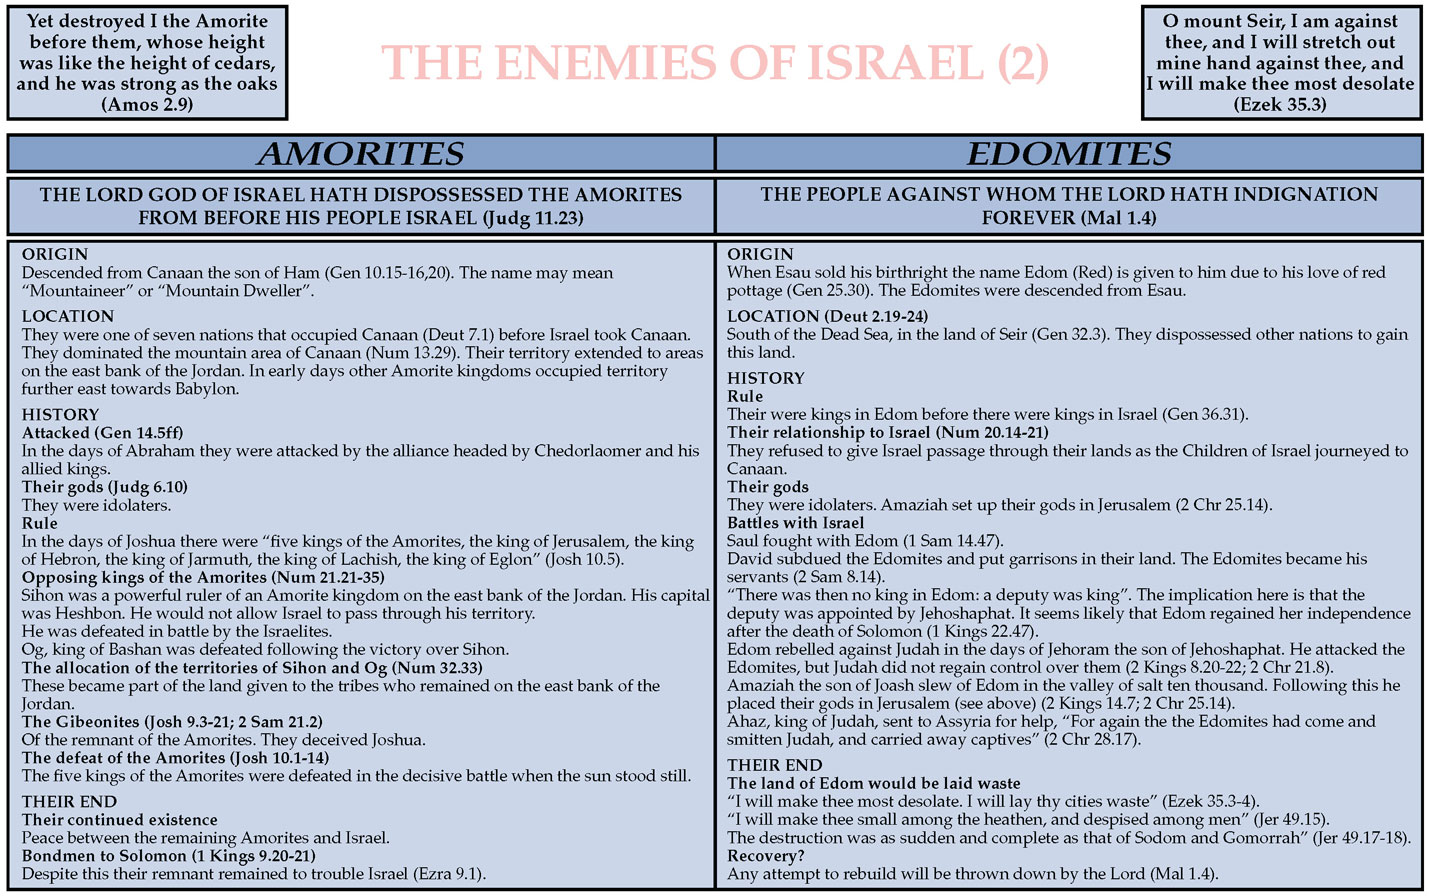
\includegraphics[scale=0.4, angle=90]{06OT-Joshua/References/4.EnemiesOfIsrael2.jpg}
\caption[Enemies of Israel 2]{Enemies of Israel 2}
\label{fig:Enemies of Israel 2}
\end{center}
\end{figure}

\newpage
\begin{figure}
\begin{center}
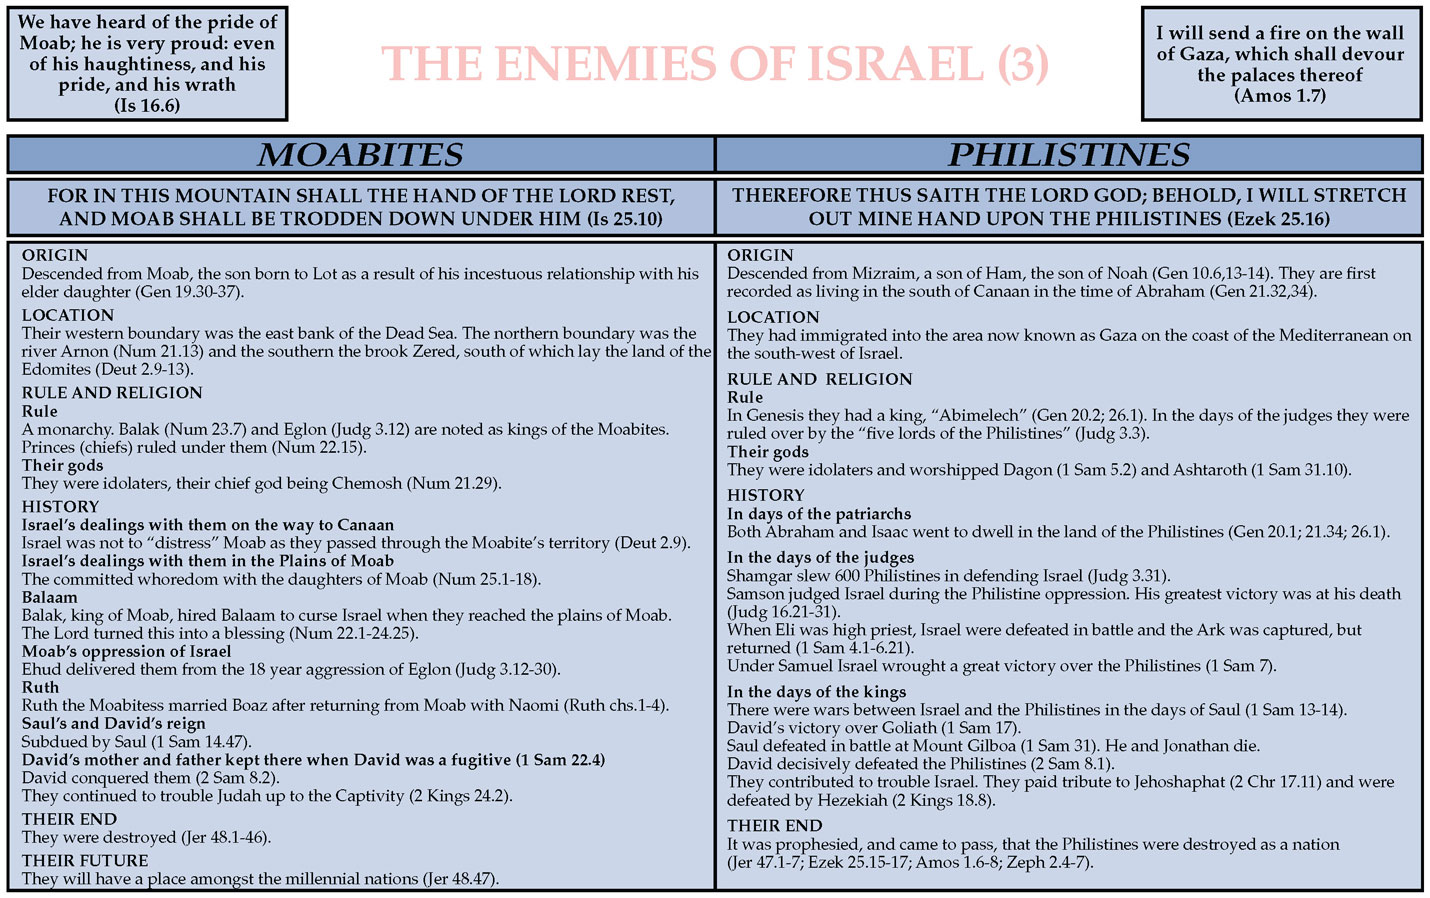
\includegraphics[scale=0.4, angle=90]{06OT-Joshua/References/5.EnemiesOfIsrael3.jpg}
\caption[Enemies of Israel 3]{Enemies of Israel 3}
\label{fig:Enemies of Israel 3}
\end{center}
\end{figure}

\newpage
\begin{figure}
\begin{center}
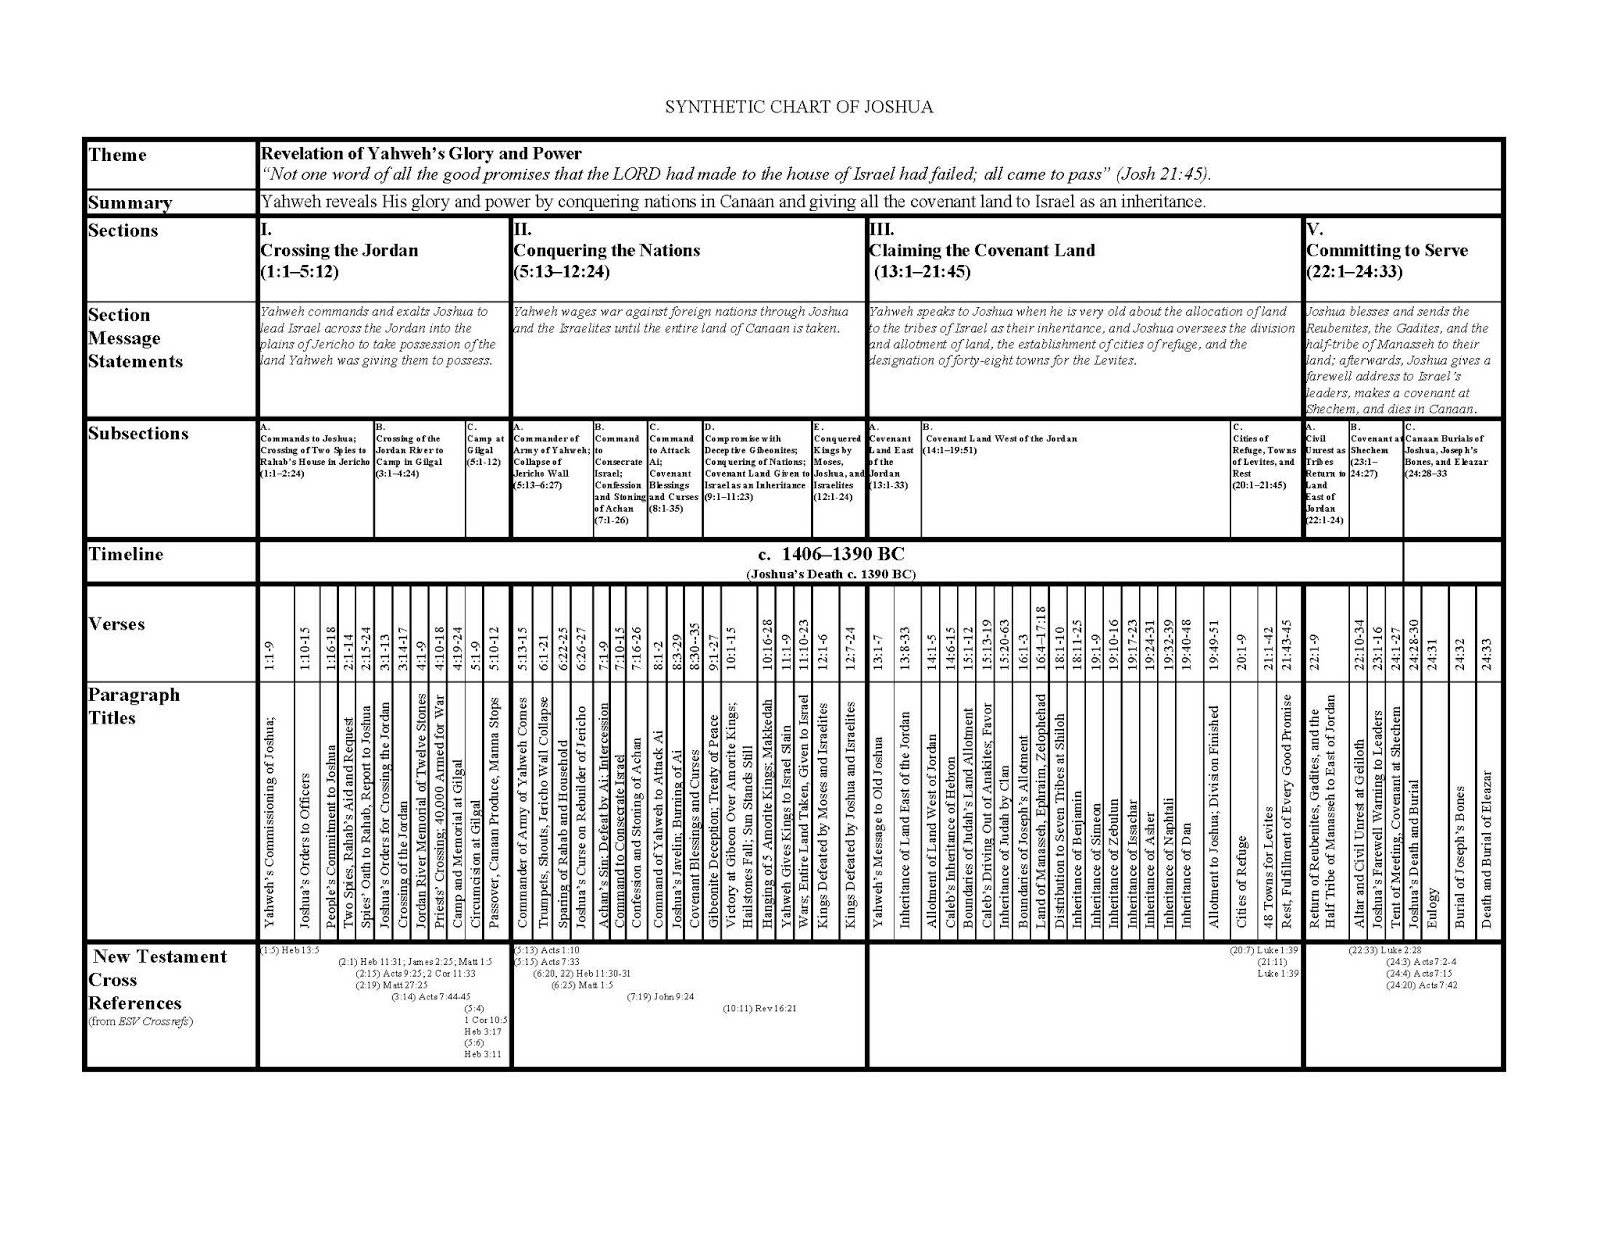
\includegraphics[scale=.4, angle=90]{06OT-Joshua/References/6.SyntheticChartofJoshua.jpg}
\caption[Synthetic Chart of Joshua]{Synthetic Chart of Joshua}
\label{fig:Synthetic Chart of Joshua}
\end{center}
\end{figure}


\newpage
\begin{figure}
\begin{center}
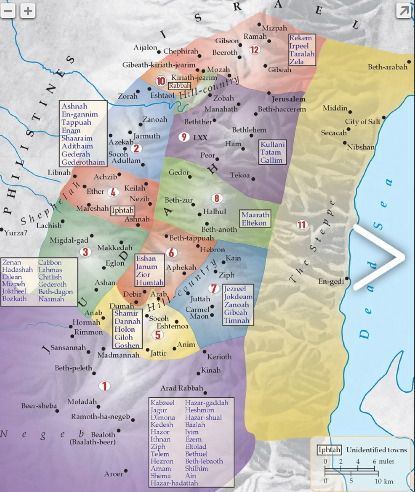
\includegraphics[scale=1, angle=0]{06OT-Joshua/References/7.WestSideOfDeadSea.jpg}
\caption[The West Side of the Dead Sea]{The West Side of the Dead Sea}
\label{fig:The West Side of the Dead Sea}
\end{center}
\end{figure}


\newpage
\begin{figure}
\begin{center}
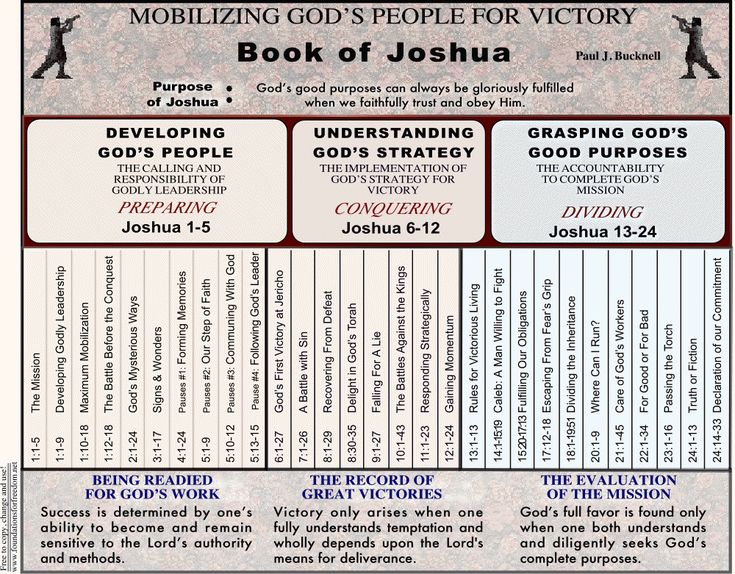
\includegraphics[scale=0.75, angle=90]{06OT-Joshua/References/8.Bucknell-Joshua.jpg}
\caption[Joshua from Bucknell]{Joshua from Bucknell}
\label{fig:Joshua from Bucknell}
\end{center}
\end{figure}


\newpage
\begin{figure}
\begin{center}
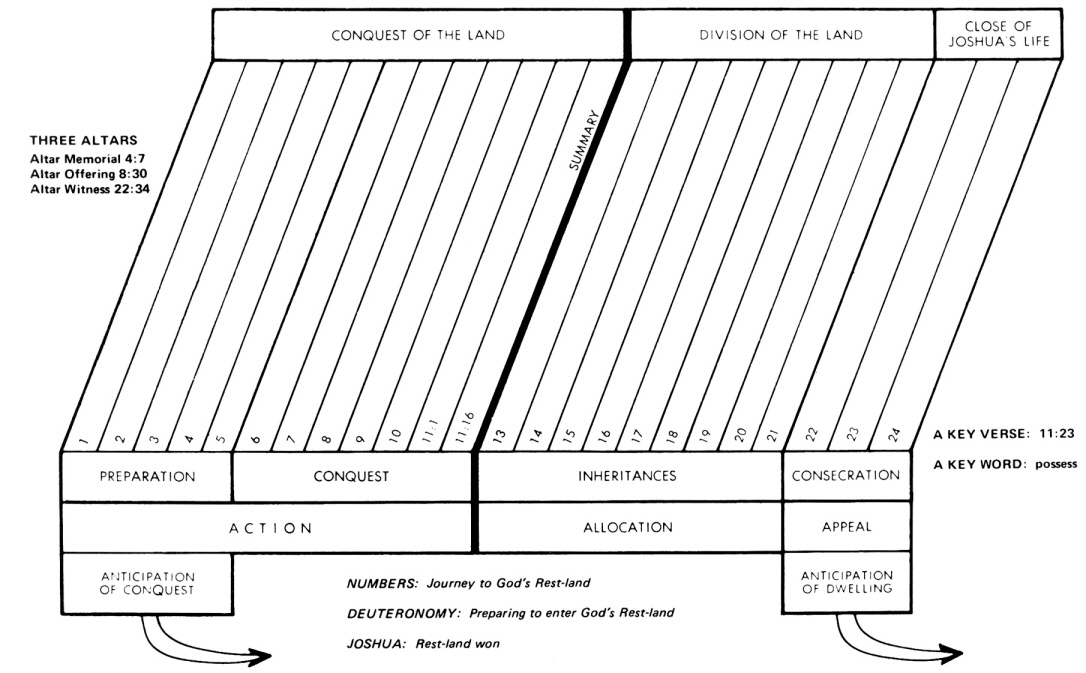
\includegraphics[scale=2, angle=90]{06OT-Joshua/References/9.Jensen-Joshua.png}
\caption[Joshua from Jensen]{Joshua from Jensen}
\label{fig:Joshua from Jensen}
\end{center}
\end{figure}


\newpage
\begin{figure}
\begin{center}
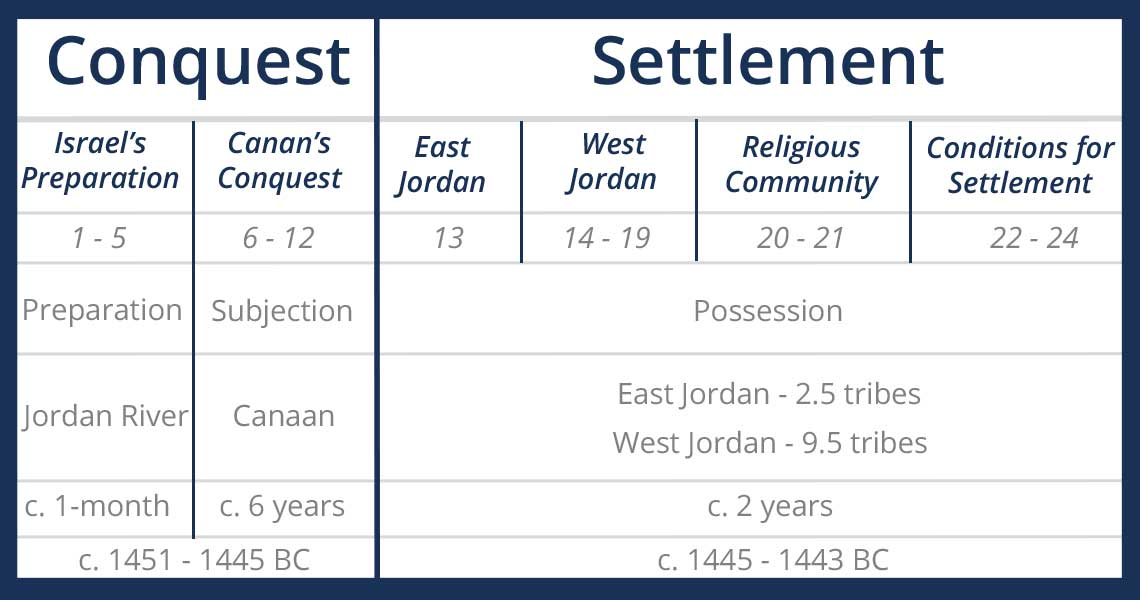
\includegraphics[scale=.5, angle=90]{06OT-Joshua/References/10.Bible-Brief-Joshua.jpg}
\caption[Bible Brief for Joshua]{Bible Brief for Joshua}
\label{fig:Bible Brief for Joshua}
\end{center}
\end{figure}

\newpage
\begin{figure}
\begin{center}
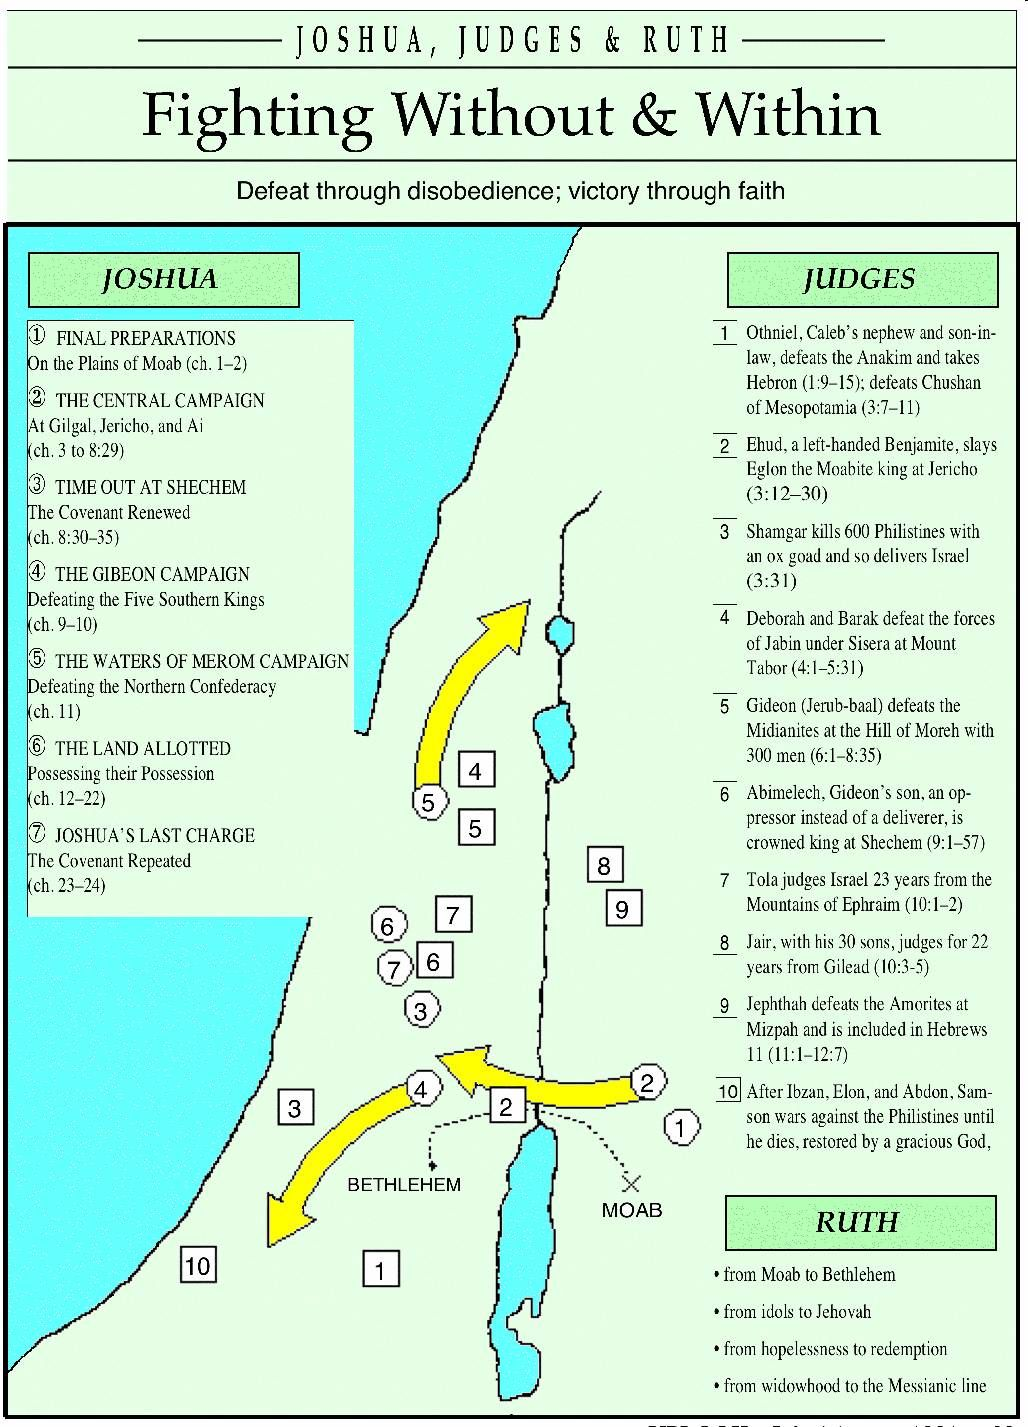
\includegraphics[scale=.5, angle=0]{06OT-Joshua/References/11.FightingInJoshuaAndJudges.jpg}
\caption[The Fighting in Joshua and Judges]{The Fighting in Joshua and Judges}
\label{fig:The Fighting in Joshua and Judges}
\end{center}
\end{figure}

\newpage
\begin{figure}
\begin{center}
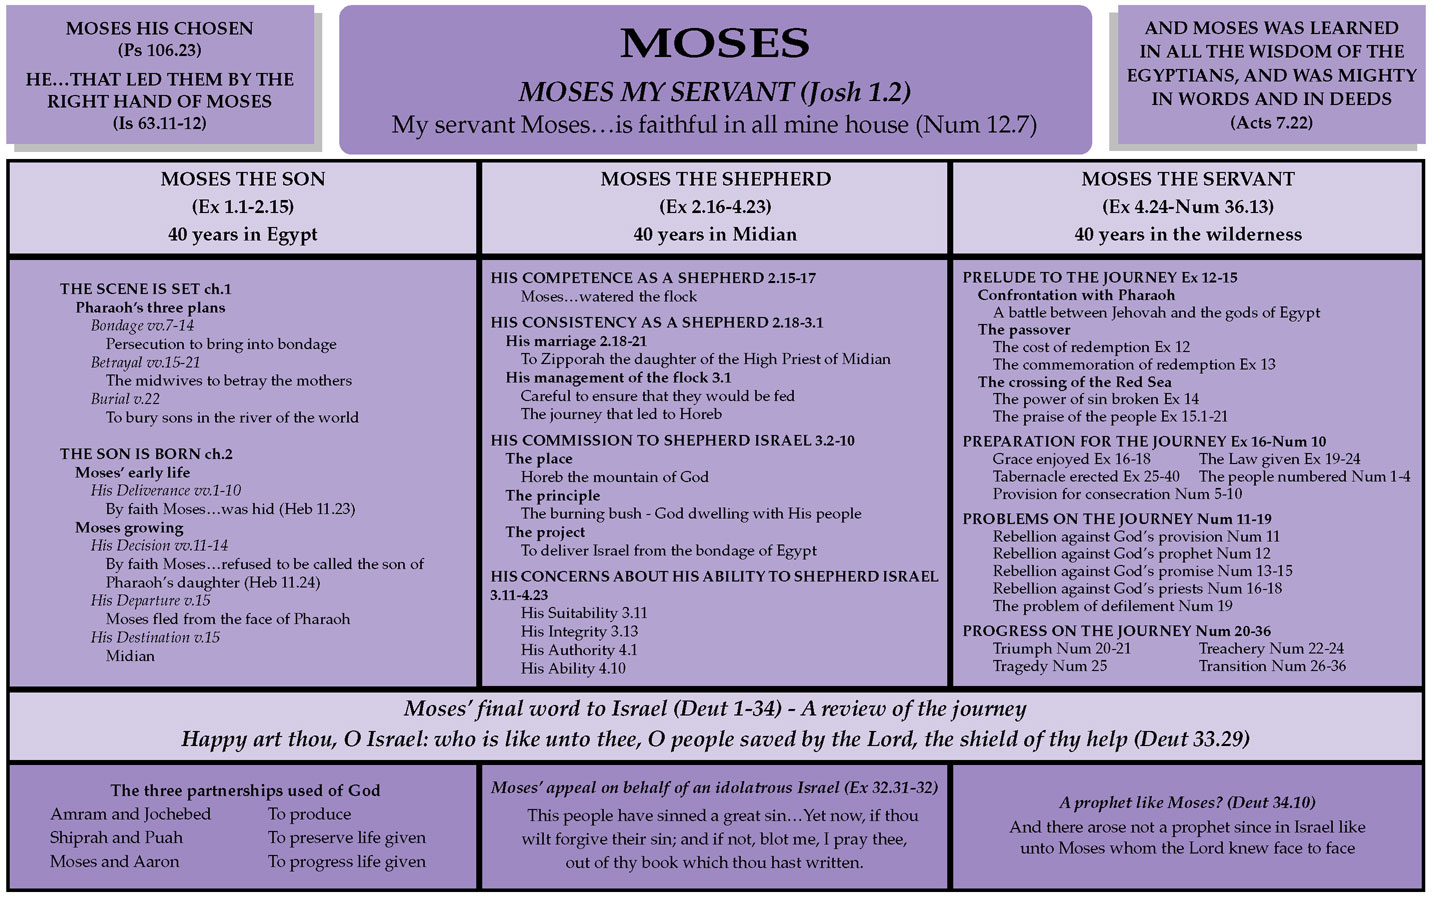
\includegraphics[scale=.4, angle=90]{06OT-Joshua/References/12.JohnGrantMoses.jpg}
\caption[Moses from John Grant]{Moses from John Grant}
\label{fig:Moses from John Grant}
\end{center}
\end{figure}








\chapter{Joshua 4}

\begin{figure}
  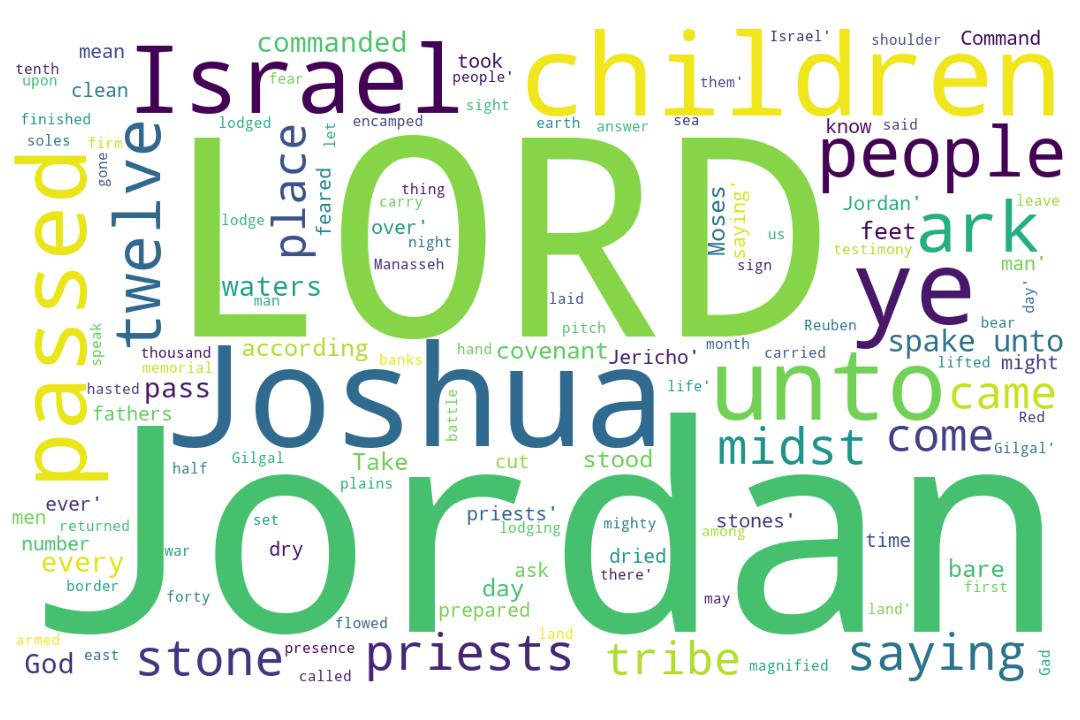
\includegraphics[width=\linewidth]{06OT-Joshua/Joshua4-WordCloud.jpg}
  \caption{Joshua 4 Word Cloud}
  \label{fig:Joshua 4 Word Cloud}
\end{figure}


\marginpar{\scriptsize \centering \fcolorbox{bone}{lime}{\textbf{TWELVE STONES}}\\ (Joshua 4:1-24)

\begin{compactenum}[I.][8]
    \item   \textbf{Truth Spoken}  \index[scripture]{Joshua!Jsh 04:01}\index[scripture]{Joshua!Jsh 04:08}\index[scripture]{Joshua!Jsh 04:12}\index[scripture]{Joshua!Jsh 04:15}\index[scripture]{Joshua!Jsh 04:21}   (Jsh 4:1, 8, 10, 12, 15, 21) 
    \item  \textbf{Twelve Stones} \index[scripture]{Joshua!Jsh 04:03}  \index[scripture]{Joshua!Jsh 04:06}  \index[scripture]{Joshua!Jsh 04:07}  \index[scripture]{Joshua!Jsh 04:08}  \index[scripture]{Joshua!Jsh 04:09}  \index[scripture]{Joshua!Jsh 04:20}  \index[scripture]{Joshua!Jsh 04:21}   (Jsh 4:3, 6, 7, 8, 9, 20, 21) 
    \item   \textbf{Torchbearers Standing}  \index[scripture]{Joshua!Jsh 04:03}\index[scripture]{Joshua!Jsh 04:09}\index[scripture]{Joshua!Jsh 04:10}   (Jsh 4:3, 9, 10) 
    \item   \textbf{Twelve Shoulders}  \index[scripture]{Joshua!Jsh 04:05}   (Jsh 4:5) 
    \item  Something \textbf{Truly Supernatural} \index[scripture]{Joshua!Jsh 04:10}   (Jsh 4:10)
    \item   \textbf{Testimony seen}  \index[scripture]{Joshua!Jsh 04:19}\index[scripture]{Joshua!Jsh 04:20}   (Jsh 4:19, 20) 
    \item A  \textbf{Theme in Scripture}  \index[scripture]{Joshua!Jsh 04:21}   (Jsh 4:3, 6, 7, 8, 9, 20, 21) 
\end{compactenum}}


\footnote{\textcolor[cmyk]{0.99998,1,0,0}{\hyperlink{TOC}{Return to end of Table of Contents.}}}\footnote{\href{https://audiobible.com/bible/joshua_4.html}{\textcolor[cmyk]{0.99998,1,0,0}{Joshua 4 Audio}}}\textcolor[cmyk]{0.99998,1,0,0}{And it came to pass, when all the people were clean passed over Jordan, that the \fcolorbox{bone}{lime}{LORD spake} unto Joshua, saying,}
[2] \textcolor[cmyk]{0.99998,1,0,0}{Take you twelve men out of the people, out of every tribe a man,}
[3] \textcolor[cmyk]{0.99998,1,0,0}{And command ye them, saying, Take you hence out of the midst of Jordan, out of the place where the priests' feet stood firm, twelve stones, and ye shall carry them over with you, and leave them in the lodging place, where ye shall lodge this night.}
[4] \textcolor[cmyk]{0.99998,1,0,0}{Then Joshua called the twelve men, whom he had prepared of the children of Israel, out of every tribe a man:}
[5] \textcolor[cmyk]{0.99998,1,0,0}{And Joshua said unto them, Pass over before the ark of the LORD your God into the midst of Jordan, and take ye up every man of you a stone upon his \fcolorbox{bone}{lime}{shoulder}, according unto the number of the tribes of the children of Israel:}
[6] \textcolor[cmyk]{0.99998,1,0,0}{That this may be a sign among you, \emph{that} when your children ask \emph{their} \emph{fathers} in time to come, saying, What \emph{mean} ye by these stones?}
[7] \textcolor[cmyk]{0.99998,1,0,0}{Then ye shall answer them, That the waters of Jordan were cut off before the ark of the covenant of the LORD; when it passed over Jordan, the waters of Jordan were cut off: and these stones shall be for a memorial unto the children of Israel for ever.}
[8] \textcolor[cmyk]{0.99998,1,0,0}{And the children of Israel did so as Joshua commanded, and took up twelve stones out of the midst of Jordan, as the \fcolorbox{bone}{lime}{LORD spake} unto Joshua, according to the number of the tribes of the children of Israel, and carried them over with them unto the place where they lodged, and laid them down there.}
[9] \textcolor[cmyk]{0.99998,1,0,0}{And Joshua set up twelve stones in the midst of Jordan, in the place where the feet of the priests which bare the ark of the covenant stood: and they are there unto this day.}\\
\\
\P \textcolor[cmyk]{0.99998,1,0,0}{For the priests which bare the ark stood in the midst of Jordan, until every thing was finished that the \fcolorbox{bone}{lime}{LORD commanded} Joshua to speak unto the people, according to all that Moses commanded Joshua: and the people hasted and passed over.}
[11] \textcolor[cmyk]{0.99998,1,0,0}{And it came to pass, when all the people were clean passed over, that the ark of the LORD passed over, and the priests, in the presence of the people.}
[12] \textcolor[cmyk]{0.99998,1,0,0}{And the children of Reuben, and the children of Gad, and half the tribe of Manasseh, passed over armed before the children of Israel, as \fcolorbox{bone}{lime}{Moses spake} unto them:}
[13] \textcolor[cmyk]{0.99998,1,0,0}{About forty thousand prepared for war passed over before the LORD unto battle, to the plains of Jericho.}\\
\\
\P \textcolor[cmyk]{0.99998,1,0,0}{On that day the LORD magnified Joshua in the sight of all Israel; and they feared him, as they feared Moses, all the days of his life.}
[15] \textcolor[cmyk]{0.99998,1,0,0}{And the \fcolorbox{bone}{lime}{LORD spake} unto Joshua, saying,}
[16] \textcolor[cmyk]{0.99998,1,0,0}{Command the priests that bear the ark of the testimony, that they come up out of Jordan.}
[17] \textcolor[cmyk]{0.99998,1,0,0}{Joshua therefore commanded the priests, saying, Come ye up out of Jordan.}
[18] \textcolor[cmyk]{0.99998,1,0,0}{And it came to pass, when the priests that bare the ark of the covenant of the LORD were come up out of the midst of Jordan, \emph{and} the soles of the priests' feet were lifted up unto the dry land, that the waters of Jordan returned unto their place, and flowed over all his banks, as \emph{they} \emph{did} before.}\\
\\
\P \textcolor[cmyk]{0.99998,1,0,0}{And the people came up out of Jordan on the tenth \emph{day} of the first month, and encamped in Gilgal, in the east border of Jericho.}
[20] \textcolor[cmyk]{0.99998,1,0,0}{And those twelve stones, which they took out of Jordan, did Joshua pitch in Gilgal.}
[21] \textcolor[cmyk]{0.99998,1,0,0}{And he \fcolorbox{bone}{lime}{spake} unto the children of Israel, saying, When your children shall ask their fathers in time to come, saying, What \emph{mean} these stones?}
[22] \textcolor[cmyk]{0.99998,1,0,0}{Then ye shall let your children know, saying, Israel came over this Jordan on dry land.}
[23] \textcolor[cmyk]{0.99998,1,0,0}{For the LORD your God dried up the waters of Jordan from before you, until ye were passed over, as the LORD your God did to the Red sea, which he dried up from before us, until we were gone over:}
[24] \textcolor[cmyk]{0.99998,1,0,0}{That all the people of the earth might know the hand of the LORD, that it \emph{is} mighty: that ye might fear the LORD your God for ever.}
\index[NWIV]{21!Joshua!Jos 4:1}\index[AWIP]{And!Joshua!Jos 4:1}\index[AWIP]{it!Joshua!Jos 4:1}\index[AWIP]{came!Joshua!Jos 4:1}\index[AWIP]{to!Joshua!Jos 4:1}\index[AWIP]{pass!Joshua!Jos 4:1}\index[AWIP]{when!Joshua!Jos 4:1}\index[AWIP]{all!Joshua!Jos 4:1}\index[AWIP]{the!Joshua!Jos 4:1}\index[AWIP]{the!Joshua!Jos 4:1 (2)}\index[AWIP]{people!Joshua!Jos 4:1}\index[AWIP]{were!Joshua!Jos 4:1}\index[AWIP]{clean!Joshua!Jos 4:1}\index[AWIP]{passed!Joshua!Jos 4:1}\index[AWIP]{over!Joshua!Jos 4:1}\index[AWIP]{Jordan!Joshua!Jos 4:1}\index[AWIP]{that!Joshua!Jos 4:1}\index[AWIP]{LORD!Joshua!Jos 4:1}\index[AWIP]{spake!Joshua!Jos 4:1}\index[AWIP]{unto!Joshua!Jos 4:1}\index[AWIP]{Joshua!Joshua!Jos 4:1}\index[AWIP]{saying!Joshua!Jos 4:1}

\index[NWIV]{14!Joshua!Jos 4:2}\index[AWIP]{Take!Joshua!Jos 4:2}\index[AWIP]{you!Joshua!Jos 4:2}\index[AWIP]{twelve!Joshua!Jos 4:2}\index[AWIP]{men!Joshua!Jos 4:2}\index[AWIP]{out!Joshua!Jos 4:2}\index[AWIP]{out!Joshua!Jos 4:2 (2)}\index[AWIP]{of!Joshua!Jos 4:2}\index[AWIP]{of!Joshua!Jos 4:2 (2)}\index[AWIP]{the!Joshua!Jos 4:2}\index[AWIP]{people!Joshua!Jos 4:2}\index[AWIP]{every!Joshua!Jos 4:2}\index[AWIP]{tribe!Joshua!Jos 4:2}\index[AWIP]{a!Joshua!Jos 4:2}\index[AWIP]{man!Joshua!Jos 4:2}

\index[NWIV]{47!Joshua!Jos 4:3}\index[AWIP]{And!Joshua!Jos 4:3}\index[AWIP]{command!Joshua!Jos 4:3}\index[AWIP]{ye!Joshua!Jos 4:3}\index[AWIP]{ye!Joshua!Jos 4:3 (2)}\index[AWIP]{ye!Joshua!Jos 4:3 (3)}\index[AWIP]{them!Joshua!Jos 4:3}\index[AWIP]{them!Joshua!Jos 4:3 (2)}\index[AWIP]{them!Joshua!Jos 4:3 (3)}\index[AWIP]{saying!Joshua!Jos 4:3}\index[AWIP]{Take!Joshua!Jos 4:3}\index[AWIP]{you!Joshua!Jos 4:3}\index[AWIP]{you!Joshua!Jos 4:3 (2)}\index[AWIP]{hence!Joshua!Jos 4:3}\index[AWIP]{out!Joshua!Jos 4:3}\index[AWIP]{out!Joshua!Jos 4:3 (2)}\index[AWIP]{of!Joshua!Jos 4:3}\index[AWIP]{of!Joshua!Jos 4:3 (2)}\index[AWIP]{of!Joshua!Jos 4:3 (3)}\index[AWIP]{the!Joshua!Jos 4:3}\index[AWIP]{the!Joshua!Jos 4:3 (2)}\index[AWIP]{the!Joshua!Jos 4:3 (3)}\index[AWIP]{the!Joshua!Jos 4:3 (4)}\index[AWIP]{midst!Joshua!Jos 4:3}\index[AWIP]{Jordan!Joshua!Jos 4:3}\index[AWIP]{place!Joshua!Jos 4:3}\index[AWIP]{place!Joshua!Jos 4:3 (2)}\index[AWIP]{where!Joshua!Jos 4:3}\index[AWIP]{where!Joshua!Jos 4:3 (2)}\index[AWIP]{priests'!Joshua!Jos 4:3}\index[AWIP]{feet!Joshua!Jos 4:3}\index[AWIP]{stood!Joshua!Jos 4:3}\index[AWIP]{firm!Joshua!Jos 4:3}\index[AWIP]{twelve!Joshua!Jos 4:3}\index[AWIP]{stones!Joshua!Jos 4:3}\index[AWIP]{and!Joshua!Jos 4:3}\index[AWIP]{and!Joshua!Jos 4:3 (2)}\index[AWIP]{shall!Joshua!Jos 4:3}\index[AWIP]{shall!Joshua!Jos 4:3 (2)}\index[AWIP]{carry!Joshua!Jos 4:3}\index[AWIP]{over!Joshua!Jos 4:3}\index[AWIP]{with!Joshua!Jos 4:3}\index[AWIP]{leave!Joshua!Jos 4:3}\index[AWIP]{in!Joshua!Jos 4:3}\index[AWIP]{lodging!Joshua!Jos 4:3}\index[AWIP]{lodge!Joshua!Jos 4:3}\index[AWIP]{this!Joshua!Jos 4:3}\index[AWIP]{night!Joshua!Jos 4:3}

\index[NWIV]{21!Joshua!Jos 4:4}\index[AWIP]{Then!Joshua!Jos 4:4}\index[AWIP]{Joshua!Joshua!Jos 4:4}\index[AWIP]{called!Joshua!Jos 4:4}\index[AWIP]{the!Joshua!Jos 4:4}\index[AWIP]{the!Joshua!Jos 4:4 (2)}\index[AWIP]{twelve!Joshua!Jos 4:4}\index[AWIP]{men!Joshua!Jos 4:4}\index[AWIP]{whom!Joshua!Jos 4:4}\index[AWIP]{he!Joshua!Jos 4:4}\index[AWIP]{had!Joshua!Jos 4:4}\index[AWIP]{prepared!Joshua!Jos 4:4}\index[AWIP]{of!Joshua!Jos 4:4}\index[AWIP]{of!Joshua!Jos 4:4 (2)}\index[AWIP]{of!Joshua!Jos 4:4 (3)}\index[AWIP]{children!Joshua!Jos 4:4}\index[AWIP]{Israel!Joshua!Jos 4:4}\index[AWIP]{out!Joshua!Jos 4:4}\index[AWIP]{every!Joshua!Jos 4:4}\index[AWIP]{tribe!Joshua!Jos 4:4}\index[AWIP]{a!Joshua!Jos 4:4}\index[AWIP]{man!Joshua!Jos 4:4}

\index[NWIV]{45!Joshua!Jos 4:5}\index[AWIP]{And!Joshua!Jos 4:5}\index[AWIP]{Joshua!Joshua!Jos 4:5}\index[AWIP]{said!Joshua!Jos 4:5}\index[AWIP]{unto!Joshua!Jos 4:5}\index[AWIP]{unto!Joshua!Jos 4:5 (2)}\index[AWIP]{them!Joshua!Jos 4:5}\index[AWIP]{Pass!Joshua!Jos 4:5}\index[AWIP]{over!Joshua!Jos 4:5}\index[AWIP]{before!Joshua!Jos 4:5}\index[AWIP]{the!Joshua!Jos 4:5}\index[AWIP]{the!Joshua!Jos 4:5 (2)}\index[AWIP]{the!Joshua!Jos 4:5 (3)}\index[AWIP]{the!Joshua!Jos 4:5 (4)}\index[AWIP]{the!Joshua!Jos 4:5 (5)}\index[AWIP]{the!Joshua!Jos 4:5 (6)}\index[AWIP]{ark!Joshua!Jos 4:5}\index[AWIP]{of!Joshua!Jos 4:5}\index[AWIP]{of!Joshua!Jos 4:5 (2)}\index[AWIP]{of!Joshua!Jos 4:5 (3)}\index[AWIP]{of!Joshua!Jos 4:5 (4)}\index[AWIP]{of!Joshua!Jos 4:5 (5)}\index[AWIP]{of!Joshua!Jos 4:5 (6)}\index[AWIP]{LORD!Joshua!Jos 4:5}\index[AWIP]{your!Joshua!Jos 4:5}\index[AWIP]{God!Joshua!Jos 4:5}\index[AWIP]{into!Joshua!Jos 4:5}\index[AWIP]{midst!Joshua!Jos 4:5}\index[AWIP]{Jordan!Joshua!Jos 4:5}\index[AWIP]{and!Joshua!Jos 4:5}\index[AWIP]{take!Joshua!Jos 4:5}\index[AWIP]{ye!Joshua!Jos 4:5}\index[AWIP]{up!Joshua!Jos 4:5}\index[AWIP]{every!Joshua!Jos 4:5}\index[AWIP]{man!Joshua!Jos 4:5}\index[AWIP]{you!Joshua!Jos 4:5}\index[AWIP]{a!Joshua!Jos 4:5}\index[AWIP]{stone!Joshua!Jos 4:5}\index[AWIP]{upon!Joshua!Jos 4:5}\index[AWIP]{his!Joshua!Jos 4:5}\index[AWIP]{shoulder!Joshua!Jos 4:5}\index[AWIP]{according!Joshua!Jos 4:5}\index[AWIP]{number!Joshua!Jos 4:5}\index[AWIP]{tribes!Joshua!Jos 4:5}\index[AWIP]{children!Joshua!Jos 4:5}\index[AWIP]{Israel!Joshua!Jos 4:5}

\index[NWIV]{26!Joshua!Jos 4:6}\index[AWIP]{That!Joshua!Jos 4:6}\index[AWIP]{this!Joshua!Jos 4:6}\index[AWIP]{may!Joshua!Jos 4:6}\index[AWIP]{be!Joshua!Jos 4:6}\index[AWIP]{a!Joshua!Jos 4:6}\index[AWIP]{sign!Joshua!Jos 4:6}\index[AWIP]{among!Joshua!Jos 4:6}\index[AWIP]{you!Joshua!Jos 4:6}\index[AWIP]{\emph{that}!Joshua!Jos 4:6}\index[AWIP]{when!Joshua!Jos 4:6}\index[AWIP]{your!Joshua!Jos 4:6}\index[AWIP]{children!Joshua!Jos 4:6}\index[AWIP]{ask!Joshua!Jos 4:6}\index[AWIP]{\emph{their}!Joshua!Jos 4:6}\index[AWIP]{\emph{fathers}!Joshua!Jos 4:6}\index[AWIP]{in!Joshua!Jos 4:6}\index[AWIP]{time!Joshua!Jos 4:6}\index[AWIP]{to!Joshua!Jos 4:6}\index[AWIP]{come!Joshua!Jos 4:6}\index[AWIP]{saying!Joshua!Jos 4:6}\index[AWIP]{What!Joshua!Jos 4:6}\index[AWIP]{\emph{mean}!Joshua!Jos 4:6}\index[AWIP]{ye!Joshua!Jos 4:6}\index[AWIP]{by!Joshua!Jos 4:6}\index[AWIP]{these!Joshua!Jos 4:6}\index[AWIP]{stones!Joshua!Jos 4:6}\index[AWIP]{\emph{that}!Joshua!Jos 4:6}\index[AWIP]{\emph{their}!Joshua!Jos 4:6}\index[AWIP]{\emph{fathers}!Joshua!Jos 4:6}\index[AWIP]{\emph{mean}!Joshua!Jos 4:6}

\index[NWIV]{49!Joshua!Jos 4:7}\index[AWIP]{Then!Joshua!Jos 4:7}\index[AWIP]{ye!Joshua!Jos 4:7}\index[AWIP]{shall!Joshua!Jos 4:7}\index[AWIP]{shall!Joshua!Jos 4:7 (2)}\index[AWIP]{answer!Joshua!Jos 4:7}\index[AWIP]{them!Joshua!Jos 4:7}\index[AWIP]{That!Joshua!Jos 4:7}\index[AWIP]{the!Joshua!Jos 4:7}\index[AWIP]{the!Joshua!Jos 4:7 (2)}\index[AWIP]{the!Joshua!Jos 4:7 (3)}\index[AWIP]{the!Joshua!Jos 4:7 (4)}\index[AWIP]{the!Joshua!Jos 4:7 (5)}\index[AWIP]{the!Joshua!Jos 4:7 (6)}\index[AWIP]{waters!Joshua!Jos 4:7}\index[AWIP]{waters!Joshua!Jos 4:7 (2)}\index[AWIP]{of!Joshua!Jos 4:7}\index[AWIP]{of!Joshua!Jos 4:7 (2)}\index[AWIP]{of!Joshua!Jos 4:7 (3)}\index[AWIP]{of!Joshua!Jos 4:7 (4)}\index[AWIP]{of!Joshua!Jos 4:7 (5)}\index[AWIP]{Jordan!Joshua!Jos 4:7}\index[AWIP]{Jordan!Joshua!Jos 4:7 (2)}\index[AWIP]{Jordan!Joshua!Jos 4:7 (3)}\index[AWIP]{were!Joshua!Jos 4:7}\index[AWIP]{were!Joshua!Jos 4:7 (2)}\index[AWIP]{cut!Joshua!Jos 4:7}\index[AWIP]{cut!Joshua!Jos 4:7 (2)}\index[AWIP]{off!Joshua!Jos 4:7}\index[AWIP]{off!Joshua!Jos 4:7 (2)}\index[AWIP]{before!Joshua!Jos 4:7}\index[AWIP]{ark!Joshua!Jos 4:7}\index[AWIP]{covenant!Joshua!Jos 4:7}\index[AWIP]{LORD!Joshua!Jos 4:7}\index[AWIP]{when!Joshua!Jos 4:7}\index[AWIP]{it!Joshua!Jos 4:7}\index[AWIP]{passed!Joshua!Jos 4:7}\index[AWIP]{over!Joshua!Jos 4:7}\index[AWIP]{and!Joshua!Jos 4:7}\index[AWIP]{these!Joshua!Jos 4:7}\index[AWIP]{stones!Joshua!Jos 4:7}\index[AWIP]{be!Joshua!Jos 4:7}\index[AWIP]{for!Joshua!Jos 4:7}\index[AWIP]{for!Joshua!Jos 4:7 (2)}\index[AWIP]{a!Joshua!Jos 4:7}\index[AWIP]{memorial!Joshua!Jos 4:7}\index[AWIP]{unto!Joshua!Jos 4:7}\index[AWIP]{children!Joshua!Jos 4:7}\index[AWIP]{Israel!Joshua!Jos 4:7}\index[AWIP]{ever!Joshua!Jos 4:7}

\index[NWIV]{56!Joshua!Jos 4:8}\index[AWIP]{And!Joshua!Jos 4:8}\index[AWIP]{the!Joshua!Jos 4:8}\index[AWIP]{the!Joshua!Jos 4:8 (2)}\index[AWIP]{the!Joshua!Jos 4:8 (3)}\index[AWIP]{the!Joshua!Jos 4:8 (4)}\index[AWIP]{the!Joshua!Jos 4:8 (5)}\index[AWIP]{the!Joshua!Jos 4:8 (6)}\index[AWIP]{the!Joshua!Jos 4:8 (7)}\index[AWIP]{children!Joshua!Jos 4:8}\index[AWIP]{children!Joshua!Jos 4:8 (2)}\index[AWIP]{of!Joshua!Jos 4:8}\index[AWIP]{of!Joshua!Jos 4:8 (2)}\index[AWIP]{of!Joshua!Jos 4:8 (3)}\index[AWIP]{of!Joshua!Jos 4:8 (4)}\index[AWIP]{of!Joshua!Jos 4:8 (5)}\index[AWIP]{of!Joshua!Jos 4:8 (6)}\index[AWIP]{Israel!Joshua!Jos 4:8}\index[AWIP]{Israel!Joshua!Jos 4:8 (2)}\index[AWIP]{did!Joshua!Jos 4:8}\index[AWIP]{so!Joshua!Jos 4:8}\index[AWIP]{as!Joshua!Jos 4:8}\index[AWIP]{as!Joshua!Jos 4:8 (2)}\index[AWIP]{Joshua!Joshua!Jos 4:8}\index[AWIP]{Joshua!Joshua!Jos 4:8 (2)}\index[AWIP]{commanded!Joshua!Jos 4:8}\index[AWIP]{and!Joshua!Jos 4:8}\index[AWIP]{and!Joshua!Jos 4:8 (2)}\index[AWIP]{and!Joshua!Jos 4:8 (3)}\index[AWIP]{took!Joshua!Jos 4:8}\index[AWIP]{up!Joshua!Jos 4:8}\index[AWIP]{twelve!Joshua!Jos 4:8}\index[AWIP]{stones!Joshua!Jos 4:8}\index[AWIP]{out!Joshua!Jos 4:8}\index[AWIP]{midst!Joshua!Jos 4:8}\index[AWIP]{Jordan!Joshua!Jos 4:8}\index[AWIP]{LORD!Joshua!Jos 4:8}\index[AWIP]{spake!Joshua!Jos 4:8}\index[AWIP]{unto!Joshua!Jos 4:8}\index[AWIP]{unto!Joshua!Jos 4:8 (2)}\index[AWIP]{according!Joshua!Jos 4:8}\index[AWIP]{to!Joshua!Jos 4:8}\index[AWIP]{number!Joshua!Jos 4:8}\index[AWIP]{tribes!Joshua!Jos 4:8}\index[AWIP]{carried!Joshua!Jos 4:8}\index[AWIP]{them!Joshua!Jos 4:8}\index[AWIP]{them!Joshua!Jos 4:8 (2)}\index[AWIP]{them!Joshua!Jos 4:8 (3)}\index[AWIP]{over!Joshua!Jos 4:8}\index[AWIP]{with!Joshua!Jos 4:8}\index[AWIP]{place!Joshua!Jos 4:8}\index[AWIP]{where!Joshua!Jos 4:8}\index[AWIP]{they!Joshua!Jos 4:8}\index[AWIP]{lodged!Joshua!Jos 4:8}\index[AWIP]{laid!Joshua!Jos 4:8}\index[AWIP]{down!Joshua!Jos 4:8}\index[AWIP]{there!Joshua!Jos 4:8}

\index[NWIV]{35!Joshua!Jos 4:9}\index[AWIP]{And!Joshua!Jos 4:9}\index[AWIP]{Joshua!Joshua!Jos 4:9}\index[AWIP]{set!Joshua!Jos 4:9}\index[AWIP]{up!Joshua!Jos 4:9}\index[AWIP]{twelve!Joshua!Jos 4:9}\index[AWIP]{stones!Joshua!Jos 4:9}\index[AWIP]{in!Joshua!Jos 4:9}\index[AWIP]{in!Joshua!Jos 4:9 (2)}\index[AWIP]{the!Joshua!Jos 4:9}\index[AWIP]{the!Joshua!Jos 4:9 (2)}\index[AWIP]{the!Joshua!Jos 4:9 (3)}\index[AWIP]{the!Joshua!Jos 4:9 (4)}\index[AWIP]{the!Joshua!Jos 4:9 (5)}\index[AWIP]{the!Joshua!Jos 4:9 (6)}\index[AWIP]{midst!Joshua!Jos 4:9}\index[AWIP]{of!Joshua!Jos 4:9}\index[AWIP]{of!Joshua!Jos 4:9 (2)}\index[AWIP]{of!Joshua!Jos 4:9 (3)}\index[AWIP]{Jordan!Joshua!Jos 4:9}\index[AWIP]{place!Joshua!Jos 4:9}\index[AWIP]{where!Joshua!Jos 4:9}\index[AWIP]{feet!Joshua!Jos 4:9}\index[AWIP]{priests!Joshua!Jos 4:9}\index[AWIP]{which!Joshua!Jos 4:9}\index[AWIP]{bare!Joshua!Jos 4:9}\index[AWIP]{ark!Joshua!Jos 4:9}\index[AWIP]{covenant!Joshua!Jos 4:9}\index[AWIP]{stood!Joshua!Jos 4:9}\index[AWIP]{and!Joshua!Jos 4:9}\index[AWIP]{they!Joshua!Jos 4:9}\index[AWIP]{are!Joshua!Jos 4:9}\index[AWIP]{there!Joshua!Jos 4:9}\index[AWIP]{unto!Joshua!Jos 4:9}\index[AWIP]{this!Joshua!Jos 4:9}\index[AWIP]{day!Joshua!Jos 4:9}

\index[NWIV]{42!Joshua!Jos 4:10}\index[AWIP]{For!Joshua!Jos 4:10}\index[AWIP]{the!Joshua!Jos 4:10}\index[AWIP]{the!Joshua!Jos 4:10 (2)}\index[AWIP]{the!Joshua!Jos 4:10 (3)}\index[AWIP]{the!Joshua!Jos 4:10 (4)}\index[AWIP]{the!Joshua!Jos 4:10 (5)}\index[AWIP]{the!Joshua!Jos 4:10 (6)}\index[AWIP]{priests!Joshua!Jos 4:10}\index[AWIP]{which!Joshua!Jos 4:10}\index[AWIP]{bare!Joshua!Jos 4:10}\index[AWIP]{ark!Joshua!Jos 4:10}\index[AWIP]{stood!Joshua!Jos 4:10}\index[AWIP]{in!Joshua!Jos 4:10}\index[AWIP]{midst!Joshua!Jos 4:10}\index[AWIP]{of!Joshua!Jos 4:10}\index[AWIP]{Jordan!Joshua!Jos 4:10}\index[AWIP]{until!Joshua!Jos 4:10}\index[AWIP]{every!Joshua!Jos 4:10}\index[AWIP]{thing!Joshua!Jos 4:10}\index[AWIP]{was!Joshua!Jos 4:10}\index[AWIP]{finished!Joshua!Jos 4:10}\index[AWIP]{that!Joshua!Jos 4:10}\index[AWIP]{that!Joshua!Jos 4:10 (2)}\index[AWIP]{LORD!Joshua!Jos 4:10}\index[AWIP]{commanded!Joshua!Jos 4:10}\index[AWIP]{commanded!Joshua!Jos 4:10 (2)}\index[AWIP]{Joshua!Joshua!Jos 4:10}\index[AWIP]{Joshua!Joshua!Jos 4:10 (2)}\index[AWIP]{to!Joshua!Jos 4:10}\index[AWIP]{to!Joshua!Jos 4:10 (2)}\index[AWIP]{speak!Joshua!Jos 4:10}\index[AWIP]{unto!Joshua!Jos 4:10}\index[AWIP]{people!Joshua!Jos 4:10}\index[AWIP]{people!Joshua!Jos 4:10 (2)}\index[AWIP]{according!Joshua!Jos 4:10}\index[AWIP]{all!Joshua!Jos 4:10}\index[AWIP]{Moses!Joshua!Jos 4:10}\index[AWIP]{and!Joshua!Jos 4:10}\index[AWIP]{and!Joshua!Jos 4:10 (2)}\index[AWIP]{hasted!Joshua!Jos 4:10}\index[AWIP]{passed!Joshua!Jos 4:10}\index[AWIP]{over!Joshua!Jos 4:10}

\index[NWIV]{30!Joshua!Jos 4:11}\index[AWIP]{And!Joshua!Jos 4:11}\index[AWIP]{it!Joshua!Jos 4:11}\index[AWIP]{came!Joshua!Jos 4:11}\index[AWIP]{to!Joshua!Jos 4:11}\index[AWIP]{pass!Joshua!Jos 4:11}\index[AWIP]{when!Joshua!Jos 4:11}\index[AWIP]{all!Joshua!Jos 4:11}\index[AWIP]{the!Joshua!Jos 4:11}\index[AWIP]{the!Joshua!Jos 4:11 (2)}\index[AWIP]{the!Joshua!Jos 4:11 (3)}\index[AWIP]{the!Joshua!Jos 4:11 (4)}\index[AWIP]{the!Joshua!Jos 4:11 (5)}\index[AWIP]{the!Joshua!Jos 4:11 (6)}\index[AWIP]{people!Joshua!Jos 4:11}\index[AWIP]{people!Joshua!Jos 4:11 (2)}\index[AWIP]{were!Joshua!Jos 4:11}\index[AWIP]{clean!Joshua!Jos 4:11}\index[AWIP]{passed!Joshua!Jos 4:11}\index[AWIP]{passed!Joshua!Jos 4:11 (2)}\index[AWIP]{over!Joshua!Jos 4:11}\index[AWIP]{over!Joshua!Jos 4:11 (2)}\index[AWIP]{that!Joshua!Jos 4:11}\index[AWIP]{ark!Joshua!Jos 4:11}\index[AWIP]{of!Joshua!Jos 4:11}\index[AWIP]{of!Joshua!Jos 4:11 (2)}\index[AWIP]{LORD!Joshua!Jos 4:11}\index[AWIP]{and!Joshua!Jos 4:11}\index[AWIP]{priests!Joshua!Jos 4:11}\index[AWIP]{in!Joshua!Jos 4:11}\index[AWIP]{presence!Joshua!Jos 4:11}

\index[NWIV]{29!Joshua!Jos 4:12}\index[AWIP]{And!Joshua!Jos 4:12}\index[AWIP]{the!Joshua!Jos 4:12}\index[AWIP]{the!Joshua!Jos 4:12 (2)}\index[AWIP]{the!Joshua!Jos 4:12 (3)}\index[AWIP]{the!Joshua!Jos 4:12 (4)}\index[AWIP]{children!Joshua!Jos 4:12}\index[AWIP]{children!Joshua!Jos 4:12 (2)}\index[AWIP]{children!Joshua!Jos 4:12 (3)}\index[AWIP]{of!Joshua!Jos 4:12}\index[AWIP]{of!Joshua!Jos 4:12 (2)}\index[AWIP]{of!Joshua!Jos 4:12 (3)}\index[AWIP]{of!Joshua!Jos 4:12 (4)}\index[AWIP]{Reuben!Joshua!Jos 4:12}\index[AWIP]{and!Joshua!Jos 4:12}\index[AWIP]{and!Joshua!Jos 4:12 (2)}\index[AWIP]{Gad!Joshua!Jos 4:12}\index[AWIP]{half!Joshua!Jos 4:12}\index[AWIP]{tribe!Joshua!Jos 4:12}\index[AWIP]{Manasseh!Joshua!Jos 4:12}\index[AWIP]{passed!Joshua!Jos 4:12}\index[AWIP]{over!Joshua!Jos 4:12}\index[AWIP]{armed!Joshua!Jos 4:12}\index[AWIP]{before!Joshua!Jos 4:12}\index[AWIP]{Israel!Joshua!Jos 4:12}\index[AWIP]{as!Joshua!Jos 4:12}\index[AWIP]{Moses!Joshua!Jos 4:12}\index[AWIP]{spake!Joshua!Jos 4:12}\index[AWIP]{unto!Joshua!Jos 4:12}\index[AWIP]{them!Joshua!Jos 4:12}

\index[NWIV]{18!Joshua!Jos 4:13}\index[AWIP]{About!Joshua!Jos 4:13}\index[AWIP]{forty!Joshua!Jos 4:13}\index[AWIP]{thousand!Joshua!Jos 4:13}\index[AWIP]{prepared!Joshua!Jos 4:13}\index[AWIP]{for!Joshua!Jos 4:13}\index[AWIP]{war!Joshua!Jos 4:13}\index[AWIP]{passed!Joshua!Jos 4:13}\index[AWIP]{over!Joshua!Jos 4:13}\index[AWIP]{before!Joshua!Jos 4:13}\index[AWIP]{the!Joshua!Jos 4:13}\index[AWIP]{the!Joshua!Jos 4:13 (2)}\index[AWIP]{LORD!Joshua!Jos 4:13}\index[AWIP]{unto!Joshua!Jos 4:13}\index[AWIP]{battle!Joshua!Jos 4:13}\index[AWIP]{to!Joshua!Jos 4:13}\index[AWIP]{plains!Joshua!Jos 4:13}\index[AWIP]{of!Joshua!Jos 4:13}\index[AWIP]{Jericho!Joshua!Jos 4:13}

\index[NWIV]{27!Joshua!Jos 4:14}\index[AWIP]{On!Joshua!Jos 4:14}\index[AWIP]{that!Joshua!Jos 4:14}\index[AWIP]{day!Joshua!Jos 4:14}\index[AWIP]{the!Joshua!Jos 4:14}\index[AWIP]{the!Joshua!Jos 4:14 (2)}\index[AWIP]{the!Joshua!Jos 4:14 (3)}\index[AWIP]{LORD!Joshua!Jos 4:14}\index[AWIP]{magnified!Joshua!Jos 4:14}\index[AWIP]{Joshua!Joshua!Jos 4:14}\index[AWIP]{in!Joshua!Jos 4:14}\index[AWIP]{sight!Joshua!Jos 4:14}\index[AWIP]{of!Joshua!Jos 4:14}\index[AWIP]{of!Joshua!Jos 4:14 (2)}\index[AWIP]{all!Joshua!Jos 4:14}\index[AWIP]{all!Joshua!Jos 4:14 (2)}\index[AWIP]{Israel!Joshua!Jos 4:14}\index[AWIP]{and!Joshua!Jos 4:14}\index[AWIP]{they!Joshua!Jos 4:14}\index[AWIP]{they!Joshua!Jos 4:14 (2)}\index[AWIP]{feared!Joshua!Jos 4:14}\index[AWIP]{feared!Joshua!Jos 4:14 (2)}\index[AWIP]{him!Joshua!Jos 4:14}\index[AWIP]{as!Joshua!Jos 4:14}\index[AWIP]{Moses!Joshua!Jos 4:14}\index[AWIP]{days!Joshua!Jos 4:14}\index[AWIP]{his!Joshua!Jos 4:14}\index[AWIP]{life!Joshua!Jos 4:14}

\index[NWIV]{7!Joshua!Jos 4:15}\index[AWIP]{And!Joshua!Jos 4:15}\index[AWIP]{the!Joshua!Jos 4:15}\index[AWIP]{LORD!Joshua!Jos 4:15}\index[AWIP]{spake!Joshua!Jos 4:15}\index[AWIP]{unto!Joshua!Jos 4:15}\index[AWIP]{Joshua!Joshua!Jos 4:15}\index[AWIP]{saying!Joshua!Jos 4:15}

\index[NWIV]{17!Joshua!Jos 4:16}\index[AWIP]{Command!Joshua!Jos 4:16}\index[AWIP]{the!Joshua!Jos 4:16}\index[AWIP]{the!Joshua!Jos 4:16 (2)}\index[AWIP]{the!Joshua!Jos 4:16 (3)}\index[AWIP]{priests!Joshua!Jos 4:16}\index[AWIP]{that!Joshua!Jos 4:16}\index[AWIP]{that!Joshua!Jos 4:16 (2)}\index[AWIP]{bear!Joshua!Jos 4:16}\index[AWIP]{ark!Joshua!Jos 4:16}\index[AWIP]{of!Joshua!Jos 4:16}\index[AWIP]{of!Joshua!Jos 4:16 (2)}\index[AWIP]{testimony!Joshua!Jos 4:16}\index[AWIP]{they!Joshua!Jos 4:16}\index[AWIP]{come!Joshua!Jos 4:16}\index[AWIP]{up!Joshua!Jos 4:16}\index[AWIP]{out!Joshua!Jos 4:16}\index[AWIP]{Jordan!Joshua!Jos 4:16}

\index[NWIV]{12!Joshua!Jos 4:17}\index[AWIP]{Joshua!Joshua!Jos 4:17}\index[AWIP]{therefore!Joshua!Jos 4:17}\index[AWIP]{commanded!Joshua!Jos 4:17}\index[AWIP]{the!Joshua!Jos 4:17}\index[AWIP]{priests!Joshua!Jos 4:17}\index[AWIP]{saying!Joshua!Jos 4:17}\index[AWIP]{Come!Joshua!Jos 4:17}\index[AWIP]{ye!Joshua!Jos 4:17}\index[AWIP]{up!Joshua!Jos 4:17}\index[AWIP]{out!Joshua!Jos 4:17}\index[AWIP]{of!Joshua!Jos 4:17}\index[AWIP]{Jordan!Joshua!Jos 4:17}

\index[NWIV]{60!Joshua!Jos 4:18}\index[AWIP]{And!Joshua!Jos 4:18}\index[AWIP]{it!Joshua!Jos 4:18}\index[AWIP]{came!Joshua!Jos 4:18}\index[AWIP]{to!Joshua!Jos 4:18}\index[AWIP]{pass!Joshua!Jos 4:18}\index[AWIP]{when!Joshua!Jos 4:18}\index[AWIP]{the!Joshua!Jos 4:18}\index[AWIP]{the!Joshua!Jos 4:18 (2)}\index[AWIP]{the!Joshua!Jos 4:18 (3)}\index[AWIP]{the!Joshua!Jos 4:18 (4)}\index[AWIP]{the!Joshua!Jos 4:18 (5)}\index[AWIP]{the!Joshua!Jos 4:18 (6)}\index[AWIP]{the!Joshua!Jos 4:18 (7)}\index[AWIP]{the!Joshua!Jos 4:18 (8)}\index[AWIP]{the!Joshua!Jos 4:18 (9)}\index[AWIP]{priests!Joshua!Jos 4:18}\index[AWIP]{that!Joshua!Jos 4:18}\index[AWIP]{that!Joshua!Jos 4:18 (2)}\index[AWIP]{bare!Joshua!Jos 4:18}\index[AWIP]{ark!Joshua!Jos 4:18}\index[AWIP]{of!Joshua!Jos 4:18}\index[AWIP]{of!Joshua!Jos 4:18 (2)}\index[AWIP]{of!Joshua!Jos 4:18 (3)}\index[AWIP]{of!Joshua!Jos 4:18 (4)}\index[AWIP]{of!Joshua!Jos 4:18 (5)}\index[AWIP]{of!Joshua!Jos 4:18 (6)}\index[AWIP]{covenant!Joshua!Jos 4:18}\index[AWIP]{LORD!Joshua!Jos 4:18}\index[AWIP]{were!Joshua!Jos 4:18}\index[AWIP]{were!Joshua!Jos 4:18 (2)}\index[AWIP]{come!Joshua!Jos 4:18}\index[AWIP]{up!Joshua!Jos 4:18}\index[AWIP]{up!Joshua!Jos 4:18 (2)}\index[AWIP]{out!Joshua!Jos 4:18}\index[AWIP]{midst!Joshua!Jos 4:18}\index[AWIP]{Jordan!Joshua!Jos 4:18}\index[AWIP]{Jordan!Joshua!Jos 4:18 (2)}\index[AWIP]{\emph{and}!Joshua!Jos 4:18}\index[AWIP]{soles!Joshua!Jos 4:18}\index[AWIP]{priests'!Joshua!Jos 4:18}\index[AWIP]{feet!Joshua!Jos 4:18}\index[AWIP]{lifted!Joshua!Jos 4:18}\index[AWIP]{unto!Joshua!Jos 4:18}\index[AWIP]{unto!Joshua!Jos 4:18 (2)}\index[AWIP]{dry!Joshua!Jos 4:18}\index[AWIP]{land!Joshua!Jos 4:18}\index[AWIP]{waters!Joshua!Jos 4:18}\index[AWIP]{returned!Joshua!Jos 4:18}\index[AWIP]{their!Joshua!Jos 4:18}\index[AWIP]{place!Joshua!Jos 4:18}\index[AWIP]{and!Joshua!Jos 4:18}\index[AWIP]{flowed!Joshua!Jos 4:18}\index[AWIP]{over!Joshua!Jos 4:18}\index[AWIP]{all!Joshua!Jos 4:18}\index[AWIP]{his!Joshua!Jos 4:18}\index[AWIP]{banks!Joshua!Jos 4:18}\index[AWIP]{as!Joshua!Jos 4:18}\index[AWIP]{\emph{they}!Joshua!Jos 4:18}\index[AWIP]{\emph{did}!Joshua!Jos 4:18}\index[AWIP]{before!Joshua!Jos 4:18}\index[AWIP]{\emph{and}!Joshua!Jos 4:18}\index[AWIP]{\emph{they}!Joshua!Jos 4:18}\index[AWIP]{\emph{did}!Joshua!Jos 4:18}

\index[NWIV]{26!Joshua!Jos 4:19}\index[AWIP]{And!Joshua!Jos 4:19}\index[AWIP]{the!Joshua!Jos 4:19}\index[AWIP]{the!Joshua!Jos 4:19 (2)}\index[AWIP]{the!Joshua!Jos 4:19 (3)}\index[AWIP]{the!Joshua!Jos 4:19 (4)}\index[AWIP]{people!Joshua!Jos 4:19}\index[AWIP]{came!Joshua!Jos 4:19}\index[AWIP]{up!Joshua!Jos 4:19}\index[AWIP]{out!Joshua!Jos 4:19}\index[AWIP]{of!Joshua!Jos 4:19}\index[AWIP]{of!Joshua!Jos 4:19 (2)}\index[AWIP]{of!Joshua!Jos 4:19 (3)}\index[AWIP]{Jordan!Joshua!Jos 4:19}\index[AWIP]{on!Joshua!Jos 4:19}\index[AWIP]{tenth!Joshua!Jos 4:19}\index[AWIP]{\emph{day}!Joshua!Jos 4:19}\index[AWIP]{first!Joshua!Jos 4:19}\index[AWIP]{month!Joshua!Jos 4:19}\index[AWIP]{and!Joshua!Jos 4:19}\index[AWIP]{encamped!Joshua!Jos 4:19}\index[AWIP]{in!Joshua!Jos 4:19}\index[AWIP]{in!Joshua!Jos 4:19 (2)}\index[AWIP]{Gilgal!Joshua!Jos 4:19}\index[AWIP]{east!Joshua!Jos 4:19}\index[AWIP]{border!Joshua!Jos 4:19}\index[AWIP]{Jericho!Joshua!Jos 4:19}\index[AWIP]{\emph{day}!Joshua!Jos 4:19}

\index[NWIV]{15!Joshua!Jos 4:20}\index[AWIP]{And!Joshua!Jos 4:20}\index[AWIP]{those!Joshua!Jos 4:20}\index[AWIP]{twelve!Joshua!Jos 4:20}\index[AWIP]{stones!Joshua!Jos 4:20}\index[AWIP]{which!Joshua!Jos 4:20}\index[AWIP]{they!Joshua!Jos 4:20}\index[AWIP]{took!Joshua!Jos 4:20}\index[AWIP]{out!Joshua!Jos 4:20}\index[AWIP]{of!Joshua!Jos 4:20}\index[AWIP]{Jordan!Joshua!Jos 4:20}\index[AWIP]{did!Joshua!Jos 4:20}\index[AWIP]{Joshua!Joshua!Jos 4:20}\index[AWIP]{pitch!Joshua!Jos 4:20}\index[AWIP]{in!Joshua!Jos 4:20}\index[AWIP]{Gilgal!Joshua!Jos 4:20}

\index[NWIV]{25!Joshua!Jos 4:21}\index[AWIP]{And!Joshua!Jos 4:21}\index[AWIP]{he!Joshua!Jos 4:21}\index[AWIP]{spake!Joshua!Jos 4:21}\index[AWIP]{unto!Joshua!Jos 4:21}\index[AWIP]{the!Joshua!Jos 4:21}\index[AWIP]{children!Joshua!Jos 4:21}\index[AWIP]{children!Joshua!Jos 4:21 (2)}\index[AWIP]{of!Joshua!Jos 4:21}\index[AWIP]{Israel!Joshua!Jos 4:21}\index[AWIP]{saying!Joshua!Jos 4:21}\index[AWIP]{saying!Joshua!Jos 4:21 (2)}\index[AWIP]{When!Joshua!Jos 4:21}\index[AWIP]{your!Joshua!Jos 4:21}\index[AWIP]{shall!Joshua!Jos 4:21}\index[AWIP]{ask!Joshua!Jos 4:21}\index[AWIP]{their!Joshua!Jos 4:21}\index[AWIP]{fathers!Joshua!Jos 4:21}\index[AWIP]{in!Joshua!Jos 4:21}\index[AWIP]{time!Joshua!Jos 4:21}\index[AWIP]{to!Joshua!Jos 4:21}\index[AWIP]{come!Joshua!Jos 4:21}\index[AWIP]{What!Joshua!Jos 4:21}\index[AWIP]{\emph{mean}!Joshua!Jos 4:21}\index[AWIP]{these!Joshua!Jos 4:21}\index[AWIP]{stones!Joshua!Jos 4:21}\index[AWIP]{\emph{mean}!Joshua!Jos 4:21}

\index[NWIV]{16!Joshua!Jos 4:22}\index[AWIP]{Then!Joshua!Jos 4:22}\index[AWIP]{ye!Joshua!Jos 4:22}\index[AWIP]{shall!Joshua!Jos 4:22}\index[AWIP]{let!Joshua!Jos 4:22}\index[AWIP]{your!Joshua!Jos 4:22}\index[AWIP]{children!Joshua!Jos 4:22}\index[AWIP]{know!Joshua!Jos 4:22}\index[AWIP]{saying!Joshua!Jos 4:22}\index[AWIP]{Israel!Joshua!Jos 4:22}\index[AWIP]{came!Joshua!Jos 4:22}\index[AWIP]{over!Joshua!Jos 4:22}\index[AWIP]{this!Joshua!Jos 4:22}\index[AWIP]{Jordan!Joshua!Jos 4:22}\index[AWIP]{on!Joshua!Jos 4:22}\index[AWIP]{dry!Joshua!Jos 4:22}\index[AWIP]{land!Joshua!Jos 4:22}

\index[NWIV]{41!Joshua!Jos 4:23}\index[AWIP]{For!Joshua!Jos 4:23}\index[AWIP]{the!Joshua!Jos 4:23}\index[AWIP]{the!Joshua!Jos 4:23 (2)}\index[AWIP]{the!Joshua!Jos 4:23 (3)}\index[AWIP]{the!Joshua!Jos 4:23 (4)}\index[AWIP]{LORD!Joshua!Jos 4:23}\index[AWIP]{LORD!Joshua!Jos 4:23 (2)}\index[AWIP]{your!Joshua!Jos 4:23}\index[AWIP]{your!Joshua!Jos 4:23 (2)}\index[AWIP]{God!Joshua!Jos 4:23}\index[AWIP]{God!Joshua!Jos 4:23 (2)}\index[AWIP]{dried!Joshua!Jos 4:23}\index[AWIP]{dried!Joshua!Jos 4:23 (2)}\index[AWIP]{up!Joshua!Jos 4:23}\index[AWIP]{up!Joshua!Jos 4:23 (2)}\index[AWIP]{waters!Joshua!Jos 4:23}\index[AWIP]{of!Joshua!Jos 4:23}\index[AWIP]{Jordan!Joshua!Jos 4:23}\index[AWIP]{from!Joshua!Jos 4:23}\index[AWIP]{from!Joshua!Jos 4:23 (2)}\index[AWIP]{before!Joshua!Jos 4:23}\index[AWIP]{before!Joshua!Jos 4:23 (2)}\index[AWIP]{you!Joshua!Jos 4:23}\index[AWIP]{until!Joshua!Jos 4:23}\index[AWIP]{until!Joshua!Jos 4:23 (2)}\index[AWIP]{ye!Joshua!Jos 4:23}\index[AWIP]{were!Joshua!Jos 4:23}\index[AWIP]{were!Joshua!Jos 4:23 (2)}\index[AWIP]{passed!Joshua!Jos 4:23}\index[AWIP]{over!Joshua!Jos 4:23}\index[AWIP]{over!Joshua!Jos 4:23 (2)}\index[AWIP]{as!Joshua!Jos 4:23}\index[AWIP]{did!Joshua!Jos 4:23}\index[AWIP]{to!Joshua!Jos 4:23}\index[AWIP]{Red!Joshua!Jos 4:23}\index[AWIP]{sea!Joshua!Jos 4:23}\index[AWIP]{which!Joshua!Jos 4:23}\index[AWIP]{he!Joshua!Jos 4:23}\index[AWIP]{us!Joshua!Jos 4:23}\index[AWIP]{we!Joshua!Jos 4:23}\index[AWIP]{gone!Joshua!Jos 4:23}

\index[NWIV]{28!Joshua!Jos 4:24}\index[AWIP]{That!Joshua!Jos 4:24}\index[AWIP]{all!Joshua!Jos 4:24}\index[AWIP]{the!Joshua!Jos 4:24}\index[AWIP]{the!Joshua!Jos 4:24 (2)}\index[AWIP]{the!Joshua!Jos 4:24 (3)}\index[AWIP]{the!Joshua!Jos 4:24 (4)}\index[AWIP]{the!Joshua!Jos 4:24 (5)}\index[AWIP]{people!Joshua!Jos 4:24}\index[AWIP]{of!Joshua!Jos 4:24}\index[AWIP]{of!Joshua!Jos 4:24 (2)}\index[AWIP]{earth!Joshua!Jos 4:24}\index[AWIP]{might!Joshua!Jos 4:24}\index[AWIP]{might!Joshua!Jos 4:24 (2)}\index[AWIP]{know!Joshua!Jos 4:24}\index[AWIP]{hand!Joshua!Jos 4:24}\index[AWIP]{LORD!Joshua!Jos 4:24}\index[AWIP]{LORD!Joshua!Jos 4:24 (2)}\index[AWIP]{that!Joshua!Jos 4:24}\index[AWIP]{that!Joshua!Jos 4:24 (2)}\index[AWIP]{it!Joshua!Jos 4:24}\index[AWIP]{\emph{is}!Joshua!Jos 4:24}\index[AWIP]{mighty!Joshua!Jos 4:24}\index[AWIP]{ye!Joshua!Jos 4:24}\index[AWIP]{fear!Joshua!Jos 4:24}\index[AWIP]{your!Joshua!Jos 4:24}\index[AWIP]{God!Joshua!Jos 4:24}\index[AWIP]{for!Joshua!Jos 4:24}\index[AWIP]{ever!Joshua!Jos 4:24}\index[AWIP]{\emph{is}!Joshua!Jos 4:24}


\section{Joshua 4 Outlines}

\subsection{My Outlines}

\subsubsection{Twelve Stones}
\index[speaker]{Keith Anthony!Joshua 04 (Twelve Stones)}
\index[series]{Joshua (Keith Anthony)!Joshua 04 (Twelve Stones)}
\index[date]{2018/03/06!Joshua 04 (Twelve Stones) (Keith Anthony)}
\begin{compactenum}[I.]
    \item   \textbf{Truth Spoken}  \index[scripture]{Joshua!Jsh 04:01}\index[scripture]{Joshua!Jsh 04:08}\index[scripture]{Joshua!Jsh 04:12}\index[scripture]{Joshua!Jsh 04:15}\index[scripture]{Joshua!Jsh 04:21}   (Jsh 4:1, 8, 10, 12, 15, 21) 
    \item  \textbf{Twelve Stones} \index[scripture]{Joshua!Jsh 04:03}  \index[scripture]{Joshua!Jsh 04:06}  \index[scripture]{Joshua!Jsh 04:07}  \index[scripture]{Joshua!Jsh 04:08}  \index[scripture]{Joshua!Jsh 04:09}  \index[scripture]{Joshua!Jsh 04:20}  \index[scripture]{Joshua!Jsh 04:21}   (Jsh 4:3, 6, 7, 8, 9, 20, 21) 
    \item   \textbf{Torchbearers Standing}  \index[scripture]{Joshua!Jsh 04:03}\index[scripture]{Joshua!Jsh 04:09}\index[scripture]{Joshua!Jsh 04:10}   (Jsh 4:3, 9, 10) 
    \item   \textbf{Twelve Shoulders}  \index[scripture]{Joshua!Jsh 04:05}   (Jsh 4:5) 
    \item  Something \textbf{Truly Supernatural} \index[scripture]{Joshua!Jsh 04:10}   (Jsh 4:10)
    \item   \textbf{Testimony seen}  \index[scripture]{Joshua!Jsh 04:19}\index[scripture]{Joshua!Jsh 04:20}   (Jsh 4:19, 20) 
    \item A  \textbf{Theme in Scripture}  \index[scripture]{Joshua!Jsh 04:21}   (Jsh 4:3, 6, 7, 8, 9, 20, 21) 
\end{compactenum}
\subsection{Outlines from Others}


\section{Joshua 4 Comments}


\subsection{Joshua 4 Repeated Phrases}


%%%%%%%%%%
%%%%%%%%%%
\normalsize
 
\begin{center}
\begin{longtable}{|p{3.0in}|p{0.5in}|}
\caption[Joshua 4 Repeated Phrases]{Joshua 4 Repeated Phrases}\label{table:Repeated Phrases Joshua 4} \\
\hline \multicolumn{1}{|c|}{\textbf{Phrase}} & \multicolumn{1}{c|}{\textbf{Frequency}} \\ \hline 
\endfirsthead
 
\multicolumn{2}{c}
{{\bfseries \tablename\ \thetable{} -- continued from previous page}} \\  
\hline \multicolumn{1}{|c|}{\textbf{Phrase}} & \multicolumn{1}{c|}{\textbf{Frequency}} \\ \hline 
\endhead
 
\hline \multicolumn{2}{c}{{ }} \\ \hline
\endfoot 
of the & 24\\ \hline 
the LORD & 14\\ \hline 
of Jordan & 14\\ \hline 
out of & 11\\ \hline 
the children & 9\\ \hline 
the children of & 9\\ \hline 
children of & 9\\ \hline 
the people & 8\\ \hline 
passed over & 8\\ \hline 
in the & 7\\ \hline 
the children of Israel & 7\\ \hline 
children of Israel & 7\\ \hline 
of Israel & 7\\ \hline 
the ark & 7\\ \hline 
the midst & 6\\ \hline 
the midst of & 6\\ \hline 
the midst of Jordan & 6\\ \hline 
midst of & 6\\ \hline 
midst of Jordan & 6\\ \hline 
the ark of & 6\\ \hline 
the ark of the & 6\\ \hline 
ark of & 6\\ \hline 
ark of the & 6\\ \hline 
unto the & 6\\ \hline 
the priests & 6\\ \hline 
spake unto & 5\\ \hline 
out of the & 5\\ \hline 
of the LORD & 5\\ \hline 
all the & 4\\ \hline 
that the & 4\\ \hline 
place where & 4\\ \hline 
twelve stones & 4\\ \hline 
ye shall & 4\\ \hline 
before the & 4\\ \hline 
the LORD your & 4\\ \hline 
the LORD your God & 4\\ \hline 
LORD your & 4\\ \hline 
LORD your God & 4\\ \hline 
your God & 4\\ \hline 
the waters & 4\\ \hline 
the waters of & 4\\ \hline 
the waters of Jordan & 4\\ \hline 
waters of & 4\\ \hline 
waters of Jordan & 4\\ \hline 
And the & 4\\ \hline 
up out & 4\\ \hline 
up out of & 4\\ \hline 
out of Jordan & 4\\ \hline 
And it & 3\\ \hline 
And it came & 3\\ \hline 
And it came to & 3\\ \hline 
And it came to pass & 3\\ \hline 
And it came to pass when & 3\\ \hline 
it came & 3\\ \hline 
it came to & 3\\ \hline 
it came to pass & 3\\ \hline 
it came to pass when & 3\\ \hline 
came to & 3\\ \hline 
came to pass & 3\\ \hline 
came to pass when & 3\\ \hline 
to pass & 3\\ \hline 
to pass when & 3\\ \hline 
pass when & 3\\ \hline 
all the people & 3\\ \hline 
the LORD spake & 3\\ \hline 
the LORD spake unto & 3\\ \hline 
the LORD spake unto Joshua & 3\\ \hline 
LORD spake & 3\\ \hline 
LORD spake unto & 3\\ \hline 
LORD spake unto Joshua & 3\\ \hline 
spake unto Joshua & 3\\ \hline 
unto Joshua & 3\\ \hline 
out of the midst & 3\\ \hline 
out of the midst of & 3\\ \hline 
out of the midst of Jordan & 3\\ \hline 
of the midst & 3\\ \hline 
of the midst of & 3\\ \hline 
of the midst of Jordan & 3\\ \hline 
the place & 3\\ \hline 
the place where & 3\\ \hline 
of the children & 3\\ \hline 
of the children of & 3\\ \hline 
of the children of Israel & 3\\ \hline 
your children & 3\\ \hline 
these stones & 3\\ \hline 
the ark of the covenant & 3\\ \hline 
ark of the covenant & 3\\ \hline 
of the covenant & 3\\ \hline 
the covenant & 3\\ \hline 
to the & 3\\ \hline 
bare the & 3\\ \hline 
bare the ark & 3\\ \hline 
and the & 3\\ \hline 
up out of Jordan & 3\\ \hline 
\end{longtable}
\end{center}



%%%%%%%%%%
%%%%%%%%%%



\section{Joshua 4 Word Statistics}


%%%%%%%%%%
%%%%%%%%%%
\normalsize
 
\begin{center}
\begin{longtable}{l|c|c|c|c}
\caption[Joshua 4 Statistics]{Joshua 4 Statistics}\label{table:Statistics for Joshua 4} \\
\hline \multicolumn{1}{|c|}{\textbf{Verse(s)}} & \multicolumn{1}{|c|}{\textbf{Count}} & \multicolumn{1}{|c|}{\textbf{Unique}} & \multicolumn{1}{|c|}{\textbf{Italics}} & \multicolumn{1}{|c|}{\textbf{Uniq Italic}}  \\ \hline 
\endfirsthead
 
\multicolumn{5}{c}
{{\bfseries \tablename\ \thetable{} -- continued from previous page}} \\  
\hline \multicolumn{1}{|c|}{\textbf{Verse(s)}} & \multicolumn{1}{|c|}{\textbf{Count}} & \multicolumn{1}{|c|}{\textbf{Unique}} & \multicolumn{1}{|c|}{\textbf{Italics}} & \multicolumn{1}{|c|}{\textbf{Uniq Italic}}  \\ \hline 
\endhead
 
\hline \multicolumn{5}{|r|}{{Continued if needed}} \\ \hline
\endfoot 
1 & 21 & 20 & 0 & 0\\ \hline
2 & 14 & 12 & 0 & 0\\ \hline
3 & 47 & 32 & 0 & 0\\ \hline
4 & 21 & 18 & 0 & 0\\ \hline
5 & 45 & 34 & 0 & 0\\ \hline
6 & 26 & 26 & 4 & 4\\ \hline
7 & 49 & 32 & 0 & 0\\ \hline
8 & 56 & 36 & 0 & 0\\ \hline
9 & 35 & 27 & 0 & 0\\ \hline
10 & 42 & 31 & 0 & 0\\ \hline
11 & 30 & 21 & 0 & 0\\ \hline
12 & 29 & 20 & 0 & 0\\ \hline
13 & 18 & 17 & 0 & 0\\ \hline
14 & 27 & 21 & 0 & 0\\ \hline
15 & 7 & 7 & 0 & 0\\ \hline
16 & 17 & 13 & 0 & 0\\ \hline
17 & 12 & 12 & 0 & 0\\ \hline
18 & 60 & 42 & 3 & 3\\ \hline
19 & 26 & 20 & 1 & 1\\ \hline
20 & 15 & 15 & 0 & 0\\ \hline
21 & 25 & 23 & 1 & 1\\ \hline
22 & 16 & 16 & 0 & 0\\ \hline
23 & 41 & 28 & 0 & 0\\ \hline
24 & 28 & 20 & 1 & 1\\ \hline
Total & 707 & 188 & 10 & 9
\end{longtable}
\end{center}



%%%%%%%%%%
%%%%%%%%%%


\subsection{Joshua 4 Words by Frequency}


%%%%%%%%%%
%%%%%%%%%%
\normalsize
 
\begin{center}
\begin{longtable}{l|r}
\caption[Joshua 4 Words by Frequency]{Joshua 4 Words by Frequency}\label{table:WordsbyFrequency for Joshua 4} \\
\hline \multicolumn{1}{|c|}{\textbf{Word}} & \multicolumn{1}{c|}{\textbf{Frequency}} \\ \hline 
\endfirsthead
 
\multicolumn{2}{c}
{{\bfseries \tablename\ \thetable{} -- continued from previous page}} \\  
\hline \multicolumn{1}{|c|}{\textbf{Word}} & \multicolumn{1}{c|}{\textbf{Frequency}} \\ \hline 
\endhead
 
\hline \multicolumn{2}{c}{{ }} \\ \hline
\endfoot 
the & 83\\ \hline 
of & 55\\ \hline 
Jordan & 17\\ \hline 
and & 16\\ \hline 
over & 14\\ \hline 
LORD & 14\\ \hline 
unto & 14\\ \hline 
And & 12\\ \hline 
Joshua & 12\\ \hline 
children & 12\\ \hline 
that & 11\\ \hline 
out & 11\\ \hline 
in & 11\\ \hline 
to & 10\\ \hline 
ye & 10\\ \hline 
up & 10\\ \hline 
them & 9\\ \hline 
Israel & 9\\ \hline 
people & 8\\ \hline 
were & 8\\ \hline 
passed & 8\\ \hline 
saying & 8\\ \hline 
all & 7\\ \hline 
stones & 7\\ \hline 
before & 7\\ \hline 
ark & 7\\ \hline 
your & 7\\ \hline 
you & 6\\ \hline 
twelve & 6\\ \hline 
midst & 6\\ \hline 
shall & 6\\ \hline 
as & 6\\ \hline 
they & 6\\ \hline 
priests & 6\\ \hline 
it & 5\\ \hline 
came & 5\\ \hline 
when & 5\\ \hline 
spake & 5\\ \hline 
a & 5\\ \hline 
place & 5\\ \hline 
every & 4\\ \hline 
where & 4\\ \hline 
this & 4\\ \hline 
God & 4\\ \hline 
come & 4\\ \hline 
waters & 4\\ \hline 
for & 4\\ \hline 
commanded & 4\\ \hline 
which & 4\\ \hline 
pass & 3\\ \hline 
tribe & 3\\ \hline 
man & 3\\ \hline 
feet & 3\\ \hline 
stood & 3\\ \hline 
Then & 3\\ \hline 
he & 3\\ \hline 
his & 3\\ \hline 
according & 3\\ \hline 
That & 3\\ \hline 
these & 3\\ \hline 
covenant & 3\\ \hline 
did & 3\\ \hline 
bare & 3\\ \hline 
until & 3\\ \hline 
Moses & 3\\ \hline 
clean & 2\\ \hline 
Take & 2\\ \hline 
men & 2\\ \hline 
priests' & 2\\ \hline 
with & 2\\ \hline 
prepared & 2\\ \hline 
number & 2\\ \hline 
tribes & 2\\ \hline 
be & 2\\ \hline 
ask & 2\\ \hline 
time & 2\\ \hline 
What & 2\\ \hline 
\emph{mean} & 2\\ \hline 
cut & 2\\ \hline 
off & 2\\ \hline 
ever & 2\\ \hline 
took & 2\\ \hline 
there & 2\\ \hline 
day & 2\\ \hline 
For & 2\\ \hline 
Jericho & 2\\ \hline 
feared & 2\\ \hline 
dry & 2\\ \hline 
land & 2\\ \hline 
their & 2\\ \hline 
on & 2\\ \hline 
Gilgal & 2\\ \hline 
know & 2\\ \hline 
dried & 2\\ \hline 
from & 2\\ \hline 
might & 2\\ \hline 
command & 1\\ \hline 
hence & 1\\ \hline 
firm & 1\\ \hline 
carry & 1\\ \hline 
leave & 1\\ \hline 
lodging & 1\\ \hline 
lodge & 1\\ \hline 
night & 1\\ \hline 
called & 1\\ \hline 
whom & 1\\ \hline 
had & 1\\ \hline 
said & 1\\ \hline 
Pass & 1\\ \hline 
into & 1\\ \hline 
take & 1\\ \hline 
stone & 1\\ \hline 
upon & 1\\ \hline 
shoulder & 1\\ \hline 
may & 1\\ \hline 
sign & 1\\ \hline 
among & 1\\ \hline 
\emph{that} & 1\\ \hline 
\emph{their} & 1\\ \hline 
\emph{fathers} & 1\\ \hline 
by & 1\\ \hline 
answer & 1\\ \hline 
memorial & 1\\ \hline 
so & 1\\ \hline 
carried & 1\\ \hline 
lodged & 1\\ \hline 
laid & 1\\ \hline 
down & 1\\ \hline 
set & 1\\ \hline 
are & 1\\ \hline 
thing & 1\\ \hline 
was & 1\\ \hline 
finished & 1\\ \hline 
speak & 1\\ \hline 
hasted & 1\\ \hline 
presence & 1\\ \hline 
Reuben & 1\\ \hline 
Gad & 1\\ \hline 
half & 1\\ \hline 
Manasseh & 1\\ \hline 
armed & 1\\ \hline 
About & 1\\ \hline 
forty & 1\\ \hline 
thousand & 1\\ \hline 
war & 1\\ \hline 
battle & 1\\ \hline 
plains & 1\\ \hline 
On & 1\\ \hline 
magnified & 1\\ \hline 
sight & 1\\ \hline 
him & 1\\ \hline 
days & 1\\ \hline 
life & 1\\ \hline 
Command & 1\\ \hline 
bear & 1\\ \hline 
testimony & 1\\ \hline 
therefore & 1\\ \hline 
Come & 1\\ \hline 
\emph{and} & 1\\ \hline 
soles & 1\\ \hline 
lifted & 1\\ \hline 
returned & 1\\ \hline 
flowed & 1\\ \hline 
banks & 1\\ \hline 
\emph{they} & 1\\ \hline 
\emph{did} & 1\\ \hline 
tenth & 1\\ \hline 
\emph{day} & 1\\ \hline 
first & 1\\ \hline 
month & 1\\ \hline 
encamped & 1\\ \hline 
east & 1\\ \hline 
border & 1\\ \hline 
those & 1\\ \hline 
pitch & 1\\ \hline 
When & 1\\ \hline 
fathers & 1\\ \hline 
let & 1\\ \hline 
Red & 1\\ \hline 
sea & 1\\ \hline 
us & 1\\ \hline 
we & 1\\ \hline 
gone & 1\\ \hline 
earth & 1\\ \hline 
hand & 1\\ \hline 
\emph{is} & 1\\ \hline 
mighty & 1\\ \hline 
fear & 1\\ \hline 
\end{longtable}
\end{center}



%%%%%%%%%%
%%%%%%%%%%


\subsection{Joshua 4 Words Alphabetically}


%%%%%%%%%%
%%%%%%%%%%
\normalsize
 
\begin{center}
\begin{longtable}{l|r}
\caption[Joshua 4 Words Alphabetically]{Joshua 4 Words Alphabetically}\label{table:WordsAlphabetically for Joshua 4} \\
\hline \multicolumn{1}{|c|}{\textbf{Word}} & \multicolumn{1}{c|}{\textbf{Frequency}} \\ \hline 
\endfirsthead
 
\multicolumn{2}{c}
{{\bfseries \tablename\ \thetable{} -- continued from previous page}} \\  
\hline \multicolumn{1}{|c|}{\textbf{Word}} & \multicolumn{1}{c|}{\textbf{Frequency}} \\ \hline 
\endhead
 
\hline \multicolumn{2}{c}{{ }} \\ \hline
\endfoot 
About & 1\\ \hline 
And & 12\\ \hline 
Come & 1\\ \hline 
Command & 1\\ \hline 
For & 2\\ \hline 
Gad & 1\\ \hline 
Gilgal & 2\\ \hline 
God & 4\\ \hline 
Israel & 9\\ \hline 
Jericho & 2\\ \hline 
Jordan & 17\\ \hline 
Joshua & 12\\ \hline 
LORD & 14\\ \hline 
Manasseh & 1\\ \hline 
Moses & 3\\ \hline 
On & 1\\ \hline 
Pass & 1\\ \hline 
Red & 1\\ \hline 
Reuben & 1\\ \hline 
Take & 2\\ \hline 
That & 3\\ \hline 
Then & 3\\ \hline 
What & 2\\ \hline 
When & 1\\ \hline 
\emph{and} & 1\\ \hline 
\emph{day} & 1\\ \hline 
\emph{did} & 1\\ \hline 
\emph{fathers} & 1\\ \hline 
\emph{is} & 1\\ \hline 
\emph{mean} & 2\\ \hline 
\emph{that} & 1\\ \hline 
\emph{their} & 1\\ \hline 
\emph{they} & 1\\ \hline 
a & 5\\ \hline 
according & 3\\ \hline 
all & 7\\ \hline 
among & 1\\ \hline 
and & 16\\ \hline 
answer & 1\\ \hline 
are & 1\\ \hline 
ark & 7\\ \hline 
armed & 1\\ \hline 
as & 6\\ \hline 
ask & 2\\ \hline 
banks & 1\\ \hline 
bare & 3\\ \hline 
battle & 1\\ \hline 
be & 2\\ \hline 
bear & 1\\ \hline 
before & 7\\ \hline 
border & 1\\ \hline 
by & 1\\ \hline 
called & 1\\ \hline 
came & 5\\ \hline 
carried & 1\\ \hline 
carry & 1\\ \hline 
children & 12\\ \hline 
clean & 2\\ \hline 
come & 4\\ \hline 
command & 1\\ \hline 
commanded & 4\\ \hline 
covenant & 3\\ \hline 
cut & 2\\ \hline 
day & 2\\ \hline 
days & 1\\ \hline 
did & 3\\ \hline 
down & 1\\ \hline 
dried & 2\\ \hline 
dry & 2\\ \hline 
earth & 1\\ \hline 
east & 1\\ \hline 
encamped & 1\\ \hline 
ever & 2\\ \hline 
every & 4\\ \hline 
fathers & 1\\ \hline 
fear & 1\\ \hline 
feared & 2\\ \hline 
feet & 3\\ \hline 
finished & 1\\ \hline 
firm & 1\\ \hline 
first & 1\\ \hline 
flowed & 1\\ \hline 
for & 4\\ \hline 
forty & 1\\ \hline 
from & 2\\ \hline 
gone & 1\\ \hline 
had & 1\\ \hline 
half & 1\\ \hline 
hand & 1\\ \hline 
hasted & 1\\ \hline 
he & 3\\ \hline 
hence & 1\\ \hline 
him & 1\\ \hline 
his & 3\\ \hline 
in & 11\\ \hline 
into & 1\\ \hline 
it & 5\\ \hline 
know & 2\\ \hline 
laid & 1\\ \hline 
land & 2\\ \hline 
leave & 1\\ \hline 
let & 1\\ \hline 
life & 1\\ \hline 
lifted & 1\\ \hline 
lodge & 1\\ \hline 
lodged & 1\\ \hline 
lodging & 1\\ \hline 
magnified & 1\\ \hline 
man & 3\\ \hline 
may & 1\\ \hline 
memorial & 1\\ \hline 
men & 2\\ \hline 
midst & 6\\ \hline 
might & 2\\ \hline 
mighty & 1\\ \hline 
month & 1\\ \hline 
night & 1\\ \hline 
number & 2\\ \hline 
of & 55\\ \hline 
off & 2\\ \hline 
on & 2\\ \hline 
out & 11\\ \hline 
over & 14\\ \hline 
pass & 3\\ \hline 
passed & 8\\ \hline 
people & 8\\ \hline 
pitch & 1\\ \hline 
place & 5\\ \hline 
plains & 1\\ \hline 
prepared & 2\\ \hline 
presence & 1\\ \hline 
priests & 6\\ \hline 
priests' & 2\\ \hline 
returned & 1\\ \hline 
said & 1\\ \hline 
saying & 8\\ \hline 
sea & 1\\ \hline 
set & 1\\ \hline 
shall & 6\\ \hline 
shoulder & 1\\ \hline 
sight & 1\\ \hline 
sign & 1\\ \hline 
so & 1\\ \hline 
soles & 1\\ \hline 
spake & 5\\ \hline 
speak & 1\\ \hline 
stone & 1\\ \hline 
stones & 7\\ \hline 
stood & 3\\ \hline 
take & 1\\ \hline 
tenth & 1\\ \hline 
testimony & 1\\ \hline 
that & 11\\ \hline 
the & 83\\ \hline 
their & 2\\ \hline 
them & 9\\ \hline 
there & 2\\ \hline 
therefore & 1\\ \hline 
these & 3\\ \hline 
they & 6\\ \hline 
thing & 1\\ \hline 
this & 4\\ \hline 
those & 1\\ \hline 
thousand & 1\\ \hline 
time & 2\\ \hline 
to & 10\\ \hline 
took & 2\\ \hline 
tribe & 3\\ \hline 
tribes & 2\\ \hline 
twelve & 6\\ \hline 
until & 3\\ \hline 
unto & 14\\ \hline 
up & 10\\ \hline 
upon & 1\\ \hline 
us & 1\\ \hline 
war & 1\\ \hline 
was & 1\\ \hline 
waters & 4\\ \hline 
we & 1\\ \hline 
were & 8\\ \hline 
when & 5\\ \hline 
where & 4\\ \hline 
which & 4\\ \hline 
whom & 1\\ \hline 
with & 2\\ \hline 
ye & 10\\ \hline 
you & 6\\ \hline 
your & 7\\ \hline 
\end{longtable}
\end{center}



%%%%%%%%%%
%%%%%%%%%%


\subsection{Joshua 4 Words by Length}


%%%%%%%%%%
%%%%%%%%%%
\normalsize
 
\begin{center}
\begin{longtable}{l|p{3.75in}}
\caption[Joshua 4 Words by Length]{Joshua 4 Words by Length}\label{table:WordsAlphabetically for Joshua 4} \\
\hline \multicolumn{1}{|c|}{\textbf{Length}} & \multicolumn{1}{c|}{\textbf{Words}} \\ \hline 
\endfirsthead
\hline \multicolumn{1}{|c|}{\textbf{Length}} & \multicolumn{1}{c|}{\textbf{Words}} \\ \hline 
\multicolumn{2}{c}
{{\bfseries \tablename\ \thetable{} -- continued from previous page}} \\  
\hline \multicolumn{1}{|c|}{\textbf{Word}} & \multicolumn{1}{c|}{\textbf{Frequency}} \\ \hline 
\endhead
 
\hline \multicolumn{2}{c}{{ }} \\ \hline
\endfoot 
1 & a\\ \hline 
2 & it, to, of, ye, in, he, up, be, by, so, as, On, on, us, we, \emph{is}\\ \hline 
3 & And, all, the, you, men, out, man, and, had, ark, God, his, may, ask, cut, off, for, did, set, are, day, For, was, Gad, war, him, \emph{and}, dry, \emph{did}, \emph{day}, let, Red, sea\\ \hline 
4 & came, pass, when, were, over, that, LORD, unto, Take, them, feet, firm, with, this, Then, whom, said, Pass, your, into, take, upon, That, sign, \emph{that}, time, come, What, \emph{mean}, ever, took, they, laid, down, bare, half, days, life, bear, Come, land, \emph{they}, east, When, know, from, gone, hand, fear\\ \hline 
5 & clean, spake, every, tribe, hence, midst, place, where, stood, shall, carry, leave, lodge, night, stone, among, \emph{their}, these, there, which, until, thing, speak, Moses, armed, About, forty, sight, soles, their, banks, tenth, first, month, those, pitch, dried, earth, might\\ \hline 
6 & people, passed, Jordan, Joshua, saying, twelve, stones, called, Israel, before, number, tribes, answer, waters, lodged, hasted, Reuben, battle, plains, feared, lifted, flowed, Gilgal, border, mighty\\ \hline 
7 & command, lodging, \emph{fathers}, carried, priests, Jericho, Command, fathers\\ \hline 
8 & priests', prepared, children, shoulder, covenant, memorial, finished, presence, Manasseh, thousand, returned, encamped\\ \hline 
9 & according, commanded, magnified, testimony, therefore\\ \hline 
\end{longtable}
\end{center}



%%%%%%%%%%
%%%%%%%%%%




\input{06OT-Joshua/Joshua5-TextExtrasWHighlights}
\index[NWIV]{72!Joshua!Jos 5:1}\index[AWIP]{And!Joshua!Jos 5:1}\index[AWIP]{it!Joshua!Jos 5:1}\index[AWIP]{came!Joshua!Jos 5:1}\index[AWIP]{to!Joshua!Jos 5:1}\index[AWIP]{pass!Joshua!Jos 5:1}\index[AWIP]{when!Joshua!Jos 5:1}\index[AWIP]{all!Joshua!Jos 5:1}\index[AWIP]{all!Joshua!Jos 5:1 (2)}\index[AWIP]{the!Joshua!Jos 5:1}\index[AWIP]{the!Joshua!Jos 5:1 (2)}\index[AWIP]{the!Joshua!Jos 5:1 (3)}\index[AWIP]{the!Joshua!Jos 5:1 (4)}\index[AWIP]{the!Joshua!Jos 5:1 (5)}\index[AWIP]{the!Joshua!Jos 5:1 (6)}\index[AWIP]{the!Joshua!Jos 5:1 (7)}\index[AWIP]{the!Joshua!Jos 5:1 (8)}\index[AWIP]{the!Joshua!Jos 5:1 (9)}\index[AWIP]{the!Joshua!Jos 5:1 (10)}\index[AWIP]{kings!Joshua!Jos 5:1}\index[AWIP]{kings!Joshua!Jos 5:1 (2)}\index[AWIP]{of!Joshua!Jos 5:1}\index[AWIP]{of!Joshua!Jos 5:1 (2)}\index[AWIP]{of!Joshua!Jos 5:1 (3)}\index[AWIP]{of!Joshua!Jos 5:1 (4)}\index[AWIP]{of!Joshua!Jos 5:1 (5)}\index[AWIP]{of!Joshua!Jos 5:1 (6)}\index[AWIP]{of!Joshua!Jos 5:1 (7)}\index[AWIP]{Amorites!Joshua!Jos 5:1}\index[AWIP]{which!Joshua!Jos 5:1}\index[AWIP]{which!Joshua!Jos 5:1 (2)}\index[AWIP]{\emph{were}!Joshua!Jos 5:1}\index[AWIP]{\emph{were}!Joshua!Jos 5:1 (2)}\index[AWIP]{on!Joshua!Jos 5:1}\index[AWIP]{side!Joshua!Jos 5:1}\index[AWIP]{Jordan!Joshua!Jos 5:1}\index[AWIP]{Jordan!Joshua!Jos 5:1 (2)}\index[AWIP]{westward!Joshua!Jos 5:1}\index[AWIP]{and!Joshua!Jos 5:1}\index[AWIP]{Canaanites!Joshua!Jos 5:1}\index[AWIP]{by!Joshua!Jos 5:1}\index[AWIP]{sea!Joshua!Jos 5:1}\index[AWIP]{heard!Joshua!Jos 5:1}\index[AWIP]{that!Joshua!Jos 5:1}\index[AWIP]{that!Joshua!Jos 5:1 (2)}\index[AWIP]{LORD!Joshua!Jos 5:1}\index[AWIP]{had!Joshua!Jos 5:1}\index[AWIP]{dried!Joshua!Jos 5:1}\index[AWIP]{up!Joshua!Jos 5:1}\index[AWIP]{waters!Joshua!Jos 5:1}\index[AWIP]{from!Joshua!Jos 5:1}\index[AWIP]{before!Joshua!Jos 5:1}\index[AWIP]{children!Joshua!Jos 5:1}\index[AWIP]{children!Joshua!Jos 5:1 (2)}\index[AWIP]{Israel!Joshua!Jos 5:1}\index[AWIP]{Israel!Joshua!Jos 5:1 (2)}\index[AWIP]{until!Joshua!Jos 5:1}\index[AWIP]{we!Joshua!Jos 5:1}\index[AWIP]{were!Joshua!Jos 5:1}\index[AWIP]{passed!Joshua!Jos 5:1}\index[AWIP]{over!Joshua!Jos 5:1}\index[AWIP]{their!Joshua!Jos 5:1}\index[AWIP]{heart!Joshua!Jos 5:1}\index[AWIP]{melted!Joshua!Jos 5:1}\index[AWIP]{neither!Joshua!Jos 5:1}\index[AWIP]{was!Joshua!Jos 5:1}\index[AWIP]{there!Joshua!Jos 5:1}\index[AWIP]{spirit!Joshua!Jos 5:1}\index[AWIP]{in!Joshua!Jos 5:1}\index[AWIP]{them!Joshua!Jos 5:1}\index[AWIP]{any!Joshua!Jos 5:1}\index[AWIP]{more!Joshua!Jos 5:1}\index[AWIP]{because!Joshua!Jos 5:1}\index[AWIP]{\emph{were}!Joshua!Jos 5:1}\index[AWIP]{\emph{were}!Joshua!Jos 5:1 (2)}

\index[NWIV]{22!Joshua!Jos 5:2}\index[AWIP]{At!Joshua!Jos 5:2}\index[AWIP]{that!Joshua!Jos 5:2}\index[AWIP]{time!Joshua!Jos 5:2}\index[AWIP]{time!Joshua!Jos 5:2 (2)}\index[AWIP]{the!Joshua!Jos 5:2}\index[AWIP]{the!Joshua!Jos 5:2 (2)}\index[AWIP]{the!Joshua!Jos 5:2 (3)}\index[AWIP]{LORD!Joshua!Jos 5:2}\index[AWIP]{said!Joshua!Jos 5:2}\index[AWIP]{unto!Joshua!Jos 5:2}\index[AWIP]{Joshua!Joshua!Jos 5:2}\index[AWIP]{Make!Joshua!Jos 5:2}\index[AWIP]{thee!Joshua!Jos 5:2}\index[AWIP]{sharp!Joshua!Jos 5:2}\index[AWIP]{knives!Joshua!Jos 5:2}\index[AWIP]{and!Joshua!Jos 5:2}\index[AWIP]{circumcise!Joshua!Jos 5:2}\index[AWIP]{again!Joshua!Jos 5:2}\index[AWIP]{children!Joshua!Jos 5:2}\index[AWIP]{of!Joshua!Jos 5:2}\index[AWIP]{Israel!Joshua!Jos 5:2}\index[AWIP]{second!Joshua!Jos 5:2}

\index[NWIV]{18!Joshua!Jos 5:3}\index[AWIP]{And!Joshua!Jos 5:3}\index[AWIP]{Joshua!Joshua!Jos 5:3}\index[AWIP]{made!Joshua!Jos 5:3}\index[AWIP]{him!Joshua!Jos 5:3}\index[AWIP]{sharp!Joshua!Jos 5:3}\index[AWIP]{knives!Joshua!Jos 5:3}\index[AWIP]{and!Joshua!Jos 5:3}\index[AWIP]{circumcised!Joshua!Jos 5:3}\index[AWIP]{the!Joshua!Jos 5:3}\index[AWIP]{the!Joshua!Jos 5:3 (2)}\index[AWIP]{the!Joshua!Jos 5:3 (3)}\index[AWIP]{children!Joshua!Jos 5:3}\index[AWIP]{of!Joshua!Jos 5:3}\index[AWIP]{of!Joshua!Jos 5:3 (2)}\index[AWIP]{Israel!Joshua!Jos 5:3}\index[AWIP]{at!Joshua!Jos 5:3}\index[AWIP]{hill!Joshua!Jos 5:3}\index[AWIP]{foreskins!Joshua!Jos 5:3}

\index[NWIV]{39!Joshua!Jos 5:4}\index[AWIP]{And!Joshua!Jos 5:4}\index[AWIP]{this!Joshua!Jos 5:4}\index[AWIP]{\emph{is}!Joshua!Jos 5:4}\index[AWIP]{the!Joshua!Jos 5:4}\index[AWIP]{the!Joshua!Jos 5:4 (2)}\index[AWIP]{the!Joshua!Jos 5:4 (3)}\index[AWIP]{the!Joshua!Jos 5:4 (4)}\index[AWIP]{the!Joshua!Jos 5:4 (5)}\index[AWIP]{cause!Joshua!Jos 5:4}\index[AWIP]{why!Joshua!Jos 5:4}\index[AWIP]{Joshua!Joshua!Jos 5:4}\index[AWIP]{did!Joshua!Jos 5:4}\index[AWIP]{circumcise!Joshua!Jos 5:4}\index[AWIP]{All!Joshua!Jos 5:4}\index[AWIP]{people!Joshua!Jos 5:4}\index[AWIP]{that!Joshua!Jos 5:4}\index[AWIP]{came!Joshua!Jos 5:4}\index[AWIP]{came!Joshua!Jos 5:4 (2)}\index[AWIP]{out!Joshua!Jos 5:4}\index[AWIP]{out!Joshua!Jos 5:4 (2)}\index[AWIP]{of!Joshua!Jos 5:4}\index[AWIP]{of!Joshua!Jos 5:4 (2)}\index[AWIP]{of!Joshua!Jos 5:4 (3)}\index[AWIP]{Egypt!Joshua!Jos 5:4}\index[AWIP]{Egypt!Joshua!Jos 5:4 (2)}\index[AWIP]{\emph{that}!Joshua!Jos 5:4}\index[AWIP]{\emph{were}!Joshua!Jos 5:4}\index[AWIP]{males!Joshua!Jos 5:4}\index[AWIP]{\emph{even}!Joshua!Jos 5:4}\index[AWIP]{all!Joshua!Jos 5:4}\index[AWIP]{men!Joshua!Jos 5:4}\index[AWIP]{war!Joshua!Jos 5:4}\index[AWIP]{died!Joshua!Jos 5:4}\index[AWIP]{in!Joshua!Jos 5:4}\index[AWIP]{wilderness!Joshua!Jos 5:4}\index[AWIP]{by!Joshua!Jos 5:4}\index[AWIP]{way!Joshua!Jos 5:4}\index[AWIP]{after!Joshua!Jos 5:4}\index[AWIP]{they!Joshua!Jos 5:4}\index[AWIP]{\emph{is}!Joshua!Jos 5:4}\index[AWIP]{\emph{that}!Joshua!Jos 5:4}\index[AWIP]{\emph{were}!Joshua!Jos 5:4}\index[AWIP]{\emph{even}!Joshua!Jos 5:4}

\index[NWIV]{34!Joshua!Jos 5:5}\index[AWIP]{Now!Joshua!Jos 5:5}\index[AWIP]{all!Joshua!Jos 5:5}\index[AWIP]{all!Joshua!Jos 5:5 (2)}\index[AWIP]{the!Joshua!Jos 5:5}\index[AWIP]{the!Joshua!Jos 5:5 (2)}\index[AWIP]{the!Joshua!Jos 5:5 (3)}\index[AWIP]{the!Joshua!Jos 5:5 (4)}\index[AWIP]{people!Joshua!Jos 5:5}\index[AWIP]{people!Joshua!Jos 5:5 (2)}\index[AWIP]{that!Joshua!Jos 5:5}\index[AWIP]{came!Joshua!Jos 5:5}\index[AWIP]{came!Joshua!Jos 5:5 (2)}\index[AWIP]{out!Joshua!Jos 5:5}\index[AWIP]{out!Joshua!Jos 5:5 (2)}\index[AWIP]{were!Joshua!Jos 5:5}\index[AWIP]{circumcised!Joshua!Jos 5:5}\index[AWIP]{circumcised!Joshua!Jos 5:5 (2)}\index[AWIP]{but!Joshua!Jos 5:5}\index[AWIP]{\emph{that}!Joshua!Jos 5:5}\index[AWIP]{\emph{were}!Joshua!Jos 5:5}\index[AWIP]{born!Joshua!Jos 5:5}\index[AWIP]{in!Joshua!Jos 5:5}\index[AWIP]{wilderness!Joshua!Jos 5:5}\index[AWIP]{by!Joshua!Jos 5:5}\index[AWIP]{way!Joshua!Jos 5:5}\index[AWIP]{as!Joshua!Jos 5:5}\index[AWIP]{they!Joshua!Jos 5:5}\index[AWIP]{they!Joshua!Jos 5:5 (2)}\index[AWIP]{forth!Joshua!Jos 5:5}\index[AWIP]{of!Joshua!Jos 5:5}\index[AWIP]{Egypt!Joshua!Jos 5:5}\index[AWIP]{\emph{them}!Joshua!Jos 5:5}\index[AWIP]{had!Joshua!Jos 5:5}\index[AWIP]{not!Joshua!Jos 5:5}\index[AWIP]{\emph{that}!Joshua!Jos 5:5}\index[AWIP]{\emph{were}!Joshua!Jos 5:5}\index[AWIP]{\emph{them}!Joshua!Jos 5:5}

\index[NWIV]{69!Joshua!Jos 5:6}\index[AWIP]{For!Joshua!Jos 5:6}\index[AWIP]{the!Joshua!Jos 5:6}\index[AWIP]{the!Joshua!Jos 5:6 (2)}\index[AWIP]{the!Joshua!Jos 5:6 (3)}\index[AWIP]{the!Joshua!Jos 5:6 (4)}\index[AWIP]{the!Joshua!Jos 5:6 (5)}\index[AWIP]{the!Joshua!Jos 5:6 (6)}\index[AWIP]{the!Joshua!Jos 5:6 (7)}\index[AWIP]{the!Joshua!Jos 5:6 (8)}\index[AWIP]{children!Joshua!Jos 5:6}\index[AWIP]{of!Joshua!Jos 5:6}\index[AWIP]{of!Joshua!Jos 5:6 (2)}\index[AWIP]{of!Joshua!Jos 5:6 (3)}\index[AWIP]{of!Joshua!Jos 5:6 (4)}\index[AWIP]{Israel!Joshua!Jos 5:6}\index[AWIP]{walked!Joshua!Jos 5:6}\index[AWIP]{forty!Joshua!Jos 5:6}\index[AWIP]{years!Joshua!Jos 5:6}\index[AWIP]{in!Joshua!Jos 5:6}\index[AWIP]{wilderness!Joshua!Jos 5:6}\index[AWIP]{till!Joshua!Jos 5:6}\index[AWIP]{all!Joshua!Jos 5:6}\index[AWIP]{people!Joshua!Jos 5:6}\index[AWIP]{\emph{that}!Joshua!Jos 5:6}\index[AWIP]{\emph{were}!Joshua!Jos 5:6}\index[AWIP]{men!Joshua!Jos 5:6}\index[AWIP]{war!Joshua!Jos 5:6}\index[AWIP]{which!Joshua!Jos 5:6}\index[AWIP]{which!Joshua!Jos 5:6 (2)}\index[AWIP]{came!Joshua!Jos 5:6}\index[AWIP]{out!Joshua!Jos 5:6}\index[AWIP]{Egypt!Joshua!Jos 5:6}\index[AWIP]{were!Joshua!Jos 5:6}\index[AWIP]{consumed!Joshua!Jos 5:6}\index[AWIP]{because!Joshua!Jos 5:6}\index[AWIP]{they!Joshua!Jos 5:6}\index[AWIP]{obeyed!Joshua!Jos 5:6}\index[AWIP]{not!Joshua!Jos 5:6}\index[AWIP]{not!Joshua!Jos 5:6 (2)}\index[AWIP]{voice!Joshua!Jos 5:6}\index[AWIP]{LORD!Joshua!Jos 5:6}\index[AWIP]{LORD!Joshua!Jos 5:6 (2)}\index[AWIP]{LORD!Joshua!Jos 5:6 (3)}\index[AWIP]{unto!Joshua!Jos 5:6}\index[AWIP]{unto!Joshua!Jos 5:6 (2)}\index[AWIP]{whom!Joshua!Jos 5:6}\index[AWIP]{sware!Joshua!Jos 5:6}\index[AWIP]{sware!Joshua!Jos 5:6 (2)}\index[AWIP]{that!Joshua!Jos 5:6}\index[AWIP]{that!Joshua!Jos 5:6 (2)}\index[AWIP]{that!Joshua!Jos 5:6 (3)}\index[AWIP]{he!Joshua!Jos 5:6}\index[AWIP]{he!Joshua!Jos 5:6 (2)}\index[AWIP]{would!Joshua!Jos 5:6}\index[AWIP]{would!Joshua!Jos 5:6 (2)}\index[AWIP]{shew!Joshua!Jos 5:6}\index[AWIP]{them!Joshua!Jos 5:6}\index[AWIP]{land!Joshua!Jos 5:6}\index[AWIP]{land!Joshua!Jos 5:6 (2)}\index[AWIP]{their!Joshua!Jos 5:6}\index[AWIP]{fathers!Joshua!Jos 5:6}\index[AWIP]{give!Joshua!Jos 5:6}\index[AWIP]{us!Joshua!Jos 5:6}\index[AWIP]{a!Joshua!Jos 5:6}\index[AWIP]{floweth!Joshua!Jos 5:6}\index[AWIP]{with!Joshua!Jos 5:6}\index[AWIP]{milk!Joshua!Jos 5:6}\index[AWIP]{and!Joshua!Jos 5:6}\index[AWIP]{honey!Joshua!Jos 5:6}\index[AWIP]{\emph{that}!Joshua!Jos 5:6}\index[AWIP]{\emph{were}!Joshua!Jos 5:6}

\index[NWIV]{26!Joshua!Jos 5:7}\index[AWIP]{And!Joshua!Jos 5:7}\index[AWIP]{their!Joshua!Jos 5:7}\index[AWIP]{their!Joshua!Jos 5:7 (2)}\index[AWIP]{children!Joshua!Jos 5:7}\index[AWIP]{\emph{whom}!Joshua!Jos 5:7}\index[AWIP]{he!Joshua!Jos 5:7}\index[AWIP]{raised!Joshua!Jos 5:7}\index[AWIP]{up!Joshua!Jos 5:7}\index[AWIP]{in!Joshua!Jos 5:7}\index[AWIP]{stead!Joshua!Jos 5:7}\index[AWIP]{them!Joshua!Jos 5:7}\index[AWIP]{them!Joshua!Jos 5:7 (2)}\index[AWIP]{Joshua!Joshua!Jos 5:7}\index[AWIP]{circumcised!Joshua!Jos 5:7}\index[AWIP]{circumcised!Joshua!Jos 5:7 (2)}\index[AWIP]{for!Joshua!Jos 5:7}\index[AWIP]{they!Joshua!Jos 5:7}\index[AWIP]{they!Joshua!Jos 5:7 (2)}\index[AWIP]{were!Joshua!Jos 5:7}\index[AWIP]{uncircumcised!Joshua!Jos 5:7}\index[AWIP]{because!Joshua!Jos 5:7}\index[AWIP]{had!Joshua!Jos 5:7}\index[AWIP]{not!Joshua!Jos 5:7}\index[AWIP]{by!Joshua!Jos 5:7}\index[AWIP]{the!Joshua!Jos 5:7}\index[AWIP]{way!Joshua!Jos 5:7}\index[AWIP]{\emph{whom}!Joshua!Jos 5:7}

\index[NWIV]{26!Joshua!Jos 5:8}\index[AWIP]{And!Joshua!Jos 5:8}\index[AWIP]{it!Joshua!Jos 5:8}\index[AWIP]{came!Joshua!Jos 5:8}\index[AWIP]{to!Joshua!Jos 5:8}\index[AWIP]{pass!Joshua!Jos 5:8}\index[AWIP]{when!Joshua!Jos 5:8}\index[AWIP]{they!Joshua!Jos 5:8}\index[AWIP]{they!Joshua!Jos 5:8 (2)}\index[AWIP]{they!Joshua!Jos 5:8 (3)}\index[AWIP]{had!Joshua!Jos 5:8}\index[AWIP]{done!Joshua!Jos 5:8}\index[AWIP]{circumcising!Joshua!Jos 5:8}\index[AWIP]{all!Joshua!Jos 5:8}\index[AWIP]{the!Joshua!Jos 5:8}\index[AWIP]{the!Joshua!Jos 5:8 (2)}\index[AWIP]{people!Joshua!Jos 5:8}\index[AWIP]{that!Joshua!Jos 5:8}\index[AWIP]{abode!Joshua!Jos 5:8}\index[AWIP]{in!Joshua!Jos 5:8}\index[AWIP]{in!Joshua!Jos 5:8 (2)}\index[AWIP]{their!Joshua!Jos 5:8}\index[AWIP]{places!Joshua!Jos 5:8}\index[AWIP]{camp!Joshua!Jos 5:8}\index[AWIP]{till!Joshua!Jos 5:8}\index[AWIP]{were!Joshua!Jos 5:8}\index[AWIP]{whole!Joshua!Jos 5:8}

\index[NWIV]{31!Joshua!Jos 5:9}\index[AWIP]{And!Joshua!Jos 5:9}\index[AWIP]{the!Joshua!Jos 5:9}\index[AWIP]{the!Joshua!Jos 5:9 (2)}\index[AWIP]{the!Joshua!Jos 5:9 (3)}\index[AWIP]{the!Joshua!Jos 5:9 (4)}\index[AWIP]{LORD!Joshua!Jos 5:9}\index[AWIP]{said!Joshua!Jos 5:9}\index[AWIP]{unto!Joshua!Jos 5:9}\index[AWIP]{unto!Joshua!Jos 5:9 (2)}\index[AWIP]{Joshua!Joshua!Jos 5:9}\index[AWIP]{This!Joshua!Jos 5:9}\index[AWIP]{day!Joshua!Jos 5:9}\index[AWIP]{day!Joshua!Jos 5:9 (2)}\index[AWIP]{have!Joshua!Jos 5:9}\index[AWIP]{I!Joshua!Jos 5:9}\index[AWIP]{rolled!Joshua!Jos 5:9}\index[AWIP]{away!Joshua!Jos 5:9}\index[AWIP]{reproach!Joshua!Jos 5:9}\index[AWIP]{of!Joshua!Jos 5:9}\index[AWIP]{of!Joshua!Jos 5:9 (2)}\index[AWIP]{Egypt!Joshua!Jos 5:9}\index[AWIP]{from!Joshua!Jos 5:9}\index[AWIP]{off!Joshua!Jos 5:9}\index[AWIP]{you!Joshua!Jos 5:9}\index[AWIP]{Wherefore!Joshua!Jos 5:9}\index[AWIP]{name!Joshua!Jos 5:9}\index[AWIP]{place!Joshua!Jos 5:9}\index[AWIP]{is!Joshua!Jos 5:9}\index[AWIP]{called!Joshua!Jos 5:9}\index[AWIP]{Gilgal!Joshua!Jos 5:9}\index[AWIP]{this!Joshua!Jos 5:9}

\index[NWIV]{26!Joshua!Jos 5:10}\index[AWIP]{And!Joshua!Jos 5:10}\index[AWIP]{the!Joshua!Jos 5:10}\index[AWIP]{the!Joshua!Jos 5:10 (2)}\index[AWIP]{the!Joshua!Jos 5:10 (3)}\index[AWIP]{the!Joshua!Jos 5:10 (4)}\index[AWIP]{the!Joshua!Jos 5:10 (5)}\index[AWIP]{children!Joshua!Jos 5:10}\index[AWIP]{of!Joshua!Jos 5:10}\index[AWIP]{of!Joshua!Jos 5:10 (2)}\index[AWIP]{of!Joshua!Jos 5:10 (3)}\index[AWIP]{Israel!Joshua!Jos 5:10}\index[AWIP]{encamped!Joshua!Jos 5:10}\index[AWIP]{in!Joshua!Jos 5:10}\index[AWIP]{in!Joshua!Jos 5:10 (2)}\index[AWIP]{Gilgal!Joshua!Jos 5:10}\index[AWIP]{and!Joshua!Jos 5:10}\index[AWIP]{kept!Joshua!Jos 5:10}\index[AWIP]{passover!Joshua!Jos 5:10}\index[AWIP]{on!Joshua!Jos 5:10}\index[AWIP]{fourteenth!Joshua!Jos 5:10}\index[AWIP]{day!Joshua!Jos 5:10}\index[AWIP]{month!Joshua!Jos 5:10}\index[AWIP]{at!Joshua!Jos 5:10}\index[AWIP]{even!Joshua!Jos 5:10}\index[AWIP]{plains!Joshua!Jos 5:10}\index[AWIP]{Jericho!Joshua!Jos 5:10}

\index[NWIV]{26!Joshua!Jos 5:11}\index[AWIP]{And!Joshua!Jos 5:11}\index[AWIP]{they!Joshua!Jos 5:11}\index[AWIP]{did!Joshua!Jos 5:11}\index[AWIP]{eat!Joshua!Jos 5:11}\index[AWIP]{of!Joshua!Jos 5:11}\index[AWIP]{of!Joshua!Jos 5:11 (2)}\index[AWIP]{the!Joshua!Jos 5:11}\index[AWIP]{the!Joshua!Jos 5:11 (2)}\index[AWIP]{the!Joshua!Jos 5:11 (3)}\index[AWIP]{the!Joshua!Jos 5:11 (4)}\index[AWIP]{the!Joshua!Jos 5:11 (5)}\index[AWIP]{old!Joshua!Jos 5:11}\index[AWIP]{corn!Joshua!Jos 5:11}\index[AWIP]{land!Joshua!Jos 5:11}\index[AWIP]{on!Joshua!Jos 5:11}\index[AWIP]{morrow!Joshua!Jos 5:11}\index[AWIP]{after!Joshua!Jos 5:11}\index[AWIP]{passover!Joshua!Jos 5:11}\index[AWIP]{unleavened!Joshua!Jos 5:11}\index[AWIP]{cakes!Joshua!Jos 5:11}\index[AWIP]{and!Joshua!Jos 5:11}\index[AWIP]{parched!Joshua!Jos 5:11}\index[AWIP]{\emph{corn}!Joshua!Jos 5:11}\index[AWIP]{in!Joshua!Jos 5:11}\index[AWIP]{selfsame!Joshua!Jos 5:11}\index[AWIP]{day!Joshua!Jos 5:11}\index[AWIP]{\emph{corn}!Joshua!Jos 5:11}

\index[NWIV]{41!Joshua!Jos 5:12}\index[AWIP]{And!Joshua!Jos 5:12}\index[AWIP]{the!Joshua!Jos 5:12}\index[AWIP]{the!Joshua!Jos 5:12 (2)}\index[AWIP]{the!Joshua!Jos 5:12 (3)}\index[AWIP]{the!Joshua!Jos 5:12 (4)}\index[AWIP]{the!Joshua!Jos 5:12 (5)}\index[AWIP]{the!Joshua!Jos 5:12 (6)}\index[AWIP]{the!Joshua!Jos 5:12 (7)}\index[AWIP]{manna!Joshua!Jos 5:12}\index[AWIP]{manna!Joshua!Jos 5:12 (2)}\index[AWIP]{ceased!Joshua!Jos 5:12}\index[AWIP]{on!Joshua!Jos 5:12}\index[AWIP]{morrow!Joshua!Jos 5:12}\index[AWIP]{after!Joshua!Jos 5:12}\index[AWIP]{they!Joshua!Jos 5:12}\index[AWIP]{they!Joshua!Jos 5:12 (2)}\index[AWIP]{had!Joshua!Jos 5:12}\index[AWIP]{had!Joshua!Jos 5:12 (2)}\index[AWIP]{eaten!Joshua!Jos 5:12}\index[AWIP]{of!Joshua!Jos 5:12}\index[AWIP]{of!Joshua!Jos 5:12 (2)}\index[AWIP]{of!Joshua!Jos 5:12 (3)}\index[AWIP]{of!Joshua!Jos 5:12 (4)}\index[AWIP]{of!Joshua!Jos 5:12 (5)}\index[AWIP]{of!Joshua!Jos 5:12 (6)}\index[AWIP]{old!Joshua!Jos 5:12}\index[AWIP]{corn!Joshua!Jos 5:12}\index[AWIP]{land!Joshua!Jos 5:12}\index[AWIP]{land!Joshua!Jos 5:12 (2)}\index[AWIP]{neither!Joshua!Jos 5:12}\index[AWIP]{children!Joshua!Jos 5:12}\index[AWIP]{Israel!Joshua!Jos 5:12}\index[AWIP]{any!Joshua!Jos 5:12}\index[AWIP]{more!Joshua!Jos 5:12}\index[AWIP]{but!Joshua!Jos 5:12}\index[AWIP]{did!Joshua!Jos 5:12}\index[AWIP]{eat!Joshua!Jos 5:12}\index[AWIP]{fruit!Joshua!Jos 5:12}\index[AWIP]{Canaan!Joshua!Jos 5:12}\index[AWIP]{that!Joshua!Jos 5:12}\index[AWIP]{year!Joshua!Jos 5:12}

\index[NWIV]{51!Joshua!Jos 5:13}\index[AWIP]{And!Joshua!Jos 5:13}\index[AWIP]{it!Joshua!Jos 5:13}\index[AWIP]{came!Joshua!Jos 5:13}\index[AWIP]{to!Joshua!Jos 5:13}\index[AWIP]{pass!Joshua!Jos 5:13}\index[AWIP]{when!Joshua!Jos 5:13}\index[AWIP]{Joshua!Joshua!Jos 5:13}\index[AWIP]{Joshua!Joshua!Jos 5:13 (2)}\index[AWIP]{was!Joshua!Jos 5:13}\index[AWIP]{by!Joshua!Jos 5:13}\index[AWIP]{Jericho!Joshua!Jos 5:13}\index[AWIP]{that!Joshua!Jos 5:13}\index[AWIP]{he!Joshua!Jos 5:13}\index[AWIP]{lifted!Joshua!Jos 5:13}\index[AWIP]{up!Joshua!Jos 5:13}\index[AWIP]{his!Joshua!Jos 5:13}\index[AWIP]{his!Joshua!Jos 5:13 (2)}\index[AWIP]{his!Joshua!Jos 5:13 (3)}\index[AWIP]{eyes!Joshua!Jos 5:13}\index[AWIP]{and!Joshua!Jos 5:13}\index[AWIP]{and!Joshua!Jos 5:13 (2)}\index[AWIP]{and!Joshua!Jos 5:13 (3)}\index[AWIP]{and!Joshua!Jos 5:13 (4)}\index[AWIP]{looked!Joshua!Jos 5:13}\index[AWIP]{behold!Joshua!Jos 5:13}\index[AWIP]{there!Joshua!Jos 5:13}\index[AWIP]{stood!Joshua!Jos 5:13}\index[AWIP]{a!Joshua!Jos 5:13}\index[AWIP]{man!Joshua!Jos 5:13}\index[AWIP]{over!Joshua!Jos 5:13}\index[AWIP]{against!Joshua!Jos 5:13}\index[AWIP]{him!Joshua!Jos 5:13}\index[AWIP]{him!Joshua!Jos 5:13 (2)}\index[AWIP]{him!Joshua!Jos 5:13 (3)}\index[AWIP]{with!Joshua!Jos 5:13}\index[AWIP]{sword!Joshua!Jos 5:13}\index[AWIP]{drawn!Joshua!Jos 5:13}\index[AWIP]{in!Joshua!Jos 5:13}\index[AWIP]{hand!Joshua!Jos 5:13}\index[AWIP]{went!Joshua!Jos 5:13}\index[AWIP]{unto!Joshua!Jos 5:13}\index[AWIP]{unto!Joshua!Jos 5:13 (2)}\index[AWIP]{said!Joshua!Jos 5:13}\index[AWIP]{\emph{Art}!Joshua!Jos 5:13}\index[AWIP]{thou!Joshua!Jos 5:13}\index[AWIP]{for!Joshua!Jos 5:13}\index[AWIP]{for!Joshua!Jos 5:13 (2)}\index[AWIP]{us!Joshua!Jos 5:13}\index[AWIP]{or!Joshua!Jos 5:13}\index[AWIP]{our!Joshua!Jos 5:13}\index[AWIP]{adversaries?!Joshua!Jos 5:13}\index[AWIP]{\emph{Art}!Joshua!Jos 5:13}

\index[NWIV]{40!Joshua!Jos 5:14}\index[AWIP]{And!Joshua!Jos 5:14}\index[AWIP]{And!Joshua!Jos 5:14 (2)}\index[AWIP]{he!Joshua!Jos 5:14}\index[AWIP]{said!Joshua!Jos 5:14}\index[AWIP]{said!Joshua!Jos 5:14 (2)}\index[AWIP]{Nay!Joshua!Jos 5:14}\index[AWIP]{but!Joshua!Jos 5:14}\index[AWIP]{\emph{as}!Joshua!Jos 5:14}\index[AWIP]{captain!Joshua!Jos 5:14}\index[AWIP]{of!Joshua!Jos 5:14}\index[AWIP]{of!Joshua!Jos 5:14 (2)}\index[AWIP]{the!Joshua!Jos 5:14}\index[AWIP]{the!Joshua!Jos 5:14 (2)}\index[AWIP]{the!Joshua!Jos 5:14 (3)}\index[AWIP]{host!Joshua!Jos 5:14}\index[AWIP]{LORD!Joshua!Jos 5:14}\index[AWIP]{am!Joshua!Jos 5:14}\index[AWIP]{I!Joshua!Jos 5:14}\index[AWIP]{now!Joshua!Jos 5:14}\index[AWIP]{come!Joshua!Jos 5:14}\index[AWIP]{Joshua!Joshua!Jos 5:14}\index[AWIP]{fell!Joshua!Jos 5:14}\index[AWIP]{on!Joshua!Jos 5:14}\index[AWIP]{his!Joshua!Jos 5:14}\index[AWIP]{his!Joshua!Jos 5:14 (2)}\index[AWIP]{face!Joshua!Jos 5:14}\index[AWIP]{to!Joshua!Jos 5:14}\index[AWIP]{earth!Joshua!Jos 5:14}\index[AWIP]{and!Joshua!Jos 5:14}\index[AWIP]{and!Joshua!Jos 5:14 (2)}\index[AWIP]{did!Joshua!Jos 5:14}\index[AWIP]{worship!Joshua!Jos 5:14}\index[AWIP]{unto!Joshua!Jos 5:14}\index[AWIP]{unto!Joshua!Jos 5:14 (2)}\index[AWIP]{him!Joshua!Jos 5:14}\index[AWIP]{What!Joshua!Jos 5:14}\index[AWIP]{saith!Joshua!Jos 5:14}\index[AWIP]{my!Joshua!Jos 5:14}\index[AWIP]{lord!Joshua!Jos 5:14}\index[AWIP]{servant?!Joshua!Jos 5:14}\index[AWIP]{\emph{as}!Joshua!Jos 5:14}

\index[NWIV]{29!Joshua!Jos 5:15}\index[AWIP]{And!Joshua!Jos 5:15}\index[AWIP]{And!Joshua!Jos 5:15 (2)}\index[AWIP]{the!Joshua!Jos 5:15}\index[AWIP]{the!Joshua!Jos 5:15 (2)}\index[AWIP]{the!Joshua!Jos 5:15 (3)}\index[AWIP]{captain!Joshua!Jos 5:15}\index[AWIP]{of!Joshua!Jos 5:15}\index[AWIP]{LORD'S!Joshua!Jos 5:15}\index[AWIP]{host!Joshua!Jos 5:15}\index[AWIP]{said!Joshua!Jos 5:15}\index[AWIP]{unto!Joshua!Jos 5:15}\index[AWIP]{Joshua!Joshua!Jos 5:15}\index[AWIP]{Joshua!Joshua!Jos 5:15 (2)}\index[AWIP]{Loose!Joshua!Jos 5:15}\index[AWIP]{thy!Joshua!Jos 5:15}\index[AWIP]{thy!Joshua!Jos 5:15 (2)}\index[AWIP]{shoe!Joshua!Jos 5:15}\index[AWIP]{from!Joshua!Jos 5:15}\index[AWIP]{off!Joshua!Jos 5:15}\index[AWIP]{foot!Joshua!Jos 5:15}\index[AWIP]{for!Joshua!Jos 5:15}\index[AWIP]{place!Joshua!Jos 5:15}\index[AWIP]{whereon!Joshua!Jos 5:15}\index[AWIP]{thou!Joshua!Jos 5:15}\index[AWIP]{standest!Joshua!Jos 5:15}\index[AWIP]{\emph{is}!Joshua!Jos 5:15}\index[AWIP]{holy!Joshua!Jos 5:15}\index[AWIP]{did!Joshua!Jos 5:15}\index[AWIP]{so!Joshua!Jos 5:15}\index[AWIP]{\emph{is}!Joshua!Jos 5:15}


\section{Joshua 5 Outlines}

\subsection{My Outlines}

\subsubsection{Meet the Captain}
\index[speaker]{Keith Anthony!Joshua 05 (Meet the Captain)}
\index[series]{Joshua (Keith Anthony)!Joshua 05 (Meet the Captain)}
\index[date]{2018/03/06!Joshua 05 (Meet the Captain) (Keith Anthony)}
\begin{compactenum}[I.]
    \item    \textbf{Many Circumcised}  \index[scripture]{Joshua!Jsh 05:03} \index[scripture]{Joshua!Jsh 05:04}\index[scripture]{Joshua!Jsh 05:07}\index[scripture]{Joshua!Jsh 05:08} (Jsh 5:3, 4, 7, 8) 
    \item   Old \textbf{Men of War Consumed}  \index[scripture]{Joshua!Jsh 05:06}  (Jsh 5:6) 
    \item    \textbf{Maintaining the Camp}  \index[scripture]{Joshua!Jsh 05:08}  (Jsh 5:8) 
    \item   \textbf{Manna Ceased}  \index[scripture]{Joshua!Jsh 05:12}  (Jsh 5:12) 
    \item   A \textbf{Mind for Combat}  \index[scripture]{Joshua!Jsh 05:13}  (Jsh 5:13) (cf Revelation)
    \item   A \textbf{Man with a Cutlass}  (a sword) \index[scripture]{Joshua!Jsh 05:13}  (Jsh 5:13) (cf Revelation)
    \item   \textbf{Meet the Captain}  \index[scripture]{Joshua!Jsh 05:14}\index[scripture]{Joshua!Jsh 05:15}   (Jsh 5:14, 15) 
\end{compactenum}


\subsubsection{The Chief of Staff}
\index[speaker]{Keith Anthony!Joshua 05:13-15 (Meet the Captain)}
\index[series]{Joshua (Keith Anthony)!Joshua 05:13-15 (Meet the Captain)}
\index[date]{2020/03/08!Joshua 05:13-15 (Meet the Captain) (Keith Anthony)}
\begin{compactenum}[I.]

     \item   The \textbf{City}  \index[scripture]{Joshua!Jsh 05:13}  (Jsh 5:13) 
     \item   Joshua's \textbf{Concern}  \index[scripture]{Joshua!Jsh 05:13}  (Jsh 5:13) 
     \item   The \textbf{Confrontation}  \index[scripture]{Joshua!Jsh 05:13}  (Jsh 5:13) 
     \item   The \textbf{Cutlass}  \index[scripture]{Joshua!Jsh 05:13}  (Jsh 5:13) 
     \item   The \textbf{Captain}  \index[scripture]{Joshua!Jsh 05:14} \index[scripture]{Joshua!Jsh 05:15}  (Jsh 5:14, 15) 
     \item   The \textbf{Command}  \index[scripture]{Joshua!Jsh 05:15}  (Jsh 5:15) 
\end{compactenum}

\subsection{Outlines from Others}


\section{Joshua 5 Comments}


\subsection{Joshua 5 Repeated Phrases}


%%%%%%%%%%
%%%%%%%%%%
\normalsize
 
\begin{center}
\begin{longtable}{|p{3.0in}|p{0.5in}|}
\caption[Joshua 5 Repeated Phrases]{Joshua 5 Repeated Phrases}\label{table:Repeated Phrases Joshua 5} \\
\hline \multicolumn{1}{|c|}{\textbf{Phrase}} & \multicolumn{1}{c|}{\textbf{Frequency}} \\ \hline 
\endfirsthead
 
\multicolumn{2}{c}
{{\bfseries \tablename\ \thetable{} -- continued from previous page}} \\  
\hline \multicolumn{1}{|c|}{\textbf{Phrase}} & \multicolumn{1}{c|}{\textbf{Frequency}} \\ \hline 
\endhead
 
\hline \multicolumn{2}{c}{{ }} \\ \hline
\endfoot 
of the & 16\\ \hline 
all the & 7\\ \hline 
the LORD & 7\\ \hline 
the children & 7\\ \hline 
the children of & 7\\ \hline 
the children of Israel & 7\\ \hline 
children of & 7\\ \hline 
children of Israel & 7\\ \hline 
of Israel & 7\\ \hline 
in the & 6\\ \hline 
said unto & 5\\ \hline 
the people & 5\\ \hline 
of Egypt & 5\\ \hline 
on the & 4\\ \hline 
by the & 4\\ \hline 
came out & 4\\ \hline 
out of & 4\\ \hline 
out of Egypt & 4\\ \hline 
all the people & 4\\ \hline 
they had & 4\\ \hline 
the land & 4\\ \hline 
And the & 4\\ \hline 
And it & 3\\ \hline 
And it came & 3\\ \hline 
And it came to & 3\\ \hline 
And it came to pass & 3\\ \hline 
And it came to pass when & 3\\ \hline 
it came & 3\\ \hline 
it came to & 3\\ \hline 
it came to pass & 3\\ \hline 
it came to pass when & 3\\ \hline 
came to & 3\\ \hline 
came to pass & 3\\ \hline 
came to pass when & 3\\ \hline 
to pass & 3\\ \hline 
to pass when & 3\\ \hline 
pass when & 3\\ \hline 
said unto Joshua & 3\\ \hline 
unto Joshua & 3\\ \hline 
And Joshua & 3\\ \hline 
the people that & 3\\ \hline 
people that & 3\\ \hline 
came out of & 3\\ \hline 
came out of Egypt & 3\\ \hline 
\emph{that} \emph{were} & 3\\ \hline 
in the wilderness & 3\\ \hline 
the wilderness & 3\\ \hline 
by the way & 3\\ \hline 
the way & 3\\ \hline 
that he & 3\\ \hline 
of the land & 3\\ \hline 
unto him & 3\\ \hline 
\end{longtable}
\end{center}



%%%%%%%%%%
%%%%%%%%%%



\section{Joshua 5 Statistics}

%%%%%%%%%%%%%%%%%%%%%%%%%%%
%%%%% Word Statistics
%%%%%%%%%%%%%%%%%%%%%%%%%%


\normalsize



\subsection{Chapter Word Statistics}


%%%%%%%%%%
%%%%%%%%%%
 
\begin{center}
\begin{longtable}{l|c|c|c|c}
\caption[Stats for Joshua 5]{Stats for Joshua 5} \label{table:Stats for Joshua 5} \\ 
\hline \multicolumn{1}{|c|}{\textbf{Verse(s)}} & \multicolumn{1}{|c|}{\textbf{Count}} & \multicolumn{1}{|c|}{\textbf{Unique}} & \multicolumn{1}{|c|}{\textbf{Italics}} & \multicolumn{1}{|c|}{\textbf{Uniq Italic}}  \\ \hline 
\endfirsthead
 
\multicolumn{5}{c}
{{\bfseries \tablename\ \thetable{} -- continued from previous page}} \\  
\hline \multicolumn{1}{|c|}{\textbf{Verse(s)}} & \multicolumn{1}{|c|}{\textbf{Count}} & \multicolumn{1}{|c|}{\textbf{Unique}} & \multicolumn{1}{|c|}{\textbf{Italics}} & \multicolumn{1}{|c|}{\textbf{Uniq Italic}}  \\ \hline 
\endhead
 
\hline \multicolumn{5}{|r|}{{Continued if needed}} \\ \hline
\endfoot 
1 & 72 & 49 & 2 & 1\\ \hline
2 & 22 & 19 & 0 & 0\\ \hline
3 & 18 & 15 & 0 & 0\\ \hline
4 & 39 & 30 & 4 & 4\\ \hline
5 & 34 & 25 & 3 & 3\\ \hline
6 & 69 & 48 & 2 & 2\\ \hline
7 & 26 & 22 & 1 & 1\\ \hline
8 & 26 & 22 & 0 & 0\\ \hline
9 & 31 & 25 & 0 & 0\\ \hline
10 & 26 & 19 & 0 & 0\\ \hline
11 & 26 & 21 & 1 & 1\\ \hline
12 & 41 & 26 & 0 & 0\\ \hline
13 & 51 & 41 & 1 & 1\\ \hline
14 & 40 & 32 & 1 & 1\\ \hline
15 & 29 & 24 & 1 & 1\\ \hline
\hline \hline
Total & 550 & 206 & 16 & 9



\end{longtable}
\end{center}

%%%%%%%%%%
%%%%%%%%%%
 
\subsection{Words by Frequency}

\begin{center}
\begin{longtable}{l|r}
\caption[Word Frequencies in Joshua 5]{Word Frequencies in Joshua 5} \label{table:WordsIn-Joshua-5} \\ 
\hline \multicolumn{1}{|c|}{\textbf{Word}} & \multicolumn{1}{c|}{\textbf{Frequency}} \\ \hline 
\endfirsthead
 
\multicolumn{2}{c}
{{\bfseries \tablename\ \thetable{} -- continued from previous page}} \\ 
\hline \multicolumn{1}{|c|}{\textbf{Word}} & \multicolumn{1}{c|}{\textbf{Frequency}} \\ \hline 
\endhead
 
\hline \multicolumn{2}{|r|}{{Continued if needed}} \\ \hline
\endfoot
 
\hline \hline
\endlastfoot
the & 63 \\ \hline
of & 34 \\ \hline
And & 14 \\ \hline
and & 12 \\ \hline
they & 12 \\ \hline
that & 11 \\ \hline
in & 11 \\ \hline
unto & 10 \\ \hline
Joshua & 10 \\ \hline
came & 8 \\ \hline
children & 8 \\ \hline
all & 7 \\ \hline
LORD & 7 \\ \hline
Israel & 7 \\ \hline
had & 6 \\ \hline
said & 6 \\ \hline
\emph{were} & 5 \\ \hline
on & 5 \\ \hline
by & 5 \\ \hline
were & 5 \\ \hline
their & 5 \\ \hline
him & 5 \\ \hline
circumcised & 5 \\ \hline
did & 5 \\ \hline
people & 5 \\ \hline
out & 5 \\ \hline
Egypt & 5 \\ \hline
he & 5 \\ \hline
land & 5 \\ \hline
his & 5 \\ \hline
to & 4 \\ \hline
which & 4 \\ \hline
them & 4 \\ \hline
not & 4 \\ \hline
for & 4 \\ \hline
day & 4 \\ \hline
it & 3 \\ \hline
pass & 3 \\ \hline
when & 3 \\ \hline
up & 3 \\ \hline
from & 3 \\ \hline
because & 3 \\ \hline
\emph{that} & 3 \\ \hline
wilderness & 3 \\ \hline
way & 3 \\ \hline
after & 3 \\ \hline
but & 3 \\ \hline
kings & 2 \\ \hline
Jordan & 2 \\ \hline
over & 2 \\ \hline
neither & 2 \\ \hline
was & 2 \\ \hline
there & 2 \\ \hline
any & 2 \\ \hline
more & 2 \\ \hline
time & 2 \\ \hline
sharp & 2 \\ \hline
knives & 2 \\ \hline
circumcise & 2 \\ \hline
at & 2 \\ \hline
this & 2 \\ \hline
\emph{is} & 2 \\ \hline
men & 2 \\ \hline
war & 2 \\ \hline
till & 2 \\ \hline
sware & 2 \\ \hline
would & 2 \\ \hline
us & 2 \\ \hline
a & 2 \\ \hline
with & 2 \\ \hline
I & 2 \\ \hline
off & 2 \\ \hline
place & 2 \\ \hline
Gilgal & 2 \\ \hline
passover & 2 \\ \hline
Jericho & 2 \\ \hline
eat & 2 \\ \hline
old & 2 \\ \hline
corn & 2 \\ \hline
morrow & 2 \\ \hline
manna & 2 \\ \hline
thou & 2 \\ \hline
captain & 2 \\ \hline
host & 2 \\ \hline
thy & 2 \\ \hline
Amorites & 1 \\ \hline
side & 1 \\ \hline
westward & 1 \\ \hline
Canaanites & 1 \\ \hline
sea & 1 \\ \hline
heard & 1 \\ \hline
dried & 1 \\ \hline
waters & 1 \\ \hline
before & 1 \\ \hline
until & 1 \\ \hline
we & 1 \\ \hline
passed & 1 \\ \hline
heart & 1 \\ \hline
melted & 1 \\ \hline
spirit & 1 \\ \hline
At & 1 \\ \hline
Make & 1 \\ \hline
thee & 1 \\ \hline
again & 1 \\ \hline
second & 1 \\ \hline
made & 1 \\ \hline
hill & 1 \\ \hline
foreskins & 1 \\ \hline
cause & 1 \\ \hline
why & 1 \\ \hline
All & 1 \\ \hline
males & 1 \\ \hline
\emph{even} & 1 \\ \hline
died & 1 \\ \hline
Now & 1 \\ \hline
born & 1 \\ \hline
as & 1 \\ \hline
forth & 1 \\ \hline
\emph{them} & 1 \\ \hline
For & 1 \\ \hline
walked & 1 \\ \hline
forty & 1 \\ \hline
years & 1 \\ \hline
consumed & 1 \\ \hline
obeyed & 1 \\ \hline
voice & 1 \\ \hline
whom & 1 \\ \hline
shew & 1 \\ \hline
fathers & 1 \\ \hline
give & 1 \\ \hline
floweth & 1 \\ \hline
milk & 1 \\ \hline
honey & 1 \\ \hline
\emph{whom} & 1 \\ \hline
raised & 1 \\ \hline
stead & 1 \\ \hline
uncircumcised & 1 \\ \hline
done & 1 \\ \hline
circumcising & 1 \\ \hline
abode & 1 \\ \hline
places & 1 \\ \hline
camp & 1 \\ \hline
whole & 1 \\ \hline
This & 1 \\ \hline
have & 1 \\ \hline
rolled & 1 \\ \hline
away & 1 \\ \hline
reproach & 1 \\ \hline
you & 1 \\ \hline
Wherefore & 1 \\ \hline
name & 1 \\ \hline
is & 1 \\ \hline
called & 1 \\ \hline
encamped & 1 \\ \hline
kept & 1 \\ \hline
fourteenth & 1 \\ \hline
month & 1 \\ \hline
even & 1 \\ \hline
plains & 1 \\ \hline
unleavened & 1 \\ \hline
cakes & 1 \\ \hline
parched & 1 \\ \hline
\emph{corn} & 1 \\ \hline
selfsame & 1 \\ \hline
ceased & 1 \\ \hline
eaten & 1 \\ \hline
fruit & 1 \\ \hline
Canaan & 1 \\ \hline
year & 1 \\ \hline
lifted & 1 \\ \hline
eyes & 1 \\ \hline
looked & 1 \\ \hline
behold & 1 \\ \hline
stood & 1 \\ \hline
man & 1 \\ \hline
against & 1 \\ \hline
sword & 1 \\ \hline
drawn & 1 \\ \hline
hand & 1 \\ \hline
went & 1 \\ \hline
\emph{Art} & 1 \\ \hline
or & 1 \\ \hline
our & 1 \\ \hline
adversaries & 1 \\ \hline
Nay & 1 \\ \hline
\emph{as} & 1 \\ \hline
am & 1 \\ \hline
now & 1 \\ \hline
come & 1 \\ \hline
fell & 1 \\ \hline
face & 1 \\ \hline
earth & 1 \\ \hline
worship & 1 \\ \hline
What & 1 \\ \hline
saith & 1 \\ \hline
my & 1 \\ \hline
lord & 1 \\ \hline
servant & 1 \\ \hline
LORD'S & 1 \\ \hline
Loose & 1 \\ \hline
shoe & 1 \\ \hline
foot & 1 \\ \hline
whereon & 1 \\ \hline
standest & 1 \\ \hline
holy & 1 \\ \hline
so & 1 \\ \hline
\end{longtable}
\end{center}



\normalsize



\subsection{Words Alphabetically}

\begin{center}
\begin{longtable}{l|r}
\caption[Word Alphabetically in Joshua 5]{Word Alphabetically in Joshua 5} \label{table:WordsIn-Joshua-5} \\ 
\hline \multicolumn{1}{|c|}{\textbf{Word}} & \multicolumn{1}{c|}{\textbf{Frequency}} \\ \hline 
\endfirsthead
 
\multicolumn{2}{c}
{{\bfseries \tablename\ \thetable{} -- continued from previous page}} \\ 
\hline \multicolumn{1}{|c|}{\textbf{Word}} & \multicolumn{1}{c|}{\textbf{Frequency}} \\ \hline 
\endhead
 
\hline \multicolumn{2}{|r|}{{Continued if needed}} \\ \hline
\endfoot
 
\hline \hline
\endlastfoot
All & 1 \\ \hline
Amorites & 1 \\ \hline
And & 14 \\ \hline
At & 1 \\ \hline
Canaan & 1 \\ \hline
Canaanites & 1 \\ \hline
Egypt & 5 \\ \hline
For & 1 \\ \hline
Gilgal & 2 \\ \hline
I & 2 \\ \hline
Israel & 7 \\ \hline
Jericho & 2 \\ \hline
Jordan & 2 \\ \hline
Joshua & 10 \\ \hline
LORD & 7 \\ \hline
LORD'S & 1 \\ \hline
Loose & 1 \\ \hline
Make & 1 \\ \hline
Nay & 1 \\ \hline
Now & 1 \\ \hline
This & 1 \\ \hline
What & 1 \\ \hline
Wherefore & 1 \\ \hline
\emph{Art} & 1 \\ \hline
\emph{as} & 1 \\ \hline
\emph{corn} & 1 \\ \hline
\emph{even} & 1 \\ \hline
\emph{is} & 2 \\ \hline
\emph{that} & 3 \\ \hline
\emph{them} & 1 \\ \hline
\emph{were} & 5 \\ \hline
\emph{whom} & 1 \\ \hline
a & 2 \\ \hline
abode & 1 \\ \hline
adversaries & 1 \\ \hline
after & 3 \\ \hline
again & 1 \\ \hline
against & 1 \\ \hline
all & 7 \\ \hline
am & 1 \\ \hline
and & 12 \\ \hline
any & 2 \\ \hline
as & 1 \\ \hline
at & 2 \\ \hline
away & 1 \\ \hline
because & 3 \\ \hline
before & 1 \\ \hline
behold & 1 \\ \hline
born & 1 \\ \hline
but & 3 \\ \hline
by & 5 \\ \hline
cakes & 1 \\ \hline
called & 1 \\ \hline
came & 8 \\ \hline
camp & 1 \\ \hline
captain & 2 \\ \hline
cause & 1 \\ \hline
ceased & 1 \\ \hline
children & 8 \\ \hline
circumcise & 2 \\ \hline
circumcised & 5 \\ \hline
circumcising & 1 \\ \hline
come & 1 \\ \hline
consumed & 1 \\ \hline
corn & 2 \\ \hline
day & 4 \\ \hline
did & 5 \\ \hline
died & 1 \\ \hline
done & 1 \\ \hline
drawn & 1 \\ \hline
dried & 1 \\ \hline
earth & 1 \\ \hline
eat & 2 \\ \hline
eaten & 1 \\ \hline
encamped & 1 \\ \hline
even & 1 \\ \hline
eyes & 1 \\ \hline
face & 1 \\ \hline
fathers & 1 \\ \hline
fell & 1 \\ \hline
floweth & 1 \\ \hline
foot & 1 \\ \hline
for & 4 \\ \hline
foreskins & 1 \\ \hline
forth & 1 \\ \hline
forty & 1 \\ \hline
fourteenth & 1 \\ \hline
from & 3 \\ \hline
fruit & 1 \\ \hline
give & 1 \\ \hline
had & 6 \\ \hline
hand & 1 \\ \hline
have & 1 \\ \hline
he & 5 \\ \hline
heard & 1 \\ \hline
heart & 1 \\ \hline
hill & 1 \\ \hline
him & 5 \\ \hline
his & 5 \\ \hline
holy & 1 \\ \hline
honey & 1 \\ \hline
host & 2 \\ \hline
in & 11 \\ \hline
is & 1 \\ \hline
it & 3 \\ \hline
kept & 1 \\ \hline
kings & 2 \\ \hline
knives & 2 \\ \hline
land & 5 \\ \hline
lifted & 1 \\ \hline
looked & 1 \\ \hline
lord & 1 \\ \hline
made & 1 \\ \hline
males & 1 \\ \hline
man & 1 \\ \hline
manna & 2 \\ \hline
melted & 1 \\ \hline
men & 2 \\ \hline
milk & 1 \\ \hline
month & 1 \\ \hline
more & 2 \\ \hline
morrow & 2 \\ \hline
my & 1 \\ \hline
name & 1 \\ \hline
neither & 2 \\ \hline
not & 4 \\ \hline
now & 1 \\ \hline
obeyed & 1 \\ \hline
of & 34 \\ \hline
off & 2 \\ \hline
old & 2 \\ \hline
on & 5 \\ \hline
or & 1 \\ \hline
our & 1 \\ \hline
out & 5 \\ \hline
over & 2 \\ \hline
parched & 1 \\ \hline
pass & 3 \\ \hline
passed & 1 \\ \hline
passover & 2 \\ \hline
people & 5 \\ \hline
place & 2 \\ \hline
places & 1 \\ \hline
plains & 1 \\ \hline
raised & 1 \\ \hline
reproach & 1 \\ \hline
rolled & 1 \\ \hline
said & 6 \\ \hline
saith & 1 \\ \hline
sea & 1 \\ \hline
second & 1 \\ \hline
selfsame & 1 \\ \hline
servant & 1 \\ \hline
sharp & 2 \\ \hline
shew & 1 \\ \hline
shoe & 1 \\ \hline
side & 1 \\ \hline
so & 1 \\ \hline
spirit & 1 \\ \hline
standest & 1 \\ \hline
stead & 1 \\ \hline
stood & 1 \\ \hline
sware & 2 \\ \hline
sword & 1 \\ \hline
that & 11 \\ \hline
the & 63 \\ \hline
thee & 1 \\ \hline
their & 5 \\ \hline
them & 4 \\ \hline
there & 2 \\ \hline
they & 12 \\ \hline
this & 2 \\ \hline
thou & 2 \\ \hline
thy & 2 \\ \hline
till & 2 \\ \hline
time & 2 \\ \hline
to & 4 \\ \hline
uncircumcised & 1 \\ \hline
unleavened & 1 \\ \hline
until & 1 \\ \hline
unto & 10 \\ \hline
up & 3 \\ \hline
us & 2 \\ \hline
voice & 1 \\ \hline
walked & 1 \\ \hline
war & 2 \\ \hline
was & 2 \\ \hline
waters & 1 \\ \hline
way & 3 \\ \hline
we & 1 \\ \hline
went & 1 \\ \hline
were & 5 \\ \hline
westward & 1 \\ \hline
when & 3 \\ \hline
whereon & 1 \\ \hline
which & 4 \\ \hline
whole & 1 \\ \hline
whom & 1 \\ \hline
why & 1 \\ \hline
wilderness & 3 \\ \hline
with & 2 \\ \hline
worship & 1 \\ \hline
would & 2 \\ \hline
year & 1 \\ \hline
years & 1 \\ \hline
you & 1 \\ \hline
\end{longtable}
\end{center}



\normalsize



\subsection{Word Lengths in Chapter}
\normalsize
\begin{longtable}{l|p{3.75in}}
\caption[Words by Length in Joshua 5]{Words by Length in Joshua 5} \label{table:WordsIn-Joshua-5} \\ 
\hline \multicolumn{1}{|c|}{\textbf{Length}} & \multicolumn{1}{c|}{\textbf{Words}} \\ \hline 
\endfirsthead
 
\multicolumn{2}{c}
{{\bfseries \tablename\ \thetable{} -- continued from previous page}} \\ 
\hline \multicolumn{1}{|c|}{\textbf{Length}} & \multicolumn{1}{c|}{\textbf{Words}} \\ \hline 
\endhead
 
\hline \multicolumn{2}{|r|}{{Continued if needed}} \\ \hline
\endfoot
 
\hline \hline
\endlastfoot
1 & a, I \\ \hline
2 & it, to, of, on, by, up, we, in, At, at, \emph{is}, as, he, us, is, or, \emph{as}, am, my, so \\ \hline
3 & And, all, the, and, sea, had, was, any, him, why, did, All, out, men, war, way, Now, but, not, For, for, day, off, you, eat, old, his, man, \emph{Art}, our, Nay, now, thy \\ \hline
4 & came, pass, when, \emph{were}, side, that, LORD, from, were, over, them, more, time, said, unto, Make, thee, made, hill, this, \emph{that}, \emph{even}, died, they, born, \emph{them}, till, whom, shew, land, give, with, milk, \emph{whom}, done, camp, This, have, away, name, kept, even, corn, \emph{corn}, year, eyes, hand, went, thou, host, come, fell, face, What, lord, shoe, foot, holy \\ \hline
5 & kings, which, heard, dried, until, their, heart, there, sharp, again, cause, Egypt, males, after, forth, forty, years, voice, sware, would, honey, stead, abode, whole, place, month, cakes, manna, eaten, fruit, stood, sword, drawn, earth, saith, Loose \\ \hline
6 & Jordan, waters, before, Israel, passed, melted, spirit, Joshua, knives, second, people, walked, obeyed, raised, places, rolled, called, Gilgal, plains, morrow, ceased, Canaan, lifted, looked, behold, LORD'S \\ \hline
7 & neither, because, fathers, floweth, Jericho, parched, against, captain, worship, servant, whereon \\ \hline
8 & Amorites, westward, children, consumed, reproach, encamped, passover, selfsame, standest \\ \hline
9 & foreskins, Wherefore \\ \hline
10 & Canaanites, circumcise, wilderness, fourteenth, unleavened \\ \hline
11 & circumcised, adversaries \\ \hline
12 & circumcising \\ \hline
13 & uncircumcised \\ \hline
\end{longtable}






%%%%%%%%%%
%%%%%%%%%%
 



%%%%%%%%%%
%%%%%%%%%%
\subsection{Verses with 18 Words in Chapter}
\normalsize
\begin{longtable}{l|p{3.75in}}
\caption[Verses with 18 Words  in Joshua 5]{Verses with 18 Words  in Joshua 5} \label{table:Verses with 18 Words in-Joshua-5} \\ 
\hline \multicolumn{1}{|c|}{\textbf{Reference}} & \multicolumn{1}{c|}{\textbf{Verse}} \\ \hline 
\endfirsthead
 
\multicolumn{2}{c}
{{\bfseries \tablename\ \thetable{} -- continued from previous page}} \\ 
\hline \multicolumn{1}{|c|}{\textbf{Reference}} & \multicolumn{1}{c|}{\textbf{Verse}} \\ \hline 
\endhead
 
\hline \multicolumn{2}{|r|}{{Continued if needed}} \\ \hline
\endfoot
 
\hline \hline
\endlastfoot
Joshua 05:3 & And Joshua made him sharp knives, and circumcised the children of Israel at the hill of the foreskins. \\ \hline
\end{longtable}






%%%%%%%%%%
%%%%%%%%%%

\chapter{Joshua 6}

\begin{figure}
  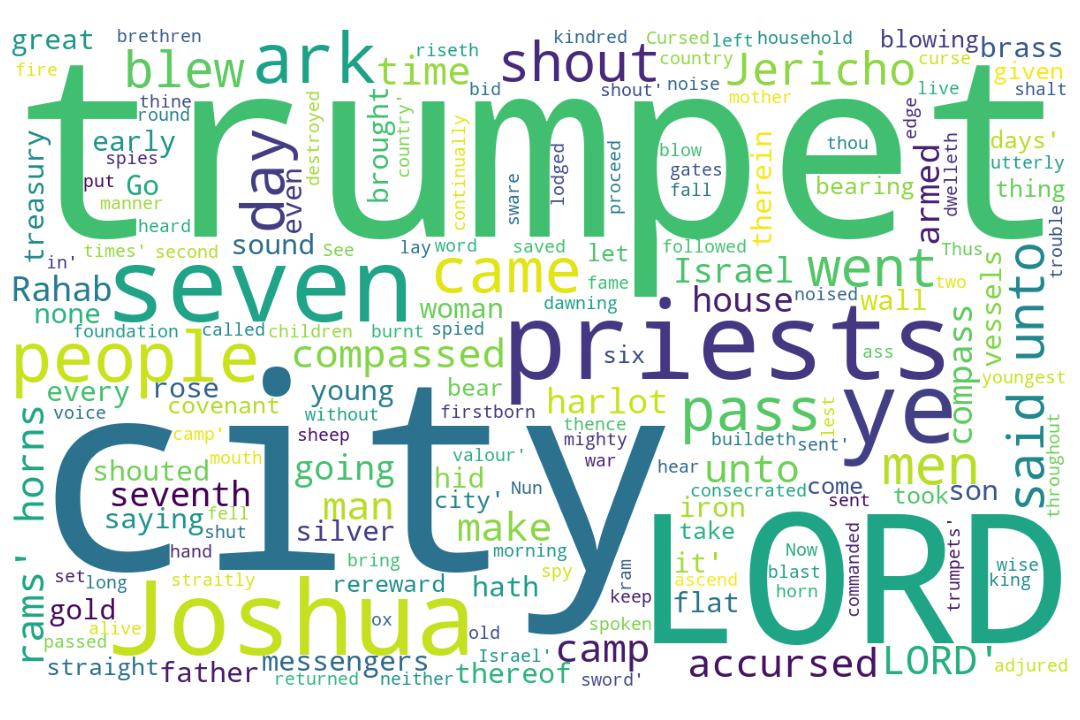
\includegraphics[width=\linewidth]{06OT-Joshua/Joshua6-WordCloud.jpg}
  \caption{Joshua 6 Word Cloud}
  \label{fig:Joshua 6 Word Cloud}
\end{figure}

\marginpar{\scriptsize \centering \fcolorbox{bone}{lime}{\textbf{CONQUERING THE DEVIL'S CITY}}\\ (Joshua 6)

\begin{compactenum}[I.][8]
    \item  The  \textbf{Steady March} \index[scripture]{Joshua!Jsh 06:10}  (Joshua 6:10) 
    \item  The  \textbf{Strange Manners} (of God's People) \index[scripture]{Joshua!Jsh 06:09}  (Jsh 6:9) 
    \item  The  \textbf{Sound of Music}  \index[scripture]{Joshua!Jsh 06:09}  (Jsh 6:9) 
    \item    \textbf{Shouting Men}  \index[scripture]{Joshua!Jsh 06:10}  (Jsh 6:10) 
    \item  A  \textbf{Solemn Message} \index[scripture]{Joshua!Jsh 06:10}  (Jsh 6:10) 
    \item  The  \textbf{Seventh Morning} \index[scripture]{Joshua!Jsh 06:15}  (Jsh 6:15) 
    \item  A  \textbf{Serious Mystery}  \index[scripture]{Joshua!Jsh 06:10}  (Jsh 6:10) 
\end{compactenum}}




\footnote{\href{https://audiobible.com/bible/joshua_6.html}{\textcolor[cmyk]{0.99998,1,0,0}{Joshua 6 Audio}}}\footnote{\textcolor[cmyk]{0.99998,1,0,0}{\hyperlink{TOC}{Return to end of Table of Contents.}}}\textcolor[cmyk]{0.99998,1,0,0}{Now Jericho was straitly shut up because of the children of Israel: none went out, and none came in.}
[2] \textcolor[cmyk]{0.99998,1,0,0}{And the LORD said unto Joshua, See, I have given into thine hand Jericho, and the king thereof, \emph{and} the mighty men of valour.}
[3] \textcolor[cmyk]{0.99998,1,0,0}{And ye shall compass the city, all \emph{ye} men of war, \emph{and} go round about the city once. Thus shalt thou do six days.}
[4] \textcolor[cmyk]{0.99998,1,0,0}{And seven priests shall bear before the ark seven trumpets of rams' horns: and the seventh day ye shall compass the city seven times, and the priests shall blow with the trumpets.}
[5] \textcolor[cmyk]{0.99998,1,0,0}{And it shall come to pass, that when they make a long \emph{blast} with the ram's horn, \emph{and} when ye hear the sound of the trumpet, all the people shall shout with a great shout; and the wall of the city shall fall down flat, and the people shall ascend up every man straight before him.}\\
\\
\P \textcolor[cmyk]{0.99998,1,0,0}{And Joshua the son of Nun called the priests, and said unto them, Take up the ark of the covenant, and let seven priests bear seven trumpets of rams' horns before the ark of the LORD.}
[7] \textcolor[cmyk]{0.99998,1,0,0}{And he said unto the people, Pass on, and compass the city, and let him that is armed pass on before the ark of the LORD.}\\
\\
\P \textcolor[cmyk]{0.99998,1,0,0}{And it came to pass, when Joshua had spoken unto the people, that the seven priests bearing the seven trumpets of rams' horns passed on before the LORD, and blew with the trumpets: and the ark of the covenant of the LORD followed them.}\\
\\
\P  \textcolor[cmyk]{0.99998,1,0,0}{And the armed men went before the priests that blew with the trumpets, and the rereward came after the ark, \emph{the} \emph{priests} going on, and blowing with the trumpets.}
[10] \textcolor[cmyk]{0.99998,1,0,0}{And Joshua had commanded the people, saying, Ye shall not shout, nor make any noise with your voice, neither shall \emph{any} word proceed out of your mouth, until the day I bid you shout; then shall ye shout.} 
[11] \textcolor[cmyk]{0.99998,1,0,0}{So the ark of the LORD compassed the city, going about \emph{it} once: and they came into the camp, and lodged in the camp.}\\
\\
\P \textcolor[cmyk]{0.99998,1,0,0}{And Joshua rose early in the morning, and the priests took up the ark of the LORD.}
[13] \textcolor[cmyk]{0.99998,1,0,0}{And seven priests bearing seven trumpets of rams' horns before the ark of the LORD went on continually, and blew with the trumpets: and the armed men went before them; but the rereward came after the ark of the LORD, \emph{the} \emph{priests} going on, and blowing with the trumpets.}
[14] \textcolor[cmyk]{0.99998,1,0,0}{And the second day they compassed the city once, and returned into the camp: so they did six days.}
[15] \textcolor[cmyk]{0.99998,1,0,0}{And it came to pass on the seventh day, that they rose early about the dawning of the day, and compassed the city after the same manner seven times: only on that day they compassed the city seven times.}
[16] \textcolor[cmyk]{0.99998,1,0,0}{And it came to pass at the seventh time, when the priests blew with the trumpets, Joshua said unto the people, Shout; for the LORD hath given you the city.}\\
\\
\P \textcolor[cmyk]{0.99998,1,0,0}{And the city shall be accursed, \emph{even} it, and all that \emph{are} therein, to the LORD: only Rahab the harlot shall live, she and all that \emph{are} with her in the house, because she hid the messengers that we sent.}
[18] \textcolor[cmyk]{0.99998,1,0,0}{And ye, in any wise keep \emph{yourselves} from the accursed thing, lest ye make \emph{yourselves} accursed, when ye take of the accursed thing, and make the camp of Israel a curse, and trouble it.}
[19] \textcolor[cmyk]{0.99998,1,0,0}{But all the silver, and gold, and vessels of brass and iron, \emph{are} consecrated unto the LORD: they shall come into the treasury of the LORD.}
[20] \textcolor[cmyk]{0.99998,1,0,0}{So the people shouted when \emph{the} \emph{priests} blew with the trumpets: and it came to pass, when the people heard the sound of the trumpet, and the people shouted with a great shout, that the wall fell down flat, so that the people went up into the city, every man straight before him, and they took the city.}
[21] \textcolor[cmyk]{0.99998,1,0,0}{And they utterly destroyed all that \emph{was} in the city, both man and woman, young and old, and ox, and sheep, and ass, with the edge of the sword.}
[22] \textcolor[cmyk]{0.99998,1,0,0}{But Joshua had said unto the two men that had spied out the country, Go into the harlot's house, and bring out thence the woman, and all that she hath, as ye sware unto her.}
[23] \textcolor[cmyk]{0.99998,1,0,0}{And the young men that were spies went in, and brought out Rahab, and her father, and her mother, and her brethren, and all that she had; and they brought out all her kindred, and left them without the camp of Israel.}
[24] \textcolor[cmyk]{0.99998,1,0,0}{And they burnt the city with fire, and all that \emph{was} therein: only the silver, and the gold, and the vessels of brass and of iron, they put into the treasury of the house of the LORD.}
[25] \textcolor[cmyk]{0.99998,1,0,0}{And Joshua saved Rahab the harlot alive, and her father's household, and all that she had; and she dwelleth in Israel \emph{even} unto this day; because she hid the messengers, which Joshua sent to spy out Jericho.}
[26] \textcolor[cmyk]{0.99998,1,0,0}{And Joshua adjured \emph{them} at that time, saying, Cursed \emph{be} the man before the LORD, that riseth up and buildeth this city Jericho: he shall lay the foundation thereof in his firstborn, and in his youngest \emph{son} shall he set up the gates of it.}
[27] \textcolor[cmyk]{0.99998,1,0,0}{So the LORD was with Joshua; and his fame was \emph{noised} throughout all the country.}
\index[NWIV]{19!Joshua!Jos 6:2}\index[AWIP]{Now!Joshua!Jos 6:2}\index[AWIP]{Jericho!Joshua!Jos 6:2}\index[AWIP]{was!Joshua!Jos 6:2}\index[AWIP]{straitly!Joshua!Jos 6:2}\index[AWIP]{shut!Joshua!Jos 6:2}\index[AWIP]{up!Joshua!Jos 6:2}\index[AWIP]{because!Joshua!Jos 6:2}\index[AWIP]{of!Joshua!Jos 6:2}\index[AWIP]{of!Joshua!Jos 6:2 (2)}\index[AWIP]{the!Joshua!Jos 6:2}\index[AWIP]{children!Joshua!Jos 6:2}\index[AWIP]{Israel!Joshua!Jos 6:2}\index[AWIP]{none!Joshua!Jos 6:2}\index[AWIP]{none!Joshua!Jos 6:2 (2)}\index[AWIP]{went!Joshua!Jos 6:2}\index[AWIP]{out!Joshua!Jos 6:2}\index[AWIP]{and!Joshua!Jos 6:2}\index[AWIP]{came!Joshua!Jos 6:2}\index[AWIP]{in!Joshua!Jos 6:2}

\index[NWIV]{24!Joshua!Jos 6:2}\index[AWIP]{And!Joshua!Jos 6:2}\index[AWIP]{the!Joshua!Jos 6:2}\index[AWIP]{the!Joshua!Jos 6:2 (2)}\index[AWIP]{the!Joshua!Jos 6:2 (3)}\index[AWIP]{LORD!Joshua!Jos 6:2}\index[AWIP]{said!Joshua!Jos 6:2}\index[AWIP]{unto!Joshua!Jos 6:2}\index[AWIP]{Joshua!Joshua!Jos 6:2}\index[AWIP]{See!Joshua!Jos 6:2}\index[AWIP]{I!Joshua!Jos 6:2}\index[AWIP]{have!Joshua!Jos 6:2}\index[AWIP]{given!Joshua!Jos 6:2}\index[AWIP]{into!Joshua!Jos 6:2}\index[AWIP]{thine!Joshua!Jos 6:2}\index[AWIP]{hand!Joshua!Jos 6:2}\index[AWIP]{Jericho!Joshua!Jos 6:2}\index[AWIP]{and!Joshua!Jos 6:2}\index[AWIP]{king!Joshua!Jos 6:2}\index[AWIP]{thereof!Joshua!Jos 6:2}\index[AWIP]{\emph{and}!Joshua!Jos 6:2}\index[AWIP]{mighty!Joshua!Jos 6:2}\index[AWIP]{men!Joshua!Jos 6:2}\index[AWIP]{of!Joshua!Jos 6:2}\index[AWIP]{valour!Joshua!Jos 6:2}\index[AWIP]{\emph{and}!Joshua!Jos 6:2}

\index[NWIV]{24!Joshua!Jos 6:3}\index[AWIP]{And!Joshua!Jos 6:3}\index[AWIP]{ye!Joshua!Jos 6:3}\index[AWIP]{shall!Joshua!Jos 6:3}\index[AWIP]{compass!Joshua!Jos 6:3}\index[AWIP]{the!Joshua!Jos 6:3}\index[AWIP]{the!Joshua!Jos 6:3 (2)}\index[AWIP]{city!Joshua!Jos 6:3}\index[AWIP]{city!Joshua!Jos 6:3 (2)}\index[AWIP]{all!Joshua!Jos 6:3}\index[AWIP]{\emph{ye}!Joshua!Jos 6:3}\index[AWIP]{men!Joshua!Jos 6:3}\index[AWIP]{of!Joshua!Jos 6:3}\index[AWIP]{war!Joshua!Jos 6:3}\index[AWIP]{\emph{and}!Joshua!Jos 6:3}\index[AWIP]{go!Joshua!Jos 6:3}\index[AWIP]{round!Joshua!Jos 6:3}\index[AWIP]{about!Joshua!Jos 6:3}\index[AWIP]{once!Joshua!Jos 6:3}\index[AWIP]{Thus!Joshua!Jos 6:3}\index[AWIP]{shalt!Joshua!Jos 6:3}\index[AWIP]{thou!Joshua!Jos 6:3}\index[AWIP]{do!Joshua!Jos 6:3}\index[AWIP]{six!Joshua!Jos 6:3}\index[AWIP]{days!Joshua!Jos 6:3}\index[AWIP]{\emph{ye}!Joshua!Jos 6:3}\index[AWIP]{\emph{and}!Joshua!Jos 6:3}

\index[NWIV]{32!Joshua!Jos 6:4}\index[AWIP]{And!Joshua!Jos 6:4}\index[AWIP]{seven!Joshua!Jos 6:4}\index[AWIP]{seven!Joshua!Jos 6:4 (2)}\index[AWIP]{seven!Joshua!Jos 6:4 (3)}\index[AWIP]{priests!Joshua!Jos 6:4}\index[AWIP]{priests!Joshua!Jos 6:4 (2)}\index[AWIP]{shall!Joshua!Jos 6:4}\index[AWIP]{shall!Joshua!Jos 6:4 (2)}\index[AWIP]{shall!Joshua!Jos 6:4 (3)}\index[AWIP]{bear!Joshua!Jos 6:4}\index[AWIP]{before!Joshua!Jos 6:4}\index[AWIP]{the!Joshua!Jos 6:4}\index[AWIP]{the!Joshua!Jos 6:4 (2)}\index[AWIP]{the!Joshua!Jos 6:4 (3)}\index[AWIP]{the!Joshua!Jos 6:4 (4)}\index[AWIP]{the!Joshua!Jos 6:4 (5)}\index[AWIP]{ark!Joshua!Jos 6:4}\index[AWIP]{trumpets!Joshua!Jos 6:4}\index[AWIP]{trumpets!Joshua!Jos 6:4 (2)}\index[AWIP]{of!Joshua!Jos 6:4}\index[AWIP]{rams'!Joshua!Jos 6:4}\index[AWIP]{horns!Joshua!Jos 6:4}\index[AWIP]{and!Joshua!Jos 6:4}\index[AWIP]{and!Joshua!Jos 6:4 (2)}\index[AWIP]{seventh!Joshua!Jos 6:4}\index[AWIP]{day!Joshua!Jos 6:4}\index[AWIP]{ye!Joshua!Jos 6:4}\index[AWIP]{compass!Joshua!Jos 6:4}\index[AWIP]{city!Joshua!Jos 6:4}\index[AWIP]{times!Joshua!Jos 6:4}\index[AWIP]{blow!Joshua!Jos 6:4}\index[AWIP]{with!Joshua!Jos 6:4}

\index[NWIV]{56!Joshua!Jos 6:5}\index[AWIP]{And!Joshua!Jos 6:5}\index[AWIP]{it!Joshua!Jos 6:5}\index[AWIP]{shall!Joshua!Jos 6:5}\index[AWIP]{shall!Joshua!Jos 6:5 (2)}\index[AWIP]{shall!Joshua!Jos 6:5 (3)}\index[AWIP]{shall!Joshua!Jos 6:5 (4)}\index[AWIP]{come!Joshua!Jos 6:5}\index[AWIP]{to!Joshua!Jos 6:5}\index[AWIP]{pass!Joshua!Jos 6:5}\index[AWIP]{that!Joshua!Jos 6:5}\index[AWIP]{when!Joshua!Jos 6:5}\index[AWIP]{when!Joshua!Jos 6:5 (2)}\index[AWIP]{they!Joshua!Jos 6:5}\index[AWIP]{make!Joshua!Jos 6:5}\index[AWIP]{a!Joshua!Jos 6:5}\index[AWIP]{a!Joshua!Jos 6:5 (2)}\index[AWIP]{long!Joshua!Jos 6:5}\index[AWIP]{\emph{blast}!Joshua!Jos 6:5}\index[AWIP]{with!Joshua!Jos 6:5}\index[AWIP]{with!Joshua!Jos 6:5 (2)}\index[AWIP]{the!Joshua!Jos 6:5}\index[AWIP]{the!Joshua!Jos 6:5 (2)}\index[AWIP]{the!Joshua!Jos 6:5 (3)}\index[AWIP]{the!Joshua!Jos 6:5 (4)}\index[AWIP]{the!Joshua!Jos 6:5 (5)}\index[AWIP]{the!Joshua!Jos 6:5 (6)}\index[AWIP]{the!Joshua!Jos 6:5 (7)}\index[AWIP]{ram's!Joshua!Jos 6:5}\index[AWIP]{horn!Joshua!Jos 6:5}\index[AWIP]{\emph{and}!Joshua!Jos 6:5}\index[AWIP]{ye!Joshua!Jos 6:5}\index[AWIP]{hear!Joshua!Jos 6:5}\index[AWIP]{sound!Joshua!Jos 6:5}\index[AWIP]{of!Joshua!Jos 6:5}\index[AWIP]{of!Joshua!Jos 6:5 (2)}\index[AWIP]{trumpet!Joshua!Jos 6:5}\index[AWIP]{all!Joshua!Jos 6:5}\index[AWIP]{people!Joshua!Jos 6:5}\index[AWIP]{people!Joshua!Jos 6:5 (2)}\index[AWIP]{shout!Joshua!Jos 6:5}\index[AWIP]{shout!Joshua!Jos 6:5 (2)}\index[AWIP]{great!Joshua!Jos 6:5}\index[AWIP]{and!Joshua!Jos 6:5}\index[AWIP]{and!Joshua!Jos 6:5 (2)}\index[AWIP]{wall!Joshua!Jos 6:5}\index[AWIP]{city!Joshua!Jos 6:5}\index[AWIP]{fall!Joshua!Jos 6:5}\index[AWIP]{down!Joshua!Jos 6:5}\index[AWIP]{flat!Joshua!Jos 6:5}\index[AWIP]{ascend!Joshua!Jos 6:5}\index[AWIP]{up!Joshua!Jos 6:5}\index[AWIP]{every!Joshua!Jos 6:5}\index[AWIP]{man!Joshua!Jos 6:5}\index[AWIP]{straight!Joshua!Jos 6:5}\index[AWIP]{before!Joshua!Jos 6:5}\index[AWIP]{him!Joshua!Jos 6:5}\index[AWIP]{\emph{blast}!Joshua!Jos 6:5}\index[AWIP]{\emph{and}!Joshua!Jos 6:5}

\index[NWIV]{36!Joshua!Jos 6:6}\index[AWIP]{And!Joshua!Jos 6:6}\index[AWIP]{Joshua!Joshua!Jos 6:6}\index[AWIP]{the!Joshua!Jos 6:6}\index[AWIP]{the!Joshua!Jos 6:6 (2)}\index[AWIP]{the!Joshua!Jos 6:6 (3)}\index[AWIP]{the!Joshua!Jos 6:6 (4)}\index[AWIP]{the!Joshua!Jos 6:6 (5)}\index[AWIP]{the!Joshua!Jos 6:6 (6)}\index[AWIP]{son!Joshua!Jos 6:6}\index[AWIP]{of!Joshua!Jos 6:6}\index[AWIP]{of!Joshua!Jos 6:6 (2)}\index[AWIP]{of!Joshua!Jos 6:6 (3)}\index[AWIP]{of!Joshua!Jos 6:6 (4)}\index[AWIP]{Nun!Joshua!Jos 6:6}\index[AWIP]{called!Joshua!Jos 6:6}\index[AWIP]{priests!Joshua!Jos 6:6}\index[AWIP]{priests!Joshua!Jos 6:6 (2)}\index[AWIP]{and!Joshua!Jos 6:6}\index[AWIP]{and!Joshua!Jos 6:6 (2)}\index[AWIP]{said!Joshua!Jos 6:6}\index[AWIP]{unto!Joshua!Jos 6:6}\index[AWIP]{them!Joshua!Jos 6:6}\index[AWIP]{Take!Joshua!Jos 6:6}\index[AWIP]{up!Joshua!Jos 6:6}\index[AWIP]{ark!Joshua!Jos 6:6}\index[AWIP]{ark!Joshua!Jos 6:6 (2)}\index[AWIP]{covenant!Joshua!Jos 6:6}\index[AWIP]{let!Joshua!Jos 6:6}\index[AWIP]{seven!Joshua!Jos 6:6}\index[AWIP]{seven!Joshua!Jos 6:6 (2)}\index[AWIP]{bear!Joshua!Jos 6:6}\index[AWIP]{trumpets!Joshua!Jos 6:6}\index[AWIP]{rams'!Joshua!Jos 6:6}\index[AWIP]{horns!Joshua!Jos 6:6}\index[AWIP]{before!Joshua!Jos 6:6}\index[AWIP]{LORD!Joshua!Jos 6:6}

\index[NWIV]{26!Joshua!Jos 6:7}\index[AWIP]{And!Joshua!Jos 6:7}\index[AWIP]{he!Joshua!Jos 6:7}\index[AWIP]{said!Joshua!Jos 6:7}\index[AWIP]{unto!Joshua!Jos 6:7}\index[AWIP]{the!Joshua!Jos 6:7}\index[AWIP]{the!Joshua!Jos 6:7 (2)}\index[AWIP]{the!Joshua!Jos 6:7 (3)}\index[AWIP]{the!Joshua!Jos 6:7 (4)}\index[AWIP]{people!Joshua!Jos 6:7}\index[AWIP]{Pass!Joshua!Jos 6:7}\index[AWIP]{on!Joshua!Jos 6:7}\index[AWIP]{on!Joshua!Jos 6:7 (2)}\index[AWIP]{and!Joshua!Jos 6:7}\index[AWIP]{and!Joshua!Jos 6:7 (2)}\index[AWIP]{compass!Joshua!Jos 6:7}\index[AWIP]{city!Joshua!Jos 6:7}\index[AWIP]{let!Joshua!Jos 6:7}\index[AWIP]{him!Joshua!Jos 6:7}\index[AWIP]{that!Joshua!Jos 6:7}\index[AWIP]{is!Joshua!Jos 6:7}\index[AWIP]{armed!Joshua!Jos 6:7}\index[AWIP]{pass!Joshua!Jos 6:7}\index[AWIP]{before!Joshua!Jos 6:7}\index[AWIP]{ark!Joshua!Jos 6:7}\index[AWIP]{of!Joshua!Jos 6:7}\index[AWIP]{LORD!Joshua!Jos 6:7}

\index[NWIV]{44!Joshua!Jos 6:8}\index[AWIP]{And!Joshua!Jos 6:8}\index[AWIP]{it!Joshua!Jos 6:8}\index[AWIP]{came!Joshua!Jos 6:8}\index[AWIP]{to!Joshua!Jos 6:8}\index[AWIP]{pass!Joshua!Jos 6:8}\index[AWIP]{when!Joshua!Jos 6:8}\index[AWIP]{Joshua!Joshua!Jos 6:8}\index[AWIP]{had!Joshua!Jos 6:8}\index[AWIP]{spoken!Joshua!Jos 6:8}\index[AWIP]{unto!Joshua!Jos 6:8}\index[AWIP]{the!Joshua!Jos 6:8}\index[AWIP]{the!Joshua!Jos 6:8 (2)}\index[AWIP]{the!Joshua!Jos 6:8 (3)}\index[AWIP]{the!Joshua!Jos 6:8 (4)}\index[AWIP]{the!Joshua!Jos 6:8 (5)}\index[AWIP]{the!Joshua!Jos 6:8 (6)}\index[AWIP]{the!Joshua!Jos 6:8 (7)}\index[AWIP]{the!Joshua!Jos 6:8 (8)}\index[AWIP]{people!Joshua!Jos 6:8}\index[AWIP]{that!Joshua!Jos 6:8}\index[AWIP]{seven!Joshua!Jos 6:8}\index[AWIP]{seven!Joshua!Jos 6:8 (2)}\index[AWIP]{priests!Joshua!Jos 6:8}\index[AWIP]{bearing!Joshua!Jos 6:8}\index[AWIP]{trumpets!Joshua!Jos 6:8}\index[AWIP]{trumpets!Joshua!Jos 6:8 (2)}\index[AWIP]{of!Joshua!Jos 6:8}\index[AWIP]{of!Joshua!Jos 6:8 (2)}\index[AWIP]{of!Joshua!Jos 6:8 (3)}\index[AWIP]{rams'!Joshua!Jos 6:8}\index[AWIP]{horns!Joshua!Jos 6:8}\index[AWIP]{passed!Joshua!Jos 6:8}\index[AWIP]{on!Joshua!Jos 6:8}\index[AWIP]{before!Joshua!Jos 6:8}\index[AWIP]{LORD!Joshua!Jos 6:8}\index[AWIP]{LORD!Joshua!Jos 6:8 (2)}\index[AWIP]{and!Joshua!Jos 6:8}\index[AWIP]{and!Joshua!Jos 6:8 (2)}\index[AWIP]{blew!Joshua!Jos 6:8}\index[AWIP]{with!Joshua!Jos 6:8}\index[AWIP]{ark!Joshua!Jos 6:8}\index[AWIP]{covenant!Joshua!Jos 6:8}\index[AWIP]{followed!Joshua!Jos 6:8}\index[AWIP]{them!Joshua!Jos 6:8}

\index[NWIV]{29!Joshua!Jos 6:9}\index[AWIP]{And!Joshua!Jos 6:9}\index[AWIP]{the!Joshua!Jos 6:9}\index[AWIP]{the!Joshua!Jos 6:9 (2)}\index[AWIP]{the!Joshua!Jos 6:9 (3)}\index[AWIP]{the!Joshua!Jos 6:9 (4)}\index[AWIP]{the!Joshua!Jos 6:9 (5)}\index[AWIP]{the!Joshua!Jos 6:9 (6)}\index[AWIP]{armed!Joshua!Jos 6:9}\index[AWIP]{men!Joshua!Jos 6:9}\index[AWIP]{went!Joshua!Jos 6:9}\index[AWIP]{before!Joshua!Jos 6:9}\index[AWIP]{priests!Joshua!Jos 6:9}\index[AWIP]{that!Joshua!Jos 6:9}\index[AWIP]{blew!Joshua!Jos 6:9}\index[AWIP]{with!Joshua!Jos 6:9}\index[AWIP]{with!Joshua!Jos 6:9 (2)}\index[AWIP]{trumpets!Joshua!Jos 6:9}\index[AWIP]{trumpets!Joshua!Jos 6:9 (2)}\index[AWIP]{and!Joshua!Jos 6:9}\index[AWIP]{and!Joshua!Jos 6:9 (2)}\index[AWIP]{rereward!Joshua!Jos 6:9}\index[AWIP]{came!Joshua!Jos 6:9}\index[AWIP]{after!Joshua!Jos 6:9}\index[AWIP]{ark!Joshua!Jos 6:9}\index[AWIP]{\emph{the}!Joshua!Jos 6:9}\index[AWIP]{\emph{priests}!Joshua!Jos 6:9}\index[AWIP]{going!Joshua!Jos 6:9}\index[AWIP]{on!Joshua!Jos 6:9}\index[AWIP]{blowing!Joshua!Jos 6:9}\index[AWIP]{\emph{the}!Joshua!Jos 6:9}\index[AWIP]{\emph{priests}!Joshua!Jos 6:9}

\index[NWIV]{38!Joshua!Jos 6:10}\index[AWIP]{And!Joshua!Jos 6:10}\index[AWIP]{Joshua!Joshua!Jos 6:10}\index[AWIP]{had!Joshua!Jos 6:10}\index[AWIP]{commanded!Joshua!Jos 6:10}\index[AWIP]{the!Joshua!Jos 6:10}\index[AWIP]{the!Joshua!Jos 6:10 (2)}\index[AWIP]{people!Joshua!Jos 6:10}\index[AWIP]{saying!Joshua!Jos 6:10}\index[AWIP]{Ye!Joshua!Jos 6:10}\index[AWIP]{shall!Joshua!Jos 6:10}\index[AWIP]{shall!Joshua!Jos 6:10 (2)}\index[AWIP]{shall!Joshua!Jos 6:10 (3)}\index[AWIP]{not!Joshua!Jos 6:10}\index[AWIP]{shout!Joshua!Jos 6:10}\index[AWIP]{shout!Joshua!Jos 6:10 (2)}\index[AWIP]{shout!Joshua!Jos 6:10 (3)}\index[AWIP]{nor!Joshua!Jos 6:10}\index[AWIP]{make!Joshua!Jos 6:10}\index[AWIP]{any!Joshua!Jos 6:10}\index[AWIP]{noise!Joshua!Jos 6:10}\index[AWIP]{with!Joshua!Jos 6:10}\index[AWIP]{your!Joshua!Jos 6:10}\index[AWIP]{your!Joshua!Jos 6:10 (2)}\index[AWIP]{voice!Joshua!Jos 6:10}\index[AWIP]{neither!Joshua!Jos 6:10}\index[AWIP]{\emph{any}!Joshua!Jos 6:10}\index[AWIP]{word!Joshua!Jos 6:10}\index[AWIP]{proceed!Joshua!Jos 6:10}\index[AWIP]{out!Joshua!Jos 6:10}\index[AWIP]{of!Joshua!Jos 6:10}\index[AWIP]{mouth!Joshua!Jos 6:10}\index[AWIP]{until!Joshua!Jos 6:10}\index[AWIP]{day!Joshua!Jos 6:10}\index[AWIP]{I!Joshua!Jos 6:10}\index[AWIP]{bid!Joshua!Jos 6:10}\index[AWIP]{you!Joshua!Jos 6:10}\index[AWIP]{then!Joshua!Jos 6:10}\index[AWIP]{ye!Joshua!Jos 6:10}\index[AWIP]{\emph{any}!Joshua!Jos 6:10}

\index[NWIV]{24!Joshua!Jos 6:11}\index[AWIP]{So!Joshua!Jos 6:11}\index[AWIP]{the!Joshua!Jos 6:11}\index[AWIP]{the!Joshua!Jos 6:11 (2)}\index[AWIP]{the!Joshua!Jos 6:11 (3)}\index[AWIP]{the!Joshua!Jos 6:11 (4)}\index[AWIP]{the!Joshua!Jos 6:11 (5)}\index[AWIP]{ark!Joshua!Jos 6:11}\index[AWIP]{of!Joshua!Jos 6:11}\index[AWIP]{LORD!Joshua!Jos 6:11}\index[AWIP]{compassed!Joshua!Jos 6:11}\index[AWIP]{city!Joshua!Jos 6:11}\index[AWIP]{going!Joshua!Jos 6:11}\index[AWIP]{about!Joshua!Jos 6:11}\index[AWIP]{\emph{it}!Joshua!Jos 6:11}\index[AWIP]{once!Joshua!Jos 6:11}\index[AWIP]{and!Joshua!Jos 6:11}\index[AWIP]{and!Joshua!Jos 6:11 (2)}\index[AWIP]{they!Joshua!Jos 6:11}\index[AWIP]{came!Joshua!Jos 6:11}\index[AWIP]{into!Joshua!Jos 6:11}\index[AWIP]{camp!Joshua!Jos 6:11}\index[AWIP]{camp!Joshua!Jos 6:11 (2)}\index[AWIP]{lodged!Joshua!Jos 6:11}\index[AWIP]{in!Joshua!Jos 6:11}\index[AWIP]{\emph{it}!Joshua!Jos 6:11}

\index[NWIV]{17!Joshua!Jos 6:12}\index[AWIP]{And!Joshua!Jos 6:12}\index[AWIP]{Joshua!Joshua!Jos 6:12}\index[AWIP]{rose!Joshua!Jos 6:12}\index[AWIP]{early!Joshua!Jos 6:12}\index[AWIP]{in!Joshua!Jos 6:12}\index[AWIP]{the!Joshua!Jos 6:12}\index[AWIP]{the!Joshua!Jos 6:12 (2)}\index[AWIP]{the!Joshua!Jos 6:12 (3)}\index[AWIP]{the!Joshua!Jos 6:12 (4)}\index[AWIP]{morning!Joshua!Jos 6:12}\index[AWIP]{and!Joshua!Jos 6:12}\index[AWIP]{priests!Joshua!Jos 6:12}\index[AWIP]{took!Joshua!Jos 6:12}\index[AWIP]{up!Joshua!Jos 6:12}\index[AWIP]{ark!Joshua!Jos 6:12}\index[AWIP]{of!Joshua!Jos 6:12}\index[AWIP]{LORD!Joshua!Jos 6:12}

\index[NWIV]{49!Joshua!Jos 6:13}\index[AWIP]{And!Joshua!Jos 6:13}\index[AWIP]{seven!Joshua!Jos 6:13}\index[AWIP]{seven!Joshua!Jos 6:13 (2)}\index[AWIP]{priests!Joshua!Jos 6:13}\index[AWIP]{bearing!Joshua!Jos 6:13}\index[AWIP]{trumpets!Joshua!Jos 6:13}\index[AWIP]{trumpets!Joshua!Jos 6:13 (2)}\index[AWIP]{trumpets!Joshua!Jos 6:13 (3)}\index[AWIP]{of!Joshua!Jos 6:13}\index[AWIP]{of!Joshua!Jos 6:13 (2)}\index[AWIP]{of!Joshua!Jos 6:13 (3)}\index[AWIP]{rams'!Joshua!Jos 6:13}\index[AWIP]{horns!Joshua!Jos 6:13}\index[AWIP]{before!Joshua!Jos 6:13}\index[AWIP]{before!Joshua!Jos 6:13 (2)}\index[AWIP]{the!Joshua!Jos 6:13}\index[AWIP]{the!Joshua!Jos 6:13 (2)}\index[AWIP]{the!Joshua!Jos 6:13 (3)}\index[AWIP]{the!Joshua!Jos 6:13 (4)}\index[AWIP]{the!Joshua!Jos 6:13 (5)}\index[AWIP]{the!Joshua!Jos 6:13 (6)}\index[AWIP]{the!Joshua!Jos 6:13 (7)}\index[AWIP]{the!Joshua!Jos 6:13 (8)}\index[AWIP]{ark!Joshua!Jos 6:13}\index[AWIP]{ark!Joshua!Jos 6:13 (2)}\index[AWIP]{LORD!Joshua!Jos 6:13}\index[AWIP]{LORD!Joshua!Jos 6:13 (2)}\index[AWIP]{went!Joshua!Jos 6:13}\index[AWIP]{went!Joshua!Jos 6:13 (2)}\index[AWIP]{on!Joshua!Jos 6:13}\index[AWIP]{on!Joshua!Jos 6:13 (2)}\index[AWIP]{continually!Joshua!Jos 6:13}\index[AWIP]{and!Joshua!Jos 6:13}\index[AWIP]{and!Joshua!Jos 6:13 (2)}\index[AWIP]{and!Joshua!Jos 6:13 (3)}\index[AWIP]{blew!Joshua!Jos 6:13}\index[AWIP]{with!Joshua!Jos 6:13}\index[AWIP]{with!Joshua!Jos 6:13 (2)}\index[AWIP]{armed!Joshua!Jos 6:13}\index[AWIP]{men!Joshua!Jos 6:13}\index[AWIP]{them!Joshua!Jos 6:13}\index[AWIP]{but!Joshua!Jos 6:13}\index[AWIP]{rereward!Joshua!Jos 6:13}\index[AWIP]{came!Joshua!Jos 6:13}\index[AWIP]{after!Joshua!Jos 6:13}\index[AWIP]{\emph{the}!Joshua!Jos 6:13}\index[AWIP]{\emph{priests}!Joshua!Jos 6:13}\index[AWIP]{going!Joshua!Jos 6:13}\index[AWIP]{blowing!Joshua!Jos 6:13}\index[AWIP]{\emph{the}!Joshua!Jos 6:13}\index[AWIP]{\emph{priests}!Joshua!Jos 6:13}

\index[NWIV]{19!Joshua!Jos 6:14}\index[AWIP]{And!Joshua!Jos 6:14}\index[AWIP]{the!Joshua!Jos 6:14}\index[AWIP]{the!Joshua!Jos 6:14 (2)}\index[AWIP]{the!Joshua!Jos 6:14 (3)}\index[AWIP]{second!Joshua!Jos 6:14}\index[AWIP]{day!Joshua!Jos 6:14}\index[AWIP]{they!Joshua!Jos 6:14}\index[AWIP]{they!Joshua!Jos 6:14 (2)}\index[AWIP]{compassed!Joshua!Jos 6:14}\index[AWIP]{city!Joshua!Jos 6:14}\index[AWIP]{once!Joshua!Jos 6:14}\index[AWIP]{and!Joshua!Jos 6:14}\index[AWIP]{returned!Joshua!Jos 6:14}\index[AWIP]{into!Joshua!Jos 6:14}\index[AWIP]{camp!Joshua!Jos 6:14}\index[AWIP]{so!Joshua!Jos 6:14}\index[AWIP]{did!Joshua!Jos 6:14}\index[AWIP]{six!Joshua!Jos 6:14}\index[AWIP]{days!Joshua!Jos 6:14}

\index[NWIV]{39!Joshua!Jos 6:15}\index[AWIP]{And!Joshua!Jos 6:15}\index[AWIP]{it!Joshua!Jos 6:15}\index[AWIP]{came!Joshua!Jos 6:15}\index[AWIP]{to!Joshua!Jos 6:15}\index[AWIP]{pass!Joshua!Jos 6:15}\index[AWIP]{on!Joshua!Jos 6:15}\index[AWIP]{on!Joshua!Jos 6:15 (2)}\index[AWIP]{the!Joshua!Jos 6:15}\index[AWIP]{the!Joshua!Jos 6:15 (2)}\index[AWIP]{the!Joshua!Jos 6:15 (3)}\index[AWIP]{the!Joshua!Jos 6:15 (4)}\index[AWIP]{the!Joshua!Jos 6:15 (5)}\index[AWIP]{the!Joshua!Jos 6:15 (6)}\index[AWIP]{seventh!Joshua!Jos 6:15}\index[AWIP]{day!Joshua!Jos 6:15}\index[AWIP]{day!Joshua!Jos 6:15 (2)}\index[AWIP]{day!Joshua!Jos 6:15 (3)}\index[AWIP]{that!Joshua!Jos 6:15}\index[AWIP]{that!Joshua!Jos 6:15 (2)}\index[AWIP]{they!Joshua!Jos 6:15}\index[AWIP]{they!Joshua!Jos 6:15 (2)}\index[AWIP]{rose!Joshua!Jos 6:15}\index[AWIP]{early!Joshua!Jos 6:15}\index[AWIP]{about!Joshua!Jos 6:15}\index[AWIP]{dawning!Joshua!Jos 6:15}\index[AWIP]{of!Joshua!Jos 6:15}\index[AWIP]{and!Joshua!Jos 6:15}\index[AWIP]{compassed!Joshua!Jos 6:15}\index[AWIP]{compassed!Joshua!Jos 6:15 (2)}\index[AWIP]{city!Joshua!Jos 6:15}\index[AWIP]{city!Joshua!Jos 6:15 (2)}\index[AWIP]{after!Joshua!Jos 6:15}\index[AWIP]{same!Joshua!Jos 6:15}\index[AWIP]{manner!Joshua!Jos 6:15}\index[AWIP]{seven!Joshua!Jos 6:15}\index[AWIP]{seven!Joshua!Jos 6:15 (2)}\index[AWIP]{times!Joshua!Jos 6:15}\index[AWIP]{times!Joshua!Jos 6:15 (2)}\index[AWIP]{only!Joshua!Jos 6:15}

\index[NWIV]{30!Joshua!Jos 6:16}\index[AWIP]{And!Joshua!Jos 6:16}\index[AWIP]{it!Joshua!Jos 6:16}\index[AWIP]{came!Joshua!Jos 6:16}\index[AWIP]{to!Joshua!Jos 6:16}\index[AWIP]{pass!Joshua!Jos 6:16}\index[AWIP]{at!Joshua!Jos 6:16}\index[AWIP]{the!Joshua!Jos 6:16}\index[AWIP]{the!Joshua!Jos 6:16 (2)}\index[AWIP]{the!Joshua!Jos 6:16 (3)}\index[AWIP]{the!Joshua!Jos 6:16 (4)}\index[AWIP]{the!Joshua!Jos 6:16 (5)}\index[AWIP]{the!Joshua!Jos 6:16 (6)}\index[AWIP]{seventh!Joshua!Jos 6:16}\index[AWIP]{time!Joshua!Jos 6:16}\index[AWIP]{when!Joshua!Jos 6:16}\index[AWIP]{priests!Joshua!Jos 6:16}\index[AWIP]{blew!Joshua!Jos 6:16}\index[AWIP]{with!Joshua!Jos 6:16}\index[AWIP]{trumpets!Joshua!Jos 6:16}\index[AWIP]{Joshua!Joshua!Jos 6:16}\index[AWIP]{said!Joshua!Jos 6:16}\index[AWIP]{unto!Joshua!Jos 6:16}\index[AWIP]{people!Joshua!Jos 6:16}\index[AWIP]{Shout!Joshua!Jos 6:16}\index[AWIP]{for!Joshua!Jos 6:16}\index[AWIP]{LORD!Joshua!Jos 6:16}\index[AWIP]{hath!Joshua!Jos 6:16}\index[AWIP]{given!Joshua!Jos 6:16}\index[AWIP]{you!Joshua!Jos 6:16}\index[AWIP]{city!Joshua!Jos 6:16}

\index[NWIV]{40!Joshua!Jos 6:17}\index[AWIP]{And!Joshua!Jos 6:17}\index[AWIP]{the!Joshua!Jos 6:17}\index[AWIP]{the!Joshua!Jos 6:17 (2)}\index[AWIP]{the!Joshua!Jos 6:17 (3)}\index[AWIP]{the!Joshua!Jos 6:17 (4)}\index[AWIP]{the!Joshua!Jos 6:17 (5)}\index[AWIP]{city!Joshua!Jos 6:17}\index[AWIP]{shall!Joshua!Jos 6:17}\index[AWIP]{shall!Joshua!Jos 6:17 (2)}\index[AWIP]{be!Joshua!Jos 6:17}\index[AWIP]{accursed!Joshua!Jos 6:17}\index[AWIP]{\emph{even}!Joshua!Jos 6:17}\index[AWIP]{it!Joshua!Jos 6:17}\index[AWIP]{and!Joshua!Jos 6:17}\index[AWIP]{and!Joshua!Jos 6:17 (2)}\index[AWIP]{all!Joshua!Jos 6:17}\index[AWIP]{all!Joshua!Jos 6:17 (2)}\index[AWIP]{that!Joshua!Jos 6:17}\index[AWIP]{that!Joshua!Jos 6:17 (2)}\index[AWIP]{that!Joshua!Jos 6:17 (3)}\index[AWIP]{\emph{are}!Joshua!Jos 6:17}\index[AWIP]{\emph{are}!Joshua!Jos 6:17 (2)}\index[AWIP]{therein!Joshua!Jos 6:17}\index[AWIP]{to!Joshua!Jos 6:17}\index[AWIP]{LORD!Joshua!Jos 6:17}\index[AWIP]{only!Joshua!Jos 6:17}\index[AWIP]{Rahab!Joshua!Jos 6:17}\index[AWIP]{harlot!Joshua!Jos 6:17}\index[AWIP]{live!Joshua!Jos 6:17}\index[AWIP]{she!Joshua!Jos 6:17}\index[AWIP]{she!Joshua!Jos 6:17 (2)}\index[AWIP]{with!Joshua!Jos 6:17}\index[AWIP]{her!Joshua!Jos 6:17}\index[AWIP]{in!Joshua!Jos 6:17}\index[AWIP]{house!Joshua!Jos 6:17}\index[AWIP]{because!Joshua!Jos 6:17}\index[AWIP]{hid!Joshua!Jos 6:17}\index[AWIP]{messengers!Joshua!Jos 6:17}\index[AWIP]{we!Joshua!Jos 6:17}\index[AWIP]{sent!Joshua!Jos 6:17}\index[AWIP]{\emph{even}!Joshua!Jos 6:17}\index[AWIP]{\emph{are}!Joshua!Jos 6:17}\index[AWIP]{\emph{are}!Joshua!Jos 6:17 (2)}

\index[NWIV]{34!Joshua!Jos 6:18}\index[AWIP]{And!Joshua!Jos 6:18}\index[AWIP]{ye!Joshua!Jos 6:18}\index[AWIP]{ye!Joshua!Jos 6:18 (2)}\index[AWIP]{ye!Joshua!Jos 6:18 (3)}\index[AWIP]{in!Joshua!Jos 6:18}\index[AWIP]{any!Joshua!Jos 6:18}\index[AWIP]{wise!Joshua!Jos 6:18}\index[AWIP]{keep!Joshua!Jos 6:18}\index[AWIP]{\emph{yourselves}!Joshua!Jos 6:18}\index[AWIP]{\emph{yourselves}!Joshua!Jos 6:18 (2)}\index[AWIP]{from!Joshua!Jos 6:18}\index[AWIP]{the!Joshua!Jos 6:18}\index[AWIP]{the!Joshua!Jos 6:18 (2)}\index[AWIP]{the!Joshua!Jos 6:18 (3)}\index[AWIP]{accursed!Joshua!Jos 6:18}\index[AWIP]{accursed!Joshua!Jos 6:18 (2)}\index[AWIP]{accursed!Joshua!Jos 6:18 (3)}\index[AWIP]{thing!Joshua!Jos 6:18}\index[AWIP]{thing!Joshua!Jos 6:18 (2)}\index[AWIP]{lest!Joshua!Jos 6:18}\index[AWIP]{make!Joshua!Jos 6:18}\index[AWIP]{make!Joshua!Jos 6:18 (2)}\index[AWIP]{when!Joshua!Jos 6:18}\index[AWIP]{take!Joshua!Jos 6:18}\index[AWIP]{of!Joshua!Jos 6:18}\index[AWIP]{of!Joshua!Jos 6:18 (2)}\index[AWIP]{and!Joshua!Jos 6:18}\index[AWIP]{and!Joshua!Jos 6:18 (2)}\index[AWIP]{camp!Joshua!Jos 6:18}\index[AWIP]{Israel!Joshua!Jos 6:18}\index[AWIP]{a!Joshua!Jos 6:18}\index[AWIP]{curse!Joshua!Jos 6:18}\index[AWIP]{trouble!Joshua!Jos 6:18}\index[AWIP]{it!Joshua!Jos 6:18}\index[AWIP]{\emph{yourselves}!Joshua!Jos 6:18}\index[AWIP]{\emph{yourselves}!Joshua!Jos 6:18 (2)}

\index[NWIV]{26!Joshua!Jos 6:19}\index[AWIP]{But!Joshua!Jos 6:19}\index[AWIP]{all!Joshua!Jos 6:19}\index[AWIP]{the!Joshua!Jos 6:19}\index[AWIP]{the!Joshua!Jos 6:19 (2)}\index[AWIP]{the!Joshua!Jos 6:19 (3)}\index[AWIP]{the!Joshua!Jos 6:19 (4)}\index[AWIP]{silver!Joshua!Jos 6:19}\index[AWIP]{and!Joshua!Jos 6:19}\index[AWIP]{and!Joshua!Jos 6:19 (2)}\index[AWIP]{and!Joshua!Jos 6:19 (3)}\index[AWIP]{gold!Joshua!Jos 6:19}\index[AWIP]{vessels!Joshua!Jos 6:19}\index[AWIP]{of!Joshua!Jos 6:19}\index[AWIP]{of!Joshua!Jos 6:19 (2)}\index[AWIP]{brass!Joshua!Jos 6:19}\index[AWIP]{iron!Joshua!Jos 6:19}\index[AWIP]{\emph{are}!Joshua!Jos 6:19}\index[AWIP]{consecrated!Joshua!Jos 6:19}\index[AWIP]{unto!Joshua!Jos 6:19}\index[AWIP]{LORD!Joshua!Jos 6:19}\index[AWIP]{LORD!Joshua!Jos 6:19 (2)}\index[AWIP]{they!Joshua!Jos 6:19}\index[AWIP]{shall!Joshua!Jos 6:19}\index[AWIP]{come!Joshua!Jos 6:19}\index[AWIP]{into!Joshua!Jos 6:19}\index[AWIP]{treasury!Joshua!Jos 6:19}\index[AWIP]{\emph{are}!Joshua!Jos 6:19}

\index[NWIV]{58!Joshua!Jos 6:20}\index[AWIP]{So!Joshua!Jos 6:20}\index[AWIP]{the!Joshua!Jos 6:20}\index[AWIP]{the!Joshua!Jos 6:20 (2)}\index[AWIP]{the!Joshua!Jos 6:20 (3)}\index[AWIP]{the!Joshua!Jos 6:20 (4)}\index[AWIP]{the!Joshua!Jos 6:20 (5)}\index[AWIP]{the!Joshua!Jos 6:20 (6)}\index[AWIP]{the!Joshua!Jos 6:20 (7)}\index[AWIP]{the!Joshua!Jos 6:20 (8)}\index[AWIP]{the!Joshua!Jos 6:20 (9)}\index[AWIP]{the!Joshua!Jos 6:20 (10)}\index[AWIP]{people!Joshua!Jos 6:20}\index[AWIP]{people!Joshua!Jos 6:20 (2)}\index[AWIP]{people!Joshua!Jos 6:20 (3)}\index[AWIP]{people!Joshua!Jos 6:20 (4)}\index[AWIP]{shouted!Joshua!Jos 6:20}\index[AWIP]{shouted!Joshua!Jos 6:20 (2)}\index[AWIP]{when!Joshua!Jos 6:20}\index[AWIP]{when!Joshua!Jos 6:20 (2)}\index[AWIP]{\emph{the}!Joshua!Jos 6:20}\index[AWIP]{\emph{priests}!Joshua!Jos 6:20}\index[AWIP]{blew!Joshua!Jos 6:20}\index[AWIP]{with!Joshua!Jos 6:20}\index[AWIP]{with!Joshua!Jos 6:20 (2)}\index[AWIP]{trumpets!Joshua!Jos 6:20}\index[AWIP]{and!Joshua!Jos 6:20}\index[AWIP]{and!Joshua!Jos 6:20 (2)}\index[AWIP]{and!Joshua!Jos 6:20 (3)}\index[AWIP]{it!Joshua!Jos 6:20}\index[AWIP]{came!Joshua!Jos 6:20}\index[AWIP]{to!Joshua!Jos 6:20}\index[AWIP]{pass!Joshua!Jos 6:20}\index[AWIP]{heard!Joshua!Jos 6:20}\index[AWIP]{sound!Joshua!Jos 6:20}\index[AWIP]{of!Joshua!Jos 6:20}\index[AWIP]{trumpet!Joshua!Jos 6:20}\index[AWIP]{a!Joshua!Jos 6:20}\index[AWIP]{great!Joshua!Jos 6:20}\index[AWIP]{shout!Joshua!Jos 6:20}\index[AWIP]{that!Joshua!Jos 6:20}\index[AWIP]{that!Joshua!Jos 6:20 (2)}\index[AWIP]{wall!Joshua!Jos 6:20}\index[AWIP]{fell!Joshua!Jos 6:20}\index[AWIP]{down!Joshua!Jos 6:20}\index[AWIP]{flat!Joshua!Jos 6:20}\index[AWIP]{so!Joshua!Jos 6:20}\index[AWIP]{went!Joshua!Jos 6:20}\index[AWIP]{up!Joshua!Jos 6:20}\index[AWIP]{into!Joshua!Jos 6:20}\index[AWIP]{city!Joshua!Jos 6:20}\index[AWIP]{city!Joshua!Jos 6:20 (2)}\index[AWIP]{every!Joshua!Jos 6:20}\index[AWIP]{man!Joshua!Jos 6:20}\index[AWIP]{straight!Joshua!Jos 6:20}\index[AWIP]{before!Joshua!Jos 6:20}\index[AWIP]{him!Joshua!Jos 6:20}\index[AWIP]{they!Joshua!Jos 6:20}\index[AWIP]{took!Joshua!Jos 6:20}\index[AWIP]{\emph{the}!Joshua!Jos 6:20}\index[AWIP]{\emph{priests}!Joshua!Jos 6:20}

\index[NWIV]{29!Joshua!Jos 6:21}\index[AWIP]{And!Joshua!Jos 6:21}\index[AWIP]{they!Joshua!Jos 6:21}\index[AWIP]{utterly!Joshua!Jos 6:21}\index[AWIP]{destroyed!Joshua!Jos 6:21}\index[AWIP]{all!Joshua!Jos 6:21}\index[AWIP]{that!Joshua!Jos 6:21}\index[AWIP]{\emph{was}!Joshua!Jos 6:21}\index[AWIP]{in!Joshua!Jos 6:21}\index[AWIP]{the!Joshua!Jos 6:21}\index[AWIP]{the!Joshua!Jos 6:21 (2)}\index[AWIP]{the!Joshua!Jos 6:21 (3)}\index[AWIP]{city!Joshua!Jos 6:21}\index[AWIP]{both!Joshua!Jos 6:21}\index[AWIP]{man!Joshua!Jos 6:21}\index[AWIP]{and!Joshua!Jos 6:21}\index[AWIP]{and!Joshua!Jos 6:21 (2)}\index[AWIP]{and!Joshua!Jos 6:21 (3)}\index[AWIP]{and!Joshua!Jos 6:21 (4)}\index[AWIP]{and!Joshua!Jos 6:21 (5)}\index[AWIP]{woman!Joshua!Jos 6:21}\index[AWIP]{young!Joshua!Jos 6:21}\index[AWIP]{old!Joshua!Jos 6:21}\index[AWIP]{ox!Joshua!Jos 6:21}\index[AWIP]{sheep!Joshua!Jos 6:21}\index[AWIP]{ass!Joshua!Jos 6:21}\index[AWIP]{with!Joshua!Jos 6:21}\index[AWIP]{edge!Joshua!Jos 6:21}\index[AWIP]{of!Joshua!Jos 6:21}\index[AWIP]{sword!Joshua!Jos 6:21}\index[AWIP]{\emph{was}!Joshua!Jos 6:21}

\index[NWIV]{35!Joshua!Jos 6:22}\index[AWIP]{But!Joshua!Jos 6:22}\index[AWIP]{Joshua!Joshua!Jos 6:22}\index[AWIP]{had!Joshua!Jos 6:22}\index[AWIP]{had!Joshua!Jos 6:22 (2)}\index[AWIP]{said!Joshua!Jos 6:22}\index[AWIP]{unto!Joshua!Jos 6:22}\index[AWIP]{unto!Joshua!Jos 6:22 (2)}\index[AWIP]{the!Joshua!Jos 6:22}\index[AWIP]{the!Joshua!Jos 6:22 (2)}\index[AWIP]{the!Joshua!Jos 6:22 (3)}\index[AWIP]{the!Joshua!Jos 6:22 (4)}\index[AWIP]{two!Joshua!Jos 6:22}\index[AWIP]{men!Joshua!Jos 6:22}\index[AWIP]{that!Joshua!Jos 6:22}\index[AWIP]{that!Joshua!Jos 6:22 (2)}\index[AWIP]{spied!Joshua!Jos 6:22}\index[AWIP]{out!Joshua!Jos 6:22}\index[AWIP]{out!Joshua!Jos 6:22 (2)}\index[AWIP]{country!Joshua!Jos 6:22}\index[AWIP]{Go!Joshua!Jos 6:22}\index[AWIP]{into!Joshua!Jos 6:22}\index[AWIP]{harlot's!Joshua!Jos 6:22}\index[AWIP]{house!Joshua!Jos 6:22}\index[AWIP]{and!Joshua!Jos 6:22}\index[AWIP]{and!Joshua!Jos 6:22 (2)}\index[AWIP]{bring!Joshua!Jos 6:22}\index[AWIP]{thence!Joshua!Jos 6:22}\index[AWIP]{woman!Joshua!Jos 6:22}\index[AWIP]{all!Joshua!Jos 6:22}\index[AWIP]{she!Joshua!Jos 6:22}\index[AWIP]{hath!Joshua!Jos 6:22}\index[AWIP]{as!Joshua!Jos 6:22}\index[AWIP]{ye!Joshua!Jos 6:22}\index[AWIP]{sware!Joshua!Jos 6:22}\index[AWIP]{her!Joshua!Jos 6:22}

\index[NWIV]{42!Joshua!Jos 6:23}\index[AWIP]{And!Joshua!Jos 6:23}\index[AWIP]{the!Joshua!Jos 6:23}\index[AWIP]{the!Joshua!Jos 6:23 (2)}\index[AWIP]{young!Joshua!Jos 6:23}\index[AWIP]{men!Joshua!Jos 6:23}\index[AWIP]{that!Joshua!Jos 6:23}\index[AWIP]{that!Joshua!Jos 6:23 (2)}\index[AWIP]{were!Joshua!Jos 6:23}\index[AWIP]{spies!Joshua!Jos 6:23}\index[AWIP]{went!Joshua!Jos 6:23}\index[AWIP]{in!Joshua!Jos 6:23}\index[AWIP]{and!Joshua!Jos 6:23}\index[AWIP]{and!Joshua!Jos 6:23 (2)}\index[AWIP]{and!Joshua!Jos 6:23 (3)}\index[AWIP]{and!Joshua!Jos 6:23 (4)}\index[AWIP]{and!Joshua!Jos 6:23 (5)}\index[AWIP]{and!Joshua!Jos 6:23 (6)}\index[AWIP]{and!Joshua!Jos 6:23 (7)}\index[AWIP]{brought!Joshua!Jos 6:23}\index[AWIP]{brought!Joshua!Jos 6:23 (2)}\index[AWIP]{out!Joshua!Jos 6:23}\index[AWIP]{out!Joshua!Jos 6:23 (2)}\index[AWIP]{Rahab!Joshua!Jos 6:23}\index[AWIP]{her!Joshua!Jos 6:23}\index[AWIP]{her!Joshua!Jos 6:23 (2)}\index[AWIP]{her!Joshua!Jos 6:23 (3)}\index[AWIP]{her!Joshua!Jos 6:23 (4)}\index[AWIP]{father!Joshua!Jos 6:23}\index[AWIP]{mother!Joshua!Jos 6:23}\index[AWIP]{brethren!Joshua!Jos 6:23}\index[AWIP]{all!Joshua!Jos 6:23}\index[AWIP]{all!Joshua!Jos 6:23 (2)}\index[AWIP]{she!Joshua!Jos 6:23}\index[AWIP]{had!Joshua!Jos 6:23}\index[AWIP]{they!Joshua!Jos 6:23}\index[AWIP]{kindred!Joshua!Jos 6:23}\index[AWIP]{left!Joshua!Jos 6:23}\index[AWIP]{them!Joshua!Jos 6:23}\index[AWIP]{without!Joshua!Jos 6:23}\index[AWIP]{camp!Joshua!Jos 6:23}\index[AWIP]{of!Joshua!Jos 6:23}\index[AWIP]{Israel!Joshua!Jos 6:23}

\index[NWIV]{37!Joshua!Jos 6:24}\index[AWIP]{And!Joshua!Jos 6:24}\index[AWIP]{they!Joshua!Jos 6:24}\index[AWIP]{they!Joshua!Jos 6:24 (2)}\index[AWIP]{burnt!Joshua!Jos 6:24}\index[AWIP]{the!Joshua!Jos 6:24}\index[AWIP]{the!Joshua!Jos 6:24 (2)}\index[AWIP]{the!Joshua!Jos 6:24 (3)}\index[AWIP]{the!Joshua!Jos 6:24 (4)}\index[AWIP]{the!Joshua!Jos 6:24 (5)}\index[AWIP]{the!Joshua!Jos 6:24 (6)}\index[AWIP]{the!Joshua!Jos 6:24 (7)}\index[AWIP]{city!Joshua!Jos 6:24}\index[AWIP]{with!Joshua!Jos 6:24}\index[AWIP]{fire!Joshua!Jos 6:24}\index[AWIP]{and!Joshua!Jos 6:24}\index[AWIP]{and!Joshua!Jos 6:24 (2)}\index[AWIP]{and!Joshua!Jos 6:24 (3)}\index[AWIP]{and!Joshua!Jos 6:24 (4)}\index[AWIP]{all!Joshua!Jos 6:24}\index[AWIP]{that!Joshua!Jos 6:24}\index[AWIP]{\emph{was}!Joshua!Jos 6:24}\index[AWIP]{therein!Joshua!Jos 6:24}\index[AWIP]{only!Joshua!Jos 6:24}\index[AWIP]{silver!Joshua!Jos 6:24}\index[AWIP]{gold!Joshua!Jos 6:24}\index[AWIP]{vessels!Joshua!Jos 6:24}\index[AWIP]{of!Joshua!Jos 6:24}\index[AWIP]{of!Joshua!Jos 6:24 (2)}\index[AWIP]{of!Joshua!Jos 6:24 (3)}\index[AWIP]{of!Joshua!Jos 6:24 (4)}\index[AWIP]{brass!Joshua!Jos 6:24}\index[AWIP]{iron!Joshua!Jos 6:24}\index[AWIP]{put!Joshua!Jos 6:24}\index[AWIP]{into!Joshua!Jos 6:24}\index[AWIP]{treasury!Joshua!Jos 6:24}\index[AWIP]{house!Joshua!Jos 6:24}\index[AWIP]{LORD!Joshua!Jos 6:24}\index[AWIP]{\emph{was}!Joshua!Jos 6:24}

\index[NWIV]{37!Joshua!Jos 6:25}\index[AWIP]{And!Joshua!Jos 6:25}\index[AWIP]{Joshua!Joshua!Jos 6:25}\index[AWIP]{Joshua!Joshua!Jos 6:25 (2)}\index[AWIP]{saved!Joshua!Jos 6:25}\index[AWIP]{Rahab!Joshua!Jos 6:25}\index[AWIP]{the!Joshua!Jos 6:25}\index[AWIP]{the!Joshua!Jos 6:25 (2)}\index[AWIP]{harlot!Joshua!Jos 6:25}\index[AWIP]{alive!Joshua!Jos 6:25}\index[AWIP]{and!Joshua!Jos 6:25}\index[AWIP]{and!Joshua!Jos 6:25 (2)}\index[AWIP]{and!Joshua!Jos 6:25 (3)}\index[AWIP]{her!Joshua!Jos 6:25}\index[AWIP]{father's!Joshua!Jos 6:25}\index[AWIP]{household!Joshua!Jos 6:25}\index[AWIP]{all!Joshua!Jos 6:25}\index[AWIP]{that!Joshua!Jos 6:25}\index[AWIP]{she!Joshua!Jos 6:25}\index[AWIP]{she!Joshua!Jos 6:25 (2)}\index[AWIP]{she!Joshua!Jos 6:25 (3)}\index[AWIP]{had!Joshua!Jos 6:25}\index[AWIP]{dwelleth!Joshua!Jos 6:25}\index[AWIP]{in!Joshua!Jos 6:25}\index[AWIP]{Israel!Joshua!Jos 6:25}\index[AWIP]{\emph{even}!Joshua!Jos 6:25}\index[AWIP]{unto!Joshua!Jos 6:25}\index[AWIP]{this!Joshua!Jos 6:25}\index[AWIP]{day!Joshua!Jos 6:25}\index[AWIP]{because!Joshua!Jos 6:25}\index[AWIP]{hid!Joshua!Jos 6:25}\index[AWIP]{messengers!Joshua!Jos 6:25}\index[AWIP]{which!Joshua!Jos 6:25}\index[AWIP]{sent!Joshua!Jos 6:25}\index[AWIP]{to!Joshua!Jos 6:25}\index[AWIP]{spy!Joshua!Jos 6:25}\index[AWIP]{out!Joshua!Jos 6:25}\index[AWIP]{Jericho!Joshua!Jos 6:25}\index[AWIP]{\emph{even}!Joshua!Jos 6:25}

\index[NWIV]{45!Joshua!Jos 6:26}\index[AWIP]{And!Joshua!Jos 6:26}\index[AWIP]{Joshua!Joshua!Jos 6:26}\index[AWIP]{adjured!Joshua!Jos 6:26}\index[AWIP]{\emph{them}!Joshua!Jos 6:26}\index[AWIP]{at!Joshua!Jos 6:26}\index[AWIP]{that!Joshua!Jos 6:26}\index[AWIP]{that!Joshua!Jos 6:26 (2)}\index[AWIP]{time!Joshua!Jos 6:26}\index[AWIP]{saying!Joshua!Jos 6:26}\index[AWIP]{Cursed!Joshua!Jos 6:26}\index[AWIP]{\emph{be}!Joshua!Jos 6:26}\index[AWIP]{the!Joshua!Jos 6:26}\index[AWIP]{the!Joshua!Jos 6:26 (2)}\index[AWIP]{the!Joshua!Jos 6:26 (3)}\index[AWIP]{the!Joshua!Jos 6:26 (4)}\index[AWIP]{man!Joshua!Jos 6:26}\index[AWIP]{before!Joshua!Jos 6:26}\index[AWIP]{LORD!Joshua!Jos 6:26}\index[AWIP]{riseth!Joshua!Jos 6:26}\index[AWIP]{up!Joshua!Jos 6:26}\index[AWIP]{up!Joshua!Jos 6:26 (2)}\index[AWIP]{and!Joshua!Jos 6:26}\index[AWIP]{and!Joshua!Jos 6:26 (2)}\index[AWIP]{buildeth!Joshua!Jos 6:26}\index[AWIP]{this!Joshua!Jos 6:26}\index[AWIP]{city!Joshua!Jos 6:26}\index[AWIP]{Jericho!Joshua!Jos 6:26}\index[AWIP]{he!Joshua!Jos 6:26}\index[AWIP]{he!Joshua!Jos 6:26 (2)}\index[AWIP]{shall!Joshua!Jos 6:26}\index[AWIP]{shall!Joshua!Jos 6:26 (2)}\index[AWIP]{lay!Joshua!Jos 6:26}\index[AWIP]{foundation!Joshua!Jos 6:26}\index[AWIP]{thereof!Joshua!Jos 6:26}\index[AWIP]{in!Joshua!Jos 6:26}\index[AWIP]{in!Joshua!Jos 6:26 (2)}\index[AWIP]{his!Joshua!Jos 6:26}\index[AWIP]{his!Joshua!Jos 6:26 (2)}\index[AWIP]{firstborn!Joshua!Jos 6:26}\index[AWIP]{youngest!Joshua!Jos 6:26}\index[AWIP]{\emph{son}!Joshua!Jos 6:26}\index[AWIP]{set!Joshua!Jos 6:26}\index[AWIP]{gates!Joshua!Jos 6:26}\index[AWIP]{of!Joshua!Jos 6:26}\index[AWIP]{it!Joshua!Jos 6:26}\index[AWIP]{\emph{them}!Joshua!Jos 6:26}\index[AWIP]{\emph{be}!Joshua!Jos 6:26}\index[AWIP]{\emph{son}!Joshua!Jos 6:26}

\index[NWIV]{15!Joshua!Jos 6:27}\index[AWIP]{So!Joshua!Jos 6:27}\index[AWIP]{the!Joshua!Jos 6:27}\index[AWIP]{the!Joshua!Jos 6:27 (2)}\index[AWIP]{LORD!Joshua!Jos 6:27}\index[AWIP]{was!Joshua!Jos 6:27}\index[AWIP]{was!Joshua!Jos 6:27 (2)}\index[AWIP]{with!Joshua!Jos 6:27}\index[AWIP]{Joshua!Joshua!Jos 6:27}\index[AWIP]{and!Joshua!Jos 6:27}\index[AWIP]{his!Joshua!Jos 6:27}\index[AWIP]{fame!Joshua!Jos 6:27}\index[AWIP]{\emph{noised}!Joshua!Jos 6:27}\index[AWIP]{throughout!Joshua!Jos 6:27}\index[AWIP]{all!Joshua!Jos 6:27}\index[AWIP]{country!Joshua!Jos 6:27}\index[AWIP]{\emph{noised}!Joshua!Jos 6:27}


\section{Joshua 6 Outlines}

\subsection{My Outlines}

\subsubsection{Conquering the Devil's City}
\index[speaker]{Keith Anthony!Joshua 06 (Conquering the Devil's City)}
\index[series]{Joshua (Keith Anthony)!Joshua 06 (Conquering the Devil's City)}
\index[date]{2018/03/06!Joshua 06 (Conquering the Devil's City) (Keith Anthony)}
\begin{compactenum}[I.]
    \item  The  \textbf{Steady March} \index[scripture]{Joshua!Jsh 06:10}  (Joshua 6:10) 
    \item  The  \textbf{Strange Manners} (of God's People) \index[scripture]{Joshua!Jsh 06:09}  (Jsh 6:9) 
    \item  The  \textbf{Sound of Music}  \index[scripture]{Joshua!Jsh 06:09}  (Jsh 6:9) 
    \item    \textbf{Shouting Men}  \index[scripture]{Joshua!Jsh 06:10}  (Jsh 6:10) 
    \item  A  \textbf{Solemn Message} \index[scripture]{Joshua!Jsh 06:10}  (Jsh 6:10) 
    \item  The  \textbf{Seventh Morning} \index[scripture]{Joshua!Jsh 06:15}  (Jsh 6:15) 
    \item  A  \textbf{Serious Mystery}  \index[scripture]{Joshua!Jsh 06:10}  (Jsh 6:10) 
\end{compactenum}
\subsection{Outlines from Others}


\section{Joshua 6 Comments}


\subsection{Joshua 6 Repeated Phrases}


%%%%%%%%%%
%%%%%%%%%%
\normalsize
 
\begin{center}
\begin{longtable}{|p{3.0in}|p{0.5in}|}
\caption[Joshua 6 Repeated Phrases]{Joshua 6 Repeated Phrases}\label{table:Repeated Phrases Joshua 6} \\
\hline \multicolumn{1}{|c|}{\textbf{Phrase}} & \multicolumn{1}{c|}{\textbf{Frequency}} \\ \hline 
\endfirsthead
 
\multicolumn{2}{c}
{{\bfseries \tablename\ \thetable{} -- continued from previous page}} \\  
\hline \multicolumn{1}{|c|}{\textbf{Phrase}} & \multicolumn{1}{c|}{\textbf{Frequency}} \\ \hline 
\endhead
 
\hline \multicolumn{2}{c}{{ }} \\ \hline
\endfoot 
of the & 19\\ \hline 
the LORD & 16\\ \hline 
the city & 15\\ \hline 
and the & 12\\ \hline 
the ark & 10\\ \hline 
with the & 10\\ \hline 
the people & 10\\ \hline 
of the LORD & 9\\ \hline 
with the trumpets & 8\\ \hline 
the trumpets & 8\\ \hline 
the ark of & 8\\ \hline 
the ark of the & 8\\ \hline 
ark of & 8\\ \hline 
ark of the & 8\\ \hline 
before the & 7\\ \hline 
all that & 7\\ \hline 
the ark of the LORD & 6\\ \hline 
ark of the LORD & 6\\ \hline 
into the & 6\\ \hline 
and all & 6\\ \hline 
and all that & 6\\ \hline 
And the & 5\\ \hline 
said unto & 5\\ \hline 
the priests & 5\\ \hline 
to pass & 5\\ \hline 
And Joshua & 5\\ \hline 
unto the & 5\\ \hline 
blew with & 5\\ \hline 
blew with the & 5\\ \hline 
blew with the trumpets & 5\\ \hline 
the camp & 5\\ \hline 
seven priests & 4\\ \hline 
before the ark & 4\\ \hline 
seven trumpets & 4\\ \hline 
seven trumpets of & 4\\ \hline 
seven trumpets of rams' & 4\\ \hline 
seven trumpets of rams' horns & 4\\ \hline 
trumpets of & 4\\ \hline 
trumpets of rams' & 4\\ \hline 
trumpets of rams' horns & 4\\ \hline 
of rams' & 4\\ \hline 
of rams' horns & 4\\ \hline 
rams' horns & 4\\ \hline 
And it & 4\\ \hline 
it came & 4\\ \hline 
it came to & 4\\ \hline 
it came to pass & 4\\ \hline 
came to & 4\\ \hline 
came to pass & 4\\ \hline 
blew with the trumpets and & 4\\ \hline 
with the trumpets and & 4\\ \hline 
the trumpets and & 4\\ \hline 
trumpets and & 4\\ \hline 
compassed the & 4\\ \hline 
compassed the city & 4\\ \hline 
in the & 4\\ \hline 
and her & 4\\ \hline 
of Israel & 3\\ \hline 
compass the & 3\\ \hline 
compass the city & 3\\ \hline 
the seventh & 3\\ \hline 
seven times & 3\\ \hline 
all the & 3\\ \hline 
up the & 3\\ \hline 
before the ark of & 3\\ \hline 
before the ark of the & 3\\ \hline 
before the ark of the LORD & 3\\ \hline 
said unto the & 3\\ \hline 
unto the people & 3\\ \hline 
on and & 3\\ \hline 
And it came & 3\\ \hline 
And it came to & 3\\ \hline 
And it came to pass & 3\\ \hline 
Joshua had & 3\\ \hline 
that the & 3\\ \hline 
blew with the trumpets and the & 3\\ \hline 
with the trumpets and the & 3\\ \hline 
the trumpets and the & 3\\ \hline 
trumpets and the & 3\\ \hline 
after the & 3\\ \hline 
\emph{the} \emph{priests} & 3\\ \hline 
So the & 3\\ \hline 
and they & 3\\ \hline 
and all that she & 3\\ \hline 
all that she & 3\\ \hline 
that she & 3\\ \hline 
\end{longtable}
\end{center}



%%%%%%%%%%
%%%%%%%%%%



\section{Joshua 6 Statistics}

%%%%%%%%%%%%%%%%%%%%%%%%%%%
%%%%% Word Statistics
%%%%%%%%%%%%%%%%%%%%%%%%%%


\normalsize



\subsection{Chapter Word Statistics}


%%%%%%%%%%
%%%%%%%%%%
 
\begin{center}
\begin{longtable}{l|c|c|c|c}
\caption[Stats for Joshua 6]{Stats for Joshua 6} \label{table:Stats for Joshua 6} \\ 
\hline \multicolumn{1}{|c|}{\textbf{Verse(s)}} & \multicolumn{1}{|c|}{\textbf{Count}} & \multicolumn{1}{|c|}{\textbf{Unique}} & \multicolumn{1}{|c|}{\textbf{Italics}} & \multicolumn{1}{|c|}{\textbf{Uniq Italic}}  \\ \hline 
\endfirsthead
 
\multicolumn{5}{c}
{{\bfseries \tablename\ \thetable{} -- continued from previous page}} \\  
\hline \multicolumn{1}{|c|}{\textbf{Verse(s)}} & \multicolumn{1}{|c|}{\textbf{Count}} & \multicolumn{1}{|c|}{\textbf{Unique}} & \multicolumn{1}{|c|}{\textbf{Italics}} & \multicolumn{1}{|c|}{\textbf{Uniq Italic}}  \\ \hline 
\endhead
 
\hline \multicolumn{5}{|r|}{{Continued if needed}} \\ \hline
\endfoot 
1 & 19 & 17 & 0 & 0\\ \hline
2 & 24 & 22 & 1 & 1\\ \hline
3 & 24 & 22 & 2 & 2\\ \hline
4 & 32 & 21 & 0 & 0\\ \hline
5 & 56 & 40 & 2 & 2\\ \hline
6 & 36 & 24 & 0 & 0\\ \hline
7 & 26 & 21 & 0 & 0\\ \hline
8 & 44 & 31 & 0 & 0\\ \hline
9 & 29 & 21 & 2 & 2\\ \hline
10 & 38 & 32 & 1 & 1\\ \hline
11 & 24 & 18 & 1 & 1\\ \hline
12 & 17 & 14 & 0 & 0\\ \hline
13 & 49 & 29 & 2 & 2\\ \hline
14 & 19 & 16 & 0 & 0\\ \hline
15 & 39 & 25 & 0 & 0\\ \hline
16 & 30 & 25 & 0 & 0\\ \hline
17 & 40 & 29 & 3 & 2\\ \hline
18 & 34 & 23 & 2 & 1\\ \hline
19 & 26 & 19 & 1 & 1\\ \hline
20 & 58 & 39 & 2 & 2\\ \hline
21 & 29 & 23 & 1 & 1\\ \hline
22 & 35 & 27 & 0 & 0\\ \hline
23 & 42 & 28 & 0 & 0\\ \hline
24 & 37 & 24 & 1 & 1\\ \hline
25 & 37 & 31 & 1 & 1\\ \hline
26 & 45 & 35 & 3 & 3\\ \hline
27 & 15 & 13 & 1 & 1\\ \hline
\hline \hline
Total & 904 & 252 & 26 & 15



\end{longtable}
\end{center}

%%%%%%%%%%
%%%%%%%%%%
 
\subsection{Words by Frequency}

\begin{center}
\begin{longtable}{l|r}
\caption[Word Frequencies in Joshua 6]{Word Frequencies in Joshua 6} \label{table:WordsIn-Joshua-6} \\ 
\hline \multicolumn{1}{|c|}{\textbf{Word}} & \multicolumn{1}{c|}{\textbf{Frequency}} \\ \hline 
\endfirsthead
 
\multicolumn{2}{c}
{{\bfseries \tablename\ \thetable{} -- continued from previous page}} \\ 
\hline \multicolumn{1}{|c|}{\textbf{Word}} & \multicolumn{1}{c|}{\textbf{Frequency}} \\ \hline 
\endhead
 
\hline \multicolumn{2}{|r|}{{Continued if needed}} \\ \hline
\endfoot
 
\hline \hline
\endlastfoot
the & 122 \\ \hline
and & 56 \\ \hline
of & 34 \\ \hline
And & 21 \\ \hline
that & 20 \\ \hline
LORD & 16 \\ \hline
shall & 16 \\ \hline
city & 16 \\ \hline
with & 16 \\ \hline
all & 12 \\ \hline
trumpets & 12 \\ \hline
they & 12 \\ \hline
Joshua & 11 \\ \hline
seven & 11 \\ \hline
in & 10 \\ \hline
before & 10 \\ \hline
ark & 10 \\ \hline
people & 10 \\ \hline
unto & 9 \\ \hline
priests & 9 \\ \hline
came & 8 \\ \hline
ye & 8 \\ \hline
it & 8 \\ \hline
on & 8 \\ \hline
up & 7 \\ \hline
out & 7 \\ \hline
into & 7 \\ \hline
day & 7 \\ \hline
to & 7 \\ \hline
when & 7 \\ \hline
she & 7 \\ \hline
her & 7 \\ \hline
went & 6 \\ \hline
men & 6 \\ \hline
pass & 6 \\ \hline
shout & 6 \\ \hline
had & 6 \\ \hline
said & 5 \\ \hline
blew & 5 \\ \hline
camp & 5 \\ \hline
Jericho & 4 \\ \hline
Israel & 4 \\ \hline
rams' & 4 \\ \hline
horns & 4 \\ \hline
make & 4 \\ \hline
a & 4 \\ \hline
man & 4 \\ \hline
them & 4 \\ \hline
compassed & 4 \\ \hline
accursed & 4 \\ \hline
was & 3 \\ \hline
because & 3 \\ \hline
\emph{and} & 3 \\ \hline
compass & 3 \\ \hline
about & 3 \\ \hline
once & 3 \\ \hline
seventh & 3 \\ \hline
times & 3 \\ \hline
him & 3 \\ \hline
he & 3 \\ \hline
armed & 3 \\ \hline
after & 3 \\ \hline
\emph{the} & 3 \\ \hline
\emph{priests} & 3 \\ \hline
going & 3 \\ \hline
So & 3 \\ \hline
only & 3 \\ \hline
\emph{are} & 3 \\ \hline
Rahab & 3 \\ \hline
house & 3 \\ \hline
his & 3 \\ \hline
none & 2 \\ \hline
I & 2 \\ \hline
given & 2 \\ \hline
thereof & 2 \\ \hline
six & 2 \\ \hline
days & 2 \\ \hline
bear & 2 \\ \hline
come & 2 \\ \hline
sound & 2 \\ \hline
trumpet & 2 \\ \hline
great & 2 \\ \hline
wall & 2 \\ \hline
down & 2 \\ \hline
flat & 2 \\ \hline
every & 2 \\ \hline
straight & 2 \\ \hline
covenant & 2 \\ \hline
let & 2 \\ \hline
bearing & 2 \\ \hline
rereward & 2 \\ \hline
blowing & 2 \\ \hline
saying & 2 \\ \hline
any & 2 \\ \hline
your & 2 \\ \hline
you & 2 \\ \hline
rose & 2 \\ \hline
early & 2 \\ \hline
took & 2 \\ \hline
so & 2 \\ \hline
at & 2 \\ \hline
time & 2 \\ \hline
hath & 2 \\ \hline
\emph{even} & 2 \\ \hline
therein & 2 \\ \hline
harlot & 2 \\ \hline
hid & 2 \\ \hline
messengers & 2 \\ \hline
sent & 2 \\ \hline
\emph{yourselves} & 2 \\ \hline
thing & 2 \\ \hline
But & 2 \\ \hline
silver & 2 \\ \hline
gold & 2 \\ \hline
vessels & 2 \\ \hline
brass & 2 \\ \hline
iron & 2 \\ \hline
treasury & 2 \\ \hline
shouted & 2 \\ \hline
\emph{was} & 2 \\ \hline
woman & 2 \\ \hline
young & 2 \\ \hline
country & 2 \\ \hline
brought & 2 \\ \hline
this & 2 \\ \hline
Now & 1 \\ \hline
straitly & 1 \\ \hline
shut & 1 \\ \hline
children & 1 \\ \hline
See & 1 \\ \hline
have & 1 \\ \hline
thine & 1 \\ \hline
hand & 1 \\ \hline
king & 1 \\ \hline
mighty & 1 \\ \hline
valour & 1 \\ \hline
\emph{ye} & 1 \\ \hline
war & 1 \\ \hline
go & 1 \\ \hline
round & 1 \\ \hline
Thus & 1 \\ \hline
shalt & 1 \\ \hline
thou & 1 \\ \hline
do & 1 \\ \hline
blow & 1 \\ \hline
long & 1 \\ \hline
\emph{blast} & 1 \\ \hline
ram's & 1 \\ \hline
horn & 1 \\ \hline
hear & 1 \\ \hline
fall & 1 \\ \hline
ascend & 1 \\ \hline
son & 1 \\ \hline
Nun & 1 \\ \hline
called & 1 \\ \hline
Take & 1 \\ \hline
Pass & 1 \\ \hline
is & 1 \\ \hline
spoken & 1 \\ \hline
passed & 1 \\ \hline
followed & 1 \\ \hline
commanded & 1 \\ \hline
Ye & 1 \\ \hline
not & 1 \\ \hline
nor & 1 \\ \hline
noise & 1 \\ \hline
voice & 1 \\ \hline
neither & 1 \\ \hline
\emph{any} & 1 \\ \hline
word & 1 \\ \hline
proceed & 1 \\ \hline
mouth & 1 \\ \hline
until & 1 \\ \hline
bid & 1 \\ \hline
then & 1 \\ \hline
\emph{it} & 1 \\ \hline
lodged & 1 \\ \hline
morning & 1 \\ \hline
continually & 1 \\ \hline
but & 1 \\ \hline
second & 1 \\ \hline
returned & 1 \\ \hline
did & 1 \\ \hline
dawning & 1 \\ \hline
same & 1 \\ \hline
manner & 1 \\ \hline
Shout & 1 \\ \hline
for & 1 \\ \hline
be & 1 \\ \hline
live & 1 \\ \hline
we & 1 \\ \hline
wise & 1 \\ \hline
keep & 1 \\ \hline
from & 1 \\ \hline
lest & 1 \\ \hline
take & 1 \\ \hline
curse & 1 \\ \hline
trouble & 1 \\ \hline
consecrated & 1 \\ \hline
heard & 1 \\ \hline
fell & 1 \\ \hline
utterly & 1 \\ \hline
destroyed & 1 \\ \hline
both & 1 \\ \hline
old & 1 \\ \hline
ox & 1 \\ \hline
sheep & 1 \\ \hline
ass & 1 \\ \hline
edge & 1 \\ \hline
sword & 1 \\ \hline
two & 1 \\ \hline
spied & 1 \\ \hline
Go & 1 \\ \hline
harlot's & 1 \\ \hline
bring & 1 \\ \hline
thence & 1 \\ \hline
as & 1 \\ \hline
sware & 1 \\ \hline
were & 1 \\ \hline
spies & 1 \\ \hline
father & 1 \\ \hline
mother & 1 \\ \hline
brethren & 1 \\ \hline
kindred & 1 \\ \hline
left & 1 \\ \hline
without & 1 \\ \hline
burnt & 1 \\ \hline
fire & 1 \\ \hline
put & 1 \\ \hline
saved & 1 \\ \hline
alive & 1 \\ \hline
father's & 1 \\ \hline
household & 1 \\ \hline
dwelleth & 1 \\ \hline
which & 1 \\ \hline
spy & 1 \\ \hline
adjured & 1 \\ \hline
\emph{them} & 1 \\ \hline
Cursed & 1 \\ \hline
\emph{be} & 1 \\ \hline
riseth & 1 \\ \hline
buildeth & 1 \\ \hline
lay & 1 \\ \hline
foundation & 1 \\ \hline
firstborn & 1 \\ \hline
youngest & 1 \\ \hline
\emph{son} & 1 \\ \hline
set & 1 \\ \hline
gates & 1 \\ \hline
fame & 1 \\ \hline
\emph{noised} & 1 \\ \hline
throughout & 1 \\ \hline
\end{longtable}
\end{center}



\normalsize



\subsection{Words Alphabetically}

\begin{center}
\begin{longtable}{l|r}
\caption[Word Alphabetically in Joshua 6]{Word Alphabetically in Joshua 6} \label{table:WordsIn-Joshua-6} \\ 
\hline \multicolumn{1}{|c|}{\textbf{Word}} & \multicolumn{1}{c|}{\textbf{Frequency}} \\ \hline 
\endfirsthead
 
\multicolumn{2}{c}
{{\bfseries \tablename\ \thetable{} -- continued from previous page}} \\ 
\hline \multicolumn{1}{|c|}{\textbf{Word}} & \multicolumn{1}{c|}{\textbf{Frequency}} \\ \hline 
\endhead
 
\hline \multicolumn{2}{|r|}{{Continued if needed}} \\ \hline
\endfoot
 
\hline \hline
\endlastfoot
And & 21 \\ \hline
But & 2 \\ \hline
Cursed & 1 \\ \hline
Go & 1 \\ \hline
I & 2 \\ \hline
Israel & 4 \\ \hline
Jericho & 4 \\ \hline
Joshua & 11 \\ \hline
LORD & 16 \\ \hline
Now & 1 \\ \hline
Nun & 1 \\ \hline
Pass & 1 \\ \hline
Rahab & 3 \\ \hline
See & 1 \\ \hline
Shout & 1 \\ \hline
So & 3 \\ \hline
Take & 1 \\ \hline
Thus & 1 \\ \hline
Ye & 1 \\ \hline
\emph{and} & 3 \\ \hline
\emph{any} & 1 \\ \hline
\emph{are} & 3 \\ \hline
\emph{be} & 1 \\ \hline
\emph{blast} & 1 \\ \hline
\emph{even} & 2 \\ \hline
\emph{it} & 1 \\ \hline
\emph{noised} & 1 \\ \hline
\emph{priests} & 3 \\ \hline
\emph{son} & 1 \\ \hline
\emph{them} & 1 \\ \hline
\emph{the} & 3 \\ \hline
\emph{was} & 2 \\ \hline
\emph{ye} & 1 \\ \hline
\emph{yourselves} & 2 \\ \hline
a & 4 \\ \hline
about & 3 \\ \hline
accursed & 4 \\ \hline
adjured & 1 \\ \hline
after & 3 \\ \hline
alive & 1 \\ \hline
all & 12 \\ \hline
and & 56 \\ \hline
any & 2 \\ \hline
ark & 10 \\ \hline
armed & 3 \\ \hline
as & 1 \\ \hline
ascend & 1 \\ \hline
ass & 1 \\ \hline
at & 2 \\ \hline
be & 1 \\ \hline
bear & 2 \\ \hline
bearing & 2 \\ \hline
because & 3 \\ \hline
before & 10 \\ \hline
bid & 1 \\ \hline
blew & 5 \\ \hline
blow & 1 \\ \hline
blowing & 2 \\ \hline
both & 1 \\ \hline
brass & 2 \\ \hline
brethren & 1 \\ \hline
bring & 1 \\ \hline
brought & 2 \\ \hline
buildeth & 1 \\ \hline
burnt & 1 \\ \hline
but & 1 \\ \hline
called & 1 \\ \hline
came & 8 \\ \hline
camp & 5 \\ \hline
children & 1 \\ \hline
city & 16 \\ \hline
come & 2 \\ \hline
commanded & 1 \\ \hline
compass & 3 \\ \hline
compassed & 4 \\ \hline
consecrated & 1 \\ \hline
continually & 1 \\ \hline
country & 2 \\ \hline
covenant & 2 \\ \hline
curse & 1 \\ \hline
dawning & 1 \\ \hline
day & 7 \\ \hline
days & 2 \\ \hline
destroyed & 1 \\ \hline
did & 1 \\ \hline
do & 1 \\ \hline
down & 2 \\ \hline
dwelleth & 1 \\ \hline
early & 2 \\ \hline
edge & 1 \\ \hline
every & 2 \\ \hline
fall & 1 \\ \hline
fame & 1 \\ \hline
father & 1 \\ \hline
father's & 1 \\ \hline
fell & 1 \\ \hline
fire & 1 \\ \hline
firstborn & 1 \\ \hline
flat & 2 \\ \hline
followed & 1 \\ \hline
for & 1 \\ \hline
foundation & 1 \\ \hline
from & 1 \\ \hline
gates & 1 \\ \hline
given & 2 \\ \hline
go & 1 \\ \hline
going & 3 \\ \hline
gold & 2 \\ \hline
great & 2 \\ \hline
had & 6 \\ \hline
hand & 1 \\ \hline
harlot & 2 \\ \hline
harlot's & 1 \\ \hline
hath & 2 \\ \hline
have & 1 \\ \hline
he & 3 \\ \hline
hear & 1 \\ \hline
heard & 1 \\ \hline
her & 7 \\ \hline
hid & 2 \\ \hline
him & 3 \\ \hline
his & 3 \\ \hline
horn & 1 \\ \hline
horns & 4 \\ \hline
house & 3 \\ \hline
household & 1 \\ \hline
in & 10 \\ \hline
into & 7 \\ \hline
iron & 2 \\ \hline
is & 1 \\ \hline
it & 8 \\ \hline
keep & 1 \\ \hline
kindred & 1 \\ \hline
king & 1 \\ \hline
lay & 1 \\ \hline
left & 1 \\ \hline
lest & 1 \\ \hline
let & 2 \\ \hline
live & 1 \\ \hline
lodged & 1 \\ \hline
long & 1 \\ \hline
make & 4 \\ \hline
man & 4 \\ \hline
manner & 1 \\ \hline
men & 6 \\ \hline
messengers & 2 \\ \hline
mighty & 1 \\ \hline
morning & 1 \\ \hline
mother & 1 \\ \hline
mouth & 1 \\ \hline
neither & 1 \\ \hline
noise & 1 \\ \hline
none & 2 \\ \hline
nor & 1 \\ \hline
not & 1 \\ \hline
of & 34 \\ \hline
old & 1 \\ \hline
on & 8 \\ \hline
once & 3 \\ \hline
only & 3 \\ \hline
out & 7 \\ \hline
ox & 1 \\ \hline
pass & 6 \\ \hline
passed & 1 \\ \hline
people & 10 \\ \hline
priests & 9 \\ \hline
proceed & 1 \\ \hline
put & 1 \\ \hline
ram's & 1 \\ \hline
rams' & 4 \\ \hline
rereward & 2 \\ \hline
returned & 1 \\ \hline
riseth & 1 \\ \hline
rose & 2 \\ \hline
round & 1 \\ \hline
said & 5 \\ \hline
same & 1 \\ \hline
saved & 1 \\ \hline
saying & 2 \\ \hline
second & 1 \\ \hline
sent & 2 \\ \hline
set & 1 \\ \hline
seven & 11 \\ \hline
seventh & 3 \\ \hline
shall & 16 \\ \hline
shalt & 1 \\ \hline
she & 7 \\ \hline
sheep & 1 \\ \hline
shout & 6 \\ \hline
shouted & 2 \\ \hline
shut & 1 \\ \hline
silver & 2 \\ \hline
six & 2 \\ \hline
so & 2 \\ \hline
son & 1 \\ \hline
sound & 2 \\ \hline
spied & 1 \\ \hline
spies & 1 \\ \hline
spoken & 1 \\ \hline
spy & 1 \\ \hline
straight & 2 \\ \hline
straitly & 1 \\ \hline
sware & 1 \\ \hline
sword & 1 \\ \hline
take & 1 \\ \hline
that & 20 \\ \hline
the & 122 \\ \hline
them & 4 \\ \hline
then & 1 \\ \hline
thence & 1 \\ \hline
therein & 2 \\ \hline
thereof & 2 \\ \hline
they & 12 \\ \hline
thine & 1 \\ \hline
thing & 2 \\ \hline
this & 2 \\ \hline
thou & 1 \\ \hline
throughout & 1 \\ \hline
time & 2 \\ \hline
times & 3 \\ \hline
to & 7 \\ \hline
took & 2 \\ \hline
treasury & 2 \\ \hline
trouble & 1 \\ \hline
trumpet & 2 \\ \hline
trumpets & 12 \\ \hline
two & 1 \\ \hline
until & 1 \\ \hline
unto & 9 \\ \hline
up & 7 \\ \hline
utterly & 1 \\ \hline
valour & 1 \\ \hline
vessels & 2 \\ \hline
voice & 1 \\ \hline
wall & 2 \\ \hline
war & 1 \\ \hline
was & 3 \\ \hline
we & 1 \\ \hline
went & 6 \\ \hline
were & 1 \\ \hline
when & 7 \\ \hline
which & 1 \\ \hline
wise & 1 \\ \hline
with & 16 \\ \hline
without & 1 \\ \hline
woman & 2 \\ \hline
word & 1 \\ \hline
ye & 8 \\ \hline
you & 2 \\ \hline
young & 2 \\ \hline
youngest & 1 \\ \hline
your & 2 \\ \hline
\end{longtable}
\end{center}



\normalsize



\subsection{Word Lengths in Chapter}
\normalsize
\begin{longtable}{l|p{3.75in}}
\caption[Words by Length in Joshua 6]{Words by Length in Joshua 6} \label{table:WordsIn-Joshua-6} \\ 
\hline \multicolumn{1}{|c|}{\textbf{Length}} & \multicolumn{1}{c|}{\textbf{Words}} \\ \hline 
\endfirsthead
 
\multicolumn{2}{c}
{{\bfseries \tablename\ \thetable{} -- continued from previous page}} \\ 
\hline \multicolumn{1}{|c|}{\textbf{Length}} & \multicolumn{1}{c|}{\textbf{Words}} \\ \hline 
\endhead
 
\hline \multicolumn{2}{|r|}{{Continued if needed}} \\ \hline
\endfoot
 
\hline \hline
\endlastfoot
1 & I, a \\ \hline
2 & up, of, in, ye, \emph{ye}, go, do, it, to, he, on, is, Ye, So, \emph{it}, so, at, be, we, ox, Go, as, \emph{be} \\ \hline
3 & Now, was, the, out, and, And, See, \emph{and}, men, all, war, six, ark, day, man, him, son, Nun, let, had, \emph{the}, not, nor, any, \emph{any}, bid, you, but, did, for, \emph{are}, she, her, hid, But, \emph{was}, old, ass, two, put, spy, lay, his, \emph{son}, set \\ \hline
4 & shut, none, went, came, LORD, said, unto, have, into, hand, king, city, once, Thus, thou, days, bear, blow, with, come, pass, that, when, they, make, long, horn, hear, wall, fall, down, flat, them, Take, Pass, blew, your, word, then, camp, rose, took, same, only, time, hath, \emph{even}, live, sent, wise, keep, from, lest, take, gold, iron, fell, both, edge, were, left, fire, this, \emph{them}, fame \\ \hline
5 & given, thine, shall, round, about, shalt, seven, rams', horns, times, \emph{blast}, ram's, sound, shout, great, every, armed, after, going, noise, voice, mouth, until, early, Shout, Rahab, house, thing, curse, brass, heard, woman, young, sheep, sword, spied, bring, sware, spies, burnt, saved, alive, which, gates \\ \hline
6 & Israel, Joshua, mighty, valour, before, people, ascend, called, spoken, passed, saying, lodged, second, manner, harlot, silver, thence, father, mother, Cursed, riseth, \emph{noised} \\ \hline
7 & Jericho, because, thereof, compass, priests, seventh, trumpet, bearing, \emph{priests}, blowing, neither, proceed, morning, dawning, therein, trouble, vessels, shouted, utterly, country, brought, kindred, without, adjured \\ \hline
8 & straitly, children, trumpets, straight, covenant, followed, rereward, returned, accursed, treasury, harlot's, brethren, father's, dwelleth, buildeth, youngest \\ \hline
9 & commanded, compassed, destroyed, household, firstborn \\ \hline
10 & messengers, \emph{yourselves}, foundation, throughout \\ \hline
11 & continually, consecrated \\ \hline
\end{longtable}






%%%%%%%%%%
%%%%%%%%%%

\chapter{Psalm 66}

\begin{figure}
  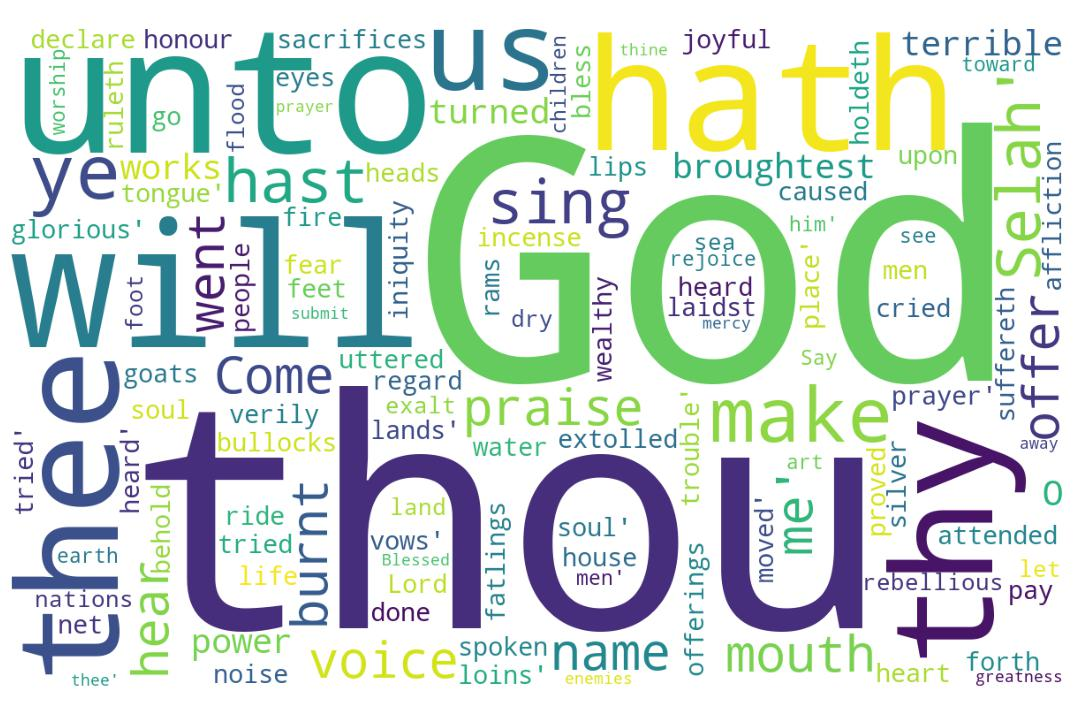
\includegraphics[width=\linewidth]{19OT-Psalms/Psalm66-WordCloud.jpg}
  \caption{Psalm 66 Word Cloud}
  \label{fig:Psalm 66 word Cloud}
\end{figure}

\marginpar{\scriptsize \centering \fcolorbox{bone}{lime}{\textbf{BE THANKFUL}}\\ (Psalm 66:1-20) \begin{compactenum}[I.][8]
    \item The \textbf{Prime Directive} (Futility) \index[scripture]{Psalms!Psa 066:01} Psa 66:1
    \item The \textbf{Path that was Dry}  \index[scripture]{Psalms!Psa 066:06} Psa 66:6
    \item \textbf{Perpetual Dominion} \index[scripture]{Psalms!Psa 066:07} Psa 66:7
    \item A \textbf{Profitable Decision} \index[scripture]{Psalms!Psa 066:13} Psa 66:13
    \item A \textbf{Positive Declaration} \index[scripture]{Psalms!Psa 066:16} Psa 66:16
    \item A \textbf{Pure Difference} \index[scripture]{Psalms!Psa 066:18} Psa 66:18
\end{compactenum}}

\footnote{\textcolor[rgb]{0.00,0.25,0.00}{\hyperlink{TOC}{Return to end of Table of Contents.}}}\footnote{\href{https://audiobible.com/bible/psalms_66.html}{\textcolor[cmyk]{0.99998,1,0,0}{Psalm 66 Audio}}}\textcolor[cmyk]{0.99998,1,0,0}{To the chief Musician, A Song \emph{or} Psalm.}\\
\\
\P \textcolor[cmyk]{0.99998,1,0,0}{Make a \fcolorbox{bone}{lime}{joyful noise} unto God, all ye lands:} %\footnote{Most of this Psalm deals with the Second Advent. Verses 3, 7, 12--13, and 15 are all Millennial references, and the Jews’ “tribulations” will be found in verses 10---12, and 14. You may expect the usual. The “godly” commentators will either miss the doctrinal import of the verses completely or, like Jamieson and Kroll, they will “hint” that perhaps the verses have a future application to some victory, by someone over someone, that will eventually take place sometime. Muddled incoherence is one the characteristics of the exegesis by apostate Fundamentalists when they hit a verse in the King James English that they either don’t like or cannot understand. (This is amply demonstrated in our Commentary on the Psalms). “All ye lands” (vs. 1). This means the heathen (the Gentiles), as in Deuteronomy 32:43 and Romans 11:12--13. Of course, we can make spiritual application. A “joyful noise” by a congregation is better than a smooth, slick, well-executed choir number by professional TV watchers (see Ps. 33:3). The Gregorian chants and Latin “masses” and “requiems” are exactly what is NOT meant by the verse. The song is aimed at God, not the listener (“unto God”). His honor is to be sung, and His praise is to be made “glorious.” The text of the song is given, for the wording follows “Say unto God.” The crucial “Selah” pops up again (for the fortieth time) to warn the “qualified authorities” and “recognized scholars” they are in trouble if they don’t believe THE BOOK. \\
%\\
%Good old Kroll (representing Liberty University) slides by as smooth and slick as a garter snake in a pool of oil. He puts verse 1 in the present tense to get rid of Deuteronomy 32:43 and Isaiah 14:7, and then expostulates on verse 4 saying, “His enemies shall be brought to forced submission under His feet.” Who are His enemies? Zero. When are they brought into submission? Zero. Is “under His feet” literal (Isa. 63:1--6) or figurative? Zero. This is the Swindoll-MacArthur-Bob Jones IV “life-style.” Get through without being detected. Don’t let ’em know what you believe. It is too costly. Dummelow and Kyle Yates are much more honest: one throws the verse out, and the other one says, “The Psalmist takes the whole world in at one sweep, as he sounds the call and gives the proper words for the expression of true praise,” which, of course, means absolutely NOTHING. If we accepted Kroll’s sterile and ambiguous comments, think what we would be missing, even devotionally. 1. Where are the joyful songs about the names of Mohammed, Buddha, Mao Tsetung, Brahma, the popes, and Moses? It says “sing to thy name” (vs. 4). Singing is a manifestation of JOY (“make a joyful noise”). Where are ten songs praising Buddha? Where are fifty praising Mohammed? I have four different hymn books in my house, and between them they present seven hundred different songs about one man. My two German hymnals have fifty more songs which are not in the English hymnals. How does the founder of one religion rate seven hundred fifty songs, while all the others combined can’t produce two hundred songs? Someone’s religion fails to produce JOY. 2. “Thy name” is recommended, so out come Jesus Saves, What a Friend We Have in Jesus, My Jesus I Love Thee, Fairest Lord Jesus, Jesus Is The Sweetest Name I Know, No One Ever Cared for Me Like Jesus, The Light of the World Is Jesus, Jesus What a Friend of Sinners, Jesus the Very Thought of Thee, etc.\cite{Ruckman1992Psalms} }
[2] \textcolor[cmyk]{0.99998,1,0,0}{Sing forth the honour of his name: make his praise glorious.}
[3] \textcolor[cmyk]{0.99998,1,0,0}{Say unto God, How terrible \emph{art} \emph{thou} \emph{in} thy works! through the greatness of thy power shall thine enemies submit themselves unto thee.} %\footnote{The song of verses 2 and 3 has at times come to your ears; for, as Talmage says: “I think sometimes it must break out over the battlements of heaven where the hosts are engaged in perpetual praise.” It is a song about “JESUS”—the One who made our solar system, the One who gave us life, the One who protected us as children, the One who brought us through many dangers, toils, and snares, the One who redeemed us and granted us the New Birth, and the One who will meet us at the end of the race (Hebrews 12:1--3), and grant us an eternity of enjoying the presence of God.\cite{Ruckman1992Psalms} }
[4] \textcolor[cmyk]{0.99998,1,0,0}{All the earth shall worship thee, and shall sing unto thee; they shall sing \emph{to} thy name. Selah.}
[5] \textcolor[cmyk]{0.99998,1,0,0}{Come and see the works of God: \emph{he} \emph{is} terrible \emph{in} \emph{his} doing toward the children of men.} %\footnote{The word “terrible,” verse 5, is used in the sense of “awesome” (as in verse 3), not as the word “rotten” is used today. Observe the same thing in Revelation 17:6 where the word “admiration” is used in the sense of “awesome,” not in the sense of something to be worshipped or bragged about. \cite{Ruckman1992Psalms} }
[6] \textcolor[cmyk]{0.99998,1,0,0}{He turned the sea into \fcolorbox{bone}{lime}{dry \emph{land}}: they went through the flood on foot: there did we rejoice in him.} %\footnote{Verse 6, historically, is the Red Sea crossing. All of the commentators (100 percent) missed the advanced revelation given 380 years ago, that it will happen again in Revelation 12:15, which matches the “flood” prophesied in Daniel 9:26. This flood is connected with the Jordan River (Job 40:23). Note that the first song --  and the context of verse 6 is singing (vss. 1--2) -- was sung at the Red Sea crossing (Exod. 15:1). The “song of Moses” is sung by the Tribulation Saints (Rev. 15:3): “there did we rejoice in him” (vs. 6). The “water” of verse 12 that Israel will pass through is NOT the Red Sea that they had already passed through. Psalm 18:15 corrects the foolishness of the commentators (Yates, Kroll, Motyer, et al.). All of them kill the prophecy by throwing it backwards 500---600 years. Typical; absolutely typical. \cite{Ruckman1992Psalms} }
[7] \textcolor[cmyk]{0.99998,1,0,0}{He ruleth by his power \fcolorbox{bone}{lime}{for ever}; his eyes behold the nations: let not the rebellious exalt themselves. Selah.}
[8] \textcolor[cmyk]{0.99998,1,0,0}{O bless our God, ye people, and make the voice of his praise to be heard:}
[9] \textcolor[cmyk]{0.99998,1,0,0}{Which holdeth our soul in life, and suffereth not our feet to be moved.}
[10] \textcolor[cmyk]{0.99998,1,0,0}{For thou, O God, hast proved us: thou hast tried us, as silver is tried.}\footnote{\textbf{Psalm 12:6} - The words of the LORD are pure words: as silver tried in a furnace of earth, purified seven times.}\footnote{\textbf{1 Peter 1:7} -That the trial of your faith, being much more precious than of gold that perisheth, though it be tried with fire, might be found unto praise and honour and glory at the appearing of Jesus Christ:}
[11] \textcolor[cmyk]{0.99998,1,0,0}{Thou broughtest us into the net; thou laidst affliction upon our loins.}
[12] \textcolor[cmyk]{0.99998,1,0,0}{Thou hast caused men to ride over our heads; we went through fire and through water: but thou broughtest us out into a wealthy \emph{place}.}
[13] \textcolor[cmyk]{0.99998,1,0,0}{I will go into thy house with burnt offerings: I will \fcolorbox{bone}{lime}{pay} thee my vows,}
[14] \textcolor[cmyk]{0.99998,1,0,0}{Which my lips have uttered, and my mouth hath spoken, when I was in trouble.}
[15] \textcolor[cmyk]{0.99998,1,0,0}{I will offer unto thee burnt sacrifices of fatlings, with the incense of rams; I will offer bullocks with goats. Selah.}
[16] \textcolor[cmyk]{0.99998,1,0,0}{Come \emph{and} hear, all ye that fear God, and \fcolorbox{bone}{lime}{I will declare} what he hath done for my soul.}
[17] \textcolor[cmyk]{0.99998,1,0,0}{I cried unto him with my mouth, and he was extolled with my tongue.}
[18] \textcolor[cmyk]{0.99998,1,0,0}{If I \fcolorbox{bone}{lime}{regard iniquity} in my heart, the Lord will not hear \emph{me}:}
[19] \textcolor[cmyk]{0.99998,1,0,0}{\emph{But} verily God hath heard \emph{me}; he hath attended to the voice of my prayer.}
[20] \textcolor[cmyk]{0.99998,1,0,0}{Blessed \emph{be} God, which hath not turned away my prayer, nor his mercy from me.}





\index[NWIV]{9!Psalms!Psa 66:1}\index[AWIP]{Make!Psalms!Psa 66:1}\index[AWIP]{a!Psalms!Psa 66:1}\index[AWIP]{joyful!Psalms!Psa 66:1}\index[AWIP]{noise!Psalms!Psa 66:1}\index[AWIP]{unto!Psalms!Psa 66:1}\index[AWIP]{God!Psalms!Psa 66:1}\index[AWIP]{all!Psalms!Psa 66:1}\index[AWIP]{ye!Psalms!Psa 66:1}\index[AWIP]{lands!Psalms!Psa 66:1}

\index[NWIV]{11!Psalms!Psa 66:2}\index[AWIP]{Sing!Psalms!Psa 66:2}\index[AWIP]{forth!Psalms!Psa 66:2}\index[AWIP]{the!Psalms!Psa 66:2}\index[AWIP]{honour!Psalms!Psa 66:2}\index[AWIP]{of!Psalms!Psa 66:2}\index[AWIP]{his!Psalms!Psa 66:2}\index[AWIP]{his!Psalms!Psa 66:2 (2)}\index[AWIP]{name!Psalms!Psa 66:2}\index[AWIP]{make!Psalms!Psa 66:2}\index[AWIP]{praise!Psalms!Psa 66:2}\index[AWIP]{glorious!Psalms!Psa 66:2}

\index[NWIV]{23!Psalms!Psa 66:3}\index[AWIP]{Say!Psalms!Psa 66:3}\index[AWIP]{unto!Psalms!Psa 66:3}\index[AWIP]{unto!Psalms!Psa 66:3 (2)}\index[AWIP]{God!Psalms!Psa 66:3}\index[AWIP]{How!Psalms!Psa 66:3}\index[AWIP]{terrible!Psalms!Psa 66:3}\index[AWIP]{\emph{art}!Psalms!Psa 66:3}\index[AWIP]{\emph{thou}!Psalms!Psa 66:3}\index[AWIP]{\emph{in}!Psalms!Psa 66:3}\index[AWIP]{thy!Psalms!Psa 66:3}\index[AWIP]{thy!Psalms!Psa 66:3 (2)}\index[AWIP]{works!!Psalms!Psa 66:3}\index[AWIP]{through!Psalms!Psa 66:3}\index[AWIP]{the!Psalms!Psa 66:3}\index[AWIP]{greatness!Psalms!Psa 66:3}\index[AWIP]{of!Psalms!Psa 66:3}\index[AWIP]{power!Psalms!Psa 66:3}\index[AWIP]{shall!Psalms!Psa 66:3}\index[AWIP]{thine!Psalms!Psa 66:3}\index[AWIP]{enemies!Psalms!Psa 66:3}\index[AWIP]{submit!Psalms!Psa 66:3}\index[AWIP]{themselves!Psalms!Psa 66:3}\index[AWIP]{thee!Psalms!Psa 66:3}\index[AWIP]{\emph{art}!Psalms!Psa 66:3}\index[AWIP]{\emph{thou}!Psalms!Psa 66:3}\index[AWIP]{\emph{in}!Psalms!Psa 66:3}

\index[NWIV]{18!Psalms!Psa 66:4}\index[AWIP]{All!Psalms!Psa 66:4}\index[AWIP]{the!Psalms!Psa 66:4}\index[AWIP]{earth!Psalms!Psa 66:4}\index[AWIP]{shall!Psalms!Psa 66:4}\index[AWIP]{shall!Psalms!Psa 66:4 (2)}\index[AWIP]{shall!Psalms!Psa 66:4 (3)}\index[AWIP]{worship!Psalms!Psa 66:4}\index[AWIP]{thee!Psalms!Psa 66:4}\index[AWIP]{thee!Psalms!Psa 66:4 (2)}\index[AWIP]{and!Psalms!Psa 66:4}\index[AWIP]{sing!Psalms!Psa 66:4}\index[AWIP]{sing!Psalms!Psa 66:4 (2)}\index[AWIP]{unto!Psalms!Psa 66:4}\index[AWIP]{they!Psalms!Psa 66:4}\index[AWIP]{\emph{to}!Psalms!Psa 66:4}\index[AWIP]{thy!Psalms!Psa 66:4}\index[AWIP]{name!Psalms!Psa 66:4}\index[AWIP]{Selah!Psalms!Psa 66:4}\index[AWIP]{\emph{to}!Psalms!Psa 66:4}

\index[NWIV]{18!Psalms!Psa 66:5}\index[AWIP]{Come!Psalms!Psa 66:5}\index[AWIP]{and!Psalms!Psa 66:5}\index[AWIP]{see!Psalms!Psa 66:5}\index[AWIP]{the!Psalms!Psa 66:5}\index[AWIP]{the!Psalms!Psa 66:5 (2)}\index[AWIP]{works!Psalms!Psa 66:5}\index[AWIP]{of!Psalms!Psa 66:5}\index[AWIP]{of!Psalms!Psa 66:5 (2)}\index[AWIP]{God!Psalms!Psa 66:5}\index[AWIP]{\emph{he}!Psalms!Psa 66:5}\index[AWIP]{\emph{is}!Psalms!Psa 66:5}\index[AWIP]{terrible!Psalms!Psa 66:5}\index[AWIP]{\emph{in}!Psalms!Psa 66:5}\index[AWIP]{\emph{his}!Psalms!Psa 66:5}\index[AWIP]{doing!Psalms!Psa 66:5}\index[AWIP]{toward!Psalms!Psa 66:5}\index[AWIP]{children!Psalms!Psa 66:5}\index[AWIP]{men!Psalms!Psa 66:5}\index[AWIP]{\emph{he}!Psalms!Psa 66:5}\index[AWIP]{\emph{is}!Psalms!Psa 66:5}\index[AWIP]{\emph{in}!Psalms!Psa 66:5}\index[AWIP]{\emph{his}!Psalms!Psa 66:5}

\index[NWIV]{20!Psalms!Psa 66:6}\index[AWIP]{He!Psalms!Psa 66:6}\index[AWIP]{turned!Psalms!Psa 66:6}\index[AWIP]{the!Psalms!Psa 66:6}\index[AWIP]{the!Psalms!Psa 66:6 (2)}\index[AWIP]{sea!Psalms!Psa 66:6}\index[AWIP]{into!Psalms!Psa 66:6}\index[AWIP]{dry!Psalms!Psa 66:6}\index[AWIP]{\emph{land}!Psalms!Psa 66:6}\index[AWIP]{they!Psalms!Psa 66:6}\index[AWIP]{went!Psalms!Psa 66:6}\index[AWIP]{through!Psalms!Psa 66:6}\index[AWIP]{flood!Psalms!Psa 66:6}\index[AWIP]{on!Psalms!Psa 66:6}\index[AWIP]{foot!Psalms!Psa 66:6}\index[AWIP]{there!Psalms!Psa 66:6}\index[AWIP]{did!Psalms!Psa 66:6}\index[AWIP]{we!Psalms!Psa 66:6}\index[AWIP]{rejoice!Psalms!Psa 66:6}\index[AWIP]{in!Psalms!Psa 66:6}\index[AWIP]{him!Psalms!Psa 66:6}\index[AWIP]{\emph{land}!Psalms!Psa 66:6}

\index[NWIV]{19!Psalms!Psa 66:7}\index[AWIP]{He!Psalms!Psa 66:7}\index[AWIP]{ruleth!Psalms!Psa 66:7}\index[AWIP]{by!Psalms!Psa 66:7}\index[AWIP]{his!Psalms!Psa 66:7}\index[AWIP]{his!Psalms!Psa 66:7 (2)}\index[AWIP]{power!Psalms!Psa 66:7}\index[AWIP]{for!Psalms!Psa 66:7}\index[AWIP]{ever!Psalms!Psa 66:7}\index[AWIP]{eyes!Psalms!Psa 66:7}\index[AWIP]{behold!Psalms!Psa 66:7}\index[AWIP]{the!Psalms!Psa 66:7}\index[AWIP]{the!Psalms!Psa 66:7 (2)}\index[AWIP]{nations!Psalms!Psa 66:7}\index[AWIP]{let!Psalms!Psa 66:7}\index[AWIP]{not!Psalms!Psa 66:7}\index[AWIP]{rebellious!Psalms!Psa 66:7}\index[AWIP]{exalt!Psalms!Psa 66:7}\index[AWIP]{themselves!Psalms!Psa 66:7}\index[AWIP]{Selah!Psalms!Psa 66:7}

\index[NWIV]{16!Psalms!Psa 66:8}\index[AWIP]{O!Psalms!Psa 66:8}\index[AWIP]{bless!Psalms!Psa 66:8}\index[AWIP]{our!Psalms!Psa 66:8}\index[AWIP]{God!Psalms!Psa 66:8}\index[AWIP]{ye!Psalms!Psa 66:8}\index[AWIP]{people!Psalms!Psa 66:8}\index[AWIP]{and!Psalms!Psa 66:8}\index[AWIP]{make!Psalms!Psa 66:8}\index[AWIP]{the!Psalms!Psa 66:8}\index[AWIP]{voice!Psalms!Psa 66:8}\index[AWIP]{of!Psalms!Psa 66:8}\index[AWIP]{his!Psalms!Psa 66:8}\index[AWIP]{praise!Psalms!Psa 66:8}\index[AWIP]{to!Psalms!Psa 66:8}\index[AWIP]{be!Psalms!Psa 66:8}\index[AWIP]{heard!Psalms!Psa 66:8}

\index[NWIV]{14!Psalms!Psa 66:9}\index[AWIP]{Which!Psalms!Psa 66:9}\index[AWIP]{holdeth!Psalms!Psa 66:9}\index[AWIP]{our!Psalms!Psa 66:9}\index[AWIP]{our!Psalms!Psa 66:9 (2)}\index[AWIP]{soul!Psalms!Psa 66:9}\index[AWIP]{in!Psalms!Psa 66:9}\index[AWIP]{life!Psalms!Psa 66:9}\index[AWIP]{and!Psalms!Psa 66:9}\index[AWIP]{suffereth!Psalms!Psa 66:9}\index[AWIP]{not!Psalms!Psa 66:9}\index[AWIP]{feet!Psalms!Psa 66:9}\index[AWIP]{to!Psalms!Psa 66:9}\index[AWIP]{be!Psalms!Psa 66:9}\index[AWIP]{moved!Psalms!Psa 66:9}

\index[NWIV]{15!Psalms!Psa 66:10}\index[AWIP]{For!Psalms!Psa 66:10}\index[AWIP]{thou!Psalms!Psa 66:10}\index[AWIP]{thou!Psalms!Psa 66:10 (2)}\index[AWIP]{O!Psalms!Psa 66:10}\index[AWIP]{God!Psalms!Psa 66:10}\index[AWIP]{hast!Psalms!Psa 66:10}\index[AWIP]{hast!Psalms!Psa 66:10 (2)}\index[AWIP]{proved!Psalms!Psa 66:10}\index[AWIP]{us!Psalms!Psa 66:10}\index[AWIP]{us!Psalms!Psa 66:10 (2)}\index[AWIP]{tried!Psalms!Psa 66:10}\index[AWIP]{tried!Psalms!Psa 66:10 (2)}\index[AWIP]{as!Psalms!Psa 66:10}\index[AWIP]{silver!Psalms!Psa 66:10}\index[AWIP]{is!Psalms!Psa 66:10}

\index[NWIV]{12!Psalms!Psa 66:11}\index[AWIP]{Thou!Psalms!Psa 66:11}\index[AWIP]{broughtest!Psalms!Psa 66:11}\index[AWIP]{us!Psalms!Psa 66:11}\index[AWIP]{into!Psalms!Psa 66:11}\index[AWIP]{the!Psalms!Psa 66:11}\index[AWIP]{net!Psalms!Psa 66:11}\index[AWIP]{thou!Psalms!Psa 66:11}\index[AWIP]{laidst!Psalms!Psa 66:11}\index[AWIP]{affliction!Psalms!Psa 66:11}\index[AWIP]{upon!Psalms!Psa 66:11}\index[AWIP]{our!Psalms!Psa 66:11}\index[AWIP]{loins!Psalms!Psa 66:11}

\index[NWIV]{25!Psalms!Psa 66:12}\index[AWIP]{Thou!Psalms!Psa 66:12}\index[AWIP]{hast!Psalms!Psa 66:12}\index[AWIP]{caused!Psalms!Psa 66:12}\index[AWIP]{men!Psalms!Psa 66:12}\index[AWIP]{to!Psalms!Psa 66:12}\index[AWIP]{ride!Psalms!Psa 66:12}\index[AWIP]{over!Psalms!Psa 66:12}\index[AWIP]{our!Psalms!Psa 66:12}\index[AWIP]{heads!Psalms!Psa 66:12}\index[AWIP]{we!Psalms!Psa 66:12}\index[AWIP]{went!Psalms!Psa 66:12}\index[AWIP]{through!Psalms!Psa 66:12}\index[AWIP]{through!Psalms!Psa 66:12 (2)}\index[AWIP]{fire!Psalms!Psa 66:12}\index[AWIP]{and!Psalms!Psa 66:12}\index[AWIP]{water!Psalms!Psa 66:12}\index[AWIP]{but!Psalms!Psa 66:12}\index[AWIP]{thou!Psalms!Psa 66:12}\index[AWIP]{broughtest!Psalms!Psa 66:12}\index[AWIP]{us!Psalms!Psa 66:12}\index[AWIP]{out!Psalms!Psa 66:12}\index[AWIP]{into!Psalms!Psa 66:12}\index[AWIP]{a!Psalms!Psa 66:12}\index[AWIP]{wealthy!Psalms!Psa 66:12}\index[AWIP]{\emph{place}!Psalms!Psa 66:12}\index[AWIP]{\emph{place}!Psalms!Psa 66:12}

\index[NWIV]{15!Psalms!Psa 66:13}\index[AWIP]{I!Psalms!Psa 66:13}\index[AWIP]{I!Psalms!Psa 66:13 (2)}\index[AWIP]{will!Psalms!Psa 66:13}\index[AWIP]{will!Psalms!Psa 66:13 (2)}\index[AWIP]{go!Psalms!Psa 66:13}\index[AWIP]{into!Psalms!Psa 66:13}\index[AWIP]{thy!Psalms!Psa 66:13}\index[AWIP]{house!Psalms!Psa 66:13}\index[AWIP]{with!Psalms!Psa 66:13}\index[AWIP]{burnt!Psalms!Psa 66:13}\index[AWIP]{offerings!Psalms!Psa 66:13}\index[AWIP]{pay!Psalms!Psa 66:13}\index[AWIP]{thee!Psalms!Psa 66:13}\index[AWIP]{my!Psalms!Psa 66:13}\index[AWIP]{vows!Psalms!Psa 66:13}

\index[NWIV]{15!Psalms!Psa 66:14}\index[AWIP]{Which!Psalms!Psa 66:14}\index[AWIP]{my!Psalms!Psa 66:14}\index[AWIP]{my!Psalms!Psa 66:14 (2)}\index[AWIP]{lips!Psalms!Psa 66:14}\index[AWIP]{have!Psalms!Psa 66:14}\index[AWIP]{uttered!Psalms!Psa 66:14}\index[AWIP]{and!Psalms!Psa 66:14}\index[AWIP]{mouth!Psalms!Psa 66:14}\index[AWIP]{hath!Psalms!Psa 66:14}\index[AWIP]{spoken!Psalms!Psa 66:14}\index[AWIP]{when!Psalms!Psa 66:14}\index[AWIP]{I!Psalms!Psa 66:14}\index[AWIP]{was!Psalms!Psa 66:14}\index[AWIP]{in!Psalms!Psa 66:14}\index[AWIP]{trouble!Psalms!Psa 66:14}

\index[NWIV]{21!Psalms!Psa 66:15}\index[AWIP]{I!Psalms!Psa 66:15}\index[AWIP]{I!Psalms!Psa 66:15 (2)}\index[AWIP]{will!Psalms!Psa 66:15}\index[AWIP]{will!Psalms!Psa 66:15 (2)}\index[AWIP]{offer!Psalms!Psa 66:15}\index[AWIP]{offer!Psalms!Psa 66:15 (2)}\index[AWIP]{unto!Psalms!Psa 66:15}\index[AWIP]{thee!Psalms!Psa 66:15}\index[AWIP]{burnt!Psalms!Psa 66:15}\index[AWIP]{sacrifices!Psalms!Psa 66:15}\index[AWIP]{of!Psalms!Psa 66:15}\index[AWIP]{of!Psalms!Psa 66:15 (2)}\index[AWIP]{fatlings!Psalms!Psa 66:15}\index[AWIP]{with!Psalms!Psa 66:15}\index[AWIP]{with!Psalms!Psa 66:15 (2)}\index[AWIP]{the!Psalms!Psa 66:15}\index[AWIP]{incense!Psalms!Psa 66:15}\index[AWIP]{rams!Psalms!Psa 66:15}\index[AWIP]{bullocks!Psalms!Psa 66:15}\index[AWIP]{goats!Psalms!Psa 66:15}\index[AWIP]{Selah!Psalms!Psa 66:15}

\index[NWIV]{19!Psalms!Psa 66:16}\index[AWIP]{Come!Psalms!Psa 66:16}\index[AWIP]{\emph{and}!Psalms!Psa 66:16}\index[AWIP]{hear!Psalms!Psa 66:16}\index[AWIP]{all!Psalms!Psa 66:16}\index[AWIP]{ye!Psalms!Psa 66:16}\index[AWIP]{that!Psalms!Psa 66:16}\index[AWIP]{fear!Psalms!Psa 66:16}\index[AWIP]{God!Psalms!Psa 66:16}\index[AWIP]{and!Psalms!Psa 66:16}\index[AWIP]{I!Psalms!Psa 66:16}\index[AWIP]{will!Psalms!Psa 66:16}\index[AWIP]{declare!Psalms!Psa 66:16}\index[AWIP]{what!Psalms!Psa 66:16}\index[AWIP]{he!Psalms!Psa 66:16}\index[AWIP]{hath!Psalms!Psa 66:16}\index[AWIP]{done!Psalms!Psa 66:16}\index[AWIP]{for!Psalms!Psa 66:16}\index[AWIP]{my!Psalms!Psa 66:16}\index[AWIP]{soul!Psalms!Psa 66:16}\index[AWIP]{\emph{and}!Psalms!Psa 66:16}

\index[NWIV]{14!Psalms!Psa 66:17}\index[AWIP]{I!Psalms!Psa 66:17}\index[AWIP]{cried!Psalms!Psa 66:17}\index[AWIP]{unto!Psalms!Psa 66:17}\index[AWIP]{him!Psalms!Psa 66:17}\index[AWIP]{with!Psalms!Psa 66:17}\index[AWIP]{with!Psalms!Psa 66:17 (2)}\index[AWIP]{my!Psalms!Psa 66:17}\index[AWIP]{my!Psalms!Psa 66:17 (2)}\index[AWIP]{mouth!Psalms!Psa 66:17}\index[AWIP]{and!Psalms!Psa 66:17}\index[AWIP]{he!Psalms!Psa 66:17}\index[AWIP]{was!Psalms!Psa 66:17}\index[AWIP]{extolled!Psalms!Psa 66:17}\index[AWIP]{tongue!Psalms!Psa 66:17}

\index[NWIV]{13!Psalms!Psa 66:18}\index[AWIP]{If!Psalms!Psa 66:18}\index[AWIP]{I!Psalms!Psa 66:18}\index[AWIP]{regard!Psalms!Psa 66:18}\index[AWIP]{iniquity!Psalms!Psa 66:18}\index[AWIP]{in!Psalms!Psa 66:18}\index[AWIP]{my!Psalms!Psa 66:18}\index[AWIP]{heart!Psalms!Psa 66:18}\index[AWIP]{the!Psalms!Psa 66:18}\index[AWIP]{Lord!Psalms!Psa 66:18}\index[AWIP]{will!Psalms!Psa 66:18}\index[AWIP]{not!Psalms!Psa 66:18}\index[AWIP]{hear!Psalms!Psa 66:18}\index[AWIP]{\emph{me}!Psalms!Psa 66:18}\index[AWIP]{\emph{me}!Psalms!Psa 66:18}

\index[NWIV]{15!Psalms!Psa 66:19}\index[AWIP]{\emph{But}!Psalms!Psa 66:19}\index[AWIP]{verily!Psalms!Psa 66:19}\index[AWIP]{God!Psalms!Psa 66:19}\index[AWIP]{hath!Psalms!Psa 66:19}\index[AWIP]{hath!Psalms!Psa 66:19 (2)}\index[AWIP]{heard!Psalms!Psa 66:19}\index[AWIP]{\emph{me}!Psalms!Psa 66:19}\index[AWIP]{he!Psalms!Psa 66:19}\index[AWIP]{attended!Psalms!Psa 66:19}\index[AWIP]{to!Psalms!Psa 66:19}\index[AWIP]{the!Psalms!Psa 66:19}\index[AWIP]{voice!Psalms!Psa 66:19}\index[AWIP]{of!Psalms!Psa 66:19}\index[AWIP]{my!Psalms!Psa 66:19}\index[AWIP]{prayer!Psalms!Psa 66:19}\index[AWIP]{\emph{But}!Psalms!Psa 66:19}\index[AWIP]{\emph{me}!Psalms!Psa 66:19}

\index[NWIV]{15!Psalms!Psa 66:20}\index[AWIP]{Blessed!Psalms!Psa 66:20}\index[AWIP]{\emph{be}!Psalms!Psa 66:20}\index[AWIP]{God!Psalms!Psa 66:20}\index[AWIP]{which!Psalms!Psa 66:20}\index[AWIP]{hath!Psalms!Psa 66:20}\index[AWIP]{not!Psalms!Psa 66:20}\index[AWIP]{turned!Psalms!Psa 66:20}\index[AWIP]{away!Psalms!Psa 66:20}\index[AWIP]{my!Psalms!Psa 66:20}\index[AWIP]{prayer!Psalms!Psa 66:20}\index[AWIP]{nor!Psalms!Psa 66:20}\index[AWIP]{his!Psalms!Psa 66:20}\index[AWIP]{mercy!Psalms!Psa 66:20}\index[AWIP]{from!Psalms!Psa 66:20}\index[AWIP]{me!Psalms!Psa 66:20}\index[AWIP]{\emph{be}!Psalms!Psa 66:20}


\section{Psalm 66 Outlines}

\subsection{My Outlines}

\subsubsection{Be Thankful}

\index[speaker]{Keith Anthony!Psalm 066 (Be Thankful)}
\index[series]{Psalms (Keith Anthony)!Psalm 066 (Be Thankful)}
\index[date]{2017/08/10!Psalm 066 (Be Thankful) (Keith Anthony)}

\begin{compactenum}[I.][19]
    \item The \textbf{Prime Directive} (Futility) \index[scripture]{Psalms!Psa 066:01} Psa 66:1
    \item The \textbf{Path that was Dry}  \index[scripture]{Psalms!Psa 066:06} Psa 66:6
    \item \textbf{Perpetual Dominion} \index[scripture]{Psalms!Psa 066:07} Psa 66:7
    \item A \textbf{Profitable Decision} \index[scripture]{Psalms!Psa 066:13} Psa 66:13
    \item A \textbf{Positive Declaration} \index[scripture]{Psalms!Psa 066:16} Psa 66:16
    \item A \textbf{Pure Difference} \index[scripture]{Psalms!Psa 066:18} Psa 66:18
\end{compactenum}

\subsection{Outlines from Others}


\section{Psalm 66 Comments}

\subsection{Numeric Nuggets}
Verse 18 has 13 words.  Verses 9, 13, and 18 have 13 unique words.
\newpage
\subsection{Psalm66 Repeated Phrases}


%%%%%%%%%%
%%%%%%%%%%
\normalsize
 
\begin{center}
\begin{longtable}{|p{3.0in}|p{0.5in}|}
\caption[Psalm66 Repeated Phrases]{Psalm66 Repeated Phrases}\label{table:Repeated Phrases Psalm66} \\
\hline \multicolumn{1}{|c|}{\textbf{Phrase}} & \multicolumn{1}{c|}{\textbf{Frequency}} \\ \hline 
\endfirsthead
 
\multicolumn{2}{c}
{{\bfseries \tablename\ \thetable{} -- continued from previous page}} \\  
\hline \multicolumn{1}{|c|}{\textbf{Phrase}} & \multicolumn{1}{c|}{\textbf{Frequency}} \\ \hline 
\endhead
 
\hline \multicolumn{2}{c}{{ }} \\ \hline
\endfoot 
I will & 5\\ \hline 
unto thee & 3\\ \hline 
\end{longtable}
\end{center}



%%%%%%%%%%
%%%%%%%%%%



\section{Psalm 66 Statistics}

%%%%%%%%%%%%%%%%%%%%%%%%%%%
%%%%% Word Statistics
%%%%%%%%%%%%%%%%%%%%%%%%%%


\normalsize



\subsection{Chapter Word Statistics}


%%%%%%%%%%
%%%%%%%%%%
 
\begin{center}
\begin{longtable}{l|c|c|c|c}
\caption[Stats for Psalm 66]{Stats for Psalm 66} \label{table:Stats for Psalm 66} \\ 
\hline \multicolumn{1}{|c|}{\textbf{Verse(s)}} & \multicolumn{1}{|c|}{\textbf{Count}} & \multicolumn{1}{|c|}{\textbf{Unique}} & \multicolumn{1}{|c|}{\textbf{Italics}} & \multicolumn{1}{|c|}{\textbf{Uniq Italic}}  \\ \hline 
\endfirsthead
 
\multicolumn{5}{c}
{{\bfseries \tablename\ \thetable{} -- continued from previous page}} \\  
\hline \multicolumn{1}{|c|}{\textbf{Verse(s)}} & \multicolumn{1}{|c|}{\textbf{Count}} & \multicolumn{1}{|c|}{\textbf{Unique}} & \multicolumn{1}{|c|}{\textbf{Italics}} & \multicolumn{1}{|c|}{\textbf{Uniq Italic}}  \\ \hline 
\endhead
 
\hline \multicolumn{5}{|r|}{{Continued if needed}} \\ \hline
\endfoot 
1 & 9 & 9 & 0 & 0\\ \hline
2 & 11 & 10 & 0 & 0\\ \hline
3 & 23 & 21 & 3 & 3\\ \hline
4 & 18 & 14 & 1 & 1\\ \hline
5 & 18 & 16 & 4 & 4\\ \hline
6 & 20 & 19 & 1 & 1\\ \hline
7 & 19 & 17 & 0 & 0\\ \hline
8 & 16 & 16 & 0 & 0\\ \hline
9 & 14 & 13 & 0 & 0\\ \hline
10 & 15 & 11 & 0 & 0\\ \hline
11 & 12 & 12 & 0 & 0\\ \hline
12 & 25 & 24 & 1 & 1\\ \hline
13 & 15 & 13 & 0 & 0\\ \hline
14 & 15 & 14 & 0 & 0\\ \hline
15 & 21 & 16 & 0 & 0\\ \hline
16 & 19 & 19 & 1 & 1\\ \hline
17 & 14 & 12 & 0 & 0\\ \hline
18 & 13 & 13 & 1 & 1\\ \hline
19 & 15 & 14 & 2 & 2\\ \hline
20 & 15 & 15 & 1 & 1\\ \hline
\hline \hline
Total & 327 & 176 & 15 & 13



\end{longtable}
\end{center}

%%%%%%%%%%
%%%%%%%%%%
 
\subsection{Words by Frequency}

\begin{center}
\begin{longtable}{l|r}
\caption[Word Frequencies in Psalm 66]{Word Frequencies in Psalm 66} \label{table:WordsIn-Psalm-66} \\ 
\hline \multicolumn{1}{|c|}{\textbf{Word}} & \multicolumn{1}{c|}{\textbf{Frequency}} \\ \hline 
\endfirsthead
 
\multicolumn{2}{c}
{{\bfseries \tablename\ \thetable{} -- continued from previous page}} \\ 
\hline \multicolumn{1}{|c|}{\textbf{Word}} & \multicolumn{1}{c|}{\textbf{Frequency}} \\ \hline 
\endhead
 
\hline \multicolumn{2}{|r|}{{Continued if needed}} \\ \hline
\endfoot
 
\hline \hline
\endlastfoot
the & 14 \\ \hline
my & 9 \\ \hline
God & 8 \\ \hline
of & 8 \\ \hline
and & 8 \\ \hline
I & 8 \\ \hline
unto & 6 \\ \hline
his & 6 \\ \hline
will & 6 \\ \hline
thee & 5 \\ \hline
our & 5 \\ \hline
with & 5 \\ \hline
hath & 5 \\ \hline
thy & 4 \\ \hline
through & 4 \\ \hline
shall & 4 \\ \hline
into & 4 \\ \hline
in & 4 \\ \hline
not & 4 \\ \hline
to & 4 \\ \hline
thou & 4 \\ \hline
us & 4 \\ \hline
ye & 3 \\ \hline
Selah & 3 \\ \hline
hast & 3 \\ \hline
he & 3 \\ \hline
a & 2 \\ \hline
all & 2 \\ \hline
name & 2 \\ \hline
make & 2 \\ \hline
praise & 2 \\ \hline
terrible & 2 \\ \hline
\emph{in} & 2 \\ \hline
works & 2 \\ \hline
power & 2 \\ \hline
themselves & 2 \\ \hline
sing & 2 \\ \hline
they & 2 \\ \hline
Come & 2 \\ \hline
men & 2 \\ \hline
He & 2 \\ \hline
turned & 2 \\ \hline
went & 2 \\ \hline
we & 2 \\ \hline
him & 2 \\ \hline
for & 2 \\ \hline
O & 2 \\ \hline
voice & 2 \\ \hline
be & 2 \\ \hline
heard & 2 \\ \hline
Which & 2 \\ \hline
soul & 2 \\ \hline
tried & 2 \\ \hline
Thou & 2 \\ \hline
broughtest & 2 \\ \hline
burnt & 2 \\ \hline
mouth & 2 \\ \hline
was & 2 \\ \hline
offer & 2 \\ \hline
hear & 2 \\ \hline
\emph{me} & 2 \\ \hline
prayer & 2 \\ \hline
Make & 1 \\ \hline
joyful & 1 \\ \hline
noise & 1 \\ \hline
lands & 1 \\ \hline
Sing & 1 \\ \hline
forth & 1 \\ \hline
honour & 1 \\ \hline
glorious & 1 \\ \hline
Say & 1 \\ \hline
How & 1 \\ \hline
\emph{art} & 1 \\ \hline
\emph{thou} & 1 \\ \hline
greatness & 1 \\ \hline
thine & 1 \\ \hline
enemies & 1 \\ \hline
submit & 1 \\ \hline
All & 1 \\ \hline
earth & 1 \\ \hline
worship & 1 \\ \hline
\emph{to} & 1 \\ \hline
see & 1 \\ \hline
\emph{he} & 1 \\ \hline
\emph{is} & 1 \\ \hline
\emph{his} & 1 \\ \hline
doing & 1 \\ \hline
toward & 1 \\ \hline
children & 1 \\ \hline
sea & 1 \\ \hline
dry & 1 \\ \hline
\emph{land} & 1 \\ \hline
flood & 1 \\ \hline
on & 1 \\ \hline
foot & 1 \\ \hline
there & 1 \\ \hline
did & 1 \\ \hline
rejoice & 1 \\ \hline
ruleth & 1 \\ \hline
by & 1 \\ \hline
ever & 1 \\ \hline
eyes & 1 \\ \hline
behold & 1 \\ \hline
nations & 1 \\ \hline
let & 1 \\ \hline
rebellious & 1 \\ \hline
exalt & 1 \\ \hline
bless & 1 \\ \hline
people & 1 \\ \hline
holdeth & 1 \\ \hline
life & 1 \\ \hline
suffereth & 1 \\ \hline
feet & 1 \\ \hline
moved & 1 \\ \hline
For & 1 \\ \hline
proved & 1 \\ \hline
as & 1 \\ \hline
silver & 1 \\ \hline
is & 1 \\ \hline
net & 1 \\ \hline
laidst & 1 \\ \hline
affliction & 1 \\ \hline
upon & 1 \\ \hline
loins & 1 \\ \hline
caused & 1 \\ \hline
ride & 1 \\ \hline
over & 1 \\ \hline
heads & 1 \\ \hline
fire & 1 \\ \hline
water & 1 \\ \hline
but & 1 \\ \hline
out & 1 \\ \hline
wealthy & 1 \\ \hline
\emph{place} & 1 \\ \hline
go & 1 \\ \hline
house & 1 \\ \hline
offerings & 1 \\ \hline
pay & 1 \\ \hline
vows & 1 \\ \hline
lips & 1 \\ \hline
have & 1 \\ \hline
uttered & 1 \\ \hline
spoken & 1 \\ \hline
when & 1 \\ \hline
trouble & 1 \\ \hline
sacrifices & 1 \\ \hline
fatlings & 1 \\ \hline
incense & 1 \\ \hline
rams & 1 \\ \hline
bullocks & 1 \\ \hline
goats & 1 \\ \hline
\emph{and} & 1 \\ \hline
that & 1 \\ \hline
fear & 1 \\ \hline
declare & 1 \\ \hline
what & 1 \\ \hline
done & 1 \\ \hline
cried & 1 \\ \hline
extolled & 1 \\ \hline
tongue & 1 \\ \hline
If & 1 \\ \hline
regard & 1 \\ \hline
iniquity & 1 \\ \hline
heart & 1 \\ \hline
Lord & 1 \\ \hline
\emph{But} & 1 \\ \hline
verily & 1 \\ \hline
attended & 1 \\ \hline
Blessed & 1 \\ \hline
\emph{be} & 1 \\ \hline
which & 1 \\ \hline
away & 1 \\ \hline
nor & 1 \\ \hline
mercy & 1 \\ \hline
from & 1 \\ \hline
me & 1 \\ \hline
\end{longtable}
\end{center}



\normalsize



\subsection{Words Alphabetically}

\begin{center}
\begin{longtable}{l|r}
\caption[Word Alphabetically in Psalm 66]{Word Alphabetically in Psalm 66} \label{table:WordsIn-Psalm-66} \\ 
\hline \multicolumn{1}{|c|}{\textbf{Word}} & \multicolumn{1}{c|}{\textbf{Frequency}} \\ \hline 
\endfirsthead
 
\multicolumn{2}{c}
{{\bfseries \tablename\ \thetable{} -- continued from previous page}} \\ 
\hline \multicolumn{1}{|c|}{\textbf{Word}} & \multicolumn{1}{c|}{\textbf{Frequency}} \\ \hline 
\endhead
 
\hline \multicolumn{2}{|r|}{{Continued if needed}} \\ \hline
\endfoot
 
\hline \hline
\endlastfoot
All & 1 \\ \hline
Blessed & 1 \\ \hline
Come & 2 \\ \hline
For & 1 \\ \hline
God & 8 \\ \hline
He & 2 \\ \hline
How & 1 \\ \hline
I & 8 \\ \hline
If & 1 \\ \hline
Lord & 1 \\ \hline
Make & 1 \\ \hline
O & 2 \\ \hline
Say & 1 \\ \hline
Selah & 3 \\ \hline
Sing & 1 \\ \hline
Thou & 2 \\ \hline
Which & 2 \\ \hline
\emph{But} & 1 \\ \hline
\emph{and} & 1 \\ \hline
\emph{art} & 1 \\ \hline
\emph{be} & 1 \\ \hline
\emph{he} & 1 \\ \hline
\emph{his} & 1 \\ \hline
\emph{in} & 2 \\ \hline
\emph{is} & 1 \\ \hline
\emph{land} & 1 \\ \hline
\emph{me} & 2 \\ \hline
\emph{place} & 1 \\ \hline
\emph{thou} & 1 \\ \hline
\emph{to} & 1 \\ \hline
a & 2 \\ \hline
affliction & 1 \\ \hline
all & 2 \\ \hline
and & 8 \\ \hline
as & 1 \\ \hline
attended & 1 \\ \hline
away & 1 \\ \hline
be & 2 \\ \hline
behold & 1 \\ \hline
bless & 1 \\ \hline
broughtest & 2 \\ \hline
bullocks & 1 \\ \hline
burnt & 2 \\ \hline
but & 1 \\ \hline
by & 1 \\ \hline
caused & 1 \\ \hline
children & 1 \\ \hline
cried & 1 \\ \hline
declare & 1 \\ \hline
did & 1 \\ \hline
doing & 1 \\ \hline
done & 1 \\ \hline
dry & 1 \\ \hline
earth & 1 \\ \hline
enemies & 1 \\ \hline
ever & 1 \\ \hline
exalt & 1 \\ \hline
extolled & 1 \\ \hline
eyes & 1 \\ \hline
fatlings & 1 \\ \hline
fear & 1 \\ \hline
feet & 1 \\ \hline
fire & 1 \\ \hline
flood & 1 \\ \hline
foot & 1 \\ \hline
for & 2 \\ \hline
forth & 1 \\ \hline
from & 1 \\ \hline
glorious & 1 \\ \hline
go & 1 \\ \hline
goats & 1 \\ \hline
greatness & 1 \\ \hline
hast & 3 \\ \hline
hath & 5 \\ \hline
have & 1 \\ \hline
he & 3 \\ \hline
heads & 1 \\ \hline
hear & 2 \\ \hline
heard & 2 \\ \hline
heart & 1 \\ \hline
him & 2 \\ \hline
his & 6 \\ \hline
holdeth & 1 \\ \hline
honour & 1 \\ \hline
house & 1 \\ \hline
in & 4 \\ \hline
incense & 1 \\ \hline
iniquity & 1 \\ \hline
into & 4 \\ \hline
is & 1 \\ \hline
joyful & 1 \\ \hline
laidst & 1 \\ \hline
lands & 1 \\ \hline
let & 1 \\ \hline
life & 1 \\ \hline
lips & 1 \\ \hline
loins & 1 \\ \hline
make & 2 \\ \hline
me & 1 \\ \hline
men & 2 \\ \hline
mercy & 1 \\ \hline
mouth & 2 \\ \hline
moved & 1 \\ \hline
my & 9 \\ \hline
name & 2 \\ \hline
nations & 1 \\ \hline
net & 1 \\ \hline
noise & 1 \\ \hline
nor & 1 \\ \hline
not & 4 \\ \hline
of & 8 \\ \hline
offer & 2 \\ \hline
offerings & 1 \\ \hline
on & 1 \\ \hline
our & 5 \\ \hline
out & 1 \\ \hline
over & 1 \\ \hline
pay & 1 \\ \hline
people & 1 \\ \hline
power & 2 \\ \hline
praise & 2 \\ \hline
prayer & 2 \\ \hline
proved & 1 \\ \hline
rams & 1 \\ \hline
rebellious & 1 \\ \hline
regard & 1 \\ \hline
rejoice & 1 \\ \hline
ride & 1 \\ \hline
ruleth & 1 \\ \hline
sacrifices & 1 \\ \hline
sea & 1 \\ \hline
see & 1 \\ \hline
shall & 4 \\ \hline
silver & 1 \\ \hline
sing & 2 \\ \hline
soul & 2 \\ \hline
spoken & 1 \\ \hline
submit & 1 \\ \hline
suffereth & 1 \\ \hline
terrible & 2 \\ \hline
that & 1 \\ \hline
the & 14 \\ \hline
thee & 5 \\ \hline
themselves & 2 \\ \hline
there & 1 \\ \hline
they & 2 \\ \hline
thine & 1 \\ \hline
thou & 4 \\ \hline
through & 4 \\ \hline
thy & 4 \\ \hline
to & 4 \\ \hline
tongue & 1 \\ \hline
toward & 1 \\ \hline
tried & 2 \\ \hline
trouble & 1 \\ \hline
turned & 2 \\ \hline
unto & 6 \\ \hline
upon & 1 \\ \hline
us & 4 \\ \hline
uttered & 1 \\ \hline
verily & 1 \\ \hline
voice & 2 \\ \hline
vows & 1 \\ \hline
was & 2 \\ \hline
water & 1 \\ \hline
we & 2 \\ \hline
wealthy & 1 \\ \hline
went & 2 \\ \hline
what & 1 \\ \hline
when & 1 \\ \hline
which & 1 \\ \hline
will & 6 \\ \hline
with & 5 \\ \hline
works & 2 \\ \hline
worship & 1 \\ \hline
ye & 3 \\ \hline
\end{longtable}
\end{center}



\normalsize



\subsection{Word Lengths in Chapter}
\normalsize
\begin{longtable}{l|p{3.75in}}
\caption[Words by Length in Psalm 66]{Words by Length in Psalm 66} \label{table:WordsIn-Psalm-66} \\ 
\hline \multicolumn{1}{|c|}{\textbf{Length}} & \multicolumn{1}{c|}{\textbf{Words}} \\ \hline 
\endfirsthead
 
\multicolumn{2}{c}
{{\bfseries \tablename\ \thetable{} -- continued from previous page}} \\ 
\hline \multicolumn{1}{|c|}{\textbf{Length}} & \multicolumn{1}{c|}{\textbf{Words}} \\ \hline 
\endhead
 
\hline \multicolumn{2}{|r|}{{Continued if needed}} \\ \hline
\endfoot
 
\hline \hline
\endlastfoot
1 & a, O, I \\ \hline
2 & ye, of, \emph{in}, \emph{to}, \emph{he}, \emph{is}, He, on, we, in, by, to, be, us, as, is, go, my, he, If, \emph{me}, \emph{be}, me \\ \hline
3 & God, all, the, his, Say, How, \emph{art}, thy, All, and, see, \emph{his}, men, sea, dry, did, him, for, let, not, our, For, net, but, out, pay, was, \emph{and}, \emph{But}, nor \\ \hline
4 & Make, unto, Sing, name, make, \emph{thou}, thee, sing, they, Come, into, \emph{land}, went, foot, ever, eyes, soul, life, feet, thou, hast, Thou, upon, ride, over, fire, will, with, vows, lips, have, hath, when, rams, hear, that, fear, what, done, Lord, away, from \\ \hline
5 & noise, lands, forth, works, power, shall, thine, earth, Selah, doing, flood, there, exalt, bless, voice, heard, Which, moved, tried, loins, heads, water, \emph{place}, house, burnt, mouth, offer, goats, cried, heart, which, mercy \\ \hline
6 & joyful, honour, praise, submit, toward, turned, ruleth, behold, people, proved, silver, laidst, caused, spoken, tongue, regard, verily, prayer \\ \hline
7 & through, enemies, worship, rejoice, nations, holdeth, wealthy, uttered, trouble, incense, declare, Blessed \\ \hline
8 & glorious, terrible, children, fatlings, bullocks, extolled, iniquity, attended \\ \hline
9 & greatness, suffereth, offerings \\ \hline
10 & themselves, rebellious, broughtest, affliction, sacrifices \\ \hline
\end{longtable}






%%%%%%%%%%
%%%%%%%%%%
 



%%%%%%%%%%
%%%%%%%%%%
\subsection{Verses with 13 Words in Chapter}
\normalsize
\begin{longtable}{l|p{3.75in}}
\caption[Verses with 13 Words  in Psalm 66]{Verses with 13 Words  in Psalm 66} \label{table:Verses with 13 Words in-Psalm-66} \\ 
\hline \multicolumn{1}{|c|}{\textbf{Reference}} & \multicolumn{1}{c|}{\textbf{Verse}} \\ \hline 
\endfirsthead
 
\multicolumn{2}{c}
{{\bfseries \tablename\ \thetable{} -- continued from previous page}} \\ 
\hline \multicolumn{1}{|c|}{\textbf{Reference}} & \multicolumn{1}{c|}{\textbf{Verse}} \\ \hline 
\endhead
 
\hline \multicolumn{2}{|r|}{{Continued if needed}} \\ \hline
\endfoot
 
\hline \hline
\endlastfoot
Psalms 066:18 & If I regard iniquity in my heart, the Lord will not hear \emph{me}: \\ \hline
\end{longtable}






%%%%%%%%%%
%%%%%%%%%%
 



%%%%%%%%%%
%%%%%%%%%%
\subsection{Verses with 18 Words in Chapter}
\normalsize
\begin{longtable}{l|p{3.75in}}
\caption[Verses with 18 Words  in Psalm 66]{Verses with 18 Words  in Psalm 66} \label{table:Verses with 18 Words in-Psalm-66} \\ 
\hline \multicolumn{1}{|c|}{\textbf{Reference}} & \multicolumn{1}{c|}{\textbf{Verse}} \\ \hline 
\endfirsthead
 
\multicolumn{2}{c}
{{\bfseries \tablename\ \thetable{} -- continued from previous page}} \\ 
\hline \multicolumn{1}{|c|}{\textbf{Reference}} & \multicolumn{1}{c|}{\textbf{Verse}} \\ \hline 
\endhead
 
\hline \multicolumn{2}{|r|}{{Continued if needed}} \\ \hline
\endfoot
 
\hline \hline
\endlastfoot
Psalms 066:4 & All the earth shall worship thee, and shall sing unto thee; they shall sing \emph{to} thy name. Selah. \\ \hline
Psalms 066:5 & Come and see the works of God: \emph{he} \emph{is} terrible \emph{in} \emph{his} doing toward the children of men. \\ \hline
\end{longtable}






%%%%%%%%%%
%%%%%%%%%%

\chapter{Proverb 7}
\marginpar{\scriptsize \centering \fcolorbox{bone}{lime}{\textbf{BEHOLD A FOOL}}\\ (Proverb 7:1-27) \begin{compactenum}[I.][8]
    \item The \textbf{Victim} \index[scripture]{Proverbs!Pro 007:07} (Pro 7:7)
    \item The \textbf{Void} \index[scripture]{Proverbs!Pro 007:07} (Pro 7:7)
    \item The \textbf{Vestments} \index[scripture]{Proverbs!Pro 007:10} (Psa 7:10)
    \item The \textbf{Voice} \index[scripture]{Proverbs!Pro 007:11} (Pro 7:11)
    \item The \textbf{Vigour} \index[scripture]{Proverbs!Pro 007:11} (Pro 7:11)
    \item The \textbf{Vows} \index[scripture]{Proverbs!Pro 007:14} (Pro 7:14)
    \item The \textbf{Vamp} \index[scripture]{Proverbs!Pro 007:18} (Pro 7:18)
\end{compactenum}}


\marginpar{\scriptsize \centering \fcolorbox{bone}{yellow}{\textbf{WISDOM}}\\ (Proverb 7:1-27) \begin{compactenum}[I.][8]
    \item \textbf{Portrayed as a Desirable Woman}
    \item \textbf{Propagated by a Disciplined Way}
    \item \textbf{Promoted by Dutiful Warnings}
    \item \textbf{Pictured as a Devoted Wife} \index[scripture]{Proverbs!Pro 31}(Pro 31)
    \item \textbf{Proclaimed \& Displayed Worldwide}
    \item \textbf{Present in the Daily World}
    \item \textbf{Provided to Devoted Wayfarers (Pilgrims)}
    \item \textbf{Points to the the Darling Word (the Living Word)}\end{compactenum}}

\marginpar{\scriptsize \centering \fcolorbox{bone}{black}{\textbf{\textcolor[cmyk]{0,0,0,0}{DEVIL IN A BLUE DRESS}}}\\ (Proverb 7) 
\begin{compactenum}[I.][8]
    \item The \textbf{Fool} who Turns \index[scripture]{Proverbs!Pro 007:04} (Pro 7:4) 
   \item  \textbf{Flattering Words}  \index[scripture]{Proverbs!Pro 007:05} \index[scripture]{Proverbs!Pro 007:21} (Pro 7:5, 21) 
    \item The \textbf{Foolish Direction}  \index[scripture]{Proverbs!Pro 007:08} (Pro 7:8) 
    \item A \textbf{Found Victim}  \index[scripture]{Proverbs!Pro 007:15} (Pro 7:15)
    \item The \textbf{Filled Senses}  \index[scripture]{Proverbs!Pro 007:18} (Pro 7:18) 
	\item The \textbf{Fair Speech}  \index[scripture]{Proverbs!Pro 007:21} (Pro 7:21) 
	\item \textbf{Forced Deed?}  \index[scripture]{Proverbs!Pro 007:21} (Pro 7:21) 
   \item The \textbf{Fatal Decision}  \index[scripture]{Proverbs!Pro 007:23} (Pro 7:23) 
\end{compactenum}}

\marginpar{\scriptsize \centering \fcolorbox{bone}{blue}{\textbf{\textcolor[cmyk]{0,0,0,0}{A FOOLISH YOUNG MAN}}}\\ (Proverb 7) 
\begin{compactenum}[I.][8]
    \item \textbf{Caught}  \index[scripture]{Proverbs!Pro 007:13}  (Pro 7:13) 
    \item The \textbf{Coverings}  \index[scripture]{Proverbs!Pro 007:16} (Pro 7:16)
    \item The \textbf{Carvings}  \index[scripture]{Proverbs!Pro 007:16} (Pro 7:16)
    \item The \textbf{Cinnamon}  \index[scripture]{Proverbs!Pro 007:17} (Pro 7:17)
    \item The \textbf{Conquest}  \index[scripture]{Proverbs!Pro 007:21} (Pro 7:21)
    \item The \textbf{Correction}  \index[scripture]{Proverbs!Pro 007:22} (Pro 7:22)
    \item The \textbf{Corpses}  \index[scripture]{Proverbs!Pro 007:22} (Pro 7:22)
\end{compactenum}}

\marginpar{\scriptsize \centering \fcolorbox{bone}{orange}{\textbf{STUPID MEETS SENSUAL}}\\ (Proverb 7:7-23) \begin{compactenum}[I.][14]
    \item A \textbf{Simple} One \index[scripture]{Proverbs!Pro 007:07} (Pro 7:7)
    \item The \textbf{Streets} \index[scripture]{Proverbs!Pro 007:07} \index[scripture]{Proverbs!Pro 007:11}(Pro 7:7, 11)
    \item The \textbf{Setting}  \index[scripture]{Proverbs!Pro 007:09} (Pro 7:9)
    \item The \textbf{Subtilty}  \index[scripture]{Proverbs!Pro 007:10} (Pro 7:10)
    \item The \textbf{Stubbornness}  \index[scripture]{Proverbs!Pro 007:11} (Pro 7:11)
    \item The \textbf{Seduction}  \index[scripture]{Proverbs!Pro 007:13} (Pro 7:13)
    \item The \textbf{Sensuality}  \index[scripture]{Proverbs!Pro 007:16-17} (Pro 7:16-17)
    \item The \textbf{Speech}  \index[scripture]{Proverbs!Pro 007:21} (Pro 7:21)
    \item The \textbf{Solace}  \index[scripture]{Proverbs!Pro 007:18} (Pro 7:18)
    \item \textbf{Straightway}  \index[scripture]{Proverbs!Pro 007:22} (Pro 7:22)
    \item The \textbf{Slaughter}  \index[scripture]{Proverbs!Pro 007:22} (Pro 7:22)
    \item The \textbf{Stocks}  \index[scripture]{Proverbs!Pro 007:22} (Pro 7:22)
    \item The \textbf{Snare}  \index[scripture]{Proverbs!Pro 007:23} (Pro 7:23)
    \item The \textbf{Striking}  \index[scripture]{Proverbs!Pro 007:23} (Pro 7:23)
\end{compactenum}}



\footnote{\textcolor[cmyk]{0.99998,1,0,0}{\hyperlink{TOC}{Return to end of Table of Contents.}}}\footnote{\href{https://audiobible.com/bible/proverbs_7.html}{\textcolor[cmyk]{0.99998,1,0,0}{Proverbs Audio}}}\textcolor[cmyk]{0.99998,1,0,0}{My son, keep my words, and lay up my commandments with thee.}
[2] \textcolor[cmyk]{0.99998,1,0,0}{Keep  my commandments, and live; and my law as the apple of thine eye.}
[3] \textcolor[cmyk]{0.99998,1,0,0}{Bind  them upon thy fingers, write them upon the table of thine heart.}\footnote{\textbf{Proverb 3:3} - Let not mercy and truth forsake thee: bind them about thy neck; write them upon the table of thine heart:}
[4] \textcolor[cmyk]{0.99998,1,0,0}{Say  unto wisdom, Thou \emph{art} my sister; and call \fcolorbox{bone}{MYGOLD}{understanding} \emph{thy} kinswoman:}
[5] \textcolor[cmyk]{0.99998,1,0,0}{That  they may keep thee from the strange woman, from the stranger \emph{which} flattereth with her words.}\footnote{\textbf{Proverb 2:16} - To deliver thee from the strange woman, even from the stranger which flattereth with her words; }\footnote{\textbf{Proverb 23:27} - or a whore is a deep ditch; and a strange woman is a narrow pit.}\\
\\
\P \textcolor[cmyk]{0.99998,1,0,0}{For  at the window of my house I looked through my casement,}
[7] \textcolor[cmyk]{0.99998,1,0,0}{And  beheld \fcolorbox{bone}{lime}{among} \fcolorbox{bone}{lime}{the} \fcolorbox{bone}{lime}{simple} \fcolorbox{bone}{lime}{ones}, I discerned among the youths, a young man \fcolorbox{bone}{lime}{void} of \fcolorbox{bone}{MYGOLD}{understanding},}\footnote{\textbf{Proverb 1:22} - How long, ye simple ones, will ye love simplicity?}\footnote{\textbf{Proverb 10:13} - In the lips of him that hath understanding wisdom is found: but a rod is for the back of him that is void of understanding.}\footnote{\textbf{Proverb 12:11} - (Proverbs 12:11) "He that tilleth his land shall be satisfied with bread: but he that followeth vain persons is void of understanding.}\footnote{\textbf{Proverb 17:18} - A man void of understanding striketh hands, and becometh surety in the presence of his friend.}\footnote{\textbf{Proverb 24:30} -  I went by the field of the slothful, and by the vineyard of the man void of understanding;}
[8] \textcolor[cmyk]{0.99998,1,0,0}{Passing  through the street near her corner; and he went the way to her house,}
[9] \textcolor[cmyk]{0.99998,1,0,0}{In  the twilight, in the evening, in the black and dark night:}
[10] \textcolor[cmyk]{0.99998,1,0,0}{And , behold, there met him a woman \emph{with} the \fcolorbox{bone}{lime}{attire} of an harlot, and subtil of heart.}
[11] \textcolor[cmyk]{0.99998,1,0,0}{(She  \emph{is} \fcolorbox{bone}{lime}{loud} and stubborn; her feet \fcolorbox{bone}{lime}{abide not} in her house:}
[12] \textcolor[cmyk]{0.99998,1,0,0}{Now  \emph{is} \emph{she} without, now in the streets, and lieth in wait at every corner.)}
[13] \textcolor[cmyk]{0.99998,1,0,0}{So  she caught him, and kissed him, \emph{and} with an impudent face said unto him,}\footnote{\textbf{Exekiel 2:4} - For they are impudent children and stiffhearted. I do send thee unto them; and thou shalt say unto them, Thus saith the Lord GOD.}\footnote{\textbf{Ezekiel 3:7} - But the house of Israel will not hearken unto thee; for they will not hearken unto me: for all the house of Israel are impudent and hardhearted.}
[14] \textcolor[cmyk]{0.99998,1,0,0}{I \emph{have} peace offerings with me; this day have I payed my vows.}
[15] \textcolor[cmyk]{0.99998,1,0,0}{Therefore  came I forth to meet thee, diligently to seek thy face, and I have found thee.}
[16] \textcolor[cmyk]{0.99998,1,0,0}{I  have decked my bed with coverings of tapestry, with carved \emph{works}, with fine linen of Egypt.}
[17] \textcolor[cmyk]{0.99998,1,0,0}{I  have perfumed my bed with myrrh, aloes, and cinnamon.}
[18] \textcolor[cmyk]{0.99998,1,0,0}{Come , \fcolorbox{bone}{lime}{let us take our fill} of love until the morning: let us solace ourselves with loves.}
[19] \textcolor[cmyk]{0.99998,1,0,0}{For  the goodman \emph{is} not at home, he is gone a long journey:}
[20] \textcolor[cmyk]{0.99998,1,0,0}{He  hath taken a bag of money with him, \emph{and} will come home at the day appointed.}
[21] \textcolor[cmyk]{0.99998,1,0,0}{With  her much fair speech she caused him to yield, with the flattering of her lips she forced him.}
[22] \textcolor[cmyk]{0.99998,1,0,0}{He goeth after her straightway, as an ox goeth to the slaughter, or as a fool to the correction of the stocks;}
[23] \textcolor[cmyk]{0.99998,1,0,0}{Till a \fcolorbox{bone}{lime}{dart strike through} his liver; as a bird hasteth to the snare, and knoweth not that it \emph{is} for his life.}\\
\\
\P \textcolor[cmyk]{0.99998,1,0,0}{Hearken unto me now therefore, O ye children, and attend to the words of my mouth.}\footnote{\textbf{Proverb 5:1} - My son, attend unto my wisdom, and bow thine ear to my understanding}
[25] \textcolor[cmyk]{0.99998,1,0,0}{Let not thine heart decline to her ways, go not astray in her paths.}
[26] \textcolor[cmyk]{0.99998,1,0,0}{For she hath cast down many wounded: yea, many strong \emph{men} have been slain by her.}
[27] \textcolor[cmyk]{0.99998,1,0,0}{Her house \emph{is} the way to hell, going down to the chambers of death.}





\index[NWIV]{12!Proverbs!Pro 7:1}\index[AWIP]{My!Proverbs!Pro 7:1}\index[AWIP]{son!Proverbs!Pro 7:1}\index[AWIP]{keep!Proverbs!Pro 7:1}\index[AWIP]{my!Proverbs!Pro 7:1}\index[AWIP]{my!Proverbs!Pro 7:1 (2)}\index[AWIP]{words!Proverbs!Pro 7:1}\index[AWIP]{and!Proverbs!Pro 7:1}\index[AWIP]{lay!Proverbs!Pro 7:1}\index[AWIP]{up!Proverbs!Pro 7:1}\index[AWIP]{commandments!Proverbs!Pro 7:1}\index[AWIP]{with!Proverbs!Pro 7:1}\index[AWIP]{thee!Proverbs!Pro 7:1}

\index[NWIV]{14!Proverbs!Pro 7:2}\index[AWIP]{Keep!Proverbs!Pro 7:2}\index[AWIP]{my!Proverbs!Pro 7:2}\index[AWIP]{my!Proverbs!Pro 7:2 (2)}\index[AWIP]{commandments!Proverbs!Pro 7:2}\index[AWIP]{and!Proverbs!Pro 7:2}\index[AWIP]{and!Proverbs!Pro 7:2 (2)}\index[AWIP]{live!Proverbs!Pro 7:2}\index[AWIP]{law!Proverbs!Pro 7:2}\index[AWIP]{as!Proverbs!Pro 7:2}\index[AWIP]{the!Proverbs!Pro 7:2}\index[AWIP]{apple!Proverbs!Pro 7:2}\index[AWIP]{of!Proverbs!Pro 7:2}\index[AWIP]{thine!Proverbs!Pro 7:2}\index[AWIP]{eye!Proverbs!Pro 7:2}

\index[NWIV]{13!Proverbs!Pro 7:3}\index[AWIP]{Bind!Proverbs!Pro 7:3}\index[AWIP]{them!Proverbs!Pro 7:3}\index[AWIP]{them!Proverbs!Pro 7:3 (2)}\index[AWIP]{upon!Proverbs!Pro 7:3}\index[AWIP]{upon!Proverbs!Pro 7:3 (2)}\index[AWIP]{thy!Proverbs!Pro 7:3}\index[AWIP]{fingers!Proverbs!Pro 7:3}\index[AWIP]{write!Proverbs!Pro 7:3}\index[AWIP]{the!Proverbs!Pro 7:3}\index[AWIP]{table!Proverbs!Pro 7:3}\index[AWIP]{of!Proverbs!Pro 7:3}\index[AWIP]{thine!Proverbs!Pro 7:3}\index[AWIP]{heart!Proverbs!Pro 7:3}

\index[NWIV]{12!Proverbs!Pro 7:4}\index[AWIP]{Say!Proverbs!Pro 7:4}\index[AWIP]{unto!Proverbs!Pro 7:4}\index[AWIP]{wisdom!Proverbs!Pro 7:4}\index[AWIP]{Thou!Proverbs!Pro 7:4}\index[AWIP]{\emph{art}!Proverbs!Pro 7:4}\index[AWIP]{my!Proverbs!Pro 7:4}\index[AWIP]{sister!Proverbs!Pro 7:4}\index[AWIP]{and!Proverbs!Pro 7:4}\index[AWIP]{call!Proverbs!Pro 7:4}\index[AWIP]{understanding!Proverbs!Pro 7:4}\index[AWIP]{\emph{thy}!Proverbs!Pro 7:4}\index[AWIP]{kinswoman!Proverbs!Pro 7:4}\index[AWIP]{\emph{art}!Proverbs!Pro 7:4}\index[AWIP]{\emph{thy}!Proverbs!Pro 7:4}

\index[NWIV]{17!Proverbs!Pro 7:5}\index[AWIP]{That!Proverbs!Pro 7:5}\index[AWIP]{they!Proverbs!Pro 7:5}\index[AWIP]{may!Proverbs!Pro 7:5}\index[AWIP]{keep!Proverbs!Pro 7:5}\index[AWIP]{thee!Proverbs!Pro 7:5}\index[AWIP]{from!Proverbs!Pro 7:5}\index[AWIP]{from!Proverbs!Pro 7:5 (2)}\index[AWIP]{the!Proverbs!Pro 7:5}\index[AWIP]{the!Proverbs!Pro 7:5 (2)}\index[AWIP]{strange!Proverbs!Pro 7:5}\index[AWIP]{woman!Proverbs!Pro 7:5}\index[AWIP]{stranger!Proverbs!Pro 7:5}\index[AWIP]{\emph{which}!Proverbs!Pro 7:5}\index[AWIP]{flattereth!Proverbs!Pro 7:5}\index[AWIP]{with!Proverbs!Pro 7:5}\index[AWIP]{her!Proverbs!Pro 7:5}\index[AWIP]{words!Proverbs!Pro 7:5}\index[AWIP]{\emph{which}!Proverbs!Pro 7:5}

\index[NWIV]{12!Proverbs!Pro 7:6}\index[AWIP]{For!Proverbs!Pro 7:6}\index[AWIP]{at!Proverbs!Pro 7:6}\index[AWIP]{the!Proverbs!Pro 7:6}\index[AWIP]{window!Proverbs!Pro 7:6}\index[AWIP]{of!Proverbs!Pro 7:6}\index[AWIP]{my!Proverbs!Pro 7:6}\index[AWIP]{my!Proverbs!Pro 7:6 (2)}\index[AWIP]{house!Proverbs!Pro 7:6}\index[AWIP]{I!Proverbs!Pro 7:6}\index[AWIP]{looked!Proverbs!Pro 7:6}\index[AWIP]{through!Proverbs!Pro 7:6}\index[AWIP]{casement!Proverbs!Pro 7:6}

\index[NWIV]{17!Proverbs!Pro 7:7}\index[AWIP]{And!Proverbs!Pro 7:7}\index[AWIP]{beheld!Proverbs!Pro 7:7}\index[AWIP]{among!Proverbs!Pro 7:7}\index[AWIP]{among!Proverbs!Pro 7:7 (2)}\index[AWIP]{the!Proverbs!Pro 7:7}\index[AWIP]{the!Proverbs!Pro 7:7 (2)}\index[AWIP]{simple!Proverbs!Pro 7:7}\index[AWIP]{ones!Proverbs!Pro 7:7}\index[AWIP]{I!Proverbs!Pro 7:7}\index[AWIP]{discerned!Proverbs!Pro 7:7}\index[AWIP]{youths!Proverbs!Pro 7:7}\index[AWIP]{a!Proverbs!Pro 7:7}\index[AWIP]{young!Proverbs!Pro 7:7}\index[AWIP]{man!Proverbs!Pro 7:7}\index[AWIP]{void!Proverbs!Pro 7:7}\index[AWIP]{of!Proverbs!Pro 7:7}\index[AWIP]{understanding!Proverbs!Pro 7:7}

\index[NWIV]{15!Proverbs!Pro 7:8}\index[AWIP]{Passing!Proverbs!Pro 7:8}\index[AWIP]{through!Proverbs!Pro 7:8}\index[AWIP]{the!Proverbs!Pro 7:8}\index[AWIP]{the!Proverbs!Pro 7:8 (2)}\index[AWIP]{street!Proverbs!Pro 7:8}\index[AWIP]{near!Proverbs!Pro 7:8}\index[AWIP]{her!Proverbs!Pro 7:8}\index[AWIP]{her!Proverbs!Pro 7:8 (2)}\index[AWIP]{corner!Proverbs!Pro 7:8}\index[AWIP]{and!Proverbs!Pro 7:8}\index[AWIP]{he!Proverbs!Pro 7:8}\index[AWIP]{went!Proverbs!Pro 7:8}\index[AWIP]{way!Proverbs!Pro 7:8}\index[AWIP]{to!Proverbs!Pro 7:8}\index[AWIP]{house!Proverbs!Pro 7:8}

\index[NWIV]{12!Proverbs!Pro 7:9}\index[AWIP]{In!Proverbs!Pro 7:9}\index[AWIP]{the!Proverbs!Pro 7:9}\index[AWIP]{the!Proverbs!Pro 7:9 (2)}\index[AWIP]{the!Proverbs!Pro 7:9 (3)}\index[AWIP]{twilight!Proverbs!Pro 7:9}\index[AWIP]{in!Proverbs!Pro 7:9}\index[AWIP]{in!Proverbs!Pro 7:9 (2)}\index[AWIP]{evening!Proverbs!Pro 7:9}\index[AWIP]{black!Proverbs!Pro 7:9}\index[AWIP]{and!Proverbs!Pro 7:9}\index[AWIP]{dark!Proverbs!Pro 7:9}\index[AWIP]{night!Proverbs!Pro 7:9}

\index[NWIV]{17!Proverbs!Pro 7:10}\index[AWIP]{And!Proverbs!Pro 7:10}\index[AWIP]{behold!Proverbs!Pro 7:10}\index[AWIP]{there!Proverbs!Pro 7:10}\index[AWIP]{met!Proverbs!Pro 7:10}\index[AWIP]{him!Proverbs!Pro 7:10}\index[AWIP]{a!Proverbs!Pro 7:10}\index[AWIP]{woman!Proverbs!Pro 7:10}\index[AWIP]{\emph{with}!Proverbs!Pro 7:10}\index[AWIP]{the!Proverbs!Pro 7:10}\index[AWIP]{attire!Proverbs!Pro 7:10}\index[AWIP]{of!Proverbs!Pro 7:10}\index[AWIP]{of!Proverbs!Pro 7:10 (2)}\index[AWIP]{an!Proverbs!Pro 7:10}\index[AWIP]{harlot!Proverbs!Pro 7:10}\index[AWIP]{and!Proverbs!Pro 7:10}\index[AWIP]{subtil!Proverbs!Pro 7:10}\index[AWIP]{heart!Proverbs!Pro 7:10}\index[AWIP]{\emph{with}!Proverbs!Pro 7:10}

\index[NWIV]{12!Proverbs!Pro 7:11}\index[AWIP]{(She!Proverbs!Pro 7:11}\index[AWIP]{\emph{is}!Proverbs!Pro 7:11}\index[AWIP]{loud!Proverbs!Pro 7:11}\index[AWIP]{and!Proverbs!Pro 7:11}\index[AWIP]{stubborn!Proverbs!Pro 7:11}\index[AWIP]{her!Proverbs!Pro 7:11}\index[AWIP]{her!Proverbs!Pro 7:11 (2)}\index[AWIP]{feet!Proverbs!Pro 7:11}\index[AWIP]{abide!Proverbs!Pro 7:11}\index[AWIP]{not!Proverbs!Pro 7:11}\index[AWIP]{in!Proverbs!Pro 7:11}\index[AWIP]{house!Proverbs!Pro 7:11}\index[AWIP]{\emph{is}!Proverbs!Pro 7:11}

\index[NWIV]{15!Proverbs!Pro 7:12}\index[AWIP]{Now!Proverbs!Pro 7:12}\index[AWIP]{\emph{is}!Proverbs!Pro 7:12}\index[AWIP]{\emph{she}!Proverbs!Pro 7:12}\index[AWIP]{without!Proverbs!Pro 7:12}\index[AWIP]{now!Proverbs!Pro 7:12}\index[AWIP]{in!Proverbs!Pro 7:12}\index[AWIP]{in!Proverbs!Pro 7:12 (2)}\index[AWIP]{the!Proverbs!Pro 7:12}\index[AWIP]{streets!Proverbs!Pro 7:12}\index[AWIP]{and!Proverbs!Pro 7:12}\index[AWIP]{lieth!Proverbs!Pro 7:12}\index[AWIP]{wait!Proverbs!Pro 7:12}\index[AWIP]{at!Proverbs!Pro 7:12}\index[AWIP]{every!Proverbs!Pro 7:12}\index[AWIP]{corner)!Proverbs!Pro 7:12}\index[AWIP]{\emph{is}!Proverbs!Pro 7:12}\index[AWIP]{\emph{she}!Proverbs!Pro 7:12}

\index[NWIV]{15!Proverbs!Pro 7:13}\index[AWIP]{So!Proverbs!Pro 7:13}\index[AWIP]{she!Proverbs!Pro 7:13}\index[AWIP]{caught!Proverbs!Pro 7:13}\index[AWIP]{him!Proverbs!Pro 7:13}\index[AWIP]{him!Proverbs!Pro 7:13 (2)}\index[AWIP]{him!Proverbs!Pro 7:13 (3)}\index[AWIP]{and!Proverbs!Pro 7:13}\index[AWIP]{kissed!Proverbs!Pro 7:13}\index[AWIP]{\emph{and}!Proverbs!Pro 7:13}\index[AWIP]{with!Proverbs!Pro 7:13}\index[AWIP]{an!Proverbs!Pro 7:13}\index[AWIP]{impudent!Proverbs!Pro 7:13}\index[AWIP]{face!Proverbs!Pro 7:13}\index[AWIP]{said!Proverbs!Pro 7:13}\index[AWIP]{unto!Proverbs!Pro 7:13}\index[AWIP]{\emph{and}!Proverbs!Pro 7:13}

\index[NWIV]{13!Proverbs!Pro 7:14}\index[AWIP]{\emph{I}!Proverbs!Pro 7:14}\index[AWIP]{\emph{have}!Proverbs!Pro 7:14}\index[AWIP]{peace!Proverbs!Pro 7:14}\index[AWIP]{offerings!Proverbs!Pro 7:14}\index[AWIP]{with!Proverbs!Pro 7:14}\index[AWIP]{me!Proverbs!Pro 7:14}\index[AWIP]{this!Proverbs!Pro 7:14}\index[AWIP]{day!Proverbs!Pro 7:14}\index[AWIP]{have!Proverbs!Pro 7:14}\index[AWIP]{I!Proverbs!Pro 7:14}\index[AWIP]{payed!Proverbs!Pro 7:14}\index[AWIP]{my!Proverbs!Pro 7:14}\index[AWIP]{vows!Proverbs!Pro 7:14}\index[AWIP]{\emph{I}!Proverbs!Pro 7:14}\index[AWIP]{\emph{have}!Proverbs!Pro 7:14}

\index[NWIV]{17!Proverbs!Pro 7:15}\index[AWIP]{Therefore!Proverbs!Pro 7:15}\index[AWIP]{came!Proverbs!Pro 7:15}\index[AWIP]{I!Proverbs!Pro 7:15}\index[AWIP]{I!Proverbs!Pro 7:15 (2)}\index[AWIP]{forth!Proverbs!Pro 7:15}\index[AWIP]{to!Proverbs!Pro 7:15}\index[AWIP]{to!Proverbs!Pro 7:15 (2)}\index[AWIP]{meet!Proverbs!Pro 7:15}\index[AWIP]{thee!Proverbs!Pro 7:15}\index[AWIP]{thee!Proverbs!Pro 7:15 (2)}\index[AWIP]{diligently!Proverbs!Pro 7:15}\index[AWIP]{seek!Proverbs!Pro 7:15}\index[AWIP]{thy!Proverbs!Pro 7:15}\index[AWIP]{face!Proverbs!Pro 7:15}\index[AWIP]{and!Proverbs!Pro 7:15}\index[AWIP]{have!Proverbs!Pro 7:15}\index[AWIP]{found!Proverbs!Pro 7:15}

\index[NWIV]{17!Proverbs!Pro 7:16}\index[AWIP]{I!Proverbs!Pro 7:16}\index[AWIP]{have!Proverbs!Pro 7:16}\index[AWIP]{decked!Proverbs!Pro 7:16}\index[AWIP]{my!Proverbs!Pro 7:16}\index[AWIP]{bed!Proverbs!Pro 7:16}\index[AWIP]{with!Proverbs!Pro 7:16}\index[AWIP]{with!Proverbs!Pro 7:16 (2)}\index[AWIP]{with!Proverbs!Pro 7:16 (3)}\index[AWIP]{coverings!Proverbs!Pro 7:16}\index[AWIP]{of!Proverbs!Pro 7:16}\index[AWIP]{of!Proverbs!Pro 7:16 (2)}\index[AWIP]{tapestry!Proverbs!Pro 7:16}\index[AWIP]{carved!Proverbs!Pro 7:16}\index[AWIP]{\emph{works}!Proverbs!Pro 7:16}\index[AWIP]{fine!Proverbs!Pro 7:16}\index[AWIP]{linen!Proverbs!Pro 7:16}\index[AWIP]{Egypt!Proverbs!Pro 7:16}\index[AWIP]{\emph{works}!Proverbs!Pro 7:16}

\index[NWIV]{10!Proverbs!Pro 7:17}\index[AWIP]{I!Proverbs!Pro 7:17}\index[AWIP]{have!Proverbs!Pro 7:17}\index[AWIP]{perfumed!Proverbs!Pro 7:17}\index[AWIP]{my!Proverbs!Pro 7:17}\index[AWIP]{bed!Proverbs!Pro 7:17}\index[AWIP]{with!Proverbs!Pro 7:17}\index[AWIP]{myrrh!Proverbs!Pro 7:17}\index[AWIP]{aloes!Proverbs!Pro 7:17}\index[AWIP]{and!Proverbs!Pro 7:17}\index[AWIP]{cinnamon!Proverbs!Pro 7:17}

\index[NWIV]{17!Proverbs!Pro 7:18}\index[AWIP]{Come!Proverbs!Pro 7:18}\index[AWIP]{let!Proverbs!Pro 7:18}\index[AWIP]{let!Proverbs!Pro 7:18 (2)}\index[AWIP]{us!Proverbs!Pro 7:18}\index[AWIP]{us!Proverbs!Pro 7:18 (2)}\index[AWIP]{take!Proverbs!Pro 7:18}\index[AWIP]{our!Proverbs!Pro 7:18}\index[AWIP]{fill!Proverbs!Pro 7:18}\index[AWIP]{of!Proverbs!Pro 7:18}\index[AWIP]{love!Proverbs!Pro 7:18}\index[AWIP]{until!Proverbs!Pro 7:18}\index[AWIP]{the!Proverbs!Pro 7:18}\index[AWIP]{morning!Proverbs!Pro 7:18}\index[AWIP]{solace!Proverbs!Pro 7:18}\index[AWIP]{ourselves!Proverbs!Pro 7:18}\index[AWIP]{with!Proverbs!Pro 7:18}\index[AWIP]{loves!Proverbs!Pro 7:18}

\index[NWIV]{13!Proverbs!Pro 7:19}\index[AWIP]{For!Proverbs!Pro 7:19}\index[AWIP]{the!Proverbs!Pro 7:19}\index[AWIP]{goodman!Proverbs!Pro 7:19}\index[AWIP]{\emph{is}!Proverbs!Pro 7:19}\index[AWIP]{not!Proverbs!Pro 7:19}\index[AWIP]{at!Proverbs!Pro 7:19}\index[AWIP]{home!Proverbs!Pro 7:19}\index[AWIP]{he!Proverbs!Pro 7:19}\index[AWIP]{is!Proverbs!Pro 7:19}\index[AWIP]{gone!Proverbs!Pro 7:19}\index[AWIP]{a!Proverbs!Pro 7:19}\index[AWIP]{long!Proverbs!Pro 7:19}\index[AWIP]{journey!Proverbs!Pro 7:19}\index[AWIP]{\emph{is}!Proverbs!Pro 7:19}

\index[NWIV]{17!Proverbs!Pro 7:20}\index[AWIP]{He!Proverbs!Pro 7:20}\index[AWIP]{hath!Proverbs!Pro 7:20}\index[AWIP]{taken!Proverbs!Pro 7:20}\index[AWIP]{a!Proverbs!Pro 7:20}\index[AWIP]{bag!Proverbs!Pro 7:20}\index[AWIP]{of!Proverbs!Pro 7:20}\index[AWIP]{money!Proverbs!Pro 7:20}\index[AWIP]{with!Proverbs!Pro 7:20}\index[AWIP]{him!Proverbs!Pro 7:20}\index[AWIP]{\emph{and}!Proverbs!Pro 7:20}\index[AWIP]{will!Proverbs!Pro 7:20}\index[AWIP]{come!Proverbs!Pro 7:20}\index[AWIP]{home!Proverbs!Pro 7:20}\index[AWIP]{at!Proverbs!Pro 7:20}\index[AWIP]{the!Proverbs!Pro 7:20}\index[AWIP]{day!Proverbs!Pro 7:20}\index[AWIP]{appointed!Proverbs!Pro 7:20}\index[AWIP]{\emph{and}!Proverbs!Pro 7:20}

\index[NWIV]{19!Proverbs!Pro 7:21}\index[AWIP]{With!Proverbs!Pro 7:21}\index[AWIP]{her!Proverbs!Pro 7:21}\index[AWIP]{her!Proverbs!Pro 7:21 (2)}\index[AWIP]{much!Proverbs!Pro 7:21}\index[AWIP]{fair!Proverbs!Pro 7:21}\index[AWIP]{speech!Proverbs!Pro 7:21}\index[AWIP]{she!Proverbs!Pro 7:21}\index[AWIP]{she!Proverbs!Pro 7:21 (2)}\index[AWIP]{caused!Proverbs!Pro 7:21}\index[AWIP]{him!Proverbs!Pro 7:21}\index[AWIP]{him!Proverbs!Pro 7:21 (2)}\index[AWIP]{to!Proverbs!Pro 7:21}\index[AWIP]{yield!Proverbs!Pro 7:21}\index[AWIP]{with!Proverbs!Pro 7:21}\index[AWIP]{the!Proverbs!Pro 7:21}\index[AWIP]{flattering!Proverbs!Pro 7:21}\index[AWIP]{of!Proverbs!Pro 7:21}\index[AWIP]{lips!Proverbs!Pro 7:21}\index[AWIP]{forced!Proverbs!Pro 7:21}

\index[NWIV]{22!Proverbs!Pro 7:22}\index[AWIP]{He!Proverbs!Pro 7:22}\index[AWIP]{goeth!Proverbs!Pro 7:22}\index[AWIP]{goeth!Proverbs!Pro 7:22 (2)}\index[AWIP]{after!Proverbs!Pro 7:22}\index[AWIP]{her!Proverbs!Pro 7:22}\index[AWIP]{straightway!Proverbs!Pro 7:22}\index[AWIP]{as!Proverbs!Pro 7:22}\index[AWIP]{as!Proverbs!Pro 7:22 (2)}\index[AWIP]{an!Proverbs!Pro 7:22}\index[AWIP]{ox!Proverbs!Pro 7:22}\index[AWIP]{to!Proverbs!Pro 7:22}\index[AWIP]{to!Proverbs!Pro 7:22 (2)}\index[AWIP]{the!Proverbs!Pro 7:22}\index[AWIP]{the!Proverbs!Pro 7:22 (2)}\index[AWIP]{the!Proverbs!Pro 7:22 (3)}\index[AWIP]{slaughter!Proverbs!Pro 7:22}\index[AWIP]{or!Proverbs!Pro 7:22}\index[AWIP]{a!Proverbs!Pro 7:22}\index[AWIP]{fool!Proverbs!Pro 7:22}\index[AWIP]{correction!Proverbs!Pro 7:22}\index[AWIP]{of!Proverbs!Pro 7:22}\index[AWIP]{stocks!Proverbs!Pro 7:22}

\index[NWIV]{23!Proverbs!Pro 7:23}\index[AWIP]{Till!Proverbs!Pro 7:23}\index[AWIP]{a!Proverbs!Pro 7:23}\index[AWIP]{a!Proverbs!Pro 7:23 (2)}\index[AWIP]{dart!Proverbs!Pro 7:23}\index[AWIP]{strike!Proverbs!Pro 7:23}\index[AWIP]{through!Proverbs!Pro 7:23}\index[AWIP]{his!Proverbs!Pro 7:23}\index[AWIP]{his!Proverbs!Pro 7:23 (2)}\index[AWIP]{liver!Proverbs!Pro 7:23}\index[AWIP]{as!Proverbs!Pro 7:23}\index[AWIP]{bird!Proverbs!Pro 7:23}\index[AWIP]{hasteth!Proverbs!Pro 7:23}\index[AWIP]{to!Proverbs!Pro 7:23}\index[AWIP]{the!Proverbs!Pro 7:23}\index[AWIP]{snare!Proverbs!Pro 7:23}\index[AWIP]{and!Proverbs!Pro 7:23}\index[AWIP]{knoweth!Proverbs!Pro 7:23}\index[AWIP]{not!Proverbs!Pro 7:23}\index[AWIP]{that!Proverbs!Pro 7:23}\index[AWIP]{it!Proverbs!Pro 7:23}\index[AWIP]{\emph{is}!Proverbs!Pro 7:23}\index[AWIP]{for!Proverbs!Pro 7:23}\index[AWIP]{life!Proverbs!Pro 7:23}\index[AWIP]{\emph{is}!Proverbs!Pro 7:23}

\index[NWIV]{16!Proverbs!Pro 7:24}\index[AWIP]{Hearken!Proverbs!Pro 7:24}\index[AWIP]{unto!Proverbs!Pro 7:24}\index[AWIP]{me!Proverbs!Pro 7:24}\index[AWIP]{now!Proverbs!Pro 7:24}\index[AWIP]{therefore!Proverbs!Pro 7:24}\index[AWIP]{O!Proverbs!Pro 7:24}\index[AWIP]{ye!Proverbs!Pro 7:24}\index[AWIP]{children!Proverbs!Pro 7:24}\index[AWIP]{and!Proverbs!Pro 7:24}\index[AWIP]{attend!Proverbs!Pro 7:24}\index[AWIP]{to!Proverbs!Pro 7:24}\index[AWIP]{the!Proverbs!Pro 7:24}\index[AWIP]{words!Proverbs!Pro 7:24}\index[AWIP]{of!Proverbs!Pro 7:24}\index[AWIP]{my!Proverbs!Pro 7:24}\index[AWIP]{mouth!Proverbs!Pro 7:24}

\index[NWIV]{14!Proverbs!Pro 7:25}\index[AWIP]{Let!Proverbs!Pro 7:25}\index[AWIP]{not!Proverbs!Pro 7:25}\index[AWIP]{not!Proverbs!Pro 7:25 (2)}\index[AWIP]{thine!Proverbs!Pro 7:25}\index[AWIP]{heart!Proverbs!Pro 7:25}\index[AWIP]{decline!Proverbs!Pro 7:25}\index[AWIP]{to!Proverbs!Pro 7:25}\index[AWIP]{her!Proverbs!Pro 7:25}\index[AWIP]{her!Proverbs!Pro 7:25 (2)}\index[AWIP]{ways!Proverbs!Pro 7:25}\index[AWIP]{go!Proverbs!Pro 7:25}\index[AWIP]{astray!Proverbs!Pro 7:25}\index[AWIP]{in!Proverbs!Pro 7:25}\index[AWIP]{paths!Proverbs!Pro 7:25}

\index[NWIV]{16!Proverbs!Pro 7:26}\index[AWIP]{For!Proverbs!Pro 7:26}\index[AWIP]{she!Proverbs!Pro 7:26}\index[AWIP]{hath!Proverbs!Pro 7:26}\index[AWIP]{cast!Proverbs!Pro 7:26}\index[AWIP]{down!Proverbs!Pro 7:26}\index[AWIP]{many!Proverbs!Pro 7:26}\index[AWIP]{many!Proverbs!Pro 7:26 (2)}\index[AWIP]{wounded!Proverbs!Pro 7:26}\index[AWIP]{yea!Proverbs!Pro 7:26}\index[AWIP]{strong!Proverbs!Pro 7:26}\index[AWIP]{\emph{men}!Proverbs!Pro 7:26}\index[AWIP]{have!Proverbs!Pro 7:26}\index[AWIP]{been!Proverbs!Pro 7:26}\index[AWIP]{slain!Proverbs!Pro 7:26}\index[AWIP]{by!Proverbs!Pro 7:26}\index[AWIP]{her!Proverbs!Pro 7:26}\index[AWIP]{\emph{men}!Proverbs!Pro 7:26}

\index[NWIV]{14!Proverbs!Pro 7:27}\index[AWIP]{Her!Proverbs!Pro 7:27}\index[AWIP]{house!Proverbs!Pro 7:27}\index[AWIP]{\emph{is}!Proverbs!Pro 7:27}\index[AWIP]{the!Proverbs!Pro 7:27}\index[AWIP]{the!Proverbs!Pro 7:27 (2)}\index[AWIP]{way!Proverbs!Pro 7:27}\index[AWIP]{to!Proverbs!Pro 7:27}\index[AWIP]{to!Proverbs!Pro 7:27 (2)}\index[AWIP]{hell!Proverbs!Pro 7:27}\index[AWIP]{going!Proverbs!Pro 7:27}\index[AWIP]{down!Proverbs!Pro 7:27}\index[AWIP]{chambers!Proverbs!Pro 7:27}\index[AWIP]{of!Proverbs!Pro 7:27}\index[AWIP]{death!Proverbs!Pro 7:27}\index[AWIP]{\emph{is}!Proverbs!Pro 7:27}


\section{Proverb 7 Outlines}

\subsection{My Outlines}

\subsubsection{Wisdom}
\textbf{Introduction: }Practical Wisdom from Proverb 7
\index[speaker]{Keith Anthony!Proverb 07 (Wisdom)}
\index[series]{Proverbs (Keith Anthony)!Pro 07 (Wisdom)}
\index[date]{2015/08/07!Proverb 07 (Wisdom) (Keith Anthony)}
\begin{compactenum}[I.][8]
    \item \textbf{Portrayed as a Desirable Woman}
    \item \textbf{Propagated by a Disciplined Way}
    \item \textbf{Promoted by Dutiful Warnings}
    \item \textbf{Pictured as a Devoted Wife} \index[scripture]{Proverbs!Pro 31}(Proverbs 31)
    \item \textbf{Proclaimed and Displayed Worldwide}
    \item \textbf{Present in the Daily World}
    \item \textbf{Provided to Devoted Wayfarers (Pilgrims)}
    \item \textbf{Points to the the Darling Word (the Living Word)}
\end{compactenum}

% Harlot
% House [6, 8, 11]
% Heart [10, 25]
% [Home 19]
% Hearkening [24]
% Hell [27]

\subsubsection{Behold a Fool}

\index[speaker]{Keith Anthony!Proverb 07 (Behold a Fool)}
\index[series]{Proverbs (Keith Anthony)!Pro 07 (Behold a Fool)}
\index[date]{2015/08/07!Proverb 07 (Behold a Fool) (Keith Anthony)}
\begin{compactenum}[I.][8]
    \item The \textbf{Victim} \index[scripture]{Proverbs!Pro 007:07} (Pro 7:7)
    \item The \textbf{Void} \index[scripture]{Proverbs!Pro 007:07} (Pro 7:7)
    \item The \textbf{Vestments} \index[scripture]{Proverbs!Pro 007:10} (Psa 7:10)
    \item The \textbf{Voice} \index[scripture]{Proverbs!Pro 007:11} (Pro 7:11)
    \item The \textbf{Vigour} \index[scripture]{Proverbs!Pro 007:11} (Pro 7:11)
    \item The \textbf{Vows} \index[scripture]{Proverbs!Pro 007:14} (Pro 7:14)
    \item The \textbf{Vamp} \index[scripture]{Proverbs!Pro 007:18} (Pro 7:18)
\end{compactenum}


\subsubsection{Devil in a Blue Dress}

\index[speaker]{Keith Anthony!Proverb 07 (Devil in a Blue Dress)}
\index[series]{Proverbs (Keith Anthony)!Pro 07 (Devil in a Blue Dress)}
\index[date]{2020/03/07!Proverb 07 (Devil in a Blue Dress) (Keith Anthony)}
\begin{compactenum}[I.][8]
    \item The \textbf{Fool} who Turns \index[scripture]{Proverbs!Pro 007:04} (Pro 7:4) 
   \item  \textbf{Flattering Words}  \index[scripture]{Proverbs!Pro 007:05} \index[scripture]{Proverbs!Pro 007:21} (Pro 7:5, 21) 
    \item The \textbf{Foolish Direction}  \index[scripture]{Proverbs!Pro 007:08} (Pro 7:8) 
    \item A \textbf{Found Victim}  \index[scripture]{Proverbs!Pro 007:15} (Pro 7:15)
    \item The \textbf{Filled Senses}  \index[scripture]{Proverbs!Pro 007:18} (Pro 7:18) 
	\item The \textbf{Fair Speech}  \index[scripture]{Proverbs!Pro 007:21} (Pro 7:21) 
	\item \textbf{Forced Deed?}  \index[scripture]{Proverbs!Pro 007:21} (Pro 7:21) 
   \item The \textbf{Fatal Decision}  \index[scripture]{Proverbs!Pro 007:23} (Pro 7:23) 
\end{compactenum}
\index[LOCATION]{Greene County Adult Detention Center!2022/02/09!Tuesday Night}


\subsubsection{A Foolish Young Man}

\index[speaker]{Keith Anthony!Proverb 07 (A Foolish Young Man)}
\index[series]{Proverbs (Keith Anthony)!Pro 07 (A Foolish Young Man)}
\index[date]{2021/04/07!Proverb 07 (A Foolish Young Man) (Keith Anthony)}

\begin{compactenum}[I.][8]
    \item \textbf{Caught}  \index[scripture]{Proverbs!Pro 007:13}  (Pro 7:13) 
    \item The \textbf{Coverings}  \index[scripture]{Proverbs!Pro 007:16} (Pro 7:16)
    \item The \textbf{Carvings}  \index[scripture]{Proverbs!Pro 007:16} (Pro 7:16)
    \item The \textbf{Cinnamon}  \index[scripture]{Proverbs!Pro 007:17} (Pro 7:17)
    \item The \textbf{Conquest}  \index[scripture]{Proverbs!Pro 007:21} (Pro 7:21)
    \item The \textbf{Correction}  \index[scripture]{Proverbs!Pro 007:22} (Pro 7:22)
    \item The \textbf{Corpses}  \index[scripture]{Proverbs!Pro 007:22} (Pro 7:22)
\end{compactenum}


\subsubsection{Stupid Meets Sensual}

\index[speaker]{Keith Anthony!Proverb 07 (Stupid Meets Sensual)}
\index[series]{Proverbs (Keith Anthony)!Pro 07 (Stupid Meets Sensual)}
\index[date]{2021/05/06!Proverb 07 (Stupid Meets Sensual) (Keith Anthony)}
\begin{compactenum}[I.][14]
    \item A \textbf{Simple} One \index[scripture]{Proverbs!Pro 007:07} (Pro 7:7)
    \item The \textbf{Streets} \index[scripture]{Proverbs!Pro 007:07} \index[scripture]{Proverbs!Pro 007:11}(Pro 7:7, 11)
    \item The \textbf{Setting}  \index[scripture]{Proverbs!Pro 007:09} (Pro 7:9)
    \item The \textbf{Subtilty}  \index[scripture]{Proverbs!Pro 007:10} (Pro 7:10)
    \item The \textbf{Stubbornness}  \index[scripture]{Proverbs!Pro 007:11} (Pro 7:11)
    \item The \textbf{Seduction}  \index[scripture]{Proverbs!Pro 007:13} (Pro 7:13)
    \item The \textbf{Sensuality}  \index[scripture]{Proverbs!Pro 007:16-17} (Pro 7:16-17)
    \item The \textbf{Speech}  \index[scripture]{Proverbs!Pro 007:21} (Pro 7:21)
    \item The \textbf{Solace}  \index[scripture]{Proverbs!Pro 007:18} (Pro 7:18)
    \item \textbf{Straightway}  \index[scripture]{Proverbs!Pro 007:22} (Pro 7:22)
    \item The \textbf{Slaughter}  \index[scripture]{Proverbs!Pro 007:22} (Pro 7:22)
    \item The \textbf{Stocks}  \index[scripture]{Proverbs!Pro 007:22} (Pro 7:22)
    \item The \textbf{Snare}  \index[scripture]{Proverbs!Pro 007:23} (Pro 7:23)
    \item The \textbf{Striking}  \index[scripture]{Proverbs!Pro 007:23} (Pro 7:23)
\end{compactenum}


\subsubsection{Temptation}

\index[speaker]{Keith Anthony!Proverb 07 (Temptation)}
\index[series]{Proverbs (Keith Anthony)!Pro 07 (Temptation)}
\index[date]{2021/05/07!Proverb 07 (Temptation) (Keith Anthony)}
\begin{compactenum}
    \item \textbf{Appeals} to the Senses
    \item Is \textbf{Ever-Present}
    \item Is \textbf{Opportunistic}
    \item Is \textbf{Persistent}
    \item Is \textbf{Predatory}
    \item Is \textbf{Public}
    \item Is \textbf{Impudent}
\end{compactenum}
\subsection{Outlines from Others}

\section{Proverb 7 Comments}

\subsection{Numeric Nuggets}
There is one 13-letter word in Proverb 7, ``understanding.'' Verses Proverb 7:3, 7:14, and 7:19 have 13 words. Verses 8, 13, 14, and 19 had thirteen unique words. The seduction of the man void of understanding starts in verse 13. Verse 2, a commandment to ``keep my commandments'' starts with the 13$^{th}$ word in the chapter.

\subsection{Proverbs 7 Introduction}
One theme of the chapter is temptation. It is pictured by a loose woman, perhaps a harlot (she certainly is said to dress as one). This loose woman tempts with the desires of the flesh. This woman is connected with the ``strange woman'' who is further connected with false religion, and specifically the ``Babylon Mystery Religion'' of Revelation 18.\\
\\
\noindent In the chapter, Temptation:
\begin{compactenum}
    \item \textbf{Appeals} to the Senses
    \item Is \textbf{Ever-Present}
    \item Is \textbf{Opportunistic}
    \item Is \textbf{Persistent}
    \item Is \textbf{Predatory}
    \item Is \textbf{Public}
    \item Is \textbf{Impudent}
\end{compactenum}

\subsection{Proverb 7:7}
The phrase ``void of understanding'' is used 5 times, all in Proverbs 7:7, 10:13, 12:11, 17:18, and 24:30. He will (1) get to rod, (2) follow vain persons, (3) strike hands and become surety, and (4) be negligent in duties.

\subsection{Proverb 7:13}
The word ``impudent'' means ``without respect toward another.''  It is related to the word ``insolent,'' showing a rude an arrogant lack of respect.

\subsection{Proverb 7:17}
Cinnamon connects this woman to Babylon the great in Revelation 18:13, making the type all the more clear. \footnote{\textbf{Revelation 18:10-13} - Standing afar off for the fear of her torment, saying, Alas, alas, that great city Babylon, that mighty city! for in one hour is thy judgment come. [11] And the merchants of the earth shall weep and mourn over her; for no man buyeth their merchandise any more: [12] The merchandise of gold, and silver, and precious stones, and of pearls, and fine linen, and purple, and silk, and scarlet, and all thyine wood, and all manner vessels of ivory, and all manner vessels of most precious wood, and of brass, and iron, and marble, [13] And cinnamon, and odours, and ointments, and frankincense, and wine, and oil, and fine flour, and wheat, and beasts, and sheep, and horses, and chariots, and slaves, and souls of men.}
\subsection{Proverb 7 Repeated Phrases}


%%%%%%%%%%
%%%%%%%%%%
\normalsize
 
\begin{center}
\begin{longtable}{|p{3.0in}|p{0.5in}|}
\caption[Proverb 7 Repeated Phrases]{Proverb 7 Repeated Phrases}\label{table:Repeated Phrases Proverb 7} \\
\hline \multicolumn{1}{|c|}{\textbf{Phrase}} & \multicolumn{1}{c|}{\textbf{Frequency}} \\ \hline 
\endfirsthead
 
\multicolumn{2}{c}
{{\bfseries \tablename\ \thetable{} -- continued from previous page}} \\  
\hline \multicolumn{1}{|c|}{\textbf{Phrase}} & \multicolumn{1}{c|}{\textbf{Frequency}} \\ \hline 
\endhead
 
\hline \multicolumn{2}{c}{{ }} \\ \hline
\endfoot 
to the & 5\\ \hline 
in the & 3\\ \hline 
I have & 3\\ \hline 
\end{longtable}
\end{center}



%%%%%%%%%%
%%%%%%%%%%



%\newpage
\section{Proverb 7 Statistics}

%%%%%%%%%%%%%%%%%%%%%%%%%%%
%%%%% Word Statistics
%%%%%%%%%%%%%%%%%%%%%%%%%%

\normalsize
\subsection{Chapter Word Statistics}


%%%%%%%%%%
%%%%%%%%%%
 
\begin{center}
\begin{longtable}{l|c|c|c|c}
\caption[Stats for Proverb 7]{Stats for Proverb 7} \label{table:Stats for Proverb 7} \\ 
\hline \multicolumn{1}{|c|}{\textbf{Verse(s)}} & \multicolumn{1}{|c|}{\textbf{Count}} & \multicolumn{1}{|c|}{\textbf{Unique}} & \multicolumn{1}{|c|}{\textbf{Italics}} & \multicolumn{1}{|c|}{\textbf{Uniq Italic}}  \\ \hline 
\endfirsthead
 
\multicolumn{5}{c}
{{\bfseries \tablename\ \thetable{} -- continued from previous page}} \\  
\hline \multicolumn{1}{|c|}{\textbf{Verse(s)}} & \multicolumn{1}{|c|}{\textbf{Count}} & \multicolumn{1}{|c|}{\textbf{Unique}} & \multicolumn{1}{|c|}{\textbf{Italics}} & \multicolumn{1}{|c|}{\textbf{Uniq Italic}}  \\ \hline 
\endhead
 
\hline \multicolumn{5}{|r|}{{Continued if needed}} \\ \hline
\endfoot 
1 & 12 & 11 & 0 & 0\\ \hline
2 & 14 & 12 & 0 & 0\\ \hline
3 & 13 & 11 & 0 & 0\\ \hline
4 & 12 & 12 & 2 & 2\\ \hline
5 & 17 & 15 & 1 & 1\\ \hline
6 & 12 & 11 & 0 & 0\\ \hline
7 & 17 & 15 & 0 & 0\\ \hline
8 & 15 & 13 & 0 & 0\\ \hline
9 & 12 & 9 & 0 & 0\\ \hline
10 & 17 & 16 & 1 & 1\\ \hline
11 & 12 & 11 & 1 & 1\\ \hline
12 & 15 & 14 & 2 & 2\\ \hline
13 & 15 & 13 & 1 & 1\\ \hline
14 & 13 & 13 & 2 & 2\\ \hline
15 & 17 & 14 & 0 & 0\\ \hline
16 & 17 & 14 & 1 & 1\\ \hline
17 & 10 & 10 & 0 & 0\\ \hline
18 & 17 & 15 & 0 & 0\\ \hline
19 & 13 & 13 & 1 & 1\\ \hline
20 & 17 & 17 & 1 & 1\\ \hline
21 & 19 & 16 & 0 & 0\\ \hline
22 & 22 & 17 & 0 & 0\\ \hline
23 & 23 & 21 & 1 & 1\\ \hline
24 & 16 & 16 & 0 & 0\\ \hline
25 & 14 & 12 & 0 & 0\\ \hline
26 & 16 & 15 & 1 & 1\\ \hline
27 & 14 & 12 & 1 & 1\\ \hline
\hline \hline
Total & 411 & 229 & 16 & 11




\end{longtable}
\end{center}

%%%%%%%%%%
%%%%%%%%%%


\subsection{Words by Frequency}

\begin{center}
\begin{longtable}{l|r}
\caption[Word Frequencies in Proverb 7]{Word Frequencies in Proverb 7} \label{table:WordsIn-Proverb-7} \\ 
\hline \multicolumn{1}{|c|}{\textbf{Word}} & \multicolumn{1}{c|}{\textbf{Frequency}} \\ \hline 
\endfirsthead
  
\multicolumn{2}{c}  
{{\bfseries \tablename\ \thetable{} -- continued from previous page}} \\   
\hline \multicolumn{1}{|c|}{\textbf{Word}} & \multicolumn{1}{c|}{\textbf{Frequency}} \\ \hline   
\endhead  
  
\hline \multicolumn{2}{|r|}{{Continue}} \\ \hline  
\endfoot  
  
\hline \hline  
\endlastfoot  
  
the & 25\\ \hline 
and & 14\\ \hline 
of & 14\\ \hline 
my & 11\\ \hline 
with & 11\\ \hline 
her & 11\\ \hline 
to & 11\\ \hline 
I & 7\\ \hline 
a & 7\\ \hline 
him & 7\\ \hline 
in & 6\\ \hline 
\emph{is} & 5\\ \hline 
not & 5\\ \hline 
have & 5\\ \hline 
thee & 4\\ \hline 
as & 4\\ \hline 
at & 4\\ \hline 
house & 4\\ \hline 
she & 4\\ \hline 
words & 3\\ \hline 
thine & 3\\ \hline 
heart & 3\\ \hline 
unto & 3\\ \hline 
For & 3\\ \hline 
through & 3\\ \hline 
an & 3\\ \hline 
keep & 2\\ \hline 
commandments & 2\\ \hline 
them & 2\\ \hline 
upon & 2\\ \hline 
thy & 2\\ \hline 
understanding & 2\\ \hline 
from & 2\\ \hline 
woman & 2\\ \hline 
And & 2\\ \hline 
among & 2\\ \hline 
corner & 2\\ \hline 
he & 2\\ \hline 
way & 2\\ \hline 
now & 2\\ \hline 
\emph{and} & 2\\ \hline 
face & 2\\ \hline 
me & 2\\ \hline 
day & 2\\ \hline 
bed & 2\\ \hline 
let & 2\\ \hline 
us & 2\\ \hline 
home & 2\\ \hline 
He & 2\\ \hline 
hath & 2\\ \hline 
goeth & 2\\ \hline 
his & 2\\ \hline 
down & 2\\ \hline 
many & 2\\ \hline 
My & 1\\ \hline 
son & 1\\ \hline 
lay & 1\\ \hline 
up & 1\\ \hline 
Keep & 1\\ \hline 
live & 1\\ \hline 
law & 1\\ \hline 
apple & 1\\ \hline 
eye & 1\\ \hline 
Bind & 1\\ \hline 
fingers & 1\\ \hline 
write & 1\\ \hline 
table & 1\\ \hline 
Say & 1\\ \hline 
wisdom & 1\\ \hline 
Thou & 1\\ \hline 
\emph{art} & 1\\ \hline 
sister & 1\\ \hline 
call & 1\\ \hline 
\emph{thy} & 1\\ \hline 
kinswoman & 1\\ \hline 
That & 1\\ \hline 
they & 1\\ \hline 
may & 1\\ \hline 
strange & 1\\ \hline 
stranger & 1\\ \hline 
\emph{which} & 1\\ \hline 
flattereth & 1\\ \hline 
window & 1\\ \hline 
looked & 1\\ \hline 
casement & 1\\ \hline 
beheld & 1\\ \hline 
simple & 1\\ \hline 
ones & 1\\ \hline 
discerned & 1\\ \hline 
youths & 1\\ \hline 
young & 1\\ \hline 
man & 1\\ \hline 
void & 1\\ \hline 
Passing & 1\\ \hline 
street & 1\\ \hline 
near & 1\\ \hline 
went & 1\\ \hline 
In & 1\\ \hline 
twilight & 1\\ \hline 
evening & 1\\ \hline 
black & 1\\ \hline 
dark & 1\\ \hline 
night & 1\\ \hline 
behold & 1\\ \hline 
there & 1\\ \hline 
met & 1\\ \hline 
\emph{with} & 1\\ \hline 
attire & 1\\ \hline 
harlot & 1\\ \hline 
subtil & 1\\ \hline 
She & 1\\ \hline 
loud & 1\\ \hline 
stubborn & 1\\ \hline 
feet & 1\\ \hline 
abide & 1\\ \hline 
Now & 1\\ \hline 
\emph{she} & 1\\ \hline 
without & 1\\ \hline 
streets & 1\\ \hline 
lieth & 1\\ \hline 
wait & 1\\ \hline 
every & 1\\ \hline 
So & 1\\ \hline 
caught & 1\\ \hline 
kissed & 1\\ \hline 
impudent & 1\\ \hline 
said & 1\\ \hline 
\emph{I} & 1\\ \hline 
\emph{have} & 1\\ \hline 
peace & 1\\ \hline 
offerings & 1\\ \hline 
this & 1\\ \hline 
payed & 1\\ \hline 
vows & 1\\ \hline 
Therefore & 1\\ \hline 
came & 1\\ \hline 
forth & 1\\ \hline 
meet & 1\\ \hline 
diligently & 1\\ \hline 
seek & 1\\ \hline 
found & 1\\ \hline 
decked & 1\\ \hline 
coverings & 1\\ \hline 
tapestry & 1\\ \hline 
carved & 1\\ \hline 
\emph{works} & 1\\ \hline 
fine & 1\\ \hline 
linen & 1\\ \hline 
Egypt & 1\\ \hline 
perfumed & 1\\ \hline 
myrrh & 1\\ \hline 
aloes & 1\\ \hline 
cinnamon & 1\\ \hline 
Come & 1\\ \hline 
take & 1\\ \hline 
our & 1\\ \hline 
fill & 1\\ \hline 
love & 1\\ \hline 
until & 1\\ \hline 
morning & 1\\ \hline 
solace & 1\\ \hline 
ourselves & 1\\ \hline 
loves & 1\\ \hline 
goodman & 1\\ \hline 
is & 1\\ \hline 
gone & 1\\ \hline 
long & 1\\ \hline 
journey & 1\\ \hline 
taken & 1\\ \hline 
bag & 1\\ \hline 
money & 1\\ \hline 
will & 1\\ \hline 
come & 1\\ \hline 
appointed & 1\\ \hline 
With & 1\\ \hline 
much & 1\\ \hline 
fair & 1\\ \hline 
speech & 1\\ \hline 
caused & 1\\ \hline 
yield & 1\\ \hline 
flattering & 1\\ \hline 
lips & 1\\ \hline 
forced & 1\\ \hline 
after & 1\\ \hline 
straightway & 1\\ \hline 
ox & 1\\ \hline 
slaughter & 1\\ \hline 
or & 1\\ \hline 
fool & 1\\ \hline 
correction & 1\\ \hline 
stocks & 1\\ \hline 
Till & 1\\ \hline 
dart & 1\\ \hline 
strike & 1\\ \hline 
liver & 1\\ \hline 
bird & 1\\ \hline 
hasteth & 1\\ \hline 
snare & 1\\ \hline 
knoweth & 1\\ \hline 
that & 1\\ \hline 
it & 1\\ \hline 
for & 1\\ \hline 
life & 1\\ \hline 
Hearken & 1\\ \hline 
therefore & 1\\ \hline 
O & 1\\ \hline 
ye & 1\\ \hline 
children & 1\\ \hline 
attend & 1\\ \hline 
mouth & 1\\ \hline 
Let & 1\\ \hline 
decline & 1\\ \hline 
ways & 1\\ \hline 
go & 1\\ \hline 
astray & 1\\ \hline 
paths & 1\\ \hline 
cast & 1\\ \hline 
wounded & 1\\ \hline 
yea & 1\\ \hline 
strong & 1\\ \hline 
\emph{men} & 1\\ \hline 
been & 1\\ \hline 
slain & 1\\ \hline 
by & 1\\ \hline 
Her & 1\\ \hline 
hell & 1\\ \hline 
going & 1\\ \hline 
chambers & 1\\ \hline 
death & 1\\ \hline 
\end{longtable}  
\end{center}  


  
\normalsize  

  
  


\subsection{Words Alphabetically}

\begin{center}
\begin{longtable}{l|r}
\caption[Word Frequencies in Proverb 7]{Word Frequencies in Proverb 7} \label{table:WordsIn-Proverb-7} \\ 
\hline \multicolumn{1}{|c|}{\textbf{Word}} & \multicolumn{1}{c|}{\textbf{Frequency}} \\ \hline 
\endfirsthead
  
\multicolumn{2}{c}  
{{\bfseries \tablename\ \thetable{} -- continued from previous page}} \\   
\hline \multicolumn{1}{|c|}{\textbf{Word}} & \multicolumn{1}{c|}{\textbf{Frequency}} \\ \hline   
\endhead  
  
\hline \multicolumn{2}{|r|}{{Continue}} \\ \hline  
\endfoot  
  
\hline \hline  
\endlastfoot  
  
And & 2\\ \hline 
Bind & 1\\ \hline 
Come & 1\\ \hline 
Egypt & 1\\ \hline 
For & 3\\ \hline 
He & 2\\ \hline 
Hearken & 1\\ \hline 
Her & 1\\ \hline 
I & 7\\ \hline 
In & 1\\ \hline 
Keep & 1\\ \hline 
Let & 1\\ \hline 
My & 1\\ \hline 
Now & 1\\ \hline 
O & 1\\ \hline 
Passing & 1\\ \hline 
Say & 1\\ \hline 
She & 1\\ \hline 
So & 1\\ \hline 
That & 1\\ \hline 
Therefore & 1\\ \hline 
Thou & 1\\ \hline 
Till & 1\\ \hline 
With & 1\\ \hline 
\emph{I} & 1\\ \hline 
\emph{and} & 2\\ \hline 
\emph{art} & 1\\ \hline 
\emph{have} & 1\\ \hline 
\emph{is} & 5\\ \hline 
\emph{men} & 1\\ \hline 
\emph{she} & 1\\ \hline 
\emph{thy} & 1\\ \hline 
\emph{which} & 1\\ \hline 
\emph{with} & 1\\ \hline 
\emph{works} & 1\\ \hline 
a & 7\\ \hline 
abide & 1\\ \hline 
after & 1\\ \hline 
aloes & 1\\ \hline 
among & 2\\ \hline 
an & 3\\ \hline 
and & 14\\ \hline 
apple & 1\\ \hline 
appointed & 1\\ \hline 
as & 4\\ \hline 
astray & 1\\ \hline 
at & 4\\ \hline 
attend & 1\\ \hline 
attire & 1\\ \hline 
bag & 1\\ \hline 
bed & 2\\ \hline 
been & 1\\ \hline 
beheld & 1\\ \hline 
behold & 1\\ \hline 
bird & 1\\ \hline 
black & 1\\ \hline 
by & 1\\ \hline 
call & 1\\ \hline 
came & 1\\ \hline 
carved & 1\\ \hline 
casement & 1\\ \hline 
cast & 1\\ \hline 
caught & 1\\ \hline 
caused & 1\\ \hline 
chambers & 1\\ \hline 
children & 1\\ \hline 
cinnamon & 1\\ \hline 
come & 1\\ \hline 
commandments & 2\\ \hline 
corner & 2\\ \hline 
correction & 1\\ \hline 
coverings & 1\\ \hline 
dark & 1\\ \hline 
dart & 1\\ \hline 
day & 2\\ \hline 
death & 1\\ \hline 
decked & 1\\ \hline 
decline & 1\\ \hline 
diligently & 1\\ \hline 
discerned & 1\\ \hline 
down & 2\\ \hline 
evening & 1\\ \hline 
every & 1\\ \hline 
eye & 1\\ \hline 
face & 2\\ \hline 
fair & 1\\ \hline 
feet & 1\\ \hline 
fill & 1\\ \hline 
fine & 1\\ \hline 
fingers & 1\\ \hline 
flattereth & 1\\ \hline 
flattering & 1\\ \hline 
fool & 1\\ \hline 
for & 1\\ \hline 
forced & 1\\ \hline 
forth & 1\\ \hline 
found & 1\\ \hline 
from & 2\\ \hline 
go & 1\\ \hline 
goeth & 2\\ \hline 
going & 1\\ \hline 
gone & 1\\ \hline 
goodman & 1\\ \hline 
harlot & 1\\ \hline 
hasteth & 1\\ \hline 
hath & 2\\ \hline 
have & 5\\ \hline 
he & 2\\ \hline 
heart & 3\\ \hline 
hell & 1\\ \hline 
her & 11\\ \hline 
him & 7\\ \hline 
his & 2\\ \hline 
home & 2\\ \hline 
house & 4\\ \hline 
impudent & 1\\ \hline 
in & 6\\ \hline 
is & 1\\ \hline 
it & 1\\ \hline 
journey & 1\\ \hline 
keep & 2\\ \hline 
kinswoman & 1\\ \hline 
kissed & 1\\ \hline 
knoweth & 1\\ \hline 
law & 1\\ \hline 
lay & 1\\ \hline 
let & 2\\ \hline 
lieth & 1\\ \hline 
life & 1\\ \hline 
linen & 1\\ \hline 
lips & 1\\ \hline 
live & 1\\ \hline 
liver & 1\\ \hline 
long & 1\\ \hline 
looked & 1\\ \hline 
loud & 1\\ \hline 
love & 1\\ \hline 
loves & 1\\ \hline 
man & 1\\ \hline 
many & 2\\ \hline 
may & 1\\ \hline 
me & 2\\ \hline 
meet & 1\\ \hline 
met & 1\\ \hline 
money & 1\\ \hline 
morning & 1\\ \hline 
mouth & 1\\ \hline 
much & 1\\ \hline 
my & 11\\ \hline 
myrrh & 1\\ \hline 
near & 1\\ \hline 
night & 1\\ \hline 
not & 5\\ \hline 
now & 2\\ \hline 
of & 14\\ \hline 
offerings & 1\\ \hline 
ones & 1\\ \hline 
or & 1\\ \hline 
our & 1\\ \hline 
ourselves & 1\\ \hline 
ox & 1\\ \hline 
paths & 1\\ \hline 
payed & 1\\ \hline 
peace & 1\\ \hline 
perfumed & 1\\ \hline 
said & 1\\ \hline 
seek & 1\\ \hline 
she & 4\\ \hline 
simple & 1\\ \hline 
sister & 1\\ \hline 
slain & 1\\ \hline 
slaughter & 1\\ \hline 
snare & 1\\ \hline 
solace & 1\\ \hline 
son & 1\\ \hline 
speech & 1\\ \hline 
stocks & 1\\ \hline 
straightway & 1\\ \hline 
strange & 1\\ \hline 
stranger & 1\\ \hline 
street & 1\\ \hline 
streets & 1\\ \hline 
strike & 1\\ \hline 
strong & 1\\ \hline 
stubborn & 1\\ \hline 
subtil & 1\\ \hline 
table & 1\\ \hline 
take & 1\\ \hline 
taken & 1\\ \hline 
tapestry & 1\\ \hline 
that & 1\\ \hline 
the & 25\\ \hline 
thee & 4\\ \hline 
them & 2\\ \hline 
there & 1\\ \hline 
therefore & 1\\ \hline 
they & 1\\ \hline 
thine & 3\\ \hline 
this & 1\\ \hline 
through & 3\\ \hline 
thy & 2\\ \hline 
to & 11\\ \hline 
twilight & 1\\ \hline 
understanding & 2\\ \hline 
until & 1\\ \hline 
unto & 3\\ \hline 
up & 1\\ \hline 
upon & 2\\ \hline 
us & 2\\ \hline 
void & 1\\ \hline 
vows & 1\\ \hline 
wait & 1\\ \hline 
way & 2\\ \hline 
ways & 1\\ \hline 
went & 1\\ \hline 
will & 1\\ \hline 
window & 1\\ \hline 
wisdom & 1\\ \hline 
with & 11\\ \hline 
without & 1\\ \hline 
woman & 2\\ \hline 
words & 3\\ \hline 
wounded & 1\\ \hline 
write & 1\\ \hline 
ye & 1\\ \hline 
yea & 1\\ \hline 
yield & 1\\ \hline 
young & 1\\ \hline 
youths & 1\\ \hline 
\end{longtable}  
\end{center}  


  
\normalsize  

  
  
\subsection{Word Lengths in Chapter} 
\normalsize 
\begin{center} 
\begin{longtable}{l|p{3.75in}} 
\caption[Words by Length in Proverb 7]{Words by Length in Proverb 7} \label{table:WordsIn-Proverb-7} \\ 
\hline \multicolumn{1}{|c|}{\textbf{Length}} & \multicolumn{1}{c|}{\textbf{Words}} \\ \hline 
\endfirsthead 
 
\multicolumn{2}{c} 
{{\bfseries \tablename\ \thetable{} -- continued from previous page}} \\ 
\hline \multicolumn{1}{|c|}{\textbf{Length}} & \multicolumn{1}{c|}{\textbf{Words}} \\ \hline 
\endhead 
 
\hline \multicolumn{2}{|r|}{{Continued}} \\ \hline 
\endfoot 
 
\hline \hline 
\endlastfoot 
1 & I, a, \emph{I}, O\\ \hline 
2 & My, my, up, as, of, at, he, to, In, in, an, \emph{is}, So, me, us, is, He, ox, or, it, ye, go, by\\ \hline 
3 & son, and, lay, law, the, eye, thy, Say, \emph{art}, \emph{thy}, may, her, For, And, man, way, met, him, She, not, Now, \emph{she}, now, she, \emph{and}, day, bed, let, our, bag, his, for, Let, yea, \emph{men}, Her\\ \hline 
4 & keep, with, thee, Keep, live, Bind, them, upon, unto, Thou, call, That, they, from, ones, void, near, went, dark, \emph{with}, loud, feet, wait, face, said, \emph{have}, this, have, vows, came, meet, seek, fine, Come, take, fill, love, home, gone, long, hath, will, come, With, much, fair, lips, fool, Till, dart, bird, that, life, ways, cast, down, many, been, hell\\ \hline 
5 & words, apple, thine, write, table, heart, woman, \emph{which}, house, among, young, black, night, there, abide, lieth, every, peace, payed, forth, found, \emph{works}, linen, Egypt, myrrh, aloes, until, loves, taken, money, yield, goeth, after, liver, snare, mouth, paths, slain, going, death\\ \hline 
6 & wisdom, sister, window, looked, beheld, simple, youths, street, corner, behold, attire, harlot, subtil, caught, kissed, decked, carved, solace, speech, caused, forced, stocks, strike, attend, astray, strong\\ \hline 
7 & fingers, strange, through, Passing, evening, without, streets, morning, goodman, journey, hasteth, knoweth, Hearken, decline, wounded\\ \hline 
8 & stranger, casement, twilight, stubborn, impudent, tapestry, perfumed, cinnamon, children, chambers\\ \hline 
9 & kinswoman, discerned, offerings, Therefore, coverings, ourselves, appointed, slaughter, therefore\\ \hline 
10 & flattereth, diligently, flattering, correction\\ \hline 
11 & straightway\\ \hline 
12 & commandments\\ \hline 
13 & understanding\\ \hline 
\end{longtable} 
\end{center} 




%%%%%%%%%%
%%%%%%%%%%
 

%\input{20OT-Proverbs/Example-DEVOTIONAL-Psalm3-DEVOTIONAL-BryanChapel}



%%% For Indexes

%\index[DEVOTIONAL]{TGIF1!Os Hillman (Living for a Cause Greater Than Yourself) - Proverb 19:17!2021/12/21}

%\index[DEVOTIONAL]{TGIF1!Os Hillman (Living for a Cause Greater Than Yourself) - Proverb 19:17!2021/12/21}

















%%% colour: cardinal red - \textcolor[cmyk]{0,0.85,0.70,0.23}{text}


%%%% Example marginpar with a compactenum list --- green color text
%\marginpar{\scriptsize \textcolor[rgb]{0.00,0.545,0.269}{$\rightarrow$7 Abominations: 
%\begin{compactenum}
%	\item A proud look,
%	\item a lying tongue,
%	\item hands that shed innocent blood,
%	\item An heart that deviseth wicked imaginations,
%	\item feet that be swift in running to mischief,
%	\item A false witness that speaketh lies, and
%	\item he that soweth discord among brethren.
%\end{compactenum}}}



%\newpage

%\begin{mdframed}[style=MyFrame]
%\begin{center}
%\begin{longtable}{|p{.5in}|p{3.5in}|}

%\caption[Corruption Alert: Proverbs 18:1]{Corruption Alert: Proverbs 18:1} \label{table:CorruptionProv18:1} \\ 

%\hline  
%\multicolumn{1}{|c|}{\textbf{Version}} & 
%\multicolumn{1}{c|}{\textbf{Corruption}}  \\ \hline 
%\endfirsthead
 
%\multicolumn{2}{c}
%{{\bfseries \tablename\ \thetable{} -- continued from previous page}} \\  \hline  
%\multicolumn{1}{|c|}{\textbf{Version}} & 
%\multicolumn{1}{c|}{\textbf{Corruption}}  \\ \hline 
%\endhead
 
%\hline \multicolumn{2}{|r|}{{Continued on next page}} \\ \hline
%\endfoot 
%\textcolor[rgb]{0.00,0.00,1.00}{AV} & \textcolor[rgb]{0.00,0.00,1.00}{Through desire a man, having separated himself, seeketh \emph{and} intermeddleth with all wisdom.} \\ \hline
%
%ASV &  He that separateth himself seeketh his own desire, And  rageth against all sound wisdom. \\ \hline
%
%CEB &  Unfriendly people look out for themselves; they bicker with sensible people.\\ \hline
%
%ESV & Whoever isolates himself seeks his own desire;  he breaks out against all sound judgment. \\ \hline
%
%NASV &  He who separates himself seeks his own desire, He quarrels against all sound wisdom.\\ \hline
%
%MEV & He who separates himself seeks his own desire; he seeks and quarrels against all wisdom.\\ \hline
%
%NIV &  An unfriendly person pursues selfish ends and against all sound judgment starts quarrels. \\ \hline
%
%NKJV &  A man who isolates himself seeks his own desire; He rages against all wise judgment.\\ \hline
%
%RSV &  He who is estranged seeks pretexts  to break out against all sound judgment.\\ \hline

% \multicolumn{2}{p{4.3in}}{{Modern translations, such as the ASV and others, strike out the first part of the verse, concealing the intent of mankind in genewisdom clearly revealed in scripture. How wonderful is the obfuscated RSV text: ``He who is estranged seeks pretexts.'' What does THAT mean?}} \\ %\hline

%\hline

%\end{longtable}
%\end{center}

%\normalsize 
%\end{mdframed}

%\marginpar{\scriptsize \centering \fcolorbox{black}{lime}{\textbf{OUTIDE THE PLACE OF PROMISE}}\\ (Psalm 137:1--9) 
%\begin{compactenum}[I.][8]
%	\item \textbf{Plight \& Distress} \index[scripture]{Psalms!Psa 137:01} (Psalm 137:1)
%	\item The \textbf{Place Desired} \index[scripture]{Psalms!Psa 137:01} (Psalm 137:1)
%	\item \textbf{Pining \& Despiar} \index[scripture]{Psalms!Psa 137:02} (Psalm 137:2)
%	\item \textbf{Provoked \& Degraded}\index[scripture]{Psalms!Psa 137:03} (Psalm 137:3)
%	\item The \textbf{Predicament Described}\index[scripture]{Psalms!Psa 137:04} (Psalm 137:4)
%	\item A \textbf{Preference Decided}\index[scripture]{Psalms!Psa 137:06} (Psalm 137:6)
%	\item A \textbf{Prediction of Destruction}\index[scripture]{Psalms!Psa 137:08} (Psalm 137:8)
%\end{compactenum} }


%\subsection{Outlines from Others}

%\subsubsection{Words on Wisdom}
%\index[speaker]{John Battles!Proverbs 01 (Words on Wisdom)}
%\index[series]{Proverbs (John Battles)!Proverbs 01 (Words on Wisdom)}
%\index[date]{2016/01/20!Proverbs 01 (Words on Wisdom) (John Battles)}
%\textbf{Lineage}: adpated from S. Conway\\
%\textbf{Introduction}: Proverbs distinctly points out things that a fool does:
%\begin{compactenum}[I.][4]
%	\item \textbf{Welcome to Wisdom} \index[scripture]{Proverbs!Pro 01:01-09}(Proverbs 1:1-9)
%	\item \textbf{Warnings of Wisdom} \index[scripture]{Proverbs!Pro 01:10-19}(Proverbs 1:10-19).
%	\item \textbf{Woe of Wisdom} \index[scripture]{Proverbs!Pro 01:24-32}(Proverbs 1:24-32)
%	\item \textbf{Watchcare of Wisdom} \index[scripture]{Proverbs!Pro 01:33}(Proverbs 1:33).
%\end{compactenum}


%%%%% COLOR FOR MARGINPAR OUTLINES
%% 1  LIME - \marginpar{\scriptsize \centering \fcolorbox{black}{lime}{\textbf{TITLE}}\\ (Passage) 
%% 2. YELLOW - \marginpar{\scriptsize \centering \fcolorbox{black}{yellow}{\textbf{TITLE}}\\ (Passage) 
%% 3. Blue BGND, WHITE LETTERS - \marginpar{\scriptsize \centering \fcolorbox{black}{blue}{\textbf{\textcolor[cmyk]{0,0,0,0}{TITLE}}}\\ (Passage) 
%% 4. black BGND, WHITE LETTERS - \marginpar{\scriptsize \centering \fcolorbox{black}{black}{\textbf{\textcolor[cmyk]{0,0,0,0}{TITLE}}}\\ (Passage) 
%% 5. red BGND, WHITE LETTERS - \marginpar{\scriptsize \centering \fcolorbox{black}{red}{\textbf{\textcolor[cmyk]{0,0,0,0}{TITLE}}}\\ (Passage) 

%%%%%% INCLUSION OF GRAPHIC
%\newpage

%\begin{figure}
%\begin{center}
%\includegraphics[scale=0.5, angle=90]{07OT-Judges/References/b201107i1-large}
%\caption[Summary of the 13 Judges]{Summary of the 13 Judges}
%\label{fig:Summary of the 13 Judges}
%\end{center}
%\end{figure}


%%%%%%%%%%%
%%%%%%%%%%%

% SYTEMATIC THEOLOGY (10 + 2)
% Theology proper – The study of the character of God
% Angelology – The study of angels
% Biblical theology – The study of the Bible
% Christology – The study of Christ
% Ecclesiology – The study of the church
% Eschatology – The study of the end times[5]
% Hamartiology – The study of sin
% Pneumatology – The study of the Holy Spirit
% Soteriology – The study of salvation
% Theological anthropology – The study of the nature of humanity.
% ++
% Moral theology
% Bilical cosomolgy

%%%%%%%%%%%%%%
%%%%%%%%%%%%%%

% \footnote{\href{https://audiobible.com/bible/psalms_91.html}{\textcolor[cmyk]{0.99998,1,0,0}{Psalm 91 Audio}}}

% \marginpar{\scriptsize \centering \fcolorbox{black}{lime}{\textbf{JERUSALEM}}\\
% \fcolorbox{black}{lime}{\textbf{DON'T GO BACK TO EGYPT}} \\ (Isaiah 31:1--9) 

%%%%%%%%%%%%%%
%%% Extra Colors
%%% from https://latexcolor.blogspot.com/2019/10/list-of-latex-colors.html
%%%%%%%%%%%%%%
% \definecolor{champagne}{rgb}{0.97,0.91,0.81}
% \definecolor{bone}{rgb}{0.89,0.85,0.79}
%\titleJE
%

%%%%% EXAMPLE Index entry:
% \index[DOCTRINES]{Eschatology - Millennium!Psalms!Psa 069:036}

%%% for things found 13 times
%\fcolorbox{black}{bone}{TEXT}
\scriptsize

%%%%%%%%%%%%%%%%%%%%%%%%%%%%%
%Indices

\chapter{Indexes}
\printindex[DOCTRINES]
\printindex[scripture]
\printindex[speaker]
%\printindex[series]

\printindex[FACEBOOK]
\printindex[LOCATION]
\printindex[DEVOTIONAL]
\printindex[AWIP]

\printbibliography
\end{document}

